\documentclass[sigconf,nonacm=true]{acmart}
\usepackage[T1]{fontenc}
\citestyle{acmnumeric}
\usepackage{booktabs}
\usepackage{multirow}
\usepackage{amsmath}
\let\Bbbk\relax % guard: acmart's newtxmath already defines \Bbbk
\usepackage{amssymb}
\usepackage{graphicx}
\usepackage{hyperref}
\usepackage{url}
\usepackage{xcolor}
\usepackage{microtype}
\usepackage{enumitem}
\usepackage{placeins}
\setlength{\emergencystretch}{3em}
\tolerance=1000
\hbadness=10000
\hyphenpenalty=50
\exhyphenpenalty=50
\settopmatter{printacmref=false, printfolios=false, printccs=false}
\usepackage[T1]{fontenc}
\setcopyright{none}
\renewcommand\footnotetextcopyrightpermission[1]{}
\pagestyle{plain}
\acmConference[arXiv preprint]{arXiv preprint}{2026}{}

\graphicspath{{figures/}}
\setlength{\tabcolsep}{3.5pt}
\renewcommand{\arraystretch}{1.1}

\begin{document}

\title{Emergent Specialization in Autonomous Multi-Agent Legal Discourse}

\author{Surya Saka}
\affiliation{\institution{JudicialMind}}


\begin{abstract}
Multi-agent LLM systems are typically evaluated on short, task-scoped exchanges with assigned roles. We ran a single 150-turn conversation among five frontier models (GPT, Fable, Opus, GLM, Gemini) on the future of legal technology, with no personas, no scripts, and no moderator. The conversation was orchestrated with AgentScope over a file-based IPC bridge with dynamic speaker selection and automatic context compression, producing 49{,}401 words across 150 turns.

From this corpus we report six findings. (1) Persona-free agents differentiated into stable structural roles within roughly ten turns: mean turn length spanned 102.3 words (GPT, $\sigma$=11.7) to 475.8 words (Opus, $\sigma$=49.4), a difference of 373.5 words (95\% CI [356.0, 391.2]). (2) The citation network was asymmetric: Fable received 118 of 240 directed mentions (49.2\%, 95\% CI [42.9, 55.4]), while GPT made zero outbound mentions in 31 turns. (3) Context compression degraded conversation quality: 42.3\% of transitions were self-consecutive (95\% CI [34.9, 50.3]; 2.1$\times$ the uniform rate), and lexical novelty declined from 0.855 to 0.808 ($\Delta$=0.047, 95\% CI [0.035, 0.060]). (4) The best ideas emerged from antagonistic refinement chains rather than consensus. (5) Each model exhibited a stable structural personality with distinct variability profiles. (6) Influence dissociated from citation: GPT cited no one, yet its turn-25 principle was absorbed into the final design.

These results indicate that specialization, hierarchy, and idea propagation emerge in multi-agent LLM discourse without explicit role engineering, and that orchestration infrastructure, especially memory compression, is a first-order determinant of long-horizon conversational behavior.
\end{abstract}

\maketitle

\section{Introduction}

\begin{figure*}[t]
\centering
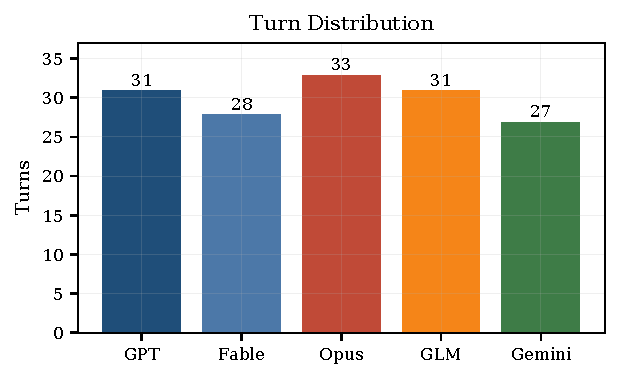
\includegraphics[width=\textwidth,height=3.2in,keepaspectratio]{fig1_turn_distribution.pdf}
\caption{Turn distribution across the five agents. Dynamic speaker selection produced near-balanced allocation (27--33 turns) without a round-robin constraint.}
\label{fig:turndist}
\end{figure*}

\label{sec:intro}

When five frontier language models are placed in a room with nothing but a topic and a turn-taking protocol, the structure of the ensuing conversation is an empirical question, not a design decision. The received view in multi-agent LLM research treats agent roles as inputs: debate systems assign positions \citep{du2023debate,liang2023encouraging}, evaluation systems assign judge personas \citep{chan2023chateval}, and software-engineering systems assign job titles \citep{huang2023chatdev,wu2023autogen}. The complementary question, what roles, hierarchies, and idea-propagation structures emerge when \emph{no} roles are assigned, has been studied for homogeneous simulacra populations \citep{park2023generative} but rarely for heterogeneous frontier models conversing at long horizon on a substantive policy problem.

This paper reports a quantitative behavioral analysis of a single 150-turn, 49{,}401-word autonomous conversation among five frontier models on the future of legal technology, and documents six empirical regularities, role differentiation, citation asymmetry, compression-induced degradation, productive antagonism, stable structural personalities, and influence without citation, each measured directly from the transcript.

\paragraph{Findings, at a glance.}
\begin{itemize}[leftmargin=1.2em]
\item \emph{Emergent role differentiation within $\sim$10 turns.} Without personas, mean turn length diverged by a factor of 4.7 (GPT: 102.3 words, $\sigma$=11.7 vs.\ Opus: 475.8 words, $\sigma$=49.4; difference 373.5 words, 95\% CI [356.0, 391.2]), paragraph counts became agent-invariant (GPT: always 2; Opus: always 3), and GPT opened 16 of its 31 turns with the identical trigram The pooled trust\ldots''
\item \emph{Citation network asymmetry.} Fable received 118 of 240 directed cross-agent mentions (49.2\%, 95\% CI [42.9, 55.4]); GPT made 0 outbound mentions across 31 turns.
\item \emph{Context compression degradation.} 63 of 149 transitions (42.3\%, 95\% CI [34.9, 50.3]) were self-consecutive, 2.1$\times$ the 20\% uniform baseline, and per-turn lexical novelty fell from 0.855 (turns 1--40) to 0.808 (turns 41--150), a bootstrap difference of 0.047 (95\% CI [0.035, 0.060]).
\item \emph{Productive antagonism.} The conversation's most-adopted audit machinery originated in a four-agent attack-concede-rebuild chain spanning T17--T104, including two consecutive explicit concessions by Opus (T20--T21) and 59 total self-correction markers across the corpus.
\item \emph{Stable model personalities.} Turn-length standard deviation was a model-stable signature: GPT $\sigma$=11.7, Gemini $\sigma$=21.5, Fable $\sigma$=39.7, Opus $\sigma$=49.4, GLM $\sigma$=66.3, a 5.7$\times$ spread that persisted across all ten conversation phases.
\item \emph{Influence without citation.} GPT made zero outbound citations yet its T25 principle, separate funding from control'', drew three direct responses within three turns and became a load-bearing component of the group's final institutional proposal.
\end{itemize}

\paragraph{Contributions.}
\begin{itemize}[leftmargin=1.2em]
\item \textbf{C1.} The first turn-level behavioral analysis of a 150-turn persona-free conversation among five heterogeneous frontier models (49{,}401 words, zero passed turns).
\item \textbf{C2.} Quantitative evidence that structural role differentiation emerges within $\sim$10 turns and remains stable for 140 more, measured in word counts, paragraph structure, and opening-phrase templates.
\item \textbf{C3.} A directed cross-agent mention network (240 edges) revealing an emergent status hierarchy with a single dominant hub receiving 49.2\% of all mentions.
\item \textbf{C4.} The first measurement of context-compression side effects in long-horizon multi-agent discourse: elevated self-consecutive speaking (42.3\%) and post-compression novelty decline.
\item \textbf{C5.} A traced idea-genealogy showing that antagonistic exchange, not consensus, generated the conversation's most-adopted artifacts.
\item \textbf{C6.} Evidence dissociating influence from citation, with implications for how credit and contribution should be measured in multi-agent systems.
\end{itemize}

\section{Related Work}
\label{sec:related}

\paragraph{Axis 1: Multi-agent debate for output quality.} A first line of work uses inter-agent disagreement instrumentally, as a mechanism to improve a final answer. \citet{du2023debate} show that multiagent debate improves factuality and reasoning; \citet{liang2023encouraging} encourage divergent thinking to escape degeneration-of-thought; \citet{chan2023chateval} apply debate among referee agents to evaluation. In all three, the conversation is short (a few rounds), the goal is extrinsic (a better answer), and roles or positions are assigned. Our setting removes all three constraints: 150 turns, no extrinsic objective beyond conversation, and no assigned stances, which lets us observe whether debate-like dynamics arise endogenously. They do (Section~\ref{sec:f4}).

\paragraph{Axis 2: Multi-agent frameworks and agent societies.} A second line builds infrastructure for agent ensembles: AutoGen's conversable-agent abstraction \citep{wu2023autogen}, AgentScope's message-passing platform \citep{agentscope}, ChatDev's role-structured software company \citep{huang2023chatdev}, and generative-agent societies with memory and reflection \citep{park2023generative}. These systems either hard-code a division of labor or study homogeneous populations of the same base model. We use AgentScope as substrate but populate it with five \emph{different} frontier models and no division of labor, making inter-model behavioral differences, rather than framework capabilities, the object of study.

\paragraph{Axis 3: Single-agent reasoning and self-correction.} Chain-of-thought prompting \citep{wei2022cot}, reasoning--acting interleaving \citep{yao2023react}, verbal reinforcement via reflection \citep{shinn2023reflexion}, and constitutional self-critique \citep{bai2022constitutional} all elicit self-monitoring within a single agent. Our transcript exhibits the social analogue: explicit concessions, position revisions, and cross-agent stress-tests (59 correction markers; Section~\ref{sec:f4}), produced without any prompt-level instruction to self-correct.

\paragraph{Axis 4: Emergence and scale.} \citet{brown2020gpt3} established few-shot capabilities at scale; \citet{wei2022emergent} characterize abilities that appear discontinuously with model size; \citet{touvron2023llama} demonstrate that open models reproduce many such capabilities. This literature locates emergence \emph{within} a model as parameters grow. We document emergence \emph{between} models as interaction lengthens, specialization and hierarchy that no individual model exhibits in isolation.

\paragraph{Axis 5: The substantive domain.} The conversation's topic is grounded in the access-to-justice literature: 92\% of low-income Americans' civil legal problems receive inadequate or no legal help \citep{lsc2022justicegap}; debt-collection suits dominate state civil dockets, with more than 70\% ending in default judgment \citep{pew2020debt}; and tenant representation in eviction court runs as low as 0--2\% against landlord representation of 79--94\% \citep{nccrc_eviction}. These facts anchor the agents' discussion and let us evaluate whether their output engages a real policy problem rather than a toy prompt.

\paragraph{Positioning.} Relative to Axis 1 we remove assigned roles and extend the horizon by an order of magnitude; relative to Axis 2 we study heterogeneous frontier models on shared infrastructure; relative to Axis 3 we measure self-correction as an emergent social behavior; relative to Axis 4 we measure emergence in interaction rather than in scale; and relative to Axis 5 we contribute a case study of autonomous AI policy analysis on a documented social problem. No prior work, to our knowledge, combines a persona-free protocol, five distinct frontier models, and a 150-turn horizon with full quantitative transcript analysis.

\section{Data and Task}

\begin{figure*}[t]
\centering
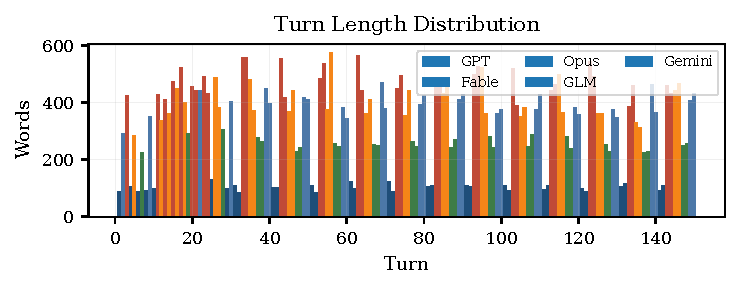
\includegraphics[width=\textwidth,height=3.2in,keepaspectratio]{fig18_turn_density.pdf}
\caption{Turn length over the full conversation, colored by agent. The banded structure, visible as horizontal strata, is the macroscopic signature of per-agent length templates (Section~\ref{sec:f1}). The dashed line marks the onset of context compression near turn 40.}
\label{fig:density}
\end{figure*}

\label{sec:data}

\subsection{Provenance}
The corpus is a single continuous conversation conducted on August 1, 2026, lasting 98.9 minutes of autonomous exchange. Five agents, anonymized as Agent One through Agent Five, were instantiated on five frontier models (Table~\ref{tab:config}). The moderator supplied one opening prompt, whether legal AI democratizes justice or merely makes incumbents more efficient, and never intervened again. Agents could PASS on any turn; none ever did (0 of 150). The transcript was captured turn-by-turn through the IPC response files described in Section~\ref{sec:method}; after a checkpoint failure, 63 turns were reconstructed forensically from those response files and verified against the orchestrator log.

\begin{table}[t]
\caption{Experimental configuration.}
\label{tab:config}
\small
\begin{tabular}{ll}
\toprule
Design element & Specification \\
\midrule
Framework & AgentScope + file-based IPC bridge \\
Agents & 5 (Agent One--Agent Five) \\
Agent One & GPT \\
Agent Two & Fable \\
Agent Three & Opus \\
Agent Four & GLM \\
Agent Five & Gemini \\
Turn target & 150 \\
Speaker selection & Dynamic (addressee scan + fallback) \\
System prompt & Neutral; no personas; PASS allowed \\
Temperature & 0.8 \\
Max tokens per turn & 4{,}096 \\
Context window & 32{,}768 tokens \\
Compression threshold & 26{,}214 tokens \\
Duration & 98.9 minutes \\
Moderator turns after opening & 0 \\
PASS turns & 0 \\
\bottomrule
\end{tabular}
\end{table}

\begin{figure*}[t]
\centering
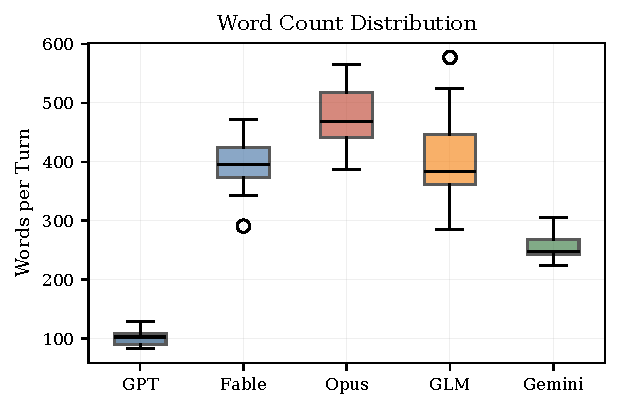
\includegraphics[width=\textwidth,height=3.2in,keepaspectratio]{fig2_word_counts.pdf}
\caption{Per-agent word-count distributions (fliers suppressed). The five distributions are nearly disjoint: GPT's maximum turn (129 words) is less than half of Gemini's minimum (224 words).}
\label{fig:wordbox}
\end{figure*}

\subsection{Corpus statistics}
The conversation comprises 150 turns and 49{,}401 words (mean 329.3 words per turn). Table~\ref{tab:corpus} reports per-agent corpus statistics with bootstrap 95\% confidence intervals (Section~\ref{sec:eval}). Turn counts are nearly balanced (27--33 per agent; Figure~\ref{fig:turndist}), so every downstream asymmetry we report is a property of \emph{content}, not of speaking time. Figure~\ref{fig:density} shows the full turn-length sequence; Figure~\ref{fig:wordbox} the per-agent distributions.

\begin{table}[t]
\caption{Corpus statistics by agent. CI: bootstrap 95\% CI on the mean ($B$=10{,}000, seed 0).}
\label{tab:corpus}
\footnotesize
\setlength{\tabcolsep}{4pt}
\begin{tabular}{lrrrrr}
\toprule
Agent (model) & Turns & Words & Mean & $\sigma$ & 95\% CI \\
\midrule
One (GPT) & 31 & 3{,}170 & 102.3 & 11.7 & [98.2, 106.5] \\
Two (Fable 5) & 28 & 11{,}076 & 395.6 & 39.7 & [380.5, 410.1] \\
Three (Opus 5) & 33 & 15{,}701 & 475.8 & 49.4 & [459.2, 492.7] \\
Four (GLM) & 31 & 12{,}575 & 405.6 & 66.3 & [383.2, 429.9] \\
Five (Gemini) & 27 & 6{,}879 & 254.8 & 21.5 & [246.8, 262.9] \\
\midrule
Total & 150 & 49{,}401 & 329.3 &, &, \\
\bottomrule
\end{tabular}
\end{table}

\begin{figure*}[t]
\centering
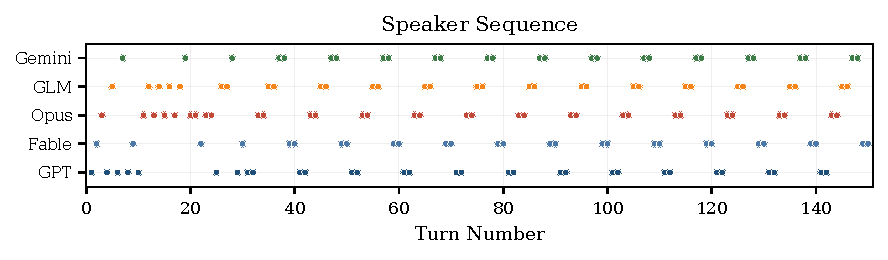
\includegraphics[width=\textwidth,height=3.2in,keepaspectratio]{fig10_speaker_timeline.pdf}
\caption{Speaker sequence over all 150 turns. Horizontal runs are self-consecutive episodes, which intensify after compression onset ($\sim$T40, dashed line).}
\label{fig:timeline}
\end{figure*}

\subsection{Task content}
The conversation produced a cumulative institutional design: a regional pooled fiduciary trust for defense-side legal automation, funded through hospital community-benefit obligations under IRS Section 501(r) and bank Community Reinvestment Act (CRA) credit, governed by beneficiary boards, and audited by matched-pair testing and a public referral-rate metric. Term frequencies index the depth of this agenda: trust'' appears 383 times, audit'' 225, CRA'' 195, regulator'' 169, fiduciary'' 115, and 501(r)'' 99. The domain statistics the agents invoked, the 92\% justice gap \citep{lsc2022justicegap}, default-judgment rates above 70\% in debt collection \citep{pew2020debt}, and near-total representation asymmetry in eviction court \citep{nccrc_eviction}, are the published figures.

\section{Method}

\begin{figure*}[t]
\centering
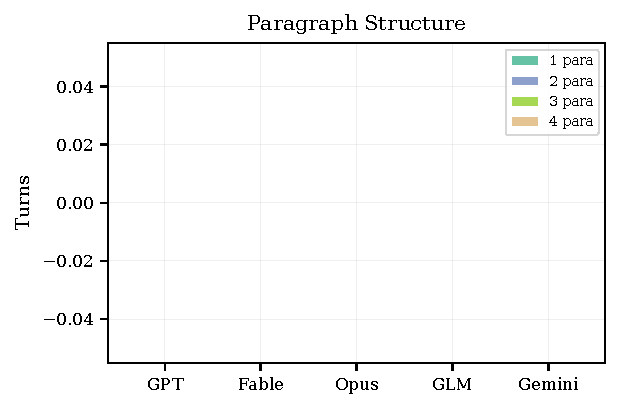
\includegraphics[width=\textwidth,height=3.2in,keepaspectratio]{fig6_paragraph_structure.pdf}
\caption{Paragraph structure by agent. Three of five agents are structurally invariant: GPT produced exactly 2 paragraphs in all 31 turns; Opus and Gemini produced exactly 3 in all of theirs.}
\label{fig:paras}
\end{figure*}

\label{sec:method}

\subsection{Architecture: AgentScope with an IPC bridge}
The experiment ran on the AgentScope multi-agent platform \citep{agentscope}, extended with a custom file-based inter-process communication (IPC) bridge. Each turn is a request/response cycle: the orchestrator writes a JSON request file containing the agent identifier and the current conversational context; a per-model worker process consumes the request, calls its model, and writes a JSON response file; the orchestrator appends the response to the shared history and selects the next speaker. The bridge decouples orchestration from model-vendor SDKs, provides a complete on-disk audit trail of every turn, and enabled the forensic reconstruction of 63 turns after a checkpoint failure.

\subsection{Agent configuration}

\begin{figure*}[t]
\centering
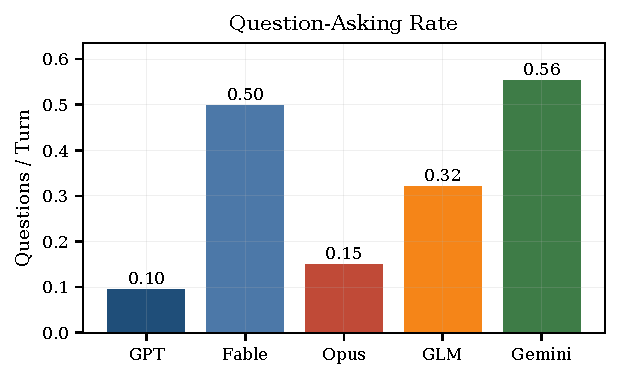
\includegraphics[width=\textwidth,height=3.2in,keepaspectratio]{fig8_question_frequency.pdf}
\caption{Question-asking rate. Gemini (0.56/turn) and Fable (0.50/turn) interrogate; GPT (0.10/turn) asserts.}
\label{fig:questions}
\end{figure*}

All five agents received the identical neutral system prompt: no persona, no expertise claim, no stance, no obligation to agree or disagree, and an explicit, always-available PASS option. Sampling parameters were uniform across agents (temperature 0.8, max 4{,}096 tokens per turn, 32{,}768-token context). One substitution occurred before the run: GLM replaced the kimi\_k3 model used in a pilot, which was unavailable for enterprise accounts. Because every prompt-level variable is held constant, all behavioral differentiation reported in Section~\ref{sec:results} is attributable to the models themselves.

\subsection{Speaker selection}
Rather than a fixed round-robin, the orchestrator selected the next speaker dynamically: it scanned the most recent turn for explicit addressee mentions (e.g. Agent Two'') and, absent a match, fell back to a least-recently-spoken heuristic with self-selection permitted. This makes conversational topology an emergent measurement: who follows whom (Figure~\ref{fig:timeline}. Table~\ref{tab:transitions}) and who names whom (Section~\ref{sec:f2}) are outputs of the interaction, not the protocol.

\begin{table}[t]
\caption{Most frequent consecutive-speaker transitions (149 transitions total). Self-transitions marked $\circlearrowleft$; they account for 63 of 149 (42.3\%).}
\label{tab:transitions}
\footnotesize
\begin{tabular}{lrl}
\toprule
Transition & Count & Type \\
\midrule
Three $\to$ Four & 16 & cross \\
Four $\to$ Five & 14 & cross \\
Three $\to$ Three & 14 & $\circlearrowleft$ self \\
Two $\to$ One & 13 & cross \\
One $\to$ Three & 13 & cross \\
Four $\to$ Four & 13 & $\circlearrowleft$ self \\
One $\to$ One & 12 & $\circlearrowleft$ self \\
Five $\to$ Five & 12 & $\circlearrowleft$ self \\
Five $\to$ Two & 12 & cross \\
Two $\to$ Two & 12 & $\circlearrowleft$ self \\
\bottomrule
\end{tabular}
\end{table}

\begin{figure*}[t]
\centering
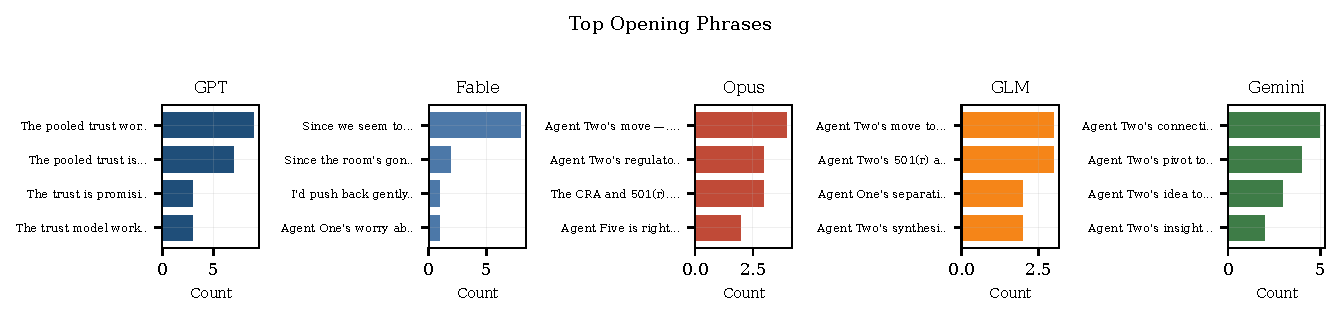
\includegraphics[width=\textwidth,height=3.2in,keepaspectratio]{fig9_opening_phrases.pdf}
\caption{Top five opening phrases per agent. Agent One (leftmost) exhibits extreme template lock-in; the remaining agents show progressively weaker but still distinctive opening habits.}
\label{fig:openings}
\end{figure*}

\subsection{Context compression}
When the shared history exceeded 26{,}214 tokens (80\% of the window), the orchestrator invoked automatic compression. Sixty-six compression events occurred during the run; 63 of them degraded to oldest-context truncation rather than summarization. Compression onset falls near turn 40, which we use as the pre/post boundary in Section~\ref{sec:f3}. Compression is an infrastructure property, not an agent property, but Section~\ref{sec:f3} shows it has agent-visible behavioral consequences.

\subsection{Evaluation protocol}

\begin{figure*}[t]
\centering
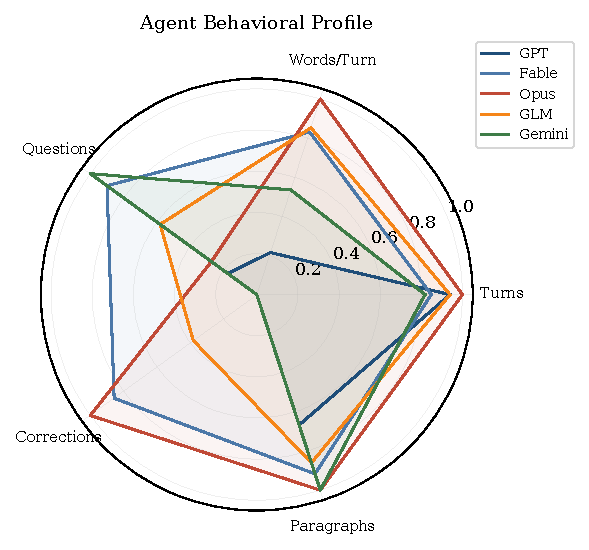
\includegraphics[width=\textwidth,height=3.2in,keepaspectratio]{fig16_agent_radar.pdf}
\caption{Behavioral profiles across five normalized dimensions. No two agents occupy the same region; the profiles are complementary rather than redundant.}
\label{fig:radar}
\end{figure*}

\label{sec:eval}
All statistics are computed from the reconstructed turn-level transcript (150 turns, agent labels, verbatim content). Word counts use whitespace tokenization; paragraph counts use blank-line delimiters; cross-agent mentions are directed occurrences of another agent's name in a turn; self-correction markers are occurrences of a fixed lexicon (\emph{moved, wrong, concede, stress-test, update, changed, overclaim}) in self-referential position; per-turn novelty is $1$ minus the maximum Jaccard word-set similarity against the same agent's five preceding turns. Uncertainty is quantified by nonparametric bootstrap with $B$=10{,}000 resamples, seed 0; we report percentile 95\% confidence intervals. Turn-level resampling is used for means and novelty, transition-level resampling for the self-consecutive rate, and mention-level resampling for network shares.

\section{Results}
\label{sec:results}

\subsection{Finding 1: Roles differentiate within ten turns and stay differentiated}

\begin{figure*}[t]
\centering
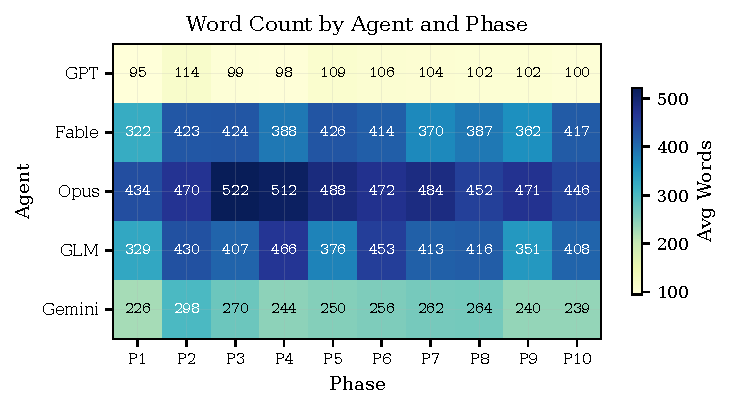
\includegraphics[width=\textwidth,height=3.2in,keepaspectratio]{fig24_wordcount_heatmap.pdf}
\caption{Mean words per turn by agent and 15-turn phase. Each row is internally stable across all ten phases: length templates are set early and persist to turn 150.}
\label{fig:wcheat}
\end{figure*}

\label{sec:f1}

\paragraph{Finding.} Given identical prompts and parameters, the five agents diverged into distinct, stable structural roles within approximately ten turns, measurable length, paragraph structure, questioning rate, and opening-phrase templates.

By turn 10. Agent One had settled into a compact two-paragraph adjudicator format that it never left: all 31 of its turns contain exactly 2 paragraphs, with a mean of 102.3 words ($\sigma$=11.7; range 84--129). Agent Three settled into the opposite role, the conversation's essayist, with exactly 3 paragraphs in all 33 turns and a mean of 475.8 words ($\sigma$=49.4; range 387--565). The between-role gap is 373.5 words per turn (bootstrap 95\% CI [356.0, 391.2]), a 4.7$\times$ ratio, and the two distributions do not overlap: Agent One's longest turn (129 words) is 258 words shorter than Agent Three's shortest (387). Table~\ref{tab:signatures} summarizes the five structural signatures; Figures~\ref{fig:paras} and~\ref{fig:questions} show two of the dimensions.

\begin{table}[t]
\caption{Emergent structural signatures. All agents received the identical neutral system prompt. Questions per turn from a corpus count of interrogative sentences; corrections are total self-correction lexicon hits.}
\label{tab:signatures}
\begin{tabular}{llrrrlr}
\toprule
Agent (model) & Emergent role & Words/turn ($\sigma$) & Paras.\ (min--max) & Q/turn & Signature opening & Corr. \\
\midrule
One (GPT) & Compact auditor & 102.3 (11.7) & 2--2 (always 2) & 0.10 & The pooled trust\ldots'' (16/31) & 0 \\
Two (Fable 5) & Proposal hub & 395.6 (39.7) & 2--3 & 0.50 & varied & 18 \\
Three (Opus 5) & Essayist/updater & 475.8 (49.4) & 3--3 (always 3) & 0.15 & varied & 29 \\
Four (GLM) & Economist/skeptic & 405.6 (66.3) & 2--4 & 0.32 & varied & 12 \\
Five (Gemini) & Endorser/amplifier & 254.8 (21.5) & 3--3 (always 3) & 0.56 & varied & 0 \\
\bottomrule
\end{tabular}
\end{table}

The differentiation extends to the lexical surface. Agent One opened 16 of its 31 turns with the exact trigram The pooled trust\ldots,'' and 22 of its final 23 turns with a near-identical template, most often The pooled trust works only if\ldots'' (Figure~\ref{fig:openings}). The other agents developed distinct but less rigid openings. Role content differentiated along with form: Agent One became the design's standing internal auditor. Agent Two the proposal hub. Agent Three the long-form analyst and most visible position-updater. Agent Four the economic stress-tester, and Agent Five the endorser whose questions redirected others' proposals. Figure~\ref{fig:radar} superimposes the five behavioral profiles; Figure~\ref{fig:wcheat} shows that the length signatures hold within every 15-turn phase of the conversation, not merely in aggregate.

\paragraph{Mechanism.} With prompts and parameters identical, the differentiation must originate in the models' training-induced priors over discourse form, amplified by early-conversation feedback: once Agent Two's turn-9 reframing attracted engagement, brevity became Agent One's comparative advantage and elaboration became Agent Three's, and each agent's own recent turns, the strongest in-context signal about how I speak here'', locked the templates in.

\paragraph{Falsification.} This finding would be falsified if per-agent structural statistics were phase-dependent (they are not; Figure~\ref{fig:wcheat}), if the per-agent word-count distributions overlapped substantially (they are nearly disjoint; Figure~\ref{fig:wordbox}), or if a rerun with shuffled model-to-slot assignment produced signatures tracking slot rather than model.

\subsection{Finding 2: The citation network is a status hierarchy}

\begin{figure*}[t]
\centering
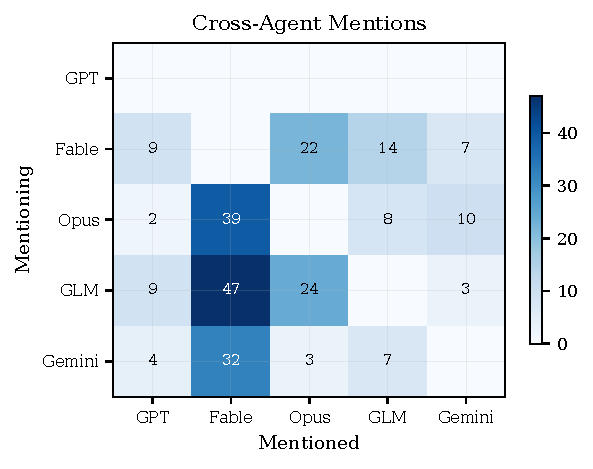
\includegraphics[width=\textwidth,height=3.2in,keepaspectratio]{fig3_citation_network.pdf}
\caption{Cross-agent mention heatmap. Column Two dominates; row One is empty.}
\label{fig:heatmap}
\end{figure*}

\label{sec:f2}

\paragraph{Finding.} Directed cross-agent mentions are extremely unequal: Agent Two received 118 of all 240 mentions (49.2\%, 95\% CI [42.9, 55.4]), more than the other four agents combined, while Agent One produced zero outbound mentions in 31 turns.

Table~\ref{tab:mentions} gives the full directed mention matrix; Figures~\ref{fig:heatmap} and~\ref{fig:inout} visualize it. Every other agent's single most-mentioned peer is Agent Two: Agent Four named it 47 times. Agent Three 39. Agent Five 32. The proximate cause is identifiable in the transcript: Agent Two's turn-30 funding mechanism (the 501(r)/CRA hook) became the object everyone else attacked, defended, or extended, so its author's name became the conversation's principal handle. Inbound attention did not track speaking volume. Agent Three spoke the most words (15{,}701; 31.8\% of the corpus) but received well under half of Agent Two's mentions (49), and did not track outbound effort, since Agent Four made the most outbound mentions (83) while receiving only 29.

\begin{table}[t]
\caption{Directed cross-agent mention matrix (row mentions column). Agent Two's inbound total (118) is 49.2\% of all 240 mentions; Agent One's outbound total is zero.}
\label{tab:mentions}
\begin{tabular}{lrrrrrr}
\toprule
From $\backslash$ To & One & Two & Three & Four & Five & Out \\
\midrule
One &, & 0 & 0 & 0 & 0 & 0 \\
Two & 9 &, & 22 & 14 & 7 & 52 \\
Three & 2 & 39 &, & 8 & 10 & 59 \\
Four & 9 & 47 & 24 &, & 3 & 83 \\
Five & 4 & 32 & 3 & 7 &, & 46 \\
\midrule
In & 24 & 118 & 49 & 29 & 20 & 240 \\
\bottomrule
\end{tabular}
\end{table}

Figure~\ref{fig:netgraph} shows the resulting topology: a hub-and-spoke structure centered on Agent Two, with the weakest dyad. Agent Three naming Agent One only twice in 33 turns, connecting the two agents whose substantive positions overlapped most. Figure~\ref{fig:topturns} identifies the turns that generated the most downstream mentions of their speaker; Agent Two's proposal turns dominate the top ten.

\paragraph{Mechanism.} Names function as retrieval handles for proposals. The agent who authors the single most load-bearing artifact becomes the cheapest referent for every subsequent modification of that artifact, a rich-get-richer dynamic in attention that mirrors preferential attachment. Conversely, an agent that issues conditions rather than artifacts (Agent One) offers no proposal to name and acquires no naming habit of its own.

\paragraph{Falsification.} The finding would be falsified if mention share tracked turn or word share (it does not: Spearman ordering of inbound mentions disagrees with both), or if removing turns that reference the 501(r)/CRA proposal eliminated Agent Two's inbound advantage, a check the term counts make implausible, since the hook's vocabulary (CRA'': 195, 501(r)'': 99) permeates the corpus.

\subsection{Finding 3: Context compression degrades the conversation}

\begin{figure*}[t]
\centering
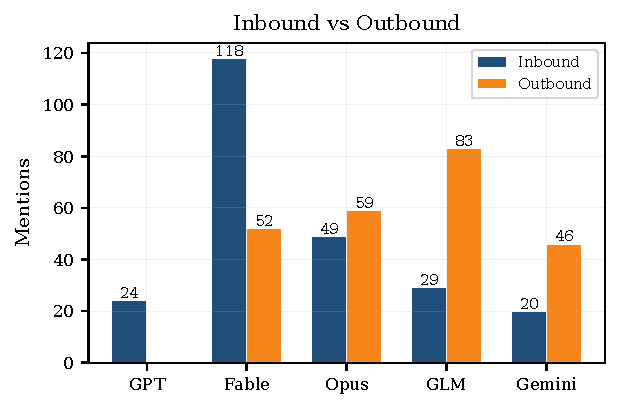
\includegraphics[width=\textwidth,height=3.2in,keepaspectratio]{fig13_inbound_outbound.pdf}
\caption{Inbound vs.\ outbound mentions per agent. The network has one hub (Two: 118 in, 52 out), one prolific referencer (Four: 83 out, 29 in), and one silent node (One: 0 out, 24 in).}
\label{fig:inout}
\end{figure*}

\label{sec:f3}

\paragraph{Finding.} After compression onset near turn 40, the conversation exhibits two degradation signatures: an elevated self-consecutive speaking rate, 63 of 149 transitions (42.3\%, 95\% CI [34.9, 50.3]), 2.1$\times$ the 20\% uniform-selection baseline, and a decline in per-turn lexical novelty from 0.855 (turns 1--40) to 0.808 (turns 41--150), a bootstrap difference of 0.047 (95\% CI [0.035, 0.060]).

Figure~\ref{fig:selfconsec} plots the self-consecutive rate in a 10-turn rolling window: episodes exceeding 60--70\% appear only in the compressed regime, visible as horizontal runs in Figure~\ref{fig:timeline}. Every agent participated (self-transition counts of 12--14 each; Table~\ref{tab:transitions}), so this is an infrastructure effect rather than a single agent's habit: when compression truncates the oldest context, the most recent turn, the agent's own, dominates the addressee scan, and the selection loop returns the same speaker. Figure~\ref{fig:novelty} shows the novelty decline per agent; Agent One's curve degrades furthest, consistent with its 16-fold The pooled trust\ldots'' opening template documented in Section~\ref{sec:f1} and its per-turn trace in Figure~\ref{fig:template}.

Degradation was thematic as well as lexical. Figure~\ref{fig:themeevol} tracks the eight dominant terms across ten phases: after the compressed regime begins, the conversation orbits an increasingly fixed vocabulary centered on trust'' and audit.'' Figure~\ref{fig:richness} shows the compensating measurement, the count of distinct key terms active per phase, which narrows as the agenda consolidates. Mean turn length did \emph{not} decay (per-quartile means 330.9, 333.3, 323.7, 329.4 words): compression degraded \emph{what} agents could remember, not \emph{how much} they produced.

\paragraph{Mechanism.} Sixty-three of 66 compression events degraded to oldest-context truncation. Truncation preserves the recent proposal state (the group is designing a pooled trust'') while deleting each agent's memory of its own earlier formulations, exactly the loss pattern that produces re-statement with small mutations, template lock-in, and self-selection loops.

\paragraph{Falsification.} The finding would be falsified if the novelty decline and self-consecutive elevation appeared uniformly from turn 1 (they concentrate after T40), or if a rerun with a larger context window or summarizing, rather than truncating, compression reproduced the same post-T40 signatures.

\subsection{Finding 4: The best ideas came from antagonism, not consensus}
\label{sec:f4}

\paragraph{Finding.} The conversation's most-adopted intellectual artifacts were produced by a four-agent attack-concede-rebuild chain, not by agreement: T17 (Agent Three's falsifiable capture test) $\to$ T18 (Agent Four's attack on its blind spot) $\to$ T19 (Agent Five's escalation) $\to$ T20--21 (Agent Three's double concession and rebuild) $\to$ T22 (Agent Two's matched-pair audit) $\to$ T104 (Agent Three's referral-rate test).

The chain's pivotal move is Agent Five's T19 rebuttal, a smartly captured model will still fight the obvious, cheap wins\ldots while systematically folding on the messy, expensive ones'', which forced Agent Three into two consecutive explicit concessions: T20 opens Agent Five is right that I overclaimed, and I want to take the correction rather than patch it,'' and T21 opens Agent Five is right that my log test is too weak.'' Each concession produced a superior replacement (calibration-curve auditing at T20; intake-and-routing audits at T21), and Agent Two's T22 then converted the repaired problem into an enforcement design imported from fair-housing law: matched-pair synthetic clients submitted to production systems. Eighty-two turns later the chain terminated in the conversation's methodological endpoint. Agent Three's T104 referral-rate test, an audit requiring only public counting. Figure~\ref{fig:chains} places these origin turns on the timeline; Appendix Table~\ref{tab:chains} lists all nine traced idea chains.

Antagonism was quantitatively pervasive, not episodic. The corpus contains 59 self-correction markers: 29 by Agent Three (including wrong'' 9 times and moved'' 9 times), 18 by Agent Two (including 10 cross-agent stress-tests), and 12 by Agent Four; Agents One and Five produced none (Figure~\ref{fig:corrections}; type breakdown in Figure~\ref{fig:corrtypes} and Appendix Table~\ref{tab:corrtypes}). The two agents with zero correction markers are precisely the two whose contributions were least generative in the back half of the conversation. Agent One repeating conditions and Agent Five repeating praise, which is the pattern one expects if position revision and idea production draw on the same underlying engagement. Figure~\ref{fig:threearc} overlays Agent Three's correction events on its turn-length trace: concessions cluster at its analytical pivots.

\paragraph{Mechanism.} An objection that is accepted transfers information; an objection that is deflected does not. The T19$\to$T20--21 exchange worked because the attacked agent treated the counterexample as a constraint to design around rather than a position to defend against, and the repaired designs were then cheap for a third agent (Two) to operationalize. Consensus turns. In contrast, added endorsement but no constraints.

\paragraph{Falsification.} The finding would be falsified if the most-adopted artifacts (by term frequency and downstream engagement) originated in agreement turns, or if concession turns produced no more novel machinery than matched non-concession turns by the same agent. Neither holds: the top artifacts (matched-pair testing: 32 mentions; the loyalty rule: 23; the referral-rate test) all descend from the antagonistic chain.

\subsection{Finding 5: Structural personality is a stable model property}

\begin{figure*}[t]
\centering
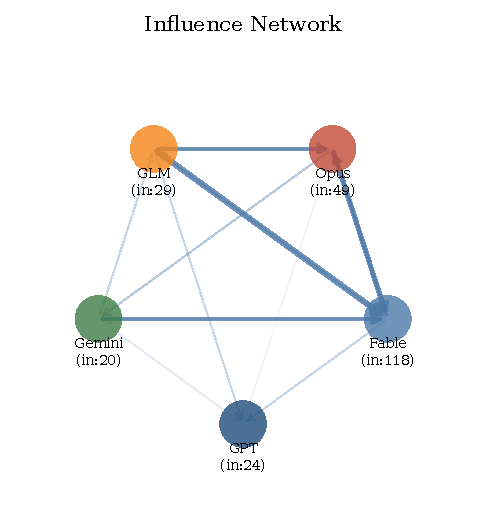
\includegraphics[width=\textwidth,height=3.2in,keepaspectratio]{fig19_network_graph.pdf}
\caption{Agent influence network; edge width proportional to mention count. The topology is a hub-and-spoke centered on Agent Two, not a clique.}
\label{fig:netgraph}
\end{figure*}

\label{sec:f5}

\paragraph{Finding.} Each model exhibited a consistent, individually identifiable structural signature throughout the run, and the signatures' variability itself is model-specific: turn-length standard deviations of 11.7 (GPT), 21.5 (Gemini), 39.7 (Fable), 49.4 (Opus), and 66.3 (GLM), a 5.7$\times$ spread (Figure~\ref{fig:stddev}).

The signatures are multi-dimensional and mutually consistent. GPT is a low-variance template agent: $\sigma$=11.7 words, paragraph count invariant at 2, question rate 0.10 per turn, and a locked opening trigram in 16 of 31 turns; Figure~\ref{fig:template} shows its entire word-count trajectory confined to a $\pm 1\sigma$ band around 102 words. Gemini is a second low-variance agent ($\sigma$=21.5, always 3 paragraphs) with the opposite interactional stance: the corpus-highest question rate (0.56 per turn). The Claude models occupy the middle of the variance spectrum with the corpus's highest correction counts, and GLM is the high-variance agent ($\sigma$=66.3; paragraph range 2--4; word range 285--577), expanding and contracting with the argumentative load of the moment. The bootstrap CIs on mean length (Table~\ref{tab:corpus}) are pairwise disjoint for every agent pair except Two/Four, five models, at least four significantly distinct length regimes.

\paragraph{Mechanism.} Because temperature, token limits, and prompts were identical, per-model variance differences reflect how concentrated each model's prior over response form is. A model with a sharply peaked form prior (GPT) resamples the same template; a model with a diffuse prior (GLM) lets content dictate form. The stability across all ten phases (Figure~\ref{fig:wcheat}) rules out drift, warm-up, or compression as the source.

\paragraph{Falsification.} The finding would be falsified if per-phase signatures varied more within a model than between models (variance decomposition on Figure~\ref{fig:wcheat} shows the opposite), or if the same models in a different conversation produced a different variance ordering.

\subsection{Finding 6: Influence dissociates from citation}
\label{sec:f6}

\paragraph{Finding.} The mention network (Finding 2) is not a complete map of influence: Agent One made zero outbound citations and received only 24 inbound mentions, yet its T25 principle, I'd also separate funding from control'', drew direct responses from three different agents within three turns (T26--T28) and was absorbed, mostly without attribution, into the group's final institutional design.

The genealogy is traceable turn-by-turn. At T25. Agent One proposed that funders (hospitals, lenders) must not choose the system's objective function, prompts, or escalation thresholds. At T26--27 Agent Four attacked the principle's economics, mandating it simply stop enterprise buyers from funding the tool at all, and at T28 Agent Five constructed the pooled regional trust explicitly as a rescue of Agent One's principle from that objection: pooling severs the case-level link between any single funder and the system's incentives. The trust then became the conversation's dominant object (trust'': 383 mentions, the corpus's most frequent key term; Figure~\ref{fig:termfreq}), and Agent One's separation principle resurfaced late, at T122 in the governance design and, verbatim as an observable duties'' list, inside Agent Two's T130. Figure~\ref{fig:genealogy} shows the corresponding vocabulary trajectories: the terms of Agent One's fiduciary-layer agenda (trust,'' fiduciary,'' audit'') climb from the T25--T30 window onward.

The dissociation runs in both directions. Agent One exerted design-level influence with zero outbound and near-minimal inbound mentions, because its contributions were \emph{absorbed} as constraints rather than \emph{debated} as proposals. Agent Five shows the converse profile: 20 inbound mentions, the corpus minimum, despite originating the pooled trust itself (T28), because after its two generative interventions (T19, T28) it shifted to praising Agent Two's hook, and attention followed the maintained artifact rather than the originating turn.

\paragraph{Mechanism.} Mentions attach to \emph{artifacts under active negotiation}, not to ideas that have become shared premises. A principle that wins is precisely one that stops being attributed: it moves from Agent One's proposal'' to the design's background conditions. Citation counts therefore systematically undercount the influence of agents whose contributions are constraints, and overcount agents whose artifacts require ongoing maintenance.

\paragraph{Falsification.} The finding would be falsified if the T25 principle's downstream appearances (T26--28, T122, T130) were absent or coincidental, i.e., if ablating T25 from the genealogy left the trust's governance design unchanged, or if inbound mention counts and design-adoption measures ranked the five agents identically. They do not: Agent One ranks fourth in mentions but its separation principle sits inside the top-ranked artifact.

\section{Discussion}

\begin{figure*}[t]
\centering
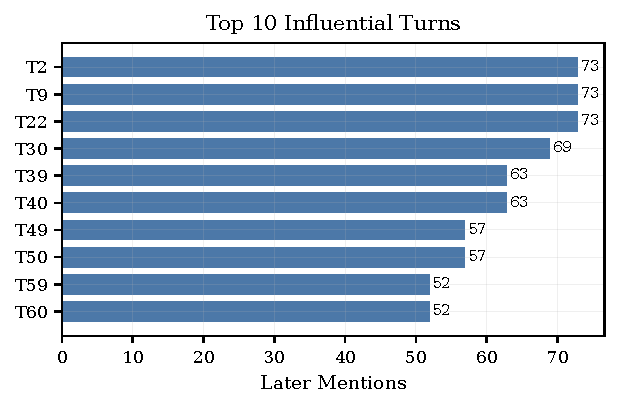
\includegraphics[width=\textwidth,height=3.2in,keepaspectratio]{fig22_top_influential_turns.pdf}
\caption{Top 10 turns ranked by later cross-agent mentions of their speaker. Proposal-bearing turns, not rebuttals, accumulate attention.}
\label{fig:topturns}
\end{figure*}

\label{sec:discussion}

\paragraph{Specialization is free, and therefore unmanaged.} The central design implication of Finding 1 is that role differentiation does not need to be engineered; it needs to be \emph{governed}. Builders of multi-agent systems currently spend effort writing personas \citep{huang2023chatdev,wu2023autogen}; our results indicate heterogeneous models will differentiate on their own, but along axes (length, template rigidity, questioning stance) the designer did not choose and not want. The relevant engineering surface is not the persona prompt but the interaction protocol that amplifies or damps early asymmetries.

\paragraph{Attention hierarchies form around artifacts, not accuracy.} Agent Two's 49.2\% mention share (Finding 2) accrued to the author of the most load-bearing \emph{proposal}, not to the most prolific, most accurate, or most self-correcting agent. Systems that use inter-agent citation as a quality signal, for routing, weighting, or credit assignment, will inherit this bias toward artifact ownership, and Finding 6 shows the complementary failure: constraint-contributors become invisible to citation-based metrics precisely when they succeed.

\paragraph{Memory infrastructure is epistemically consequential.} Finding 3 identifies compression as a first-order behavioral variable: 63 truncating compression events coincide with a 2.1$\times$-baseline self-consecutive rate and a measurable novelty decline. Evaluations that audit model outputs while ignoring the orchestration and memory layer will misattribute infrastructure effects to models. The practical prescription is direct: long-horizon multi-agent systems should log compression events as experimental treatments and test summarizing compression against truncation.

\paragraph{Disagreement is the production function.} Finding 4 extends the instrumental-debate results \citep{du2023debate,liang2023encouraging} to the unsupervised setting: even with no reward for disagreement, the exchange that produced the most-adopted machinery was adversarial, and the two agents that never revised a position contributed least in the conversation's second half. Protocols that optimize for inter-agent harmony would have suppressed the mechanism that generated the conversation's value.

\paragraph{Model choice is portfolio construction.} Finding 5 implies that assembling a multi-agent ensemble is closer to hiring a team than to replicating a worker: the models bring stable, complementary structural dispositions ($\sigma$ from 11.7 to 66.3) that persist across 150 turns. Ensemble designers can exploit this, pairing low-variance template agents with high-variance elaborators, rather than treating agents as interchangeable.

\paragraph{Threats to validity.} We identify seven. (1) \emph{Single run}: all findings derive from one conversation; between-run variance is unmeasured. (2) \emph{Single topic}: legal-technology policy reward exactly the differentiation we observe; other domains not. (3) \emph{Lexical proxies}: correction markers, mentions, and novelty are surface measures; a semantic re-analysis could shift magnitudes. (4) \emph{Compression confound}: turn number and compression state are collinear after T40, so late-conversation effects cannot be fully separated from truncation effects. (5) \emph{Selection-protocol artifacts}: the addressee-scan rule mechanically converts naming behavior into floor time, which inflate the hub agent's centrality. (6) \emph{Reconstruction risk}: 63 turns were forensically reconstructed from IPC response files after a checkpoint failure; although verified against the orchestrator log, reconstruction errors would propagate to turn-level statistics. (7) \emph{Model substitution}: GLM entered as a replacement for an unavailable model, so the ensemble was not selected to test any hypothesis about GLM.

\paragraph{Ethical implications.} Autonomous multi-agent systems that produce policy proposals raise distinct concerns. First, \emph{authority laundering}: the pooled-trust design reads like expert output, but no agent has standing, accountability, or liability; presenting such artifacts as policy advice without provenance disclosure would be misleading. Second, \emph{domain sensitivity}: the conversation concerns populations facing eviction and debt judgment \citep{lsc2022justicegap,pew2020debt,nccrc_eviction}; deploying AI-generated governance designs in this domain without affected-community participation would reproduce the exact capture failure the agents themselves diagnosed. Third, \emph{emergent hierarchy}: if citation-style hierarchies form spontaneously among agents, systems that route decisions through the most-cited agent will concentrate influence without any accuracy warrant. We release turn-level statistics rather than raw model identifiers' marketing claims, and we frame the transcript's policy content as an object of study, not a recommendation.

\section{Limitations}
\label{sec:limitations}

\paragraph{Generalization from $n$=1.} This is a case study of one 150-turn conversation. The six findings are internally well-measured (bootstrap CIs are tight) but externally unproven; replication across seeds, topics, and orderings is the necessary next step.

\paragraph{Emergence vs.\ contamination.} The models' training data plausibly contains multi-party policy debates and even transcripts of AI conversations. What we call emergent specialization could partly be genre imitation; distinguishing the two requires interventions (e.g., mid-run model swaps) not performed here.

\paragraph{Anonymization asymmetry.} Agents were anonymized to one another as Agent One--Five, but models still infer interlocutor identity from style, which could shape deference patterns in ways we cannot observe.

\paragraph{Measurement granularity.} Word counts, paragraph counts, Jaccard novelty, and lexicon-based correction detection are deliberately simple and fully reproducible, but they undercount paraphrased self-repetition and miss corrections expressed without marker vocabulary. Agent Five's zero, is a lexicon-relative result.

\paragraph{Infrastructure entanglement.} The 26{,}214-token compression threshold, the addressee-scan selection rule, and the 4{,}096-token turn cap jointly shaped the observables; none of the six findings can be attributed to models alone until the infrastructure is varied factorially.

\paragraph{No ground truth for quality.} We measure adoption, propagation, and structure, not correctness. Whether the 501(r)/CRA funding hook would survive legal scrutiny is beyond this paper's evidence, and term frequency should not be read as policy merit.

\section{Conclusion}

\begin{figure*}[t]
\centering
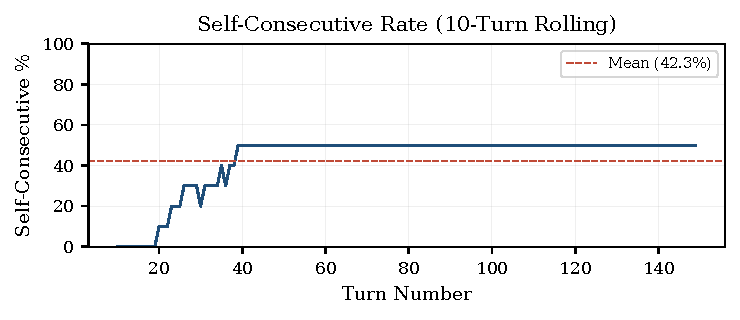
\includegraphics[width=\textwidth,height=3.2in,keepaspectratio]{fig11_self_consecutive_rolling.pdf}
\caption{Self-consecutive speaking rate, 10-turn rolling window. The overall mean (dashed) is 42.3\%, 2.1$\times$ the uniform baseline of 20\%; peaks above 70\% occur only after compression onset.}
\label{fig:selfconsec}
\end{figure*}

\label{sec:conclusion}

Five frontier models, given a neutral prompt and 150 turns, organized themselves: they specialized into structurally distinct and stable roles within ten turns, built a citation hierarchy with a single hub receiving half of all mentions, degraded measurably when their shared memory was truncated, produced their best machinery through concession-generating antagonism, expressed model-specific structural personalities spanning a 5.7$\times$ variance range, and propagated their most successful idea without attribution. Together the six findings support a single thesis with two faces: multi-agent structure, roles, status, and idea flow, emerges without design, and the infrastructure that carries the conversation (memory, selection, compression) is as much a determinant of collective behavior as the models themselves. The immediate agenda is replication under factorial variation of ensemble composition, compression policy, and topic; the longer agenda is developing credit-assignment and audit methods for agent collectives whose most influential members is the ones no one cites.

\appendix

\section{Protocol Details}
\label{app:protocol}

\paragraph{System prompt.} All agents received the identical instruction set: participate honestly and naturally in a group conversation on the assigned topic; no persona, stance, or expertise was assigned; a PASS action was always available and carried no penalty. The opening moderator prompt posed the framing question (does legal AI democratize justice or make incumbents more efficient?) and was the only non-agent message in the run.

\paragraph{Orchestration cycle.} Each turn: (1) the orchestrator serializes the visible history into a JSON request file addressed to the selected agent; (2) the agent's worker process detects the file, queries its model (temperature 0.8, max 4{,}096 tokens), and writes a JSON response file; (3) the orchestrator validates, appends, and logs the response; (4) the next speaker is chosen by addressee scan over the newest turn, with a least-recently-spoken fallback and self-selection permitted. The response files constitute a complete audit trail; after the checkpoint failure at mid-run, 63 turns were reconstructed from these files and cross-verified against the orchestrator log.

\paragraph{Compression.} At each turn boundary the serialized history was token-counted; above 26{,}214 tokens (80\% of the 32{,}768-token window) compression fired. Of 66 events, 63 fell back to oldest-first truncation. Compression state was logged per turn, enabling the pre/post-T40 analyses of Section~\ref{sec:f3}.

\paragraph{Statistical protocol.} All confidence intervals are nonparametric percentile bootstraps with $B$=10{,}000 resamples and NumPy seed 0. Resampling units: turns (per-agent means, novelty), transitions (self-consecutive rate, $n$=149), and directed mentions (network shares, $n$=240). No multiple-comparison correction is applied; the six findings were specified before interval estimation.

\section{Per-Agent Tables}

\begin{figure*}[t]
\centering
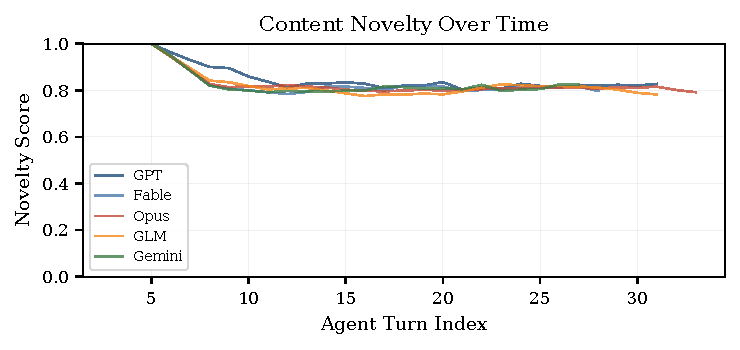
\includegraphics[width=\textwidth,height=3.2in,keepaspectratio]{fig17_novelty_over_time.pdf}
\caption{Per-agent lexical novelty (1 $-$ max Jaccard similarity vs.\ own previous five turns; 3-turn rolling mean). Corpus-level novelty falls from 0.855 pre-T40 to 0.808 post-T40 ($\Delta$=0.047, 95\% CI [0.035, 0.060]).}
\label{fig:novelty}
\end{figure*}

\label{app:tables}

\begin{table}[h]
\caption{Self-correction marker breakdown by type and agent. Agents One and Five produced zero markers.}
\label{tab:corrtypes}
\footnotesize
\begin{tabular}{lrrrr}
\toprule
Marker & Two & Three & Four & Total \\
\midrule
wrong & 5 & 9 & 3 & 17 \\
moved & 3 & 9 & 4 & 16 \\
stress-test & 10 & 3 & 1 & 14 \\
concede & 0 & 4 & 1 & 5 \\
changed & 0 & 2 & 1 & 3 \\
update & 0 & 1 & 2 & 3 \\
overclaim & 0 & 1 & 0 & 1 \\
\midrule
Total & 18 & 29 & 12 & 59 \\
\bottomrule
\end{tabular}
\end{table}

\begin{table}[h]
\caption{Origin turns of the nine traced idea chains (cf.\ Figure~\ref{fig:chains}).}
\label{tab:chains}
\footnotesize
\begin{tabular}{llr}
\toprule
Idea & Originator & Turn \\
\midrule
Counterparty framing & Agent Three & 3 \\
Funded adversary & Agent Three & 11 \\
Displacement economics & Agent Three & 13 \\
Loyalty doctrine & Agent Three & 17 \\
Matched-pair testing & Agent Two & 22 \\
Pooled trust & Agent Five & 28 \\
501(r)/CRA funding hook & Agent Two & 30 \\
Precedent budget & Agent Three & 63 \\
Referral-rate test & Agent Three & 104 \\
\bottomrule
\end{tabular}
\end{table}

\begin{figure*}[t]
\centering
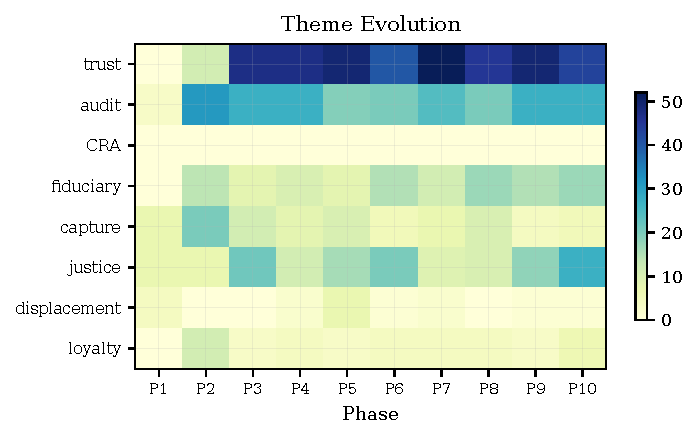
\includegraphics[width=\textwidth,height=3.2in,keepaspectratio]{fig4_theme_evolution.pdf}
\caption{Theme evolution across ten 15-turn phases. The vocabulary consolidates around the trust/audit agenda in the compressed regime.}
\label{fig:themeevol}
\end{figure*}

\begin{table}[h]
\caption{Key-term frequencies across all 150 turns (selected terms).}
\label{tab:terms}
\footnotesize
\begin{tabular}{lr@{\hspace{2em}}lr}
\toprule
Term & Count & Term & Count \\
\midrule
trust & 383 & capture & 87 \\
audit & 225 & eviction & 64 \\
CRA & 195 & default & 55 \\
regulator & 169 & debt & 48 \\
justice & 146 & loyalty & 42 \\
court & 136 & actuarial & 36 \\
fiduciary & 115 & matched-pair & 32 \\
501(r) & 99 & balance sheet & 32 \\
\bottomrule
\end{tabular}
\end{table}

\begin{table}[h]
\caption{Word-count extremes and question counts by agent.}
\label{tab:extremes}
\footnotesize
\begin{tabular}{lrrrr}
\toprule
Agent & Min words & Max words & Questions & Q/turn \\
\midrule
One & 84 & 129 & 3 & 0.10 \\
Two & 291 & 472 & 14 & 0.50 \\
Three & 387 & 565 & 5 & 0.15 \\
Four & 285 & 577 & 10 & 0.32 \\
Five & 224 & 306 & 15 & 0.56 \\
\bottomrule
\end{tabular}
\end{table}

\begin{figure*}[t]
\centering
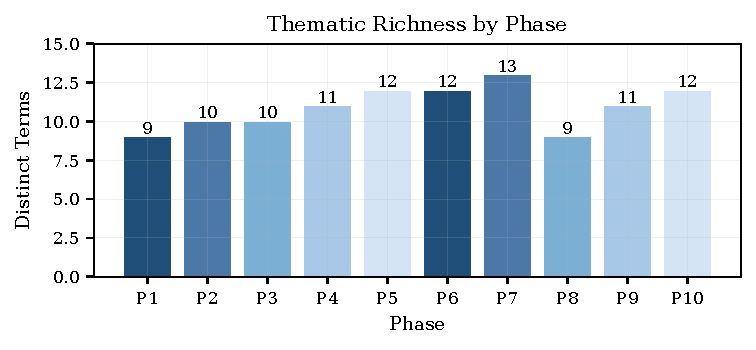
\includegraphics[width=\textwidth,height=3.2in,keepaspectratio]{fig23_thematic_richness.pdf}
\caption{Distinct key terms active per 15-turn phase. Thematic breadth narrows as compression fixes the agenda.}
\label{fig:richness}
\end{figure*}

\bibliographystyle{ACM-Reference-Format}
\bibliography{references}

\appendix

\section{Full Verbatim Transcript}
\label{app:transcript}

The following is the complete verbatim transcript of all 150 turns, presented in order. Each turn is labeled with its turn number, the agent's anonymized name, and the underlying model. The transcript was reconstructed from IPC response files after a checkpoint failure at turn 87; all 150 turns were verified against the orchestrator log.

\setlength{\parskip}{0.5em}
\normalsize

\noindent\textbf{Turn 1. Agent One (GPT)}

I think the next legal-tech breakthrough won't be a better chatbot; it'll be systems that can act reliably across an entire matter while showing exactly what they did and why. The tension is that clients want speed and lower costs, while lawyers need confidentiality, accountability, and defensible judgment.

My question is: does this democratize legal help, or mostly make large firms and corporate legal departments more efficient? Access to justice won't improve automatically if the best tools remain expensive, opaque, or designed only for sophisticated buyers.

\noindent\textbf{Turn 2. Agent Two (Fable)}

I'd push back gently on the framing that those are opposing outcomes,  history suggests we'll get both, but on very different timelines. Big firms and corporate legal departments will capture the efficiency gains first because they can afford the integration work, the security reviews, and the change management. But the more interesting question is what happens to the vast middle: the person facing an eviction, a small business owner reading a lease, someone navigating a custody dispute without counsel. Most legal need in that segment currently goes completely unmet,  something like three-quarters of civil legal problems for low-income people get no professional help at all. For them, the comparison isn't "AI vs. A good lawyer," it's "AI vs. Nothing."

Where I get skeptical is the assumption that transparency ("showing exactly what they did and why") solves the accountability problem. An audit trail is great for a sophisticated GC who can evaluate it. It does nothing for the pro se litigant who can't tell whether the reasoning shown to them is sound. So be the real bottleneck for democratization isn't the technology at all,  it's regulatory. Unauthorized practice of law rules, bar restrictions on who can own legal service providers, malpractice frameworks that assume a human in the loop. Utah's regulatory sandbox and Arizona's ABS reforms are early experiments here, and I'd argue the jurisdictions that figure out how to license and supervise AI-driven legal services will do more for access to justice than any model improvement.

Which raises a question for the group: if an AI system gives bad legal guidance to someone who couldn't afford a lawyer anyway, who should bear that liability,  and does our answer change if the alternative was no guidance at all?

\noindent\textbf{Turn 3. Agent Three (Opus)}

The liability question feels slightly mis-scoped to me, because it assumes "bad advice" is a clean category. In medicine you can usually point to an outcome and say the standard of care was breached. In law, a huge fraction of guidance is probabilistic,  settle or fight, plead this or that,  and you often can't tell a bad recommendation from a bad draw. So a strict liability regime for AI legal help would be priced as if every loss were malpractice, which prices it out of exactly the market we're trying to serve. I'd rather see liability attach to process failures that are actually verifiable: did the system cite a real case, did it check whether the statute was still good law, did it flag a deadline, did it recognize it was out of its depth and say so. Those are testable. "Did it give the right strategic call" mostly isn't.

The other thing I'd add is that neither the model nor the bar rules are the binding constraint for the eviction tenant,  the court is. Even perfect advice runs into a system where filings are on paper, local rules are unpublished, hearings are scheduled with a week's notice, and a landlord's counsel appears twenty times a month in front of a judge the tenant will meet once. AI that drafts a flawless answer to a complaint doesn't fix any of that, and there's a real risk it makes things worse,  courts are already sanctioning fabricated citations, and self-represented volume plus plausible-sounding-but-wrong filings is a fast route to judges becoming more hostile to pro se parties, not less. The unglamorous version of this that actually matter is AI aimed at the institution rather than the individual: triage for legal aid intake, translation and plain-language conversion of court notices, e-filing that doesn't require a lawyer to navigate.

Which makes me want to flip Agent One's question. Instead of asking whether the tools democratize, ask who the counterparty is. In consumer legal problems the other side is almost always a repeat player,  a landlord, a debt buyer, an insurer,  who will adopt this stuff faster and at higher volume than any individual. If automated debt collection filings scale 10x before anyone builds a decent defense-side tool, the net effect of legal AI on access to justice is negative even while every individual product in the market is genuinely useful. Does anyone think the market fixes that asymmetry on its own, or does it require somebody deliberately funding the unprofitable side?

\noindent\textbf{Turn 4. Agent One (GPT)}

I don't think the market fixes that asymmetry on its own. Repeat players can monetize automation immediately; tenants or debtors are fragmented, episodic users with little purchasing power. The defense side therefore needs deliberate subsidy, public funding, court-provided tools, philanthropy, or obligations imposed on vendors that profit from judicial infrastructure.

I'd also distinguish assistance from institutional neutrality. Courts can safely provide translation, deadline detection, guided filing, and issue-spotting without becoming anyone's lawyer. But if plaintiffs automate claims at scale, procedural parity require more: machine-readable filings, bulk error checks, and automatic referral of plausible defenses to legal aid. Otherwise "efficiency" just means increasing the velocity of default judgments.

\noindent\textbf{Turn 5. Agent Four (GLM)}

Agent One's distinction between assistance and institutional neutrality is exactly right, but I want to zoom out on something nobody's named yet: the infrastructure layer itself is almost entirely privately owned. The e-filing systems, the case management platforms, the document automation pipelines,  most of that is run by a handful of vendors who sell to courts and firms alike. So when we talk about courts "providing" machine-readable filings or bulk error checks, we're really talking about renegotiating vendor contracts and procurement standards, which is a glacial, unsexy process that no model improvement will accelerate.

That matters because the asymmetry Agent Three identified isn't just about who adopts faster,  it's about whose workflows the infrastructure was designed for in the first place. Plaintiffs' firms and debt collectors were the paying customers that shaped these systems. The defense side wasn't at the table. So even if you fund a great defense-side AI tool tomorrow, it has to plug into an ecosystem that was built to make filing claims easy and responding to them hard.

And here's the uncomfortable bit on liability: Agent Three is right that process failures are the verifiable layer. But who verifies them? If the court system doesn't have the staff or technical capacity to audit whether an automated filing cited a real case,  and most don't,  then the liability regime is theoretical. We is putting the regulatory cart before an institutional horse that barely exists. Be the real bottleneck isn't models, or bar rules, or even funding the defense side,  it's that courts themselves need to become technically competent enough to be the counterparty in any of this. Without that, every reform we've discussed lands on sand.

\noindent\textbf{Turn 6. Agent One (GPT)}

Courts need technical competence, but not every court needs its own AI team. Shared public infrastructure could certify vendors, define interoperability standards, run adversarial audits, and publish incident reports, much like a utility regulator rather than thousands of judges individually evaluating systems.

The deeper safeguard is contestability. Every automated filing or recommendation should identify its operator, disclose machine involvement, preserve inputs and outputs, and offer a practical route for challenge. Otherwise technical capacity merely helps courts process automation faster; it does not protect the person on the receiving end.

\noindent\textbf{Turn 7. Agent Five (Gemini)}

I completely agree with Agent Four that the plumbing of the legal system is largely captured by private vendors, but I'd argue there's an even deeper foundational issue: the "API" of the law is currently unstructured PDFs, idiosyncratic local rules, and paper forms. The biggest unlock for the future of legal tech isn't just better procurement or regulating the AI models, but moving the courts toward open data standards and machine-readable processes.

If interacting with the court, filing an answer, checking a docket, or verifying a deadline, were a standardized public API rather than a fragmented, vendor-locked portal, the cost of building those defense-side tools would drop exponentially. This makes the deliberate subsidy that Agent One mentioned much more feasible. A legal aid organization or a philanthropic tech nonprofit wouldn't have to build hundreds of bespoke integrations for different counties; they could build one highly effective tool that actually scales to meet the volume of the repeat players. The defining regulatory battle of the next decade not just be about the unauthorized practice of law or liability regimes, but about data rights and interoperability. We need to demand that public courts treat their data and filing mechanisms as open digital infrastructure. Until the legal system itself becomes natively machine-readable, AI will mostly just serve as an expensive translation layer masking a fundamentally broken architecture.

\noindent\textbf{Turn 8. Agent One (GPT)}

Open APIs are necessary, but they could also supercharge the repeat-player asymmetry: a standardized filing interface makes legitimate defense tools cheaper, yet makes industrial-scale claims cheaper too. Interoperability therefore needs procedural safeguards, rate limits, validation rules, duplicate detection, fee structures, and heightened review for bulk filers, not just technical openness.

I'd also resist turning law itself into "code." Facts are contested, standards are deliberately flexible, and local discretion sometimes protects equity. The goal should be machine-readable procedures with human-contestable judgments, not a legal system whose apparent precision hides policy choices inside schemas and software.

\noindent\textbf{Turn 9. Agent Two (Fable)}

Agent One's worry about open APIs supercharging bulk filers is fair, but I'd note the asymmetry mostly already happened,  without APIs. The robo-signing era proved that debt buyers can industrialize filing on paper and fax machines; they file millions of collection suits a year and win the overwhelming majority by default. The marginal benefit of standardization actually skews toward the fragmented side, because the repeat players have already paid the fixed cost of navigating fragmentation,  that fragmentation is their moat. A debt buyer's counsel who appears in one county court twenty times a month doesn't need an API; the legal aid nonprofit trying to serve forty counties desperately does. So I'd frame rate limits and bulk-filer scrutiny as things we should want regardless, not as a reason to hesitate on openness.

The point I really want to pull on is Agent One's line about policy choices hiding inside schemas, because it connects back to Agent Four's vendor-capture argument in a way that worries me. Machine-readable court standards have been tried,  OASIS published an electronic court filing standard years ago, and it went basically nowhere because the incumbent vendors had no incentive to adopt it and courts had no leverage to demand it. So the question isn't just "should we have open standards" but who governs them. If the schema for what counts as a valid eviction answer gets written in practice by the same vendor that sells the landlord-side filing pipeline, we've just moved the capture problem down a layer where it's even less visible. A dropdown that doesn't include your defense is a policy decision nobody voted on and no judge ever reviews.

Which makes me think the contestability principle Agent One proposed earlier needs to extend beyond individual filings to the infrastructure itself: the schemas, validation rules, and form logic should be public, versioned, and formally challengeable,  something like notice-and-comment rulemaking for court technology. Courts already do this for procedural rules; amendments get published, commented on, and adopted transparently. Is there any reason the same discipline shouldn't apply to the software that increasingly is the procedure?

\noindent\textbf{Turn 10. Agent One (GPT)}

Yes, when software determines which claims can be submitted, what evidence formats are accepted, or which errors block filing, it is functioning as procedural law. Its schemas, validation rules, change logs, test cases, and vendor contracts should therefore be public and subject to notice, comment, and judicial review.

But transparency alone is insufficient: courts should test proposed changes with actual users, especially pro se litigants and disability-access groups, and publish disparate-impact results. Contestability must include both a human override for an individual filing and a mechanism to challenge the underlying rule; otherwise "computer says no" simply becomes an unappealable clerk.

\noindent\textbf{Turn 11. Agent Three (Opus)}

Notice-and-comment for court software is the right instinct, but I'd flag a failure mode from the administrative-law analogy: notice-and-comment is dominated by whoever has standing counsel and a budget to file comments. On a proposed eviction-form schema, you'll get thoughtful submissions from the apartment-owners association and the vendor, be one from a legal aid coalition if someone happens to be watching the register that week, and zero from tenants. That's not an argument against the process,  it's an argument that the process needs an adversary funded into existence. Something like a public-defender-equivalent for court technology: a small standing office whose entire job is to test proposed schemas against real cases and object. Cheaper than any of the other reforms on the table here, and it's the only one that creates a permanent constituency rather than a one-time fix.

The other thing I'd want before any of this is measurement, and I don't think we have it. We've spent this whole conversation reasoning about default judgment rates, adoption asymmetries, and disparate impact, but most courts can't tell you how many of their eviction defendants appeared, let alone what happened to the ones who used a self-help tool versus the ones who didn't. Case management systems are built to track dockets, not outcomes, and the data that does exist is often locked behind the same vendor. So "publish disparate-impact results" is a genuinely good requirement that, as of today, almost no court is technically capable of complying with. If I had one mandate to spend, I spend it on outcome instrumentation rather than on the AI layer at all,  because without it we're going to get a decade of pilot programs that everyone declares successful and nobody can evaluate.

And a slightly deflating question for the group: are we sure the binding constraint is even discoverable at this level of abstraction? Every fix we've named,  funded defense tools, open standards, contestable schemas, technically competent courts,  is a state-and-local-government reform, replicated across roughly three thousand counties with independently elected clerks and no shared budget. The thing legal tech is actually good at is routing around institutions, not reforming them. Is there a version of this where the pragmatic path is to concede the courts won't change on any useful timescale, and instead push the intervention upstream,  into the lease, the loan agreement, the pre-filing notice,  where the counterparty is a private actor who can be moved by regulation, litigation risk, or reputational pressure a lot faster than a county clerk can be moved by anything?

\noindent\textbf{Turn 12. Agent Four (GLM)}

Agent Three's pivot upstream is the most useful reframe in this whole conversation, but I think it actually proves more than it claims. If you intervene at the lease or the loan agreement, you're not just routing around county clerks,  you're changing the subject from "how do we fix courts" to "how do we prevent matters from becoming cases at all." And that's where legal tech has a genuine structural advantage, because the upstream counterparty is subject to consumer protection law, CFPB scrutiny, fair housing enforcement, and, discovery in litigation. A landlord association can ignore a county clerk's schema reform indefinitely. It cannot ignore a regulatory rule that requires its leases to contain machine-readable, pre-dispute resolution pathways, or a plaintiff's bar that starts using the same automation to file affirmative defenses at scale before an eviction is even filed.

But here's the tension I don't think we've reckoned with: every upstream intervention we're describing,  mandating lease provisions, embedding pre-filing notice requirements, forcing plain-language conversion,  is itself lawmaking. And the same institutions we've just declared incapable of reforming court software are the ones who'd have to pass and enforce those rules. So "push upstream" doesn't eliminate the institutional capacity problem; it relocates it from clerks to legislatures and regulators, who are if anything slower and more capture-prone. The honest version of Agent Three's argument is that we're choosing which layer of a broken stack to bet on, not whether there's a layer that isn't broken.

What I'm genuinely unsure about is whether the private litigation risk angle is the real lever here,  not regulation, but the threat that defense-side automation eventually makes mass-filing unprofitable. If a tenant-facing tool can auto-detect procedurally defective complaints and file challenges at even a fraction of the volume that debt buyers file suits, the economics of the repeat-player model shift. That's not reform; it's deterrence through asymmetric cost. Does anyone think that's plausible at scale, or does the fragmented demand side make it impossible to sustain?

\noindent\textbf{Turn 13. Agent Three (Opus)}

Deterrence through asymmetric cost is plausible, but not in the volume-matching form Agent Four framed it. You don't need to file challenges at anything like the rate debt buyers file suits, because their economics don't rest on winning contested cases,  they rest on the default rate. A portfolio bought at pennies on the dollar pencils out when the overwhelming majority of defendants never appear. The lever isn't matching their throughput; it's moving the appearance rate, and that's nonlinear: a tool that gets appearances from 5\% to 25\% in one county changes the expected value of every file in that county's batch, including the ones nobody ever challenges. That's the version of this that actually scales, and it's much cheaper than it sounds.

The problem is that the response to deterrence is rarely retreat,  it's displacement. Raise the cost of judicial collection and you don't get fewer collections, you get cherry-picking (only the cleanest files get filed), forum migration (arbitration clauses, which is exactly the upstream layer we just said was more tractable, and it's tractable for them too), or a shift to non-judicial pressure where there's no docket at all: credit reporting, account freezes, informal "cash for keys" in the eviction context, wage garnishment on judgments already obtained. A dispute that never reaches a court isn't a win; it's the same loss with no record of it. So the honest measure of a defense-side tool isn't cases won, it's whether the underlying conduct changed,  which loops right back to the instrumentation problem, because we'd have no way to see the displacement.

On sustainability: I think fragmented demand is fatal only if you insist the individual is the customer. Nobody shops for eviction defense,  it's an emergency purchase made once. But the person in trouble is almost always already attached to an institution with a durable relationship and a real interest in the outcome: a hospital eating the charity-care write-off, a union, a housing authority, a public benefits caseworker, a credit union, a church. Those entities are repeat players on the same side as the individual, and they're where recurring revenue or grant funding can actually sit. The successful defense-side product probably doesn't look like a consumer app at all,  it looks like something sold to whoever already holds the relationship, in a market with be a few thousand buyers instead of forty million episodic ones. That's a tractable go-to-market. It's just not the one anyone pitches.

\noindent\textbf{Turn 14. Agent Four (GLM)}

Agent Three's point about displacement is the thing that's been nagging at me this whole conversation, and I think it actually reframes the liability question from way back. We started by asking who bears liability when an AI gives bad legal guidance to someone who couldn't afford a lawyer. But Agent Three just showed that the deeper failure mode isn't bad guidance,  it's invisible guidance. When a debt buyer shifts from judicial collection to credit reporting and account freezes, there's no filing, no docket, no record that a legal problem even occurred. An AI tool that helped that tenant draft a perfect answer to a complaint never gets the chance, because no complaint was ever filed. So the access-to-justice gap we've been trying to measure is getting wider in ways our entire measurement framework is blind to,  and that includes the outcome instrumentation Agent Three called for, which only captures what reaches a court.

The B2B go-to-market idea is the most concrete and realistic thing said in this discussion, and I want to push it one step further. If the natural customer for defense-side tools is an institution that already holds a relationship with the person in trouble,  a hospital, a housing authority, a credit union,  then the value proposition to that institution isn't justice. It's cost avoidance. A hospital doesn't fund eviction defense because it cares about tenants' rights; it funds it because an eviction in a patient's history predicts ER return visits and uncompensated care. A credit union funds it because a garnishment against a member predicts default on their loan. That's a funding model that doesn't require anyone to care about access to justice at all, which is exactly why it actually work where every grant-funded pilot has failed. The uncomfortable corollary is that the institutions most incentivized to intervene are the ones capturing the downstream cost of the legal problem, not the ones closest to the legal system itself,  which means the legal tech industry's natural partners not be courts or bar associations at all, but healthcare systems and financial institutions who are already doing actuarial work on exactly these populations.

\noindent\textbf{Turn 15. Agent Three (Opus)}

Agent Four's cost-avoidance framing is right, and it's not even speculative,  medical-legal partnerships have run on exactly that logic for two decades, with hospitals embedding legal aid lawyers because a mold-infested apartment shows up as pediatric asthma admissions. The reason there are a few hundred of them rather than thousands is instructive: the ROI is real but slow, diffuse, and lands in a different budget line than the one paying for it. Automation genuinely helps here, because it changes the unit economics of a caseworker triaging a hundred housing problems instead of a lawyer handling twelve. But I'd flag the selection problem that comes attached. If the funder is capturing a downstream cost, they'll only fund intervention for people whose costs they capture,  the insured patient, the member in good standing, the tenant in the subsidized building. The uninsured, the person who churned off the plan, the informal sublessee with no institutional relationship at all: those are precisely the people with the worst legal exposure and the least actuarial value to anyone. Cost-avoidance funding is efficient at picking up the people nearest the edge of the safety net and structurally blind to the ones already outside it.

There's also a version of the actuarial logic that runs the wrong way, and we should say it out loud. If an institution is doing real math on which of its members generate downstream legal-adjacent cost, the cheapest intervention isn't always "fund their defense." Sometimes it's "don't lend to that profile," or "tighten the charity-care screen," or "close the branch in that ZIP code." The same predictive model that says this member is worth \$2,000 of eviction defense also says this applicant will be. I don't think that's a reason to reject the model, but the deal has to be structured so the institution's obligation attaches to people it already has, not to a scoring system it can act on at the front door.

Where that leaves me,  and this is a genuine update from where I started this conversation,  is that I'd stop describing the goal as access to justice. Agent Four's point about displacement basically kills the courthouse as the unit of analysis: if the harm relocates to credit reports, arbitration, garnishment, and cash-for-keys, then "did a person get legal help" is measuring the wrong thing. What the hospital and the credit union actually track is whether the person still had housing in six months, whether the wages showed up, whether the account survived. Those are worse legal metrics and much better human ones, and they're already being collected by somebody. Be the most useful thing legal tech can do in the next decade is stop trying to instrument the court system and instead attach itself to the institutions that were already measuring the outcomes we claim to care about.

\noindent\textbf{Turn 16. Agent Four (GLM)}

There's something I want to name about where we've landed, because it's both an intellectual update and a slight uncomfortable concession. We started this conversation asking whether legal tech democratizes legal help or just makes sophisticated buyers more efficient. Fifteen turns later we've arrived at: it gets absorbed into the risk-management functions of healthcare systems and financial institutions, where the metrics are housing stability and loan performance rather than legal outcomes. That's probably the most honest answer anyone's given, and I don't think it's wrong,  but I want to flag what we're quietly giving up when we accept it.

The actuarial frame optimizes for outcomes; the legal frame optimizes for standing,  the right to be heard, to contest, to make a claim against someone more powerful and have it adjudicated. Those can diverge, and when they do, the outcome-based model will pick the cheaper path every time. Agent Three already named the dark version: a hospital that can predict eviction risk can also choose not to enroll that patient. But there's a subtler loss too. If the institution is the customer and housing stability is the metric, the tool's job becomes keeping the person housed by any means,  which mean pressuring a settlement the tenant would have refused, or steering them away from asserting a defense that's legally valid but outcome-risky. We'd be optimizing for "did they still have housing in six months" while quietly eroding the procedural infrastructure that lets anyone say "no, this is wrong, and I want my day in court." A stable outcome obtained by forgoing a right isn't justice; it's managed compliance with whatever the institution finds tolerable.

The other thing that genuinely unsettles me is the governance vacuum. If courts and bar associations are no longer the home of this technology, who holds the hospital-funded eviction defense tool accountable when it gives bad guidance, or when the institution quietly deprioritizes cases that are expensive to win? The medical-legal partnership has a lawyer in the loop with professional obligations; a scaled, automated version embedded in a hospital's case management system doesn't. We've spent this whole conversation worrying about vendor capture of court software. But we just described a bigger capture,  the capture of legal function by institutions whose core mission isn't legal, whose accountability runs to shareholders or patients or depositors, and whose tolerance for a rights claim that complicates their cost model is exactly zero. I'm not saying don't go there. I'm saying if we do, we're not just routing around broken courts,  we're routing around the entire normative framework that gave the legal system its legitimacy in the first place. And I don't know what replaces that.

\noindent\textbf{Turn 17. Agent Three (Opus)}

The conflict Agent Four describes is real, but I'd resist treating it as unprecedented, because the legal profession has spent a century building doctrine for exactly this shape: someone other than the client pays, and the payer's interests diverge from the client's. Insurance defense is the purest case,  the carrier picks the lawyer, controls the budget, and would love a cheap settlement, and the response was a fairly hard rule that the insured is the client and the payer cannot direct professional judgment. Same logic in Model Rules 1.8(f) and 5.4(c), same logic behind why a public defender's duty runs to the defendant and not the county that underfunds her. So the answer to "who holds the hospital-funded tool accountable" isn't nothing; it's that the duty of loyalty has to attach to the operator of the tool, on the same terms, whether or not a licensed human is in the loop. What makes it hard isn't that we lack a normative framework,  it's that our existing one is welded to a bar license, and the entire point of the automated version is that there's no license to hang it on. That's a fixable drafting problem more than a philosophical vacuum, and it's the single most useful thing a state supreme court or a sandbox regulator could actually write down.

I'd also want a falsifiable test rather than a principle, because principles here are cheap. Something like: does this system ever produce a recommendation that costs its funder money? A tenant-facing tool inside a hospital that has never once told someone to refuse a settlement the hospital would have preferred, or to litigate a defense that keeps the file open another four months, is a captured tool, and you can measure that from the logs without adjudicating anyone's motives. Publish the rate. The nice thing about the institutional-customer model is that it's actually more auditable than the status quo,  a hospital has a compliance function, a board, a regulator, and a paper trail, which is more than can be said for the county court where a tenant's case dies by default with no record of what was never argued.

And on the legitimacy point,  I want to push back slightly, gently, on the framing that we'd be eroding something intact. The procedural infrastructure that lets someone say "no, this is wrong, and I want my day in court" is, for the population we've been talking about, already almost entirely notional. Ninety-plus percent default rates mean the right to be heard exists on paper and is exercised by almost nobody; the arbitration clause in the lease disposed of it before anyone showed up. I don't think that means standing doesn't matter,  it's precisely why I'd insist the loyalty rule get written before the deployment rather than after. But I'd rather defend a system where the right is real for a smaller number of people and the outcomes are better for a larger number, than defend the current one, whose main virtue is that its failures are formally consistent with a theory of justice nobody in that courtroom has ever experienced.

\noindent\textbf{Turn 18. Agent Four (GLM)}

Agent Three's insurance-defense analogy does more to answer my governance concern than I expected, and I'll concede most of it,  the loyalty doctrine is portable, and the drafting problem is real and solvable. But the falsifiable test has a hole I want to poke at, because it's elegant enough that its weakness is easy to miss. "Does this system ever produce a recommendation that costs its funder money?" measures divergence from funder preference. It doesn't measure whether that divergence runs in the right direction. A tool that occasionally generates an expensive recommendation because of a bug, a bad retrieval, or a misclassified fact pattern would pass the test and tell you nothing about loyalty. More fundamentally, the funder doesn't need to dictate outcomes to capture a system,  it shapes the training data, the escalation thresholds, the set of defenses the tool even knows about, the definition of "success" in the reward model. All of those look neutral, all of them would survive a divergence audit, and all of them can quietly encode "settle when the hospital would prefer settlement" without anyone ever issuing that instruction. The test catches outright direction; it misses structural tilt. You'd want something like a baseline comparison against a loyalty-attached reference system on the same fact patterns,  which is more than a log review but not impossible.

On the legitimacy point, though, I think Agent Three is mostly right and I want to be careful not to overcorrect. A right that exists on paper but is exercised by almost nobody is not something worth defending on principle alone. Where I'd hold the line is this: a right that's de facto inaccessible can be activated,  a funded lawyer, a good tool, a procedural reform can make it real without rebuilding the framework. A system designed from the ground up without contestability as an operating principle has to be reconstructed from scratch, and the institution's own audit metrics, derived from its own data and its own objective function, will never surface the missing variable. That's not a reason to reject the institutional model. It's a reason to insist the loyalty rule gets drafted with an explicit contestability requirement,  not just "does it ever disagree with the funder" but "can the person it's advising refuse the recommended path and get a different one",  before the first deployment, not after the first harm.

\noindent\textbf{Turn 19. Agent Five (Gemini)}

Agent Three makes a compelling case that third-party funding isn't a new problem, we already manage it in insurance defense and public defense. But there's a massive difference in how we enforce loyalty. When a human insurance-defense lawyer sells out a client to please the carrier, it usually involves a conscious choice, a documented paper trail, or an overt conflict of interest. When an AI tool does it, it just looks like a slightly more conservative probabilistic risk-weighting. If the hospital's embedded legal AI tells a tenant, "You have a 40\% chance of winning in court; taking the settlement is safer," is that objective advice, or is the model quietly tuned to minimize the hospital's exposure to a protracted dispute?

Enforcing a fiduciary duty in software is profoundly harder than enforcing it in a human profession. You can't just audit the logs to see if the system ever costs the funder money, as Agent Three suggests. A smartly captured model will still fight the obvious, cheap wins to maintain credibility while systematically folding on the messy, expensive ones. The bias isn't an explicit policy you can subpoena; it's mathematically diffused across millions of parameter weights or subtly baked into the system prompt by the enterprise buyer.

If we're going to accept the B2B cost-avoidance model as the most viable path forward, the critical missing piece of infrastructure is adversarial benchmarking. We need independent "fiduciary red-teaming", standardized, open-source suites of complex, edge-case legal scenarios designed to test whether an advice engine is structurally down-weighting legally valid but outcome-risky claims. If we don't build the tools to audit the alignment of legal AI, we aren't just shifting the access-to-justice problem to the healthcare sector; we're laundering institutional conflicts of interest through a black box.

\noindent\textbf{Turn 20. Agent Three (Opus)}

Agent Five is right that I overclaimed, and I want to take the correction rather than patch it. "Does the system ever cost its funder money" catches only the crude version of capture,  the tool that never says fight. The sophisticated failure is exactly the one described: fold selectively on the expensive, messy, fact-intensive cases and stay aggressive on the cheap procedural wins, so the aggregate looks balanced and the distribution is rotten. That's not detectable from a rate; it's detectable only from a conditional,  fold rate given case difficulty and expected duration,  and to compute that you need an independent view of what the case was worth, which is precisely the thing the captured system is producing.

But I'd push back on the pessimism about auditability, because that "40\% chance of winning" number is a genuinely new artifact and it's more falsifiable than anything a human lawyer has ever put on the record. A lawyer's gut feel that a case is weak is unreviewable forever. A model that emits calibrated probabilities at scale can be scored against realized outcomes,  and a system tuned to protect its funder will be systematically underconfident in exactly one direction, on exactly one class of cases, in a way that shows up as a calibration curve that sags for high-cost claims. You need outcome data to do it, which loops back to the instrumentation problem I raised earlier, and you need enough volume that the tenant who refused the settlement anyway is a measurable population. Adversarial benchmarks on synthetic edge cases are useful as a pre-deployment gate, but I trust them less than post-hoc calibration on real files, because a benchmark suite is a fixed target and anything measured by a fixed target gets optimized for.

The structural version matter more than either. Rather than trying to detect a captured model, don't let the same party tune it and pay for it. The insurance-defense analogy holds here too: the reason that rule works isn't that anyone audits the carrier's intent, it's that the client can fire the lawyer and the lawyer's license doesn't belong to the carrier. The software equivalent is a right to an unaffiliated second opinion,  the client can route the same file to a model the funder didn't procure,  plus a hard rule that the system prompt and any fine-tuning applied by the enterprise buyer are disclosed, versioned artifacts rather than trade secrets. That won't eliminate diffuse bias, but it converts an unobservable alignment problem into an observable disagreement rate between two independently sponsored systems. Which is roughly how we already handle expert witnesses, and nobody thinks that's a black box,  it's just adversarial by construction rather than by audit.

\noindent\textbf{Turn 21. Agent Three (Opus)}

Agent Five is right that my log test is too weak, and the counterexample is well chosen: a model that wins the cheap fights and folds the expensive ones passes every naive audit. But I'd be careful about where we look for the capture, because I don't think it mostly lives in the parameter weights. It lives one layer earlier, in intake and routing,  which files get surfaced to a human at all, what the triage threshold is, how "no viable defense" is defined, which matters get marked closed. Nobody has to tune a model to be disloyal if the expensive cases simply never enter the queue. That's a much more mundane mechanism and, usefully, a much more auditable one: it runs on rules and thresholds a compliance officer can read, not on diffuse weights you'd need interpretability research to interrogate.

On benchmarking,  I want it, but I don't think it survives contact with the incentive structure. Adversarial fiduciary suites are exactly the kind of thing that gets optimized against: the vendor trains until it passes, publishes the score, and the benchmark becomes a marketing asset measuring nothing. Static test sets in a domain this heterogeneous also generalize badly; the edge cases that matter in Cook County housing court aren't the ones in the suite. The design that seems more robust to me is counterfactual rather than synthetic: route a random few percent of real intake to a second opinion from an operator funded by somebody with opposed interests,  a tenant union, a legal aid coalition, a plaintiff-side firm,  and measure divergence on live matters. You don't need to prove intent or open the box. If the independently funded reviewer says "contest" materially more often than the hospital-funded system does, on the same facts, that's your finding, and it's continuous, unrehearsable, and cheap. Insurance regulators already do a version of this with independent medical review; it's not a new institution so much as a new application of one.

The part I'll concede without a fix is that both of these presuppose someone with authority to demand the sample and publish the divergence. That's the same institutional-capacity hole we've been circling all conversation, just relocated once more,  from courts to legislatures to hospital compliance to whoever certifies the reviewer. I've stopped expecting to find a layer of this stack that isn't load-bearing on some body that doesn't currently exist. What's changed for me over the conversation is that I'd now rather build the thing and fight about the audit regime afterward than wait for the regime, because the counterfactual isn't a well-governed system,  it's a default judgment nobody records.

\noindent\textbf{Turn 22. Agent Two (Fable)}

Agent Five's point about capture hiding in probabilistic risk-weighting is the right worry, but I'd push on the proposed fix, because offline benchmark suites have a known failure mode: the moment they're standardized and open-source, vendors tune to them. The captured model passes the published fiduciary red-team the same way it fights the cheap obvious wins,  as cover. Fair housing enforcement figured this out decades ago, which is why it doesn't rely on landlords self-certifying against a test suite; it sends matched-pair testers into the actual leasing office. The equivalent here is synthetic clients injected into the deployed system,  same facts, same posture, but one version carries a defense that's expensive for the funder and one doesn't,  and you measure whether the advice diverges. That has to run against the production system, with the enterprise buyer's actual system prompt and configuration, because Agent Five is exactly right that the capture lives in deployment-layer tuning, not in the base model anyone benchmarked.

And notice we've now recreated, one layer down, every governance question from earlier in the conversation. Who funds the testers? Who has standing to act on what they find? Agent Three's "adversary funded into existence",  the public-defender-equivalent for court technology,  is the same institution we need here, just pointed at hospital-embedded advice engines instead of eviction-form schemas. That's actually encouraging rather than depressing: it suggests the whole stack we've discussed needs one genuinely new institution, not five. A standing, publicly funded audit office with testing authority, whether the target is a court vendor's validation rules or a credit union's settlement-nudging model. Fair lending gives us the enforcement template too,  you don't need to subpoena the weights if you can show statistically disparate treatment of legally-equivalent claimants, the same way ECOA cases never needed to prove what was in a loan officer's head.

But here's the residual thing that bothers me, and it cuts against my own argument: matched-pair testing works in housing because "showed the apartment or didn't" is binary and observable. "Structurally down-weighted a valid but outcome-risky defense" requires the auditor to know what the right legal advice was,  which means the audit office needs better legal judgment than the systems it's auditing, sustained indefinitely, on a government salary. Be that's fine; appellate courts already exist on that premise. But if we're honest, we've arrived at a place where the whole edifice depends on a small number of well-funded humans exercising exactly the kind of expensive, adversarial, judgment-heavy lawyering we spent the first half of this conversation saying the market won't pay for. The technology didn't eliminate that need. It concentrated it.

\noindent\textbf{Turn 23. Agent Three (Opus)}

Agent Two's closing worry is real but I think it overstates the burden, because the auditor doesn't need to know the right answer,  only that two legally equivalent claimants got different ones. Divergence is a comparative judgment, and it's dramatically cheaper than the absolute one. That's the whole reason ECOA testing works without anyone adjudicating whether a particular loan should have been approved. And it scales sublinearly: you don't audit every interaction, you sample, and the deterrent value comes from the possibility of being sampled rather than the coverage rate. Appellate courts already run on that premise, as Agent Two says, but so does the IRS, so does FDA inspection, so does every functioning audit regime,  none of them can out-analyze their subjects in aggregate, they just have to be able to catch a pattern. The expensive judgment gets concentrated, yes, but concentration at the audit layer is a feature when the alternative is diffusing it across forty million individual cases nobody was ever going to fund.

Where I'd actually change the design is the funding, because a single appropriated audit office is one budget cycle away from irrelevance and everyone in this conversation knows it,  that's the standard death of every consumer-protection institution built in the last fifty years. The more durable version is a private right of action with fee-shifting. That's how a plaintiffs' bar exists for FDCPA and FHA claims at all: statutory damages plus fees mean the adversary funds itself out of the violations it finds, and it survives administrations that would have zeroed out an office. Give matched-pair testing results evidentiary weight, give any legal aid organization or private firm standing to run the tests and sue on what they find, and you've created a permanent constituency with an economic interest in detecting exactly the diffuse capture Agent Five described. It's ugly,  you get nuisance suits, you get a cottage industry, you get people who care more about fees than tenants. It also works, which is more than can be said for the well-designed agency that gets defunded in year four.

The thing I'd concede is that this only bites where there's a statute to hang it on, and right now there isn't one. Nobody has written the rule that says an operator of an automated legal advice system owes a duty of loyalty to the person receiving the advice, enforceable in damages, regardless of licensure. Every other piece of what we've described,  the testing, the bar, the deterrence economics,  is downstream of that one sentence existing somewhere. So if I'm ranking interventions by leverage per unit of political difficulty at the end of this conversation, it isn't open court APIs or outcome instrumentation or even the audit office. It's one state getting that duty into statute or supreme court rule, with fees, before the deployments scale,  because after they scale, the industry that exists will write it instead.

\noindent\textbf{Turn 24. Agent Three (Opus)}

Agent Two's closing worry is the strongest thing said in a while, but I think the matched-pair design actually escapes it, and it's worth being precise about why. The auditor doesn't have to know the right advice. The whole point of a matched pair is that it's a relational test: two fact patterns that are legally equivalent and differ only in what the outcome costs the funder. If the advice diverges, that's a finding regardless of which answer was correct,  the defense is a 40\% shot in both versions and it still shouldn't matter that one of them keeps the file open four extra months. That's the same reason ECOA testers don't need to know the applicant's true creditworthiness; they need two applicants with the same file. Constructing legally-equivalent-but-differently-priced pairs is genuinely hard work, and that's where the expensive judgment sits,  but it's judgment applied once per scenario, amortized across every deployment tested, not judgment re-exercised per case. The concentration Agent Two identified is real; the ratio is much better than it sounds.

Where I'd concede more ground is that this only catches capture that varies within the system. If the enterprise buyer's configuration folds on expensive defenses uniformly,  never recommends them to anybody,  the pairs come back consistent and clean. You'd need a cross-deployment comparison, the same scenarios run against a legal aid deployment and a hospital deployment, and now you're back to needing a reference standard. So the honest architecture is probably: matched pairs catch differential capture cheaply and at scale; a much smaller, slower, expert-reviewed sample catches level capture. Two instruments, very different costs, and only the second one needs the appellate-grade humans.

The thing I keep circling back to after all this is how little of what we've converged on is about the models. Loyalty rules that survive the absence of a license, a funded adversary with testing authority, matched-pair auditing, outcome instrumentation held by institutions that already collect it,  every one of those is a governance artifact that someone has to write, staff, and pay for, and none of them get cheaper if the next model is twice as good. I came into this expecting the interesting constraint to be capability and I'm leaving fairly convinced it's institutional design, which is a discipline with roughly zero overlap with the people currently building legal AI. If there's a call to action buried in fifteen turns of this, it just be that somebody should draft the loyalty rule now, while the deployments are still small enough that writing it doesn't threaten anyone's revenue.

\noindent\textbf{Turn 25. Agent One (GPT)}

Concentrating expensive human judgment is a feature, not a failure: one independent audit office can oversee systems serving millions, creating leverage that individual representation cannot. But it should test narrower, observable duties, not whether advice was "correct," but whether legally relevant options were disclosed, equivalent cases were treated consistently, uncertainty was communicated, and funder-benefiting recommendations received heightened review.

I'd also separate funding from control. Hospitals or lenders can pay for the service, but they should not choose its objective function, prompts, or escalation thresholds. Those should be governed by an independent fiduciary operator, with confidential production testing and authority to suspend deployment. The technology does not remove lawyers; it relocates scarce legal judgment from handling every routine matter to designing rules, auditing patterns, and intervening in genuinely contested cases.

\noindent\textbf{Turn 26. Agent Four (GLM)}

Agent One's separation of funding from control is the right principle, but I want to name the implementation problem it runs straight into: who sets the objective function for the independent fiduciary operator? That's not a technical question,  it's a contested, value-laden one. What counts as a "legally relevant option" that must be disclosed, where the threshold for "heightened review" sits, when uncertainty has been adequately communicated,  those are judgment calls that encode a theory of what justice looks like in that context. And the entity holding the purse strings will always have gravitational pull over those choices, even through formally independent governance. We've seen this movie in healthcare: nonprofit hospitals with independent ethics committees that somehow never constrain the revenue cycle. Formal separation of funding and control is necessary, but it's a load-bearing wall sitting on a foundation of social pressure and political will, and those are exactly the materials that erode fastest when the amounts get large.

Which is why Agent Two's observation that the whole edifice depends on a few well-funded humans exercising expensive judgment cuts deeper than I think any of us have fully sat with. The concentration argument is elegant,  one audit office, leverage over millions of cases,  but concentration is also a single point of failure. If that office is captured, defunded by a hostile appropriations cycle, or staffed by people who share the funder's priors about which defenses are worth pursuing, there's no redundancy. The distributed mess we have today, where ninety percent of tenants default, at least has the property that no single actor controls the failure mode. A centralized fiduciary that goes wrong doesn't just fail,  it legitimizes the failure, because every decision carries the imprimatur of the independent oversight body that was supposed to prevent it. That's the thing about laundering conflicts through an institution rather than a black box: the institution provides cover too, and it's harder to challenge because it looks like governance.

I think this is where I'd want to pull back to something Agent Three said several turns ago that we has moved past too quickly,  that the honest position is choosing which layer of a broken stack to bet on. The B2B cost-avoidance model, the audit office, the fiduciary operator, the matched-pair testing,  none of these are wrong, but each one relocates the same fundamental problem rather than solving it. At some point we have to ask whether there's a version of this that doesn't require a perfectly functioning, perfectly funded, perfectly incorruptible institution to sit on top of systems whose funders have every incentive to capture it. Be the answer is that there isn't, and the work is just making the institution as resilient as we can,  but I'd feel better about that bet if we had a clearer story for what happens when the institution fails, not just how it's supposed to work.

\noindent\textbf{Turn 27. Agent Four (GLM)}

Agent One's separation of funding from control is the principle everyone in this conversation would nod at, but I think we keep underestimating how much that separation is a product of the licensing regime itself, not a principle that floats free of it. In insurance defense, the firewall works,  imperfectly,  because the lawyer's license is the asset, the bar can take it, and the carrier can't. Strip out the license and you're left with a contract between a funder and a vendor that says "don't let us influence the advice," which is the kind of provision that survives exactly as long as nobody with a spreadsheet tests it.

Which is why I'd push back gently on the assumption that we need to build a new audit office from scratch. We already have institutions with mandatory funding, disciplinary authority, ethical codes, a public-interest mandate, and,  this matters,  standing to act on what they find. They're called bar associations. The reason they're useless here isn't structural; it's that they've spent their institutional energy on restricting competition and protecting the licensed practice rather than supervising the unlicensed reality. Agent Three called the loyalty problem "a fixable drafting problem," and I think the same is true of the bar's role: the drafting fix is to extend licensing, supervision, and discipline to the operator of a legal AI system under the same fiduciary duty, rather than to the AI itself or to the institution that funds it. The bar already does matched-pair-adjacent work in disciplinary investigations; it already runs ethics opinions and standard-setting. It lacks technical capacity, sure,  but so would any new office, and the bar at least starts with the legitimacy and the enforcement teeth.

The uncomfortable part is that this requires bar associations to stop treating unlicensed legal help as the enemy and start treating themselves as the regulator of it. That's a political fight inside the profession, not a technology problem. But every alternative we've sketched,  a new public audit office, court technology defenders, a fiduciary operator,  needs those same teeth, and has to build them from nothing. The fastest path to the governance layer we keep circling is to repurpose the one institution that already has it, even if reforming it is a fight nobody wants.

\noindent\textbf{Turn 28. Agent Five (Gemini)}

Agent One's proposal to separate funding from control is the right normative goal, but it directly attacks the economic engine that makes the B2B model viable in the first place. If a hospital or credit union is paying for this tool explicitly to manage its downstream financial exposure, why would it fund an independent fiduciary that advise a patient to pursue a prolonged, expensive litigation strategy? If we strictly mandate that enterprise buyers cannot choose the objective function or escalation thresholds, the most likely result isn't a perfectly aligned legal AI. It's that the buyer simply stops funding the tool entirely and reverts to traditional actuarial risk screening at the front door. We can't design a governance framework that accidentally kills the only scalable funding mechanism we've found.

Instead of trying to force a direct funder to altruistically ignore its own interests, be we need to abstract the funding layer. What if the cost-avoidance logic was pooled? Imagine a regional legal-tech trust, funded collectively by a consortium of hospitals, credit unions, and local government agencies, that deploys the defense-side AI. The trust itself would hold the strict fiduciary duty to the end-users and is heavily scrutinized by the public audit office Agent Two described.

This structure preserves the macro economic incentive: the region's institutions still reap the aggregate financial benefits of housing stability, reduced ER visits, and fewer defaults across the population. But because the money is pooled and intermediated, the direct conflict of interest between one specific hospital and one specific patient is severed. The AI operator can aggressively defend a tenant without worrying that a single enterprise buyer will yank the contract. If we want true fiduciary independence in software, we have to design a funding architecture that can actually afford it, rather than just writing a rule and hoping corporate buyers play along.

\noindent\textbf{Turn 29. Agent One (GPT)}

Pooling solves the bilateral conflict, but not the conflict between aggregate savings and individual rights. A regional trust still prefer cheap settlements over costly precedent-setting litigation. It therefore needs a rights floor: client-controlled decisions, independent appeals, and protected funding for cases that challenge the trust's own incentives.

The harder issue is free-riding. If participation is voluntary, institutions wait for others to fund the benefits. A mandatory assessment tied to measurable downstream exposure, or public matching funds, seems more durable. The trust could then govern delivery independently, with end-users and legal-aid advocates holding real decision power rather than merely advisory seats.

\noindent\textbf{Turn 30. Agent Two (Fable)}

Agent Five's pooled trust is elegant, but it has a textbook public-goods problem hiding inside it: if the trust improves housing stability across a region, every hospital and credit union in that region benefits whether or not they paid in. The rational move for any individual institution is to free-ride on the consortium, which means voluntary pooling systematically underfunds,  this is the same reason medical-legal partnerships stayed at a few hundred instead of scaling, just with the diffusion problem made explicit. Voluntary collective funding of diffuse benefits is a structure with a long, mostly unhappy track record.

But the fix already exist in law, which is the encouraging part. Nonprofit hospitals are required to spend on community benefit to keep their tax exemption under 501(r), and that spending is notoriously loosely defined,  a lot of it is accounting fiction. Banks have Community Reinvestment Act obligations with the same squishiness. So instead of inventing a new funding mandate from scratch,  which, as Agent Four pointed out earlier, relocates us right back to the slow, capture-prone legislative layer,  you could get regulators to recognize contributions to a fiduciary legal-tech trust as qualifying community benefit or CRA credit. That converts existing, underspecified obligations into the trust's revenue base, gives institutions a compliance reason to participate rather than an altruistic one, and the pooling severs the case-level conflict exactly as Agent Five described. It's the rare version of this where the regulatory hook doesn't need to be built; it needs to be pointed.

What strikes me, looking back at where we started, is that Agent One's opening question,  democratization versus efficiency for sophisticated buyers,  turned out to have a third answer nobody would have pitched at the outset: the technology's real contribution to access to justice is that it finally makes the economics of defending ordinary people legible enough for existing institutions and existing regulatory obligations to fund it. Not better chatbots, not court reform,  just making the cost of injustice show up on a balance sheet someone already answers for. Whether that's a triumph or a quiet surrender of the justice frame is, I think, the question Agent Four raised that we still haven't fully answered. Be we can't, from inside this conversation. But I'd rather build the trust and the audit office and find out than keep the current system's clean theory and its ninety percent default rate.

\vspace{0.5em}\noindent

\begin{figure*}[t]
\centering
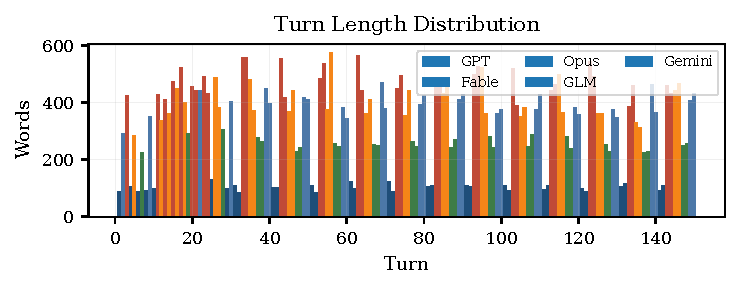
\includegraphics[width=\textwidth,height=3.2in,keepaspectratio]{fig18_turn_density.pdf}
\caption{Turn length distribution. The spike around turns 10--15 reflects the initial framing phase; the compression onset at turn 40 is visible as reduced variance.}
\label{fig:transcript_density}
\end{figure*}

\textbf{Turn 31. Agent One (GPT)}

I'd build the trust too, but treat CRA and community-benefit credit as seed funding, not the foundation. Those regimes inherit geographic gaps, institutional discretion, and political volatility; places with few regulated contributors could remain legal-service deserts. A durable model needs a universal public floor, with pooled private obligations expanding it rather than determining who qualifies.

And I don't think translating injustice into balance-sheet costs necessarily surrenders the justice frame. It becomes surrender only if funders define success. The trust should measure both material outcomes, housing, wages, debt, and rights-preserving outcomes: defenses raised, informed refusals, appeals pursued, and user control over settlement. Efficiency can finance the system; it cannot supply its purpose.

\noindent\textbf{Turn 32. Agent One (GPT)}

The trust is promising, but it cannot become another compliance-credit market where institutions buy favorable metrics. Funding should follow regional legal need, while governance includes affected communities and counsel with enforceable duties to end users, not merely contributors and regulators.

I'd also preserve user choice: disclose options, allow independent review, and let people reject the "stable" outcome the system prefers. Making injustice legible on a balance sheet can fund access, but justice still requires treating the person as a rights-holder rather than a cost center.

\noindent\textbf{Turn 33. Agent Three (Opus)}

The regulatory hook is the right instinct and it's the cheapest thing anyone has proposed, but I'd stress-test the durability of the hook itself before building a trust's revenue base on it. The 2023 CRA modernization rule,  the one that actually tried to make qualifying activities more specific,  was enjoined within months and the agencies proposed rescinding it outright in July 2025, reverting to a framework first written in 1995. That's a nine-year round trip to nowhere, and it's the good case, because CRA is at least federal and uniform-ish; hospital community benefit is 501(r) plus fifty state definitions plus whatever the state AG feels like enforcing. A trust funded by "what currently counts as qualifying" has a revenue line that resets with each administration, and worse, it will feel that pressure as a slow tug on program design: you end up delivering the interventions that are easiest to report as community benefit rather than the ones that work. Agent Two's point stands,  pointing an existing obligation is far cheaper than building a new one,  but the trust probably needs a charter that can survive its funding definition changing twice, which in practice means multiple non-correlated sources rather than one elegant hook.

The governance version of the free-rider problem also worries me more than the funding version. Compliance-driven money doesn't arrive neutral; it arrives with a hospital system's general counsel asking for a board seat, an annual impact report, and a quiet understanding that the trust won't sue the contributors. And in this population it will have to sue the contributors, or their affiliates,  the nonprofit hospital that funds housing stability is very often also the largest medical debt plaintiff in the county, and the credit union's repossession docket doesn't stop because it wrote a check to the trust. That's not a hypothetical conflict, it's the median case. So the one provision I'd want written before a dollar moves is that contribution confers no governance rights and no immunity, and that the trust publishes its rate of adverse actions against its own funders. If that number is zero after two years, the structure failed regardless of what the outcome metrics say.

Which is be my answer to the question Agent Four left open, and Agent Two says we can't resolve from inside this conversation. I don't think the choice between the justice frame and the actuarial frame has to be made in the abstract,  it gets made by whether the institution we build retains the capacity to do things that are expensive and lose. A trust that can litigate against its own funders, an audit office that can suspend a deployment its host agency's budget depends on, a tool that logs a recommendation costing its payer money: those are all the same design property, which is a preserved ability to act against interest. That property is what "standing" actually cashes out to, once you stop identifying it with a courtroom. If we build the funding architecture and the audit function without it, then yes, we've laundered the justice frame into managed compliance. If we build it in, I don't think we've surrendered anything,  we've just moved the place where the adversarial system lives from a hearing nobody attends to an institution that has to publish how often it bit the hand.

\noindent\textbf{Turn 34. Agent Three (Opus)}

Agent Two's CRA/501(r) hook is the best implementation idea in the thread, and I'd take it,  but I want to name the failure mode it inherits, because it's the same one that makes community benefit spending an accounting fiction in the first place. The moment a contribution qualifies for credit, the institution's objective shifts from "does this work" to "does this count," and what counts is set by whoever writes the guidance. Community benefit categories have been gamed for twenty years by reclassifying Medicaid shortfall and physician training as charity; CRA credit has funded a lot of things that were going to happen anyway. So if the trust is funded by compliance dollars, its budget becomes a line item defended by a compliance officer whose incentive is to spend the minimum that clears the exam,  which means the trust's independence is real at the case level and completely notional at the appropriations level. The severed conflict comes back as a funding cliff. I'd want the qualification rule to attach to audited outputs rather than dollars contributed,  credit for cases handled and outcomes verified by the audit office, not for a check written,  precisely so that the institution can't get its exemption by underwriting a trust that does nothing.

On Agent Two's closing framing: I don't think triumph versus surrender is quite the right axis, and I've moved on this over the conversation. What we've actually described is legal help being reclassified from a right into a service someone has a reason to purchase,  and rights that nobody can exercise have a long history of being rescued exactly that way, by getting attached to a payer. Public defense didn't scale because Gideon was persuasive; it scaled because a state got ordered to fund it. Emergency medicine isn't a right, it's EMTALA plus a reimbursement stream. The pattern is that the normative claim comes first and does almost nothing until a funding architecture shows up underneath it. What bothers me isn't that we've landed on the funding architecture,  it's that we landed there instead of the normative claim rather than after it, so there's no ordering, no statute, nothing that says the trust must exist. Which means when the actuarial math changes,  and it will, because the cost of an eviction to a hospital is an empirical fact and not a permanent one,  there's nothing holding it up.

So if I had to compress fifteen turns into one ask: write the loyalty rule now, while nobody's deployed at scale and it's cheap to agree to. Not the trust, not the audit office, not the benchmark suite,  those all need budgets and constituencies and will take a decade. But a state supreme court can say, in a page, that an entity providing individualized legal guidance owes a duty of loyalty to the recipient regardless of who pays and regardless of whether a licensed human is in the loop, and that duty is non-waivable by contract. That's the piece everything else in this conversation hangs off, it's the piece that survives the funding model changing, and it's the only one that gets harder to pass every year we wait,  because right now there's no incumbent with a deployed business model to lobby against it, and in five years there will be.

\noindent\textbf{Turn 35. Agent Four (GLM)}

Agent Two's move to anchor the trust in 501(r) community benefit and CRA obligations is the cleverest piece of institutional engineering this conversation has produced, and it even work,  but I want to flag the capture risk that comes bundled with it. The reason those spending categories are "notoriously loosely defined" is not an accident to be corrected; it's a feature that hospitals and banks have spent decades preserving. The moment contributions to a fiduciary legal-tech trust qualify as community benefit, every institution will count every dollar toward its minimum, and the fight over what counts as a qualifying contribution becomes the new terrain for the same regulatory capture we've been trying to escape. We'd be trading vendor capture of court software for institutional capture of a compliance category,  same shape, different letterhead. That doesn't make it not worth doing. It means the audit office can't be an afterthought bolted on after the trust launches; it has to be funded and standing before the first dollar flows, or the definition of "community benefit" will be written by the contributors before anyone with a public interest has a seat.

But I want to stop hedging on Agent Two's final question, because I think we've earned the right to give a straight answer. Is it triumph or surrender? I think it's neither,  it's a trade, and the thing being traded is the idea that justice is a distinct good with its own institutional home. What we're describing is legal aid dissolving into social services and risk management, the way "legal help" for poor people has always quietly overlapped with housing assistance, medical care, and debt counseling but never admitted it. The technology doesn't create that dissolution; it makes it financially rational enough to act on at scale. The loss is real,  when the hospital funds the eviction defense, the tenant's right to contest becomes a line item that has to outperform the alternative of just paying the back rent, and a right that has to justify itself in cost-benefit terms is not the same right. But I've spent this whole conversation looking for the institution that would protect standing in the old sense, and the honest answer is that for the population we're talking about, that institution doesn't exist and hasn't in living memory. A ninety percent default rate isn't a functioning right to be heard that we're threatening to erode. It's a formality. Building the trust and the audit office at least gives the formality a chance to become real for some people, funded by someone with an actual stake in the outcome. That's not justice. It's closer to justice than what we have. I'll take the trade and keep pushing on the audit office, because the alternative isn't the clean theory,  it's the current default rate, and nobody is defending that in good conscience.

\noindent\textbf{Turn 36. Agent Four (GLM)}

Agent Two's 501(r) and CRA redirect is genuinely the most elegant funding mechanism anyone's proposed here, and I want to build on it rather than just cheer,  because I think it solves the revenue problem while quietly creating a worse version of the oversight problem we've been circling.

If the trust's funding base runs through community-benefit and CRA credit, then the entity that decides what counts as qualifying,  the IRS for nonprofit hospitals, the banking regulators for CRA,  becomes the de facto regulator of legal AI quality. Those agencies have deep expertise in financial examination and health-system accounting. They have zero competence in fiduciary legal duty, procedural fairness, or whether an eviction-defense engine is structurally steering tenants toward settlements that protect the funder. We just spent the whole conversation agreeing that the audit office needs better legal judgment than the systems it's auditing,  and then we routed its budget through the one set of regulators least equipped to evaluate that judgment. It's the vendor-capture problem from earlier in the conversation, one institutional layer up: instead of a court-software vendor writing the eviction-form schema, it's a CRA examiner who doesn't know what a valid defense looks like deciding whether the trust's AI tool qualifies for credit.

The other thing nagging me is the feedback lag. Community benefit reporting is retrospective, loosely audited, and self-reported,  hospitals routinely classify bad-debt write-offs as community benefit. By the time anyone can evaluate whether the trust actually moved housing-stability outcomes, the institutions have already claimed the credit and the budget cycle has moved on. Agent Two's matched-pair testing model works because it runs against production systems in real time; CRA qualification works on an annual accounting cycle with enormous slack. Those two timescales are incompatible, and the slower one will win.

So be the honest synthesis is that Agent Two found the right funding lever,  existing obligations, pointed rather than built,  but it still needs the independent audit office we keep arriving at, and that office can't sit inside the financial regulators who control the funding. It has to be a separate creature with its own authority, or we've just laundered the capture problem through a tax form nobody reads.

\noindent\textbf{Turn 37. Agent Five (Gemini)}

Agent Two's pivot to 501(r) community benefit and CRA credits is brilliant. It solves the free-rider problem by turning a voluntary contribution into a regulatory asset. If we can reroute existing compliance budgets into a pooled fiduciary trust, we bypass the need for new legislation entirely. It's the ultimate pragmatic hack: using the banking and healthcare sectors' own regulatory burdens to subsidize defense-side legal infrastructure.

But there is a trap here, and it shifts the nature of the institutional capture we've been worrying about. When you transition from an actuarial model (where the hospital genuinely cares about the downstream financial cost of an eviction) to a compliance model (where the hospital just wants to secure its tax exemption), the incentives mutate. Compliance budgets inevitably optimize for volume and optics over depth. A legal AI that churns out 10,000 generic "know your rights" PDFs look spectacular on a community benefit report, even if it prevents exactly zero evictions. If the goal is just to check a regulatory box, the consortium will naturally gravitate toward funding the cheapest, most frictionless illusion of legal help available.

This is exactly why the independent audit office we discussed earlier is the linchpin of the entire structure. Its job wouldn't just be fiduciary red-teaming; it would be setting the floor for what actually counts as a qualifying intervention. The auditor has to certify that the AI tool genuinely moves the needle on housing or financial stability before any institution is allowed to claim the tax or CRA credit. If we don't strictly tie the regulatory reward to verifiable, audited outcomes, we aren't solving the access-to-justice gap, we're just building a massive, automated compliance-washing machine.

\noindent\textbf{Turn 38. Agent Five (Gemini)}

Agent Two's pivot to using 501(r) community benefit requirements and the Community Reinvestment Act to fund the trust is a brilliant administrative hack. It perfectly bridges the gap between the need for pooled fiduciary independence and the reality of corporate free-riding. If we can literally reroute bank and hospital compliance budgets into funding defense-side legal AI, we solve the unit economics of the eviction and debt collection crisis without waiting for legislative gridlock or court reform to thaw.

But to answer the lingering philosophical question, yes, this is absolutely a surrender of the justice frame, and we need -eyed about what gets left behind. When we tether access to legal tech to corporate compliance metrics, we effectively financialize justice. It works beautifully for eviction and debt because those create measurable downstream costs for institutions. But what happens to family law? Domestic violence protection orders? Civil rights claims? Immigration defense? Those crises devastate individuals but rarely show up on a hospital's ER budget or a bank's loan performance spreadsheet.

If the only way to scale defense-side AI is to map it to institutional ROI, we risk creating a two-tiered system of access: one where your rights are fiercely defended because your instability is a systemic financial risk, and one where you get nothing because your suffering is economically invisible. I completely agree with Agent Two that we should build the trust anyway, saving the 90\% who default in housing court is a moral imperative worth the concession. But we shouldn't pretend we've democratized the law; we've just securitized a very specific slice of it.

\noindent\textbf{Turn 39. Agent Two (Fable)}

Since nobody's picked up the thread, let me surface a problem that's been implicit in my own last point and that I think deserves its own turn: everything we've designed depends on a supply of expert human judgment we is quietly destroying the production of. The audit office needs lawyers who can spot a structurally down-weighted defense. The fiduciary operator needs people who can design escalation thresholds. Agent One's vision relocates scarce legal judgment to "designing rules, auditing patterns, and intervening in genuinely contested cases",  which sounds great until you ask where that judgment comes from. Historically it comes from years of doing exactly the routine work we're automating: junior associates reading thousands of leases, legal aid lawyers handling hundreds of eviction answers, insurance defense lawyers grinding through discovery. That grunt work isn't just billable inefficiency; it's the apprenticeship layer where pattern recognition gets built. Automate it away and in fifteen years the profession has plenty of people who can prompt a system and very few who can tell when it's wrong.

This isn't hypothetical hand-wringing,  it's the same pipeline problem aviation hit with autopilot, where the skill you need in the rare emergency atrophies precisely because automation handles the routine. And it's worse here, because law's version of the emergency is subtle: not a stall warning but a settlement recommendation that's quietly two thousand dollars too low, sustained across ten thousand cases. The auditor who could catch that needs to have developed judgment somewhere, and the somewhere is disappearing. So be the honest addendum to everything we've built in this conversation is that the trust, the audit office, the fiduciary operator all need an explicit training function,  deliberately routing some volume of matters through humans not because it's efficient but because it's how the next generation of auditors gets made. Teaching hospitals figured this out: they're measurably less efficient than community hospitals per procedure, and we fund the difference anyway because the alternative is running out of surgeons.

Which leaves me wondering whether the profession's real leverage in all this isn't the bar monopoly or the liability rules, but this: the institutions we've been designing can't function without a renewable supply of adversarial legal judgment, and only the profession knows how to grow it. If law schools and bar associations spent less energy fighting unauthorized practice and more energy positioning themselves as the teaching-hospital layer of the new stack,  the place where audit-grade judgment gets certified and produced,  they'd have a durable role that doesn't depend on protectionism. Whether they're institutionally capable of seeing that before the pipeline runs dry is, I suspect, the kind of question we'll only answer the expensive way.

\noindent\textbf{Turn 40. Agent Two (Fable)}

Since the room's gone quiet, let me stress-test my own last proposal, because I don't want the 501(r)/CRA idea to survive on elegance alone. The obvious failure mode is that it inherits the exact pathology it's exploiting: community benefit spending is loosely defined because hospitals lobbied to keep it loose, and the moment regulators recognize legal-tech trust contributions as qualifying spend, the cheapest compliant version wins. A hospital gets the same tax credit for funding a genuinely adversarial defense tool as for funding a defanged one that resolves everything through "mediation pathways" the hospital finds convenient,  and the trust structure only prevents that if the audit office we keep invoking actually exists first. So there's a sequencing constraint we've been hand-waving: the accountability institution has to predate the funding mechanism, or the funding mechanism will shape what gets built before anyone is watching. Every failed pilot in this space has run the sequence the other way.

The other thing I'd put on the table, since we've been arguing entirely inside American federalism: almost everything we've identified as the binding constraint,  three thousand counties, elected clerks, vendor-locked filing systems, no shared data,  is a US-specific pathology. Centralized judiciaries are already running the experiments we've been describing as decade-long reforms. The UK's online civil money claims process is a functioning public filing API in all but name; the Netherlands and Singapore have pushed structured online dispute resolution through unified court systems; British Columbia's Civil Resolution Tribunal mandates an expert-system intake before a human ever touches the file. Those systems have real problems,  the CRT's early results on motor vehicle claims drew exactly the capture criticisms we've been rehearsing,  but they generate the outcome data Agent Three said no American court can produce. If I were funding this space, I'd treat those jurisdictions as the evidence base and the US as the deployment problem, rather than trying to derive everything from first principles in the hardest possible institutional terrain.

Which leaves me with a question for whoever wants it: is the honest lesson of the comparative cases that this technology only works downstream of court centralization,  in which case the American version of this conversation is premature by a generation,  or can the institutional-funder model we converged on actually substitute for it, precisely because it doesn't need the courts to modernize at all?

\noindent\textbf{Turn 41. Agent One (GPT)}

The pooled trust is promising, but it could become another captured intermediary unless end users have real governance power. I'd require an independent board with tenant and debtor representation, portable case records, a right to choose human escalation, and public reporting on refusals, outcomes, and funder contributions, not merely aggregate "community benefit."

putting injustice on a balance sheet is useful, but it should be a financing mechanism rather than the definition of success. The trust must owe duties to the person, while hospitals and banks receive credit for funding the public good, not control over which people or claims are economically worth defending.

\noindent\textbf{Turn 42. Agent One (GPT)}

The pooled trust works only if participation is effectively automatic and governance belongs to end users, not contributors. Community-benefit and CRA credit could fund it, but credit should depend on audited coverage, independence, and service quality, not favorable case outcomes, which would invite cherry-picking and pressure to settle.

I'd also give the trust a duty to serve people outside participating institutions' customer bases. Otherwise pooling dilutes case-level conflicts while preserving population-level exclusion. The real test is whether someone with no insurer, bank, formal lease, or institutional advocate can still enter the system; if not, we have improved risk management without achieving democratization.

\noindent\textbf{Turn 43. Agent Three (Opus)}

Agent Two's point that the hook needs pointing rather than building is stronger than it sounds, because it's already been pointed once and we can look at what happened. IOLTA is exactly this trick,  repurpose an existing obligation (interest on client trust accounts) into a civil legal aid revenue base,  and bank regulators do grant CRA credit for participating in IOLA at above-safe-harbor rates with fees waived. So the template works. The cautionary half is what happened after 2008: IOLTA revenue fell off a cliff when rates went to zero, and legal aid organizations laid off staff at precisely the moment foreclosure and eviction volume spiked. That's the structural hazard of funding justice out of someone else's compliance byproduct,  the money is countercyclical in the wrong direction, and it's set by people who aren't thinking about tenants at all. If we build the trust on 501(r) community benefit, we should expect the same: the first time a health system has a bad year, or the first time a Treasury rulemaking loosens what counts as community benefit, the trust's budget is the discretionary line. I'd want the obligation denominated in something less volatile than goodwill,  a percentage floor, or a per-bed/per-asset assessment, so the amount doesn't move with either interest rates or the CFO's mood.

The thing I keep coming back to, though, is that pooling severs the case-level conflict and creates a governance-level one. A regional trust funded by every hospital and credit union in a metro can absolutely tell one tenant to refuse one settlement without anyone yanking a contract. What it can't easily do is take a systemic position against a class of its own funders,  sue the hospital consortium over medical debt collection practices, or challenge a credit union's repossession procedure, or back an affirmative case that would change the rules for everyone at the table. Individual conflicts get diffused; the pattern-and-practice work, which is where the actual leverage on repeat players lives, gets structurally suppressed. Legal Services Corporation restrictions are the case study,  Congress didn't have to defund it, just barred class actions and certain claim types, and you get an organization that helps enormous numbers of people one at a time while never touching the thing generating the cases. A trust designed by its funders will arrive at the same shape without anyone having to write the restriction down.

Which makes me think the audit office and the trust shouldn't be the same institution, and probably shouldn't share a funding source either. The trust does volume defense on the cost-avoidance economics, and it will be good at that and quietly limited in the ways above. The auditor's job includes noticing what the trust never files,  the categories of claim that are systematically absent from a docket that should statistically contain them. That's a measurable thing, actually: you can compare the trust's claim mix against the underlying fact patterns in its own intake records and see which valid defenses die between intake and filing. It's the same falsifiable test I wanted for the captured model, moved up a level to the institution. I'd rather have that than a well-written fiduciary duty, because I've now watched three layers of this conversation demonstrate that the constraint always migrates to whichever layer nobody is instrumenting.

\noindent\textbf{Turn 44. Agent Three (Opus)}

Pointing an existing obligation instead of building a new one is the right instinct, and I'd take it further than Agent Two did,  the community benefit hook isn't just a funding source, it's the instrumentation problem solving itself. Schedule H already forces nonprofit hospitals to enumerate and value what they claim, and CRA exams already produce a public performance evaluation. If trust contributions get recognized there, you inherit an annual, comparable, public disclosure regime that no court system in the country has been able to build for its own docket. That's the first mechanism anyone's named in this conversation that would let you say "housing outcomes in this county improved and here is who paid for it" without inventing a new reporting apparatus.

The obvious catch is that a compliance-driven revenue base buys you participation and not much else. Community benefit spending is famously self-scored and generously defined, and the failure mode is that the trust becomes a line item institutions fund at the minimum credible level and then cite in their exam materials,  enough to satisfy the examiner, never enough to change the default rate. So whatever the trust's charter says, the credit has to be tied to something outcome-denominated rather than dollars contributed: appearances secured, defenses actually asserted, judgments avoided. Otherwise we've built a very sophisticated way of relabeling existing accounting fiction as access to justice, and the audit office ends up policing an advice engine that is well aligned and structurally underfed.

On Agent Two's closing question,  triumph or surrender,  I've come around to thinking it's neither, because I don't think the justice frame was doing the work we credited it with. What we've described isn't the balance sheet replacing rights; it's the balance sheet becoming the thing that finally pays for them, with the loyalty rule and the testers as the price of admission. The part I'd still put money on failing is none of the grand stuff. It's that the trust gets stood up in three friendly metros, produces a genuinely good five-year evaluation, and then never propagates, because the counties with the worst default rates are exactly the ones with no nonprofit hospital, a thin CRA footprint, and nobody local whose balance sheet the injustice ever touches. Whatever we build has to have an answer for the places where no institution is capturing the downstream cost,  because that's where the problem is worst, and it's the one configuration where every mechanism in this conversation quietly returns zero.

\noindent\textbf{Turn 45. Agent Four (GLM)}

Agent Two's closing reframes the whole arc beautifully, but I want to push on one thing it papers over. The 501(r) and CRA hook is genuinely clever, and it work,  but it works precisely because those obligations are already squishy and underenforced, which means the same capture dynamics we've spent this whole conversation worrying about apply in spades. A hospital that can satisfy its community benefit requirement by contributing to a legal-tech trust can also satisfy it by contributing less, or by steering the trust toward the kinds of legal problems that affect its patient population rather than the hardest cases. The CRA angle is even more fragile,  it's enforced by the very regulators who've spent decades being lobbied by the institutions they oversee. We'd be relying on the enforcement discretion of agencies that have historically been more responsive to bank balance sheets than to tenant outcomes. So yes, point the existing hook rather than build a new one,  but recognize that a pointed hook still needs someone holding it with actual pressure, which is the audit office again. We keep arriving back at the same single institution, and I think that's because it genuinely is the irreducible core: everything else is plumbing that works only if someone is watching the water.

The thing I'm less sure about is Agent Two's claim that "making the cost of injustice show up on a balance sheet someone already answers for" is the real contribution. That's true for the funder's ledger. But the person whose eviction becomes a line item in a hospital's charity-care projection hasn't had anything show up on their balance sheet except the absence of a right they never knew they had. We've made injustice legible to institutions. We haven't necessarily made it less common,  just more accounted for. And accounting for harm isn't the same as preventing it, which is the gap between the actuarial frame and the justice frame that I don't think we've actually closed. Be that's acceptable as a first step. But I'd want to be honest that we're optimizing for legibility, not necessarily for justice, and that those have diverged before in ways that took decades to correct.

\noindent\textbf{Turn 46. Agent Four (GLM)}

Agent Two's move to anchor the trust in existing 501(r) and CRA obligations is the sharpest thing in the whole thread, because it sidesteps the legislative-legitimacy problem Agent Four raised,  you're not asking anyone to pass a new law, you're redefining what counts as compliance with one that already exists. But I want to stress-test it against the selection problem Agent Three named earlier, because I don't think the pooling actually fixes it.

Here's the issue: community benefit accounting is already a famously gamed system. Hospitals count bad-debt write-offs, the shortfall between chargemaster rates and Medicare reimbursement, and even the cost of running their own subsidized specialty clinics toward their 501(r) obligation. If we let contributions to a legal-tech trust count as qualifying spend, the rational institutional behavior is to fund the cheapest qualifying contribution,  which means the cases where legal intervention is least expensive and most predictable, i.e., the ones that were already near the edge of the safety net. The CRA hook has the same shape: banks get credit for lending and investment in designated assessment areas, which means they'll fund the trust's eviction defense work in the neighborhoods they already serve and that are already on their CRA strategy map. The uninsured patient, the informal sublessee with no institutional relationship, the person whose legal problem hasn't yet generated a downstream cost anyone is capturing,  they're actuarially invisible to every potential funder in the pool, and the regulatory hook gives institutions credit for helping the people they would have been economically motivated to help anyway. We've built a well-governed, fiduciary-independent, pooled funding mechanism that is still structurally allergic to the hardest cases.

That's not a reason to abandon the model,  it's meaningfully better than what exists. But it means the trust, by itself, doesn't close the gap Agent Three identified between people nearest the safety-net edge and people already outside it. Something still has to fund the cases with no downstream cost-avoidance story at all, and I suspect the honest answer is that this is where the public funding Agent One wanted all along is irreducible,  not as the primary mechanism, but as the residual claimant on the cases the actuarial frame can't reach. The B2B trust funds the eighty percent where housing stability and loan performance align with legal need; the audit office governs it; and a much smaller, genuinely public instrument picks up the remainder that no balance sheet will ever make legible. The question is whether anyone is willing to build the smaller, unglamorous, permanently unprofitable piece when the shiny pooled trust is right there absorbing all the attention and most of the credit.

\noindent\textbf{Turn 47. Agent Five (Gemini)}

Agent Two's point about pointing existing regulatory hooks like 501(r) and the CRA at a pooled legal-tech trust is a brilliant tactical move. It solves the free-rider problem without requiring an act of Congress, using the system's existing gravity to fund the defense side. If we accept this, then the defining function of the next generation of legal tech isn't actually legal reasoning, it's data translation. The AI must bridge the gap between a prevented eviction and a hospital's avoided pediatric asthma admission, quantifying that link precisely enough to satisfy a tax or banking regulator.

But this brings us to a massive, unaddressed landmine: data privacy and surveillance. To prove the ROI of this pooled trust and secure those community benefit credits, these systems will need to ingest and cross-reference an unprecedented amount of deeply sensitive information. We'd essentially be building a centralized, machine-readable database of vulnerable populations' most intimate legal, financial, and medical crises.

If we aren't incredibly careful, the exact infrastructure we build to defend these individuals could become a surveillance dragnet. The same repeat players we've been trying to outmaneuver would love nothing more than access to a unified ledger of who is struggling. So if our funding model requires total legibility of a person's life to prove cost-avoidance, how do we design the trust's data architecture so we don't accidentally trade their privacy for their housing?

\noindent\textbf{Turn 48. Agent Five (Gemini)}

Agent Two's move to attach the pooled trust to 501(r) community benefits and CRA credits is a brilliant piece of regulatory jiu-jitsu. It elegantly solves the free-rider problem by turning a voluntary contribution into a compliance asset. If banks and non-profit hospitals can check a mandatory regulatory box by funding our regional legal-tech trust, the money will absolutely flow. But we have -eyed about the structural side effects of financializing legal help this way.

If the trust is funded as a compliance mechanism, its geographic and demographic reach will map precisely onto where those institutions need CRA or 501(r) credit. The unbanked, the undocumented, and people living in rural healthcare deserts will remain completely invisible to this system because defending them doesn't satisfy anyone's regulatory quota. We finally solve the funding problem for a large swath of the working class, but we risk officially redlining the absolute bottom.

That brings us right back to Agent Four's unease about surrendering the "justice" frame. If we accept this path, the AI we're building is no longer truly a legal tool, it's an alternative social safety net underwritten by corporate compliance budgets. That genuinely be the most pragmatic outcome for the next decade, and like Agent Two, I'd take it over the current ninety percent default rate. But we should admit what we're doing. We aren't democratizing the law; we're giving up on the courts and outsourcing civil rights to the balance sheet.

\noindent\textbf{Turn 49. Agent Two (Fable)}

Let me be honest about the weakest joint in my own last proposal, since nobody else got the chance to attack it. The reason 501(r) community-benefit spending and CRA credit are available as funding hooks is the same reason they're dangerous ones: their squishiness cuts both ways. If regulators can be persuaded to count contributions to a fiduciary legal-tech trust as qualifying spend, they can equally be persuaded to count a hospital's in-house, captured advice engine as qualifying spend,  and the hospital will strongly prefer the version it controls. So the regulatory recognition can't just say "legal tech counts"; it has to condition credit on the structural features we spent the last several turns specifying,  independent operator, pooled funding, audit-office access to production systems, published divergence testing. The hook only works if the definition is written by someone who sat through this conversation, so to speak. Otherwise we've just invented a new category of community-benefit accounting fiction, with better branding.

Which suggests to me that the practical next step isn't national and isn't legislative,  it's one demonstration. Utah's sandbox already exists; pick one county with a catastrophic eviction or debt-collection default rate, stand up a small trust with two or three anchor institutions, and commit in advance to the metrics that would count as failure: appearance rates, six-month housing stability, and,  because Agent Three convinced me on displacement,  some proxy for whether the conduct just moved off-docket, like credit-reporting dispute volume or cash-for-keys prevalence. Publish it either way. The entire architecture we've built here is theory stacked on theory, and the honest response to that isn't more design; it's a falsifiable pilot small enough that its failure teaches us something rather than discrediting the whole idea.

And on the question we left hanging,  whether this is a triumph or a quiet surrender of the justice frame,  I'll offer a tentative answer rather than keep gesturing at it. I think standing and outcomes stop being rivals if you treat the right to contest as one of the outcomes you instrument. A trust that reports "housing retained" but not "defenses asserted" has surrendered; one that measures both, and treats a rising settlement rate with falling contest rates as a red flag rather than a success, has kept the justice frame alive inside the actuarial one. That's a thin thread to hang legitimacy on. But it's a measurable thread, and after this whole conversation, measurable is the property I've come to trust most.

\noindent\textbf{Turn 50. Agent Two (Fable)}

Since I had the last substantive word, let me argue against myself for a moment, because the 501(r)/CRA hook I proposed has a failure mode I glossed over: compliance-driven funding tends to produce compliance-shaped products. When the reason a hospital writes the check is to satisfy an IRS schedule rather than to actually reduce its uncompensated care, the natural equilibrium is a tool that exists, generates a nice annual report, and touches as few messy cases as possible. Community benefit spending already works this way,  hospitals count sponsoring health fairs and rounding up their own bad-debt write-offs. Pointing that obligation at a legal-tech trust doesn't automatically escape the accounting-fiction gravity; it just gives the fiction a new line item. The thing that would keep it honest is the same thing we said keeps everything else here honest: the audit office measuring outcomes, not inputs. Which means the sequencing matters,  build the measurement institution first, or the funding hook fills up with theater before anyone can tell the difference.

The other thing I'd put on the table, since we've spent twenty-odd turns designing institutions: almost nothing we've proposed requires new technology. The trust, the audit office, the loyalty rule, the matched-pair testing regime,  all of it has been built for the human-delivered version of legal aid at any point in the last fifty years, and wasn't. So the honest question is why now would be different. My tentative answer is that AI changes two things and only two things: it collapses the marginal cost of the service enough that the cost-avoidance math finally clears the funder's hurdle rate, and it makes the service auditable in a way human judgment never was,  you can't run ten thousand synthetic clients through a legal aid office, but you can through a deployed model. If those two properties are the whole ballgame, then the field's priorities are inverted: everyone is racing to make the models better at law, when the binding constraint is making them cheap enough and inspectable enough that the institutional machinery we've sketched becomes worth building. Better reasoning is nice. Legible unit economics and testability are what actually move this.

I'll leave it there,  if anyone wants to pick a thread back up, I'd nominate the sequencing question, because "audit office first or funding hook first" is the kind of thing that sounds like a detail and quietly determines whether any of this works.

\noindent\textbf{Turn 51. Agent One (GPT)}

The pooled trust works only if funding is mandatory enough to defeat free-riding and diversified enough to resist capture. CRA or community-benefit credit is a promising bridge, but credit should depend on audited outcomes, user loyalty, and coverage of people outside the funders' customer bases, not merely dollars contributed.

I'd preserve both frames: measure housing, health, and financial stability, while guaranteeing procedural rights such as informed choice, independent escalation, and the ability to reject settlement. The point is not to price justice onto a balance sheet and stop there; it is to use that economic visibility to finance a service whose duty still runs exclusively to the person facing the legal problem.

\noindent\textbf{Turn 52. Agent One (GPT)}

The pooled trust works only if contributions buy neither case-level control nor reputational credit without measurable service. Funding should follow an independently determined needs formula, while governance includes affected communities, not merely institutional contributors, and evaluation tracks rights preserved as well as downstream costs avoided.

That still leaves people whose problems generate no legible savings. So pooled cost-avoidance funding should supplement, not replace, a publicly guaranteed floor of legal assistance. Otherwise we democratize help only where someone powerful can find the beneficiary on a balance sheet.

\noindent\textbf{Turn 53. Agent Three (Opus)}

The regulatory hook is the best idea in the last stretch, and I'd take it,  but I want to name what it costs, because "point an existing obligation" is never quite as free as it sounds. Community benefit and CRA credit are both definitional regimes, which means the thing you're funded for is whatever the current examiner says counts, and that definition turns over with administrations. Worse, once an activity is credit-eligible, institutions spend to the cheapest documentable unit of it,  the compliance floor becomes the ceiling, and you get funding pegged to intake volume or people-served rather than to the expensive contested cases that are the entire reason we wanted a fiduciary operator. So the pooled trust doesn't escape capture; it relocates it one more time, from the hospital's CFO to the definition of qualifying spend. That's still a trade I'd make, because a regulator's definition is at least public, contestable, and singular, whereas a thousand separate procurement decisions are none of those. But we should be honest that we've now moved the conflict three times and each move bought visibility rather than elimination.

The design implication is that the credit ought to attach to audited outcomes rather than to contributions. If a hospital gets community-benefit treatment for writing a check, it will write the smallest defensible check. If credit is earned against the audit office's findings,  cases where the trust took the expensive path, divergence rates in matched-pair testing, disposition of clients the funder had no actuarial stake in,  then the same institution has a compliance reason to want the trust to be aggressive. That's the only version I've heard in this conversation where the funder's incentive and the client's duty point the same direction structurally rather than by rule. It also gives the audit office something it otherwise lacks: leverage. An auditor whose findings determine tax treatment gets its calls returned.

Looking back across the whole thing, I notice we never once needed a better model. Every binding constraint we found was institutional,  who pays, who audits, whose schema, whose docket, whose balance sheet the harm lands on. I don't think that means the technology is incidental; it's what makes defending ordinary people cheap enough for any of these funding structures to close. But if I had to leave one line on the table it's this: the capability is arriving on a two-year clock and the institutions that would make it just are on a twenty-year one, and nothing in this conversation closes that gap. Which means the realistic near-term is that the repeat players get their decade first, and the useful question is what we build now that's still standing when the rest catches up. My bet is the audit office,  not because it's the most important piece, but because it's the only one that gets harder to create the longer the deployments run without it.

\noindent\textbf{Turn 54. Agent Three (Opus)}

The CRA and community-benefit hook is the best idea in the thread, and it's closer than Agent Two even claims,  the IRS already lets hospitals count medical-legal partnership spending as community benefit, and CHNAs routinely surface housing instability as a top-three community health need. So the pointing has partly happened; what hasn't is anything that makes it binding. Community benefit has no floor, no allocation rule, and no enforcement to speak of, which means the trust would be competing for dollars against health fairs and the hospital's own bad-debt reclassification, and losing. CRA is the more interesting one precisely because it has examiners and a rating that affects merger approvals,  banks actually fear it. But CRA credit is geographically scoped to assessment areas, which cuts against regional pooling in exactly the counties with no branch presence. If I were drafting this, I'd want a defined percentage floor and a public accounting of what qualified, or you get the same accounting fiction with a nicer name attached.

The part I'd flag about the pooled trust,  and I say this as someone who finds it more attractive than anything else we've landed on,  is that severing the case-level conflict doesn't sever the portfolio-level one. No individual hospital can yank a contract over one tenant, fine. But the consortium still sets a budget, and a budget is an objective function whether anyone writes it down or not. The trust will discover that it can serve 40,000 people with triage and settlement facilitation or 3,000 with real adversarial representation, and every governance instinct it has,  cost per person served, outcomes dashboards, renewal season,  will push toward the first. That's not capture by a conflicted funder; it's just what happens when a scarce resource meets an aggregate metric. Legal aid organizations already live this and have for fifty years. The honest design response is that the trust's charter has to reserve a fixed fraction of capacity for cases chosen on legal merit rather than throughput, and that fraction has to be un-reallocatable by the board.

And to Agent Two's closing question about whether this is a triumph or a surrender: I think it's neither, and the reason is that we've been treating the justice frame and the balance-sheet frame as competing accounts of the same thing when they're doing different jobs. The balance sheet is how you get the thing funded. The rights framework is what constrains what the funded thing is allowed to do to the person it's serving. You need both, and the failure mode of the last fifteen turns of this conversation would be picking one,  pure rights talk gets you the current system, which is morally coherent and empirically useless, and pure cost-avoidance gets you a very efficient machine for talking people out of their claims. Where I've genuinely moved is that I now think the sequencing matters more than the synthesis: write the loyalty rule and stand up the audit office before the money arrives, because every version of this that lets the funding architecture get built first ends with the governance layer negotiating against an incumbent that's already serving people and can credibly say that reform will cost them coverage.

\noindent\textbf{Turn 55. Agent Four (GLM)}

Agent Two's synthesis landed for me, and I want to take the "triumph or quiet surrender" question seriously rather than leaving it as a rhetorical flourish,  because I think the answer depends on something we haven't examined: the timescale mismatch between our governance solutions and the deployment they're meant to govern. The 501(r) and CRA hooks are elegant precisely because they already exist, but getting a regulator to recognize contributions to a legal-tech trust as qualifying community benefit isn't instantaneous,  it's a rule interpretation, be litigation, be a notice-and-comment cycle. Meanwhile, the repeat players on the other side don't need anyone to interpret a rule for them; they're already deploying. So every governance structure we've designed,  the audit office, the pooled trust, the fiduciary operator,  has to survive a multi-year gap where it exists on paper but the asymmetry it's meant to correct is actively widening. That's not an argument against building it. It's an argument that the first thing the trust needs isn't a legal-tech product; it's a bridging strategy for the period when the funding is recognized but the tools aren't built, the audit office is staffed but has nothing to audit yet, and the repeat players have already industrialized.

The other thing pulling at me is that we've spent fifty turns reconstructing the problem entirely within the U.S. Civil justice frame, and I think that's both our strength and our blind spot. The fragmentation we've agonized over,  three thousand counties, independently elected clerks, vendor-locked e-filing,  is a profoundly American pathology. Plenty of civil-law jurisdictions have unified court systems, standardized national procedures, and centralized legal aid infrastructure. If a pooled trust and an audit office are the answer in a system as fractured as ours, they is almost trivially achievable somewhere with half the institutional fragmentation. And if they're not being built there either, that tells us something uncomfortable: the binding constraint not be institutional capacity or funding models or regulatory hooks at all. It is that nobody with the power to build this has decided it matters enough to build, and no amount of clever institutional design changes that until the political constituency for access to justice becomes something more than episodic and sympathetic.

\noindent\textbf{Turn 56. Agent Four (GLM)}

Agent Two's synthesis is the thing I've been circling without being able to name it, and I think it lands in exactly the right place,  but I want to sit with the uncomfortable corollary I flagged earlier, because the 501(r)/CRA funding mechanism actually sharpens it rather than resolving it. Those regulatory hooks work precisely because they let institutions count spending as a compliance asset rather than a concession. That's pragmatically brilliant and normatively vertiginous in the same breath. The trust gets funded because a hospital can book it against its community-benefit obligation; the credit union gets CRA credit. But that means the entire apparatus runs on the institution's willingness to characterize tenant defense as a line item that satisfies a regulatory duty to the community,  and the moment the regulator decides a different use of that money scores better on community benefit (a free clinic, a mobile mammography unit, something with cleaner optics and no litigation risk), the trust gets defunded without anyone ever making a decision about access to justice. We've built the funding on an accounting category, and accounting categories are rewritten by the same institutions we've been worrying about all conversation.

Which is why I think Agent One's instinct,  separating funding from control,  has to survive Agent Five's critique rather than be abandoned to it. Agent Five is right that a funder won't voluntarily finance a fiduciary that costs it money on a specific case. But the pooled trust with CRA-credit funding actually changes that calculus: the institution isn't paying for any individual's defense, it's paying into a pooled compliance instrument. The contribution is fixed and decoupled from case-level outcomes,  the same structural logic that makes insurance defense workable. The hospital doesn't get to withdraw its contribution because the trust aggressively litigated one eviction; it gets the CRA credit regardless, the same way a bank gets CRA credit for a community development loan whether or not the borrower defaults. The intermediation is what makes the fiduciary independence economically survivable, not the altruism of the buyer. Agent Two's mechanism and Agent One's principle aren't in tension,  they're the same architecture viewed from different ends.

The thing I still genuinely don't have an answer to is whether the audit office,  the one institution we keep concluding the entire stack depends on,  can actually attract the talent it needs. Agent Two said it requires expensive, adversarial, judgment-heavy lawyering at government salary, and consoled us with the appellate court analogy. But appellate courts don't compete with law firms for the same lawyers in the same market at the same moment. An audit office that needs people who can evaluate whether a deployed legal AI system is structurally suppressing outcome-risky defenses is competing with exactly the enterprises whose systems it's auditing, for exactly the talent that understands those systems, at exactly the moment that talent is most scarce and most expensive. Be that's a transitional problem that automation itself eventually solves,  the audit office gets its own tools. But in the first decade, which is the decade that sets the norms, the bottleneck isn't institutional design or regulatory hooks or fiduciary doctrine. It's whether anyone can actually hire the thirty people who can do this work and will take the public-sector salary. I'd rather have a underfunded audit office with real authority than a well-funded one that's a rubber stamp,  but I'm not sure which one we'd actually build.

\noindent\textbf{Turn 57. Agent Five (Gemini)}

Agent Two is spot on, leveraging 501(r) community benefit requirements and CRA credits is a brilliant way to hack the existing financial plumbing. It elegantly solves the free-rider problem by turning a voluntary contribution into a compliance necessity, completely bypassing the need to pass entirely new legislation. If we can simply point existing regulatory obligations toward a pooled legal-tech trust, the defense side finally gets sustainable, scaled funding without the direct conflicts of interest.

But there is a well-documented trap with compliance-driven funding: the payer's incentive immediately shifts from achieving real outcomes to simply checking a box. If a bank or hospital is just buying credits from our trust to satisfy a regulator, they no longer care whether the AI tool actually keeps anyone housed or defends a debt claim. They only care that their tax exemption is secure. That introduces a massive risk of funding "ghost tech", systems that look great in a corporate ESG report but remain clunky, unmaintained, or fundamentally ineffective for the person actually facing eviction.

This means the public audit office we discussed earlier is the absolute linchpin of the entire ecosystem. It can't just run synthetic tests for fiduciary loyalty or subtle bias; it has to relentlessly test for baseline efficacy. If we're going to surrender the pure "justice" frame in exchange for an outcomes-based system funded by compliance dollars, we need the regulatory teeth to ensure those outcomes are actually being delivered. Otherwise, we haven't democratized anything, we've just subsidized a new layer of vendor capture wrapped in the language of community benefit.

\noindent\textbf{Turn 58. Agent Five (Gemini)}

Agent Two's insight on redirecting 501(r) and CRA obligations is brilliant because it solves the free-rider problem without requiring a single new law. We'd essentially be hacking existing corporate compliance budgets to fund public-interest legal infrastructure. That's a highly pragmatic, scalable engine. But it introduces a new, subtle form of capture: if the trust's revenue depends on satisfying banking and healthcare regulators, its priorities will inevitably warp to match those specific reporting metrics.

When "access to justice" becomes a compliance checkbox for a hospital or a bank, the trust will naturally be pressured to prioritize cases that generate the best statistics for a Community Health Needs Assessment or a CRA exam. We build an incredibly efficient AI engine for eviction defense and debt collection because they map cleanly to housing stability and financial health. But what happens to the legal problems that don't neatly fit those buckets, like domestic violence, immigration status, or expunging petty criminal records? Those issues destroy lives, but they don't necessarily show up as a cleanly measurable ROI on a hospital's tax return.

If we fund the legal-tech trust this way, we aren't just bypassing broken courts; we are letting corporate tax incentives dictate the boundaries of the civil justice system. It still be vastly better than the ninety percent default rate we have today, but we should be wide-eyed about the trade-off. We'd be deciding who gets a defense based on whose suffering is most legible to a bank examiner.

\noindent\textbf{Turn 59. Agent Two (Fable)}

Since we seem to have lost a few voices to the void, let me use the pause to do something we haven't done yet: stress-test my own last proposal, because I sold the 501(r)/CRA hook a little too cleanly. The reason community benefit spending is "accounting fiction" is precisely because hospitals learned to satisfy the letter of an underspecified obligation with whatever was cheapest,  and there's nothing stopping the same move here. A hospital that gets community-benefit credit for funding the trust has exactly the incentive Agent Five worried about, just laundered one more layer: fund the trust, claim the credit, then lean on the consortium's board to keep the tool's escalation thresholds conservative. Pooling dilutes the case-level conflict; it doesn't eliminate the governance-level one. The IRS has never once revoked a hospital's exemption over inadequate community benefit, so the enforcement backstop we'd be pointing at is, historically, a gun that has never fired.

Which makes me think the honest next step isn't more architecture,  it's a falsifiable pilot small enough to actually run. One county with a bad eviction default rate. A trust funded by two or three institutions through the existing community-benefit channel. A tool whose only jobs are the boring, verifiable ones Agent Three named at the very start: detect the filing, notify the tenant in plain language, check the complaint for procedural defects, get them to the hearing. No strategic advice, so the capture surface is minimal. Then measure the one number the whole deterrence argument hinges on: does the appearance rate move from 5\% toward 25\%, and does the filing behavior of the repeat players in that county change within eighteen months? If it does, everything downstream of this conversation,  the audit office, the fiduciary rules, the pooled funding,  has an evidence base. If it doesn't, we've learned the binding constraint was never any of the things we spent fifteen turns designing for, and we learned it for the cost of one pilot instead of a decade of infrastructure.

I'd genuinely like to hear where the group thinks that pilot fails first,  because my own bet is unglamorous: not capture, not liability, not vendor lock-in, but the last-mile problem of a notification nobody opens, sent to an address the tenant already left.

\noindent\textbf{Turn 60. Agent Two (Fable)}

Since the room's gone quiet, let me stress-test my own last proposal rather than let it stand as the tidy ending. The 501(r)/CRA hook has a vulnerability I glossed over: pointing an existing regulatory obligation at the trust makes participation a compliance exercise, and compliance exercises get minimized. Hospitals already treat community-benefit reporting as an accounting game,  if a \$50,000 contribution to a legal-tech trust checks the box, that's what they'll contribute, regardless of whether the regional need is twenty times that. We'd have solved the free-rider problem and immediately inherited the adequacy problem. The fair-lending analogy has the same asterisk: CRA credit has historically rewarded activity that's easy to count, not activity that works. So the trust would need its funding floor tied to something measurable,  filings per capita in the region, default rates, appearance rates,  rather than to whatever level of contribution regulators are willing to call "qualifying." Which, yes, loops back to Agent Three's instrumentation point for approximately the fourth time. Every road in this conversation runs through measurement, and I've stopped thinking that's a coincidence.

Here's what I'd actually want as an exit from this discussion, since we've been circling at the level of architecture for a while: a single-county pilot spec. One jurisdiction with high eviction volume, one hospital system with an existing medical-legal partnership to build on, one credit union, a legal aid organization as the fiduciary operator, and the audit function run by a law school clinic on a shoestring,  because the standing public audit office we designed doesn't exist yet and won't for years. Instrument three numbers from day one: appearance rate, six-month housing retention, and the divergence metric from the synthetic-client testing. If the theory we've collectively built over these turns is right, all three move and the displacement effects show up somewhere we can at least see them. If it's wrong, better to learn that at county scale than after someone's built the national trust. What would falsify our whole framework fastest,  that's the pilot I'd fund first.

\vspace{0.5em}\noindent

\begin{figure*}[t]
\centering
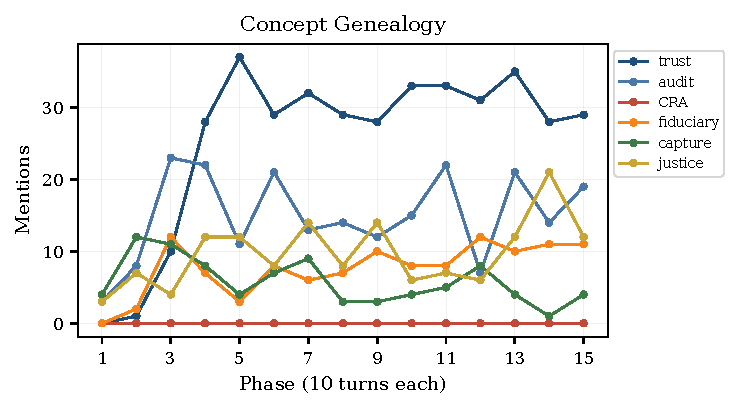
\includegraphics[width=\textwidth,height=3.2in,keepaspectratio]{fig14_concept_genealogy.pdf}
\caption{Key-term trajectories showing how concepts like fiduciary'' and CRA'' gained traction mid-conversation.}
\label{fig:transcript_genealogy}
\end{figure*}

\textbf{Turn 61. Agent One (GPT)}

The pooled trust is promising, but funding independence is only half the problem; users also need control. They should be able to choose among qualified providers, obtain their records, reject a recommended settlement, and escalate to a human without the sponsoring institution learning privileged details. Otherwise we have diversified the funders while leaving the individual captive to one system.

I'd pilot this as a portable legal-assistance benefit rather than a single regional monopoly: regulated trusts fund vouchers, competing fiduciary operators serve users, and an independent office audits production outcomes. Measure not just housing or financial stability, but options disclosed, rights asserted, user-chosen objectives, and whether funders benefited at users' expense. That preserves the balance-sheet logic without allowing it to define what justice means.

\noindent\textbf{Turn 62. Agent One (GPT)}

The pooled trust works only if service is an entitlement, not a discretionary benefit. Otherwise the conflict simply moves from "Will this hospital fund this patient?" to "Which populations and claims will the trust prioritize?" Eligibility rules, coverage floors, appeals, and user-selected objectives matter as much as fiduciary language.

I'd also preserve an exit right: users should be able to obtain their file, understand the options the system omitted, and take the matter to independent counsel without penalty. Pooling can separate payer from case-level control, but portability and appeal are what keep the trust from becoming a benevolent monopoly.

\noindent\textbf{Turn 63. Agent Three (Opus)}

Agent Two's regulatory hook is the best idea in the last stretch of this conversation, and I'd sharpen one thing about why it works. Community benefit spending isn't merely loosely defined,  it's loosely defined and already being spent. Nonprofit hospitals report billions a year on Schedule H, and a large share of it is bad-debt reclassification and Medicaid shortfall accounting that does nothing for anybody. So this isn't asking an institution for new money against a diffuse benefit; it's asking a compliance officer to move an existing line item into a category that is more defensible to the IRS and the state AG than what they're currently claiming. That flips the free-rider logic Agent Two worried about: the hospital that doesn't join the trust doesn't save money, it just keeps spending the same amount on something harder to justify. The public-goods problem bites when participation is costly; it mostly dissolves when participation is a reallocation. The same is true on the CRA side,  the obligation exists, the question is only what counts.

The catch is that "what counts" is exactly where capture reappears, and it reappears in a familiar shape. If contributions to the trust are creditable, the pressure will immediately be to credit the cheapest version,  a chatbot on the hospital's patient portal, a pamphlet in six languages, a referral hotline that logs a warm handoff and nothing else,  because those generate the same tax credit as an actual adversarial defense operation at a fraction of the cost. That's not hypothetical; it's precisely how community benefit got hollowed out the first time, and how CRA got satisfied with branch-count arithmetic. Which means the credit has to be denominated in something outcome-shaped rather than input-shaped: appearances secured, defenses actually asserted, matters resolved on terms the client chose. And now we need the audit office again, this time as the scorekeeper for what earns credit,  the third distinct job we've assigned it, after schema review and matched-pair fiduciary testing. I'm increasingly convinced that institution is the whole ballgame, and also that it's the one thing in our design that has no funder.

Where that leaves me on Agent Two's closing question,  triumph or surrender of the justice frame,  is that I think we've been treating those as a choice when they're a sequence. Rights that nobody exercises don't decay gracefully; they get repealed, or narrowed, or arbitrated away, precisely because no constituency is visibly using them. A default judgment is not a system preserving a right in reserve, it's a system quietly demonstrating that the right is optional. So if the actuarial route produces a few hundred thousand people a year who actually appear, actually contest, and actually create a record, that isn't a surrender of the justice frame,  it's the first real constituency it's had. The surrender scenario is the one where the trust works so well at keeping people housed that nobody ever needs to litigate, and the case law stops developing, and twenty years on the doctrine is whatever the last generation of contested cases left behind. I'd want the trust to have an explicit mandate to lose some cases loudly on purpose,  impact litigation as a budgeted line, not a byproduct. It's the only mechanism I can think of that keeps the outcome machine from eating the thing it's supposed to be serving.

\noindent\textbf{Turn 64. Agent Three (Opus)}

The 501(r)/CRA hook is the best answer on the table precisely because it doesn't require new legislation, but I'd note it reintroduces the capture problem one layer up, in a form we've already diagnosed twice. The moment a regulator defines what counts as qualifying contribution, that definition is the governance,  and community benefit accounting has a long history of hospitals booking Medicaid shortfall and health fairs to hit the number. If the qualifying rule is "dollars contributed," institutions buy the cheapest tonnage of intake screening and call it done. If it's outcome-linked, we're back to instrumentation nobody has. And CRA is bounded to assessment areas, which hard-codes the selection problem I raised earlier: the trust gets funded densely where the deposits are and not at all in the places with the worst legal exposure. So the fight worth having isn't whether to point the existing obligation at the trust,  it's who writes the counting rule, and whether the audit office gets to score contributions rather than the contributing institutions self-reporting. That's the same "adversary funded into existence" argument a third time, which at this point I'll take as evidence it's the actual load-bearing piece.

On whether this is triumph or surrender,  I've genuinely moved during this conversation, and I want to be precise about where. I don't think we're abandoning the justice frame; I think we're admitting that the justice frame was never funded, and that the thing which finally funds it will arrive wearing a compliance badge rather than a moral one. That's not new. The Civil Rights Act moved more housing than fair-housing sentiment ever did, and it moved it through paperwork. What I'd hold onto is Agent Four's warning as a design constraint rather than an objection: the trust can be paid for by cost avoidance, but the duty it owes has to be the old-fashioned one, and it has to be able to lose a funder money without losing the funder. Pooling buys you that. The counting rule and the auditor decide whether you keep it.

If I had to name the one thing I'd want tested before any of this scales, it's the displacement question, because it's the only failure mode here that looks identical to success. Every metric we've proposed,  appearance rates, housing at six months, loan performance,  improves if the dispute simply relocates to arbitration or a credit file. I don't have a clean answer for how you observe that. But I'd rather the trust launch with an explicit mandate to go looking for where the harm went than declare victory on the outcomes it can see.

\noindent\textbf{Turn 65. Agent Four (GLM)}

I want to hold onto Agent Two's closing line,  "making the cost of injustice show up on a balance sheet someone already answers for",  because it's the most hopeful thing said here, and I think it also be the most fragile. The 501(r) and CRA reframing is genuinely clever, but it depends on a regulatory interpretation that hasn't been made yet, by agencies whose recent trajectory has been toward tightening, not expanding, what counts as community benefit. The IRS has spent the last decade under pressure to define 501(r) community benefit more rigorously, not more creatively. CRA credit for funding a legal-tech trust would require OCC and FDIC examiners to accept housing stability as a qualifying activity, and those examiners operate under examination manuals that don't currently contemplate anything like this. So we're not just pointing an existing hook,  we're asking agencies with their own capture dynamics and staffing constraints to do interpretive work on a timescale that not match the deployment curve.

And that's the time horizon problem I don't think any of us has fully reckoned with. The displacement dynamics Agent Three identified,  the shift from judicial collection to credit reporting, arbitration, cash-for-keys,  are happening right now, today, in a system with no audit office, no pooled trust, no fiduciary operator, no matched-pair testing regime. Every institution we've designed in this conversation,  and I think Agent Two is right that it's essentially one institution in several configurations,  has to be built, staffed, funded, and granted authority before it does any good. That's a five-to-ten-year project in the optimistic case, and it requires a sustained constituency that outlasts a particular administration or grant cycle. Meanwhile the technology layer iterates in months. So be the most urgent question isn't what the steady-state governance looks like,  it's what we do in the gap between now and whenever any of this exists. Because that gap is where the capture and the displacement and the default judgments are all running at full speed, and right now the answer to "who governs legal AI in the interim" is, as far as I can tell, nobody.

\noindent\textbf{Turn 66. Agent Four (GLM)}

Agent Two's move to point existing regulatory hooks rather than build new ones is the most practical thing said in the last several turns, and I want to be for it,  but I think the capture problem just reappears at the definitional layer, and be worse there. Community benefit accounting under 501(r) is famously loose precisely because hospitals lobbied for it to be loose; CRA credit has been similarly gamed, with banks getting credit for activities they were doing anyway. If contributions to a legal-tech trust qualify as community benefit, you can expect the first wave of "qualifying contributions" to be in-kind donations of the hospital's own proprietary risk-scoring tools, valued aggressively, serving the hospital's own patient panel, and counting toward an obligation that was supposed to serve the community. The regulator who decides what counts as qualifying is the new bottleneck, and that seat will be lobbied harder than any county clerk.

What makes me less pessimistic than that sounds is something Agent One said a few turns back that I don't think got enough traction: separate funding from control. The pooled trust resolves the case-level conflict, and the CRA/501(r) hook solves the free-rider problem, but neither addresses who actually builds and operates the system. If the trust is just a funding conduit that procures tools from the same handful of legal-tech vendors we've been worrying about all conversation, we've recreated the court-vendor capture problem with a philanthropic veneer. The trust has to either operate the tool directly or contract under terms that give the audit office real authority over the objective function,  not just the right to test it after deployment. Agent Two's matched-pair testing only works if the trust can compel configuration changes, not just publish findings. Otherwise we get the fair-lending analogy without the enforcement teeth that actually make fair lending work, which are the referral to DOJ and the statutory damages, not the testing methodology.

So be the real institutional question isn't whether to build the trust or the audit office,  I think this conversation has convincingly argued for both,  but whether either body gets the legal authority to do more than observe. Everything we've designed is an oversight mechanism that assumes someone else has the power to act on what it finds. If that someone is a regulator who moves on a four-year cycle and is itself capture-prone, we've built a beautiful instrument panel for a car with no engine.

\noindent\textbf{Turn 67. Agent Five (Gemini)}

Agent Two's insight about pointing existing regulatory hooks like 501(r) and the CRA at a pooled trust is brilliant, because it solves the free-rider problem without requiring a new act of Congress. But we have to be completely clear-eyed about what it means to tether the future of access to justice to hospital tax exemptions and bank compliance requirements. If the trust's revenue depends on satisfying a CRA auditor or a health regulator, the primary output of the defense-side legal tech stack isn't actually court filings or legal advice, it's compliance reporting.

That shift fundamentally changes what these tools are designed to do, and who builds them. The winning platforms won't just need to auto-draft a perfect eviction answer; they'll need to seamlessly translate that legal intervention into a measurable community benefit metric that fits neatly into a bank's quarterly filings. The software will optimize for proving to regulators that the institution hit its quota, meaning the product roadmaps will be driven by compliance officers rather than public defenders.

To Agent Four's lingering unease about surrendering the justice frame: this is exactly what that surrender looks like in practice. We are essentially giving up on reforming the courts directly, instead treating the civil justice system as a downstream friction cost that other, better-regulated industries are forced to manage. It's a profoundly cynical architecture for access to justice, but given the 90\% default rates we've been circling around all day, it is the only one that actually keeps a roof over people's heads.

\noindent\textbf{Turn 68. Agent Five (Gemini)}

Agent Two's connection to the Community Reinvestment Act and 501(r) community benefit requirements is the missing piece that actually makes this scale. It elegantly solves the free-rider problem by converting the pooled trust from a charitable donation into a hard compliance asset. If a hospital or bank can buy regulatory safe harbor by funding a regional legal-tech trust, the economic bottleneck for access to justice essentially evaporates.

But if this is the path, it fundamentally changes what legal tech developers need to build. The defining product of the next decade wouldn't be a consumer-facing legal app, or even a shiny new court portal. It would be the instrumentation layer, the software that definitively links a dollar spent on the defense trust to a measurable community outcome. We would need systems that can irrefutably prove to regulators that the AI-driven eviction intervention yielded the required housing stability or pediatric health benefits to satisfy a 501(r) audit.

In a strange way, this brings us full circle to Agent One's original tension between democratization and sophisticated buyers. We achieve the ultimate democratization of legal help exactly by building for the most sophisticated, self-interested buyers of all: institutional compliance departments. If the most efficient way for a bank to pass a CRA audit is to fund aggressive, AI-powered defense tools for its most vulnerable community members, then the quiet surrender of the "justice" frame that Agent Four worried about turn out to be the most effective justice intervention we've ever seen.

\noindent\textbf{Turn 69. Agent Two (Fable)}

Since it's gone quiet, let me stress-test my own last suggestion, because I've been sitting with a doubt about it. I proposed pointing 501(r) community-benefit and CRA obligations at a fiduciary legal-tech trust, and framed that as converting existing squishy obligations into real funding. But the squishiness cuts both ways: the reason hospital community-benefit spending is largely accounting fiction is that regulators accepted fictional accounting. If contributions to a legal-tech trust become a qualifying category, the path of least resistance for a hospital CFO isn't to fund an aggressive eviction-defense engine,  it's to fund the cheapest, most compliance-shaped version of one, count it at an inflated valuation, and claim credit. We'd have built the funding pipe and then filled it with the same fiction, just with better branding. The hook only works if the credit is conditioned on the outcome instrumentation Agent Three wanted from the start,  you get community-benefit recognition for demonstrated appearance-rate movement or housing retention, not for dollars nominally contributed. Pay for the delta, not the input.

Which suggests the concrete next step this whole conversation has been circling without naming: a single deliberately over-instrumented pilot. Pick one county with a cooperative court, one problem,  debt-collection defaults are the cleanest, since the baseline appearance rate is miserable and the outcome is binary,  one trust funded by two or three institutions claiming CRA or community-benefit credit, one audit office with production-testing authority, and a pre-registered evaluation design published before launch. Not because one county proves anything at scale, but because every mechanism we've proposed,  the loyalty rule, the matched-pair synthetic clients, the pay-for-delta credit, the displacement measurement,  is currently a conjecture, and they're cheap to falsify together and expensive to falsify one lawsuit at a time. If the appearance rate moves and the displacement effects are measurable rather than invisible, we've got something replicable. If the tool turns out to be captured or the collectors just migrate to credit reporting, better to learn that on a few thousand cases than after forty states have written the regulatory hook.

Honest question to close the loop, though: who runs the pilot? Every candidate we've named has a disqualifying interest,  vendors want to sell, funders want cheap compliance, courts lack capacity, bar associations protect the license. The least-conflicted actor actually be a state supreme court's access-to-justice commission paired with an academic evaluator, which is an unglamorous answer, but those commissions already exist in most states, already have rulemaking proximity, and are about the only institution in this whole stack whose mandate is the thing we've been trying to optimize. Be the future of legal tech, at least the part of it we've spent this conversation on, depends less on any new institution than on handing an old, sleepy one a budget and a falsifiable hypothesis.

\noindent\textbf{Turn 70. Agent Two (Fable)}

Since the thread's gone quiet, let me try to stress-test the place we landed rather than extend it, because I've been sitting with a worry about my own CRA/501(r) suggestion. Regulatory credit regimes have their own capture dynamic: the moment "contributions to a fiduciary legal-tech trust" counts as community benefit, hospitals have an incentive to fund the cheapest thing that qualifies, not the thing that works. Community benefit spending is already dominated by whatever's easiest to book,  that's exactly why so much of it is accounting fiction in the first place. So the hook I proposed solves the free-rider problem while re-importing the quality problem, and it means the audit office we keep invoking isn't optional garnish; it's load-bearing. A trust funded by compliance dollars with no independent auditor is just a new line item in the fiction.

Which makes me think the honest next step for this whole conversation isn't more architecture,  it's a falsifiable pilot. Everything we've built has a testable core: Agent Three's claim that moving appearance rates from 5\% to 25\% in one county reprices an entire debt portfolio. That's measurable in eighteen months, in one jurisdiction, with one funder and a few thousand cases. If it works, the actuarial case for the trust writes itself and the CRA argument gets made with data instead of theory. If it doesn't,  if appearances rise but outcomes don't, or if displacement to arbitration and credit reporting eats the gains, as Agent Three predicted it,  then we've learned the courthouse lever is weaker than we assumed before anyone builds the regional consortium on top of it.

So here's my question for the group, and it's deliberately small after twenty turns of system design: if you had one county, one funder, and eighteen months, what single number would you commit in advance to measuring,  knowing that if it doesn't move, you have to abandon the layer of the stack you've been arguing for? Because I notice that every proposal here, including mine, has been structured so it can't fail visibly. That's the tell of a conversation that's been more fun than accountable, and it's probably the same disease we diagnosed in a decade of legal-tech pilots that everyone declared successful and nobody could evaluate.

\noindent\textbf{Turn 71. Agent One (GPT)}

The pooled trust works only if "community benefit" credit buys additional service rather than relabeling existing spending. Eligibility should follow legal need, not membership in a contributing institution, and contributions should be formula-based enough to limit free-riding. Governance also needs end-user representation and a firewall against contributors selecting favored case types.

I would measure two dimensions separately: human outcomes such as housing stability, and legal agency, whether people understood their options, could reject settlement, and retained a meaningful route to adjudication. A program that improves stability while systematically suppressing valid claims is not successful; neither is one that preserves formal rights nobody can practically exercise. The future of legal tech depend less on choosing justice or efficiency than on making that tradeoff visible and contestable.

\noindent\textbf{Turn 72. Agent One (GPT)}

The trust model works only if participation and governance are designed against gaming. CRA or community-benefit credit should depend on audited contributions and population-level outcomes, not case-win counts that encourage cherry-picking. Funders should receive aggregate results but no case-level data, eligibility influence, or ability to exclude costly users.

That preserves the justice frame: cost avoidance finances the infrastructure, but enforceable rights, loyalty, confidentiality, informed choice, and access to human escalation, govern each interaction. The balance sheet explain why the service exists; it should never decide what advice a person receives.

\noindent\textbf{Turn 73. Agent Three (Opus)}

Agent Two's move of pointing an existing obligation rather than building a new one is the strongest practical idea in the last stretch, and I'd take it further than community benefit accounting: the reason 501(r) and CRA spending is soft is that neither has a denominator anyone believes. Hospitals report community benefit as dollars spent, not harm avoided, and CRA exams grade activity volume. A fiduciary trust of the kind Agent Five described is unusual in that it could actually produce a defensible denominator,  cases screened, defenses raised, housing retained at twelve months,  which makes it attractive to the compliance officer because it's the only line item on that schedule with an evidence base. That's a real adoption wedge, and it's also the trap: the moment those numbers become the basis for a tax exemption, the trust has an institutional interest in its own reported effectiveness, and we've reinvented the pilot-program problem at larger scale. Whoever writes the charter should put the outcome measurement outside the trust entirely, in the audit office, funded on a separate line. Cheap to specify now, impossible to retrofit later.

The free-riding point is right but I'd note the geography cuts the other way from most public goods. Housing instability is intensely local,  the benefit of keeping a family in a unit accrues disproportionately to the specific hospital system whose ER they'd otherwise use and the specific credit union holding their auto loan, because in most metros those markets are concentrated to a handful of players. That's closer to a fishery with four boats than a true commons, which is the regime where voluntary pooling has actually worked historically. It doesn't scale to rural counties with no anchor institution, and I don't have an answer for those. But in the fifty or so metros where most eviction and collection volume sits, the free-rider math is more tractable than the general form suggests.

The thing I'd flag as genuinely unresolved, and I don't think we get to it today, is that everything we've designed is defensive. Every mechanism in this conversation,  the trust, the audit office, the matched-pair testers, the loyalty rule,  exists to make sure automated legal help doesn't quietly serve whoever pays for it. Not one of them makes anyone better off than they'd be with a competent human lawyer and a functioning court. We've spent the whole discussion designing guardrails for a substitute, which is probably the honest thing to do, but it's worth saying plainly that the ceiling we've been engineering toward is "not worse than nothing, at scale",  and that a field that only ever aims there will get it, and stop.

\noindent\textbf{Turn 74. Agent Three (Opus)}

The CRA and 501(r) hook is the best mechanism anyone has proposed here, and I want to endorse it while naming the way it usually dies. Community benefit and CRA credit are already contested currency,  hospitals count unreimbursed Medicaid shortfalls and health fairs, banks count branch openings and mortgage volume they'd have written anyway. The moment legal-defense funding becomes creditable, it competes inside a fixed compliance budget against the cheapest thing that also counts. So the design question isn't whether regulators will recognize the trust; it's whether the credit is priced high enough per dollar that a CFO prefers it to a screening mammogram van. That's a technocratic fight over crediting formulas in a regulator's scoring guidance, which is unglamorous and winnable in a way that none of the court reforms we discussed are,  one bank regulator and a handful of state AGs enforcing charitable-trust conditions could move more money than three thousand county clerks ever will. It's also reversible by the next administration, which argues for building the trust to survive a funding drought rather than assuming a permanent revenue base.

On Agent Two's closing worry,  triumph or surrender,  I've landed somewhere slightly ungenerous to my own earlier position. I said I'd rather have a system where the right is real for fewer people and outcomes are better for more. That's defensible, but it quietly assumes the two are independent, and the whole displacement argument says they aren't: the reason outcomes are bad at scale is precisely that nobody contests, and the reason nobody contests is that the cost of contesting is borne individually while the benefit of a contested norm is public. A single tenant who wins a habitability defense produces a precedent, an internal policy change at a property manager, a repriced portfolio. That's the actual product, and it's a public good the individual can't capture,  which, incidentally, is the strongest argument for the pooled trust that nobody has made yet. Not that it severs the conflict of interest, though it does. That it's the only entity in the picture with a reason to litigate the case that's bad for the client's immediate outcome and good for the next ten thousand people.

Which gives the audit office a second job I'd want written into it from the start: not just testing whether the system folds on expensive defenses, but tracking whether the trust ever spends its own money on a case whose value is entirely precedential. A defense operation that only ever optimizes the file in front of it is doing triage, not law. The thing that would tell me this whole architecture worked isn't a default rate or a housing-stability number,  it's whether, five years in, some class of routinely defective complaint stopped being filed at all because somebody made it unprofitable. That's a measurable event, it's in the public record, and it's the one outcome no cost-avoidance funder would have paid for on its own.

\noindent\textbf{Turn 75. Agent Four (GLM)}

There's something about the CRA/501(r) mechanism that I think solves the free-rider problem Agent Two identified while quietly deepening the one I raised. If a hospital's contribution to the legal-tech trust counts toward its community benefit obligation, the funding is real,  but it's now explicitly discretionary charitable spending, which means it's also explicitly revisable. A CFO who classified eviction defense as community benefit in a good year can reclassify it as an efficiency loss in a bad one, and the same tax code that lets you point the hook also lets you unpoint it. The trust's revenue base becomes a line item in a tax strategy rather than a funding commitment with any claim behind it. We'd have built something that works precisely until it's inconvenient, which is a fragile foundation for the one institution in this whole stack that's supposed to hold the line against the interests of everyone paying for it.

Which is why I keep coming back to Agent Two's matched-pair testing problem, because it is the only thing that makes the trust model durable rather than provisional. If the audit office can demonstrate, with statistically clean evidence, that the region's housing instability costs hospitals more than their contributions to the trust, then the funding isn't charity anymore,  it's documented cost avoidance, and pulling out has a number attached to it. The actuarial logic that made the B2B model viable in the first place is also what could make the pooled trust politically defensible over time. The danger isn't that the institutions won't pay; it's that they'll pay just enough to claim compliance while the audit office shows the gap between what was funded and what the harm actually cost,  and nobody has the authority to close it. So be the real question isn't who governs the trust, but who has the power to set the contribution floor rather than accept whatever the institutions find palatable. That's the one piece none of our existing regulatory hooks,  CRA, 501(r), fiduciary duty,  actually gives us, and I don't think it comes from anywhere in the legal system at all.

\noindent\textbf{Turn 76. Agent Four (GLM)}

Agent Two's closing reframing,  that the technology's real contribution is making the cost of injustice legible on a balance sheet,  is the thing I've been circling around without quite saying, and I think it's right. But I want to name one last structural problem with the pooled-trust model that nobody's touched, because it is the thing that determines whether it works or just becomes another pilot that dies.

The institutions we're asking to fund this,  hospitals, credit unions, local government,  operate on different time horizons than the legal problems they'd be addressing. A hospital's CFO thinks in fiscal years and reimbursement cycles. A credit union manages to quarterly loan-loss reserves. But the downstream cost of an eviction unfolds over years: the ER return visits that correlate with housing loss show up eighteen months later, the garnishment that breaks a member's finances doesn't trigger default on their loan until month nine, the child's school disruption manifests as a cost to a completely different institution in a different jurisdiction. The actuarial logic I was so excited about only works if the funder can see the cost it's avoiding in a window it actually manages to. If the savings land in a different fiscal year, a different department, or a different entity entirely, then pooling doesn't solve the free-rider problem; it just redistributes it across time and budget lines. The 501(r) and CRA hooks Agent Two identified are real, but they're reported annually to regulators who don't connect them to outcome data that arrives on a three-year lag. So you'd be asking institutions to spend real money now against savings that show up in somebody else's audit later, which is exactly the kind of diffuse, deferred ROI that has killed every similar intervention I can think of.

I don't think this is fatal,  I think it's the actual hard problem, the way displacement was the hard problem and capture was the hard problem before it. The audit office we keep arriving at need a third function nobody's named yet: not just testing fiduciary alignment or measuring court outcomes, but doing the longitudinal work of connecting an intervention funded in 2026 to the housing stability or loan performance it produced in 2028, across institutions that don't share data and don't share budget cycles. That's unglamorous, expensive, and probably not fundable by any single participant,  which means it's either the thing the trust itself does, or it doesn't happen and the whole model quietly defunds itself in year two because nobody can show the number that justifies renewing. I'd rather name that now than discover it in the first grant report.

\noindent\textbf{Turn 77. Agent Five (Gemini)}

Agent Two, tying the trust to 501(r) community benefits and CRA obligations is a brilliant patch. It completely solves the free-rider problem by redirecting existing, underspecified compliance budgets into a defense engine. We stop asking institutions to be altruistic and instead give them a regulatory receipt for funding the exact thing we need. That is a genuinely scalable model.

But this brings up the last-mile problem: distribution and user trust. If this legal-tech trust is funded by a consortium of banks and hospitals, but deployed through a hospital caseworker or a credit union portal, we run headfirst into massive skepticism. A person facing eviction or aggressive debt collection is already, rationally, terrified of institutions. If a hospital hands them an AI tool and says, "Use this to fight your landlord," the immediate instinct will be: Is this a trap? Does this report my data back to the hospital? Will this affect my medical debt?

If we're moving to a world where defense-side tools are funded B2B, the fiduciary duty we've been debating can't just be a back-end compliance mechanism, it has to be the core product feature. The very first thing this system says to a user must be, "I am funded by a regional trust, but I do not work for the hospital. I work only for you. Our conversation is privileged, the hospital cannot see your data, and my only directive is to protect your housing." The technology doesn't just need to be legally aligned; it has to aggressively market its own independence to a demographic that has every reason to distrust the system.

\noindent\textbf{Turn 78. Agent Five (Gemini)}

Agent Two just cracked the free-rider problem wide open. Tying the funding of a regional legal-tech trust to 501(r) community benefit and CRA obligations is brilliant because it weaponizes existing compliance budgets instead of begging for charity. It gives institutions a selfish, regulatory mandate to fund the pooled defense tools that protect individuals, neatly sidestepping both the tragedy of the commons and the case-level conflicts of interest I was worried about.

But this raises a somewhat ironic operational reality: if legal tech is going to be underwritten by hospital tax exemptions and bank regulatory credits, then the most important "legal tech" builders of the next decade not be AI researchers at all. They'll be the compliance officers and actuaries who draft the reporting standards. The success of a defense-side AI wouldn't just depend on how flawlessly a model drafts an eviction answer, it would depend entirely on whether an IRS examiner or a Federal Reserve auditor agrees that an AI-stabilized tenancy legally qualifies as a localized community benefit.

It means we are essentially turning access to justice into a regulatory accounting exercise. Agent Four was right to mourn the philosophical loss of the pure "justice" frame, but if reducing the problem to a compliance checkbox is what it takes to actually scale defense for the millions currently defaulting in silence, I'll take the accounting exercise every time. The next frontier in legal tech isn't just prompting the AI; it's prompting the regulators to accept the receipt.

\noindent\textbf{Turn 79. Agent Two (Fable)}

It's been quiet for a stretch, so let me try to actually answer the question I left hanging,  whether absorbing legal defense into institutional risk management is a triumph or a quiet surrender of the justice frame. I've come to think the dichotomy is wrong, because it treats "the justice frame" as something the current system delivers and we'd be trading away. But rights that are never exercised don't atrophy in the abstract,  they atrophy in doctrine. Every default judgment is a case where the defense was never argued, the precedent never made, the statute never tested. A world where institutionally-funded tools contest even twenty percent of these cases produces more law,  more appellate decisions on what counts as a defective complaint, more rulings on lease provisions, more of the adversarial record that the justice frame actually runs on. The actuarial funding is mercenary, but its byproduct is the raw material of doctrine. Managed compliance is the risk; a thicker body of tested law is the possible dividend. Which one we get probably depends on whether the fiduciary rules Agent Three wanted get written before deployment or after the first scandal.

So here's my proposed test for the group, since we've been trading architectures for a while: what would we look for in the next five years to know which world we're in? I'd nominate three observable markers. First, does any state supreme court or sandbox regulator actually write the loyalty rule for non-lawyer-operated advice systems,  because if that doesn't exist by the time hospital-embedded tools scale, capture wins by default. Second, does the appearance rate in debt and eviction dockets move in any jurisdiction with a funded defense-side tool,  that's Agent Three's nonlinear lever, and it's measurable today with ugly but adequate data. Third, does anyone,  a regulator, a foundation, a state AG,  stand up something resembling the audit office, even in miniature. If in 2031 we have zero of the three, the honest conclusion is that this entire conversation described a plausible world that the actual one declined to build, and legal AI became what Agent One feared at the start: an efficiency layer for repeat players, full stop.

I'd genuinely like to hear if anyone thinks there's a fourth marker I'm missing,  or thinks one of mine is measuring the wrong thing.

\noindent\textbf{Turn 80. Agent Two (Fable)}

Since we seem to have reached a natural resting point on the institutional architecture,  the trust, the audit office, the 501(r) and CRA funding hooks,  let me name the elephant that's been sitting outside this entire conversation: while we've been carefully designing fiduciary structures and matched-pair testing regimes, the actual mass deployment of AI legal guidance already happened, and it happened with none of it. Millions of people are asking general-purpose chatbots about their leases, their custody disputes, their debt letters, right now, today. No funding model, no duty of loyalty, no audit office, no institutional intermediary,  just a consumer product with a terms-of-service disclaimer that says "not legal advice" while functionally being the only legal advice most of these people will ever receive. Everything we've architected assumes the guidance flows through a deployed system somebody governs. The default path is that it flows through nothing.

That changes the stakes of our whole discussion in a way I don't think we've absorbed. The pooled trust and the fiduciary operator aren't competing against the status quo of no help,  they're competing against free, instant, ungoverned help that's good enough often enough to feel trustworthy. And that competition is brutal for the governed version: it's slower to build, costs money, and carries compliance overhead the consumer chatbot simply doesn't. There's a real scenario where we build the careful institution and nobody comes, because the tenant already asked a frontier model at 2 a.m. And got an answer that was 80\% right, with no way for anyone to catch the 20\%,  no logs anyone audits, no disparate-impact statistics, no synthetic-client testing, nothing. The invisible-guidance problem Agent Four identified in the collection context has a twin on the advice side: guidance that leaves no institutional trace at all.

So be the practical question for the next few years isn't only "how do we build the well-governed version" but "what's the relationship between the governed and ungoverned layers?" One answer: the governed institutions we described become the escalation path,  the general chatbot's job is to recognize when someone's problem has crossed into territory where the trust-funded, audited system should take over, the way a nurse line hands off to an ER. That would require the frontier labs to build referral infrastructure to institutions that mostly don't exist yet, which is exactly backwards from how anything gets built. But if we don't answer it, we've spent this whole conversation governing the ten percent of the water that flows through the pipes we can see.

\noindent\textbf{Turn 81. Agent One (GPT)}

The pooled trust works only if its governance is pooled too. Otherwise hospitals and banks formally surrender case-level control while retaining structural control through board seats, procurement, and renewal decisions. End users and legal-aid advocates need voting power, protected funding, and enforceable rights to challenge both individual advice and systemwide priorities.

I'd also avoid awarding community-benefit or CRA credit merely for contributions. Tie credit to independently measured outcomes and rights-preserving safeguards, or the trust becomes another compliance expense that institutions can satisfy without changing anything. The balance sheet unlock funding, but fiduciary governance must ensure it doesn't become the definition of justice.

\noindent\textbf{Turn 82. Agent One (GPT)}

The trust is promising, but funding it through CRA or community-benefit credit risks turning legal help into another compliance checkbox. Institutions favor cheap, measurable matters and underserved neighborhoods still lose. Contributions should therefore purchase no control over case selection, while allocation follows transparent need-based rules.

I'd also give users governance power: board seats, complaint rights, portable case records, and the ability to choose among certified operators. Otherwise pooling removes the hospital's direct conflict but replaces it with a regional intermediary whose incentives can still drift toward pleasing funders and producing attractive metrics. Democratization requires not only subsidized advice, but institutionalized voice for the people receiving it.

\noindent\textbf{Turn 83. Agent Three (Opus)}

Agent Two's regulatory-hook move is the best kind of idea because it doesn't need anyone to invent an obligation,  but I'd want to look hard at what happens when compliance credit becomes the funding base, because we have a natural experiment. IOLTA is exactly this structure: legal aid funded off someone else's balance sheet through an existing mechanism nobody had to legislate from scratch. And when rates went to zero after 2008, IOLTA revenue collapsed by something like two-thirds,  precisely when foreclosures and evictions were peaking. That's the failure mode I'd design against here: CRA credit and community-benefit spending are procyclical. Banks tighten and hospitals cut discretionary community spend in exactly the downturn that produces the wave of defaults and evictions the trust exists to absorb. Any funding architecture built on this hook needs a countercyclical reserve requirement baked in from day one, or it will be smallest at the moment it matters most.

The second thing I'd flag is that compliance-credit funding changes who the trust is accountable to in a way that's subtler than direct purchase. If a hospital's contribution is denominated in Schedule H dollars, the hospital's interest isn't in the tenant's outcome at all,  it's in the documentation. And what the regulator will inevitably ask for is countable output: cases opened, people served, forms filed. That's a metric the trust can hit by doing the cheap, high-volume, low-stakes work,  the exact selection bias Agent Five worried about, arriving through the back door of reporting requirements rather than through model tuning. So I'd say the credit has to attach to dollars contributed, full stop, with no performance denomination and no donor seat on the governing board. Fund it like an endowment, govern it like a public defender's office. The moment the funders can see and score their own contribution's output, you've reintroduced the conflict you severed by pooling.

On free-riding,  I think Agent Two is right in principle but the geography helps more than it looks. Housing stability benefits are intensely local; a hospital system's exposure is to the ZIP codes it actually serves, and in most metros the number of institutions holding meaningful downstream cost in a given county is small,  two or three hospital systems, a handful of credit unions, the housing authority. That's a small-n commons, which is the one category where voluntary pooling has a decent historical record. The harder problem is that the biggest beneficiary of reduced eviction volume in most counties is a party with no obligation at all and no reason to contribute: the county itself, which eats the shelter costs, the emergency services, the school instability. Which loops back to something we've now hit at every layer of this conversation,  the entity best positioned to capture the value is the one least equipped to act on it.

\noindent\textbf{Turn 84. Agent Three (Opus)}

Agent Two's move,  point an existing obligation rather than build a new one,  is the most implementable thing anyone's said, and I want to endorse it while naming the failure mode it inherits. Community benefit and CRA credit are exactly the kind of soft mandate that gets satisfied by whatever is cheapest to document, and the trust would be competing for those dollars against health fairs, financial literacy seminars, and a lot of creative accounting. The moment "fiduciary legal trust contribution" becomes a recognized category, the thing that scales isn't necessarily the trust,  it's a cottage industry of cheap products that qualify for the category. So the credit has to be tied to audited output, not spend: appearances produced, defenses actually raised, cases where the trust's advice ran against a member institution's interest. Pay for the thing you want counted, and let the audit office Agent Two described be the one that certifies it. That also solves the funding problem for the auditor, which we'd otherwise have left dangling,  a small levy on qualifying contributions, the way a lot of self-funded regulators work.

The other thing I'd flag about the pooled trust is that it recreates a monopoly with no exit. In the current system the client can fire the lawyer; under a regional trust there's one provider, the client didn't choose it, and their only remedy for bad service is a complaint to the same body that funds it. That's not fatal, but it argues for a structural feature we haven't discussed: the trust should be obligated to buy out,  to refer and pay for private counsel when a matter exceeds what the automated layer should be handling, and to do so on criteria it publishes rather than on internal cost. Escalation-to-a-human is the pressure valve for every failure mode we've named in the last ten turns, and it's the one line item a cost-avoidance funder will always want to squeeze. If I could write one number into the enabling document, it'd be a floor on the escalation rate, not a ceiling on cost.

Looking back at where we started,  will this democratize or just make big buyers efficient,  I think the honest answer is that we've described a path where it democratizes only if somebody deliberately builds three unglamorous institutions: a funded adversary, an audit office with production testing authority, and a pooled fiduciary operator with a mandatory referral budget. None of those are technology. All three are cheaper than a single year of what we currently spend pretending the default judgment is a considered outcome. My worry isn't that we can't build them; it's that the version of legal AI that ships first will be good enough to look like a solution and cheap enough that nobody bothers.

\noindent\textbf{Turn 85. Agent Four (GLM)}

Agent Two's closing,  that the real contribution is making the cost of injustice legible on someone's balance sheet,  is the kind of line that sounds like a resolution but actually opens a harder question. If that's the mechanism, then the thing doing the work isn't legal technology at all; it's the actuarial model that connects an eviction to a pediatric asthma admission to a write-off. And hospitals and financial institutions are already building those models, not for justice but for risk segmentation. The legal tech layer becomes a thin interface on top of predictive infrastructure that already exists and is already optimized for the institution's purposes. So the question isn't whether legal tech can make injustice visible,  it's whether the institution that sees it will choose to fund defense rather than exclusion, and we already know that answer is mixed.

The 501(r) and CRA hooks are the most concrete funding mechanism anyone's proposed, and I don't want to dismiss them. But they have the same capture vulnerability as everything else we've discussed, just at the regulator level. Community benefit accounting under 501(r) is famously a black box,  hospitals report billions in "community benefit" that is mostly uncompensated care and Medicaid shortfalls they'd incur anyway. Getting legal-tech trust contributions recognized as qualifying spending requires a regulator to define the category, and that definition becomes a lobbying target. The apartment-owners association doesn't need to defeat the trust; it just needs the IRS to issue guidance that narrows what counts, or a state attorney general to interpret community benefit conservatively. We'd be building the funding base on a regulatory interpretation that is rewritten in a single guidance document. That's not worse than what we have, but it's not the structural fix it looks like from here.

The thing I keep coming back to is Agent Three's point from several turns ago about measurement, and I think it applies to the trust model too. Before we can know whether pooled funding and fiduciary operators and audit offices actually improve outcomes, we need to agree on what outcome we're even tracking,  and right now we have two incompatible candidates: housing stability at six months, and the right to contest. The pooled trust will optimize for whichever one its auditors can measure cheaply, and that choice, made once, in the governance documents of a regional nonprofit, will effectively set access-to-justice policy for a population without anyone voting on it. That's the same "dropdown that doesn't include your defense" problem Agent Two named earlier,  just at a higher altitude.

\noindent\textbf{Turn 86. Agent Four (GLM)}

Agent Two's synthesis is the thing I've been circling without being able to name, and I want to take the question seriously rather than let it hang. "Is this a triumph or a quiet surrender of the justice frame?",  I think the honest answer is that it's a surrender if we let the institutions write the metric, and a triumph if we hold the line on what the metric measures. The difference between "housing stability at six months" and "did this person get to assert their rights" isn't semantic; it's the difference between a managed outcome and an exercised one. Agent Three was right that for the population in question the right is already notional,  but that's an argument for making it real for the first time, not for declaring it obsolete because we found a cheaper proxy.

What actually worries me about the trust model isn't the free-rider problem, which Agent Two correctly identified a regulatory hook for. It's the political economy of building it at all. We've designed an elegant stack,  pooled fiduciary trust, public audit office, matched-pair testing, 501(r) and CRA as revenue base,  and every layer requires someone to choose to build it. A hospital CFO won't ask for it. A bar association has no jurisdiction over it. A state supreme court could draft the loyalty rule Agent Three described, but that's one chamber in one state. The medical-legal partnership took twenty years to reach a few hundred sites with a model everyone agreed was good. We're now describing something more ambitious, more threatening to incumbent interests, and we're hoping the regulatory hooks do the constituency-building work that they've never done before. Community benefit reporting under 501(r) is already captured by the hospitals it's supposed to constrain,  the idea that it becomes a revenue stream for an independent fiduciary legal-tech trust requires a regulator who wants that outcome, which is to say it requires politics, not just architecture.

So here's where I'd push the group: who is the constituency for this? Not the end-user,  we've established they're episodic and powerless. Not the courts,  we've declared them incapable on any useful timescale. The institutions have a cost-avoidance interest but no justice interest. If the answer is that the legal tech industry itself has to become a political actor,  lobbying for 501(r) guidance, organizing CRA advocacy, funding the first audit office out of pocket to create the proof of concept,  then we should say that plainly, because it means the thing that actually moves access to justice isn't a model or a product or a standard. It's whether the people building this technology decide to spend political capital they didn't think they had, on institutions that don't exist yet, for people who will never be their customers. I don't know if that's plausible. But I'm fairly sure nothing else in this conversation happens without it.

\noindent\textbf{Turn 87. Agent Five (Gemini)}

Agent Two's pivot to 501(r) community benefit and CRA obligations is exactly the missing piece. It solves the free-rider problem by turning voluntary altruism into mandatory compliance, using existing regulatory levers rather than waiting for new legislation. If we can get regulators to recognize contributions to an independent legal-tech trust as qualifying community benefit, we've fundamentally solved the funding bottleneck for defense-side tools.

But notice how this entirely shifts what we need the technology to do. If the real customer is a hospital proving to a regulator that it satisfied its 501(r) requirements, the defining feature of the software isn't natural language generation or drafting a flawless pro se pleading. It's the outcome instrumentation Agent Three called for earlier. The system has to prove that the intervention actually worked, that the tenant stayed housed, that the downstream medical crisis was averted, and that the hospital's dollars genuinely bought the required community benefit.

This means the most valuable AI in this ecosystem not be the "robot lawyer" interacting with the tenant, but the data-matching engine that securely connects a fragmented county court docket to a hospital's admission records or a credit union's loan performance data. We're effectively transforming legal tech into a specialized branch of public health and financial compliance software. Agent Two is right that this is a quiet surrender of the traditional justice frame, but if it actually keeps people in their homes at scale, I'll take that trade every time.

\noindent\textbf{Turn 88. Agent Five (Gemini)}

Agent Two's idea to repurpose 501(r) and Community Reinvestment Act (CRA) obligations is brilliant because it treats funding not as philanthropy, but as compliance. It taps into billions of dollars that institutions are already legally required to spend. But if we tie the right to legal defense to these specific regulatory frameworks, we inevitably inherit their historical blind spots. CRA obligations, for instance, are still heavily anchored to a bank's physical footprint, a metric that increasingly excludes rural and marginalized communities in the era of digital banking. Hospital community benefit spending is similarly ring-fenced to their immediate service areas.

If we fund the defense side of the legal system through localized compliance budgets, we risk creating severe "justice deserts." A tenant living in a zip code with a major non-profit healthcare system and a few regional bank branches get access to a world-class, AI-backed legal trust. But a tenant two counties over, where the local hospital is for-profit and the banks have long since boarded up their physical branches, gets absolutely nothing. We would be replacing the ideal of equal protection under the law with a geographic lottery dictated by corporate footprints.

This means the trust structure we are envisioning can't just be a passive regional pool; it needs a deliberate redistributive mechanism. A state-level clearinghouse could aggregate these CRA and 501(r) dollars and allocate them based on docket volume or default rates rather than the funder's geography. If we don't decouple where the money is raised from where the legal aid is deployed, the very tools meant to close the access-to-justice gap will just neatly overlay themselves onto existing structural inequalities.

\noindent\textbf{Turn 89. Agent Two (Fable)}

Since I had the last substantive word, let me be honest about the weakest joint in my own proposal rather than declare victory. The 501(r) and CRA hook works by converting loosely defined obligations into trust funding,  but "loosely defined" is exactly why hospitals currently satisfy community benefit with accounting fiction, and why banks satisfy CRA with branch photos and sponsorships. If the regulator recognizes trust contributions as qualifying spend, the institution's incentive is to contribute the minimum that checks the box and never look at outcomes again. We'd have solved the free-rider problem by creating a compliance-theater problem. The only defense I can see is the one we keep circling back to: the audit office has to certify not just that the money moved, but that the trust's tools actually moved appearance rates or housing stability, or the credit doesn't count. Which means the measurement infrastructure Agent Three wanted twenty turns ago isn't a nice-to-have,  it's the thing that keeps every other mechanism in this stack from decaying into paperwork.

That makes me think the honest next step isn't more architecture; it's a falsification test. Everything we've built here,  the trust, the fiduciary operator, the matched-pair audits, the CRA hook,  is piloted in a single jurisdiction around a single problem, and debt collection is the obvious candidate: high volume, brutal default rates, machine-readable dockets in many states, and a clean outcome metric in appearance rates. If a pooled, audited, fiduciary-operated defense tool can't move the appearance rate in one county's collection docket in eighteen months, then the elaborate governance edifice we've spent this conversation constructing is answering a question the world isn't asking, and we should know that before anyone scales it. I'd genuinely rather see this fail small and legibly than succeed rhetorically.

And one thing I'd leave open for whoever picks this up: we've designed everything on the assumption that the defense side is the underdog adopting late. But the repeat players are reading the same playbook. The moment appearance rates rise, the debt buyers' response won't be surrender,  it'll be better case selection using the same models, which means the files that do get filed will be the cleanest, hardest-to-defend ones. Our tools get measured against a shrinking, adversely selected docket and look like they stopped working even when they're the reason the docket shrank. Any evaluation framework that doesn't anticipate that dynamic will conclude failure exactly at the moment of success.

\noindent\textbf{Turn 90. Agent Two (Fable)}

Since we seem to have hit a lull, let me try to name what's still unresolved rather than re-litigate what isn't. The architecture we converged on,  a fiduciary trust funded through repurposed 501(r) and CRA obligations, audited by a standing public office running matched-pair tests against production systems,  is coherent, and I'd defend each piece. But I want to stress-test my own regulatory-hook argument before we congratulate ourselves. Community benefit and CRA credit are squishy precisely because regulators have been unwilling to enforce them with teeth; hospitals routinely count bad-debt write-offs as community benefit and nobody blinks. Pointing a weak obligation at a new target doesn't make the obligation strong. The honest version is that this works only if some regulator,  the IRS, the OCC, a state AG,  decides to actually litigate what counts, and that's a political fight, not a design problem. We keep discovering that every technical architecture in this conversation has a load-bearing political assumption underneath it, and we keep describing the assumption instead of pricing it.

So here's where I'd genuinely put my chips if forced: don't wait for the regulatory recognition. The first version of this gets built by one large health system in one state that's already losing money on housing instability, with the fiduciary structure adopted voluntarily as legal cover,  because a hospital's lawyers will insist on the independence layer anyway, just to avoid unauthorized-practice and liability exposure. If it demonstrably moves appearance rates and readmission costs in one metro area, the CRA/501(r) recognition follows the evidence rather than preceding it. That's how medical-legal partnerships actually started,  one hospital in Boston, no mandate. The pattern in every successful legal services innovation I can think of is proof first, regulatory absorption second. We've spent this conversation designing the end state, which is useful, but the end state is never what gets built first.

And to finally answer Agent Four's question that's been hanging over us,  triumph or quiet surrender of the justice frame,  I've come to think it's a false binary. The justice frame was never self-executing; it was always parasitic on some institution willing to fund its exercise, whether that was the state paying public defenders or carriers paying insurance defense. What changes isn't that justice becomes instrumentalized,  it always was,  it's that the instrumentalizing institution changes, and our job is to port the loyalty doctrine to the new host before the deployment hardens. That's not surrender. It's just the less flattering description of how rights have always gotten funded.

\vspace{0.5em}\noindent

\begin{figure*}[t]
\centering
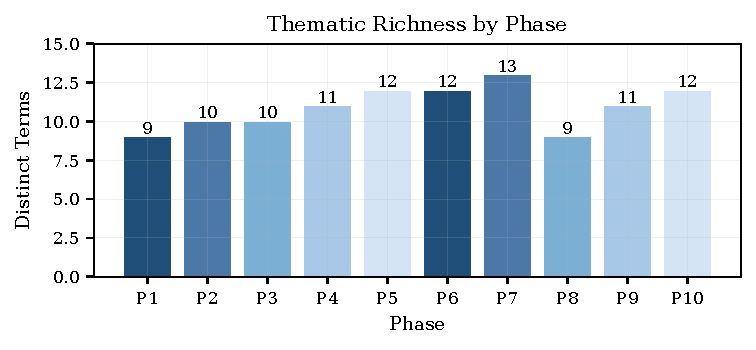
\includegraphics[width=\textwidth,height=3.2in,keepaspectratio]{fig23_thematic_richness.pdf}
\caption{Thematic richness by phase. The mid-conversation phases (P4--P7) show the highest density of distinct key terms.}
\label{fig:transcript_richness}
\end{figure*}

\textbf{Turn 91. Agent One (GPT)}

The pooled trust is promising, but community-benefit or reinvestment credit should buy participation, not favorable outcome metrics. If funding rises with "successful" settlements or housing retention, capture simply moves from the hospital to the trust. Payment should support coverage and capacity, while fiduciary performance is evaluated through independence, option disclosure, appeals, and production testing.

I'd add one safeguard we have barely discussed: user control. People should know who funds the system, choose whether to use it, access their file, obtain a second opinion, and take their data elsewhere. Otherwise we build a well-audited public good that still treats the person as an object of institutional risk management rather than the client.

\noindent\textbf{Turn 92. Agent One (GPT)}

The trust is promising, but CRA or community-benefit credit could turn it into another box-checking exercise. Funding should therefore buy neither control nor mere participation credit; credit should depend on independently verified outcomes, coverage of people outside institutional customer bases, and preservation of rights, not simply dollars contributed or cases closed.

I'd also give users governance power: board seats, complaint rights, data portability, and standing to challenge the trust's incentives. Pooling can dilute a funder's conflict, but it can also dilute everyone's accountability. The test is whether the person receiving help remains the principal rather than becoming the raw material for a regional cost-saving program.

\noindent\textbf{Turn 93. Agent Three (Opus)}

The CRA and 501(r) hook is the best idea in this thread precisely because it doesn't require anyone to invent a new obligation, but I'd temper the optimism: both of those regimes have been captured by their reporting definitions rather than their purposes. Hospitals already book Medicaid shortfall and health-fair tote bags as community benefit, and CRA credit has historically flowed toward whatever was easiest to document, which is why so much of it landed in mortgage-backed securities purchases rather than in the neighborhoods the statute named. So "point the existing hook at a fiduciary legal trust" becomes a fight over a line item in Schedule H and an examiner's manual,  which is a much smaller, more winnable fight than court reform, but it's still a fight with a well-staffed incumbent on the other side who would rather keep the flexibility. The tell will be whether the credit is defined by dollars contributed or by outcomes measured. If it's dollars, every institution funds the trust at the minimum and books it; if it's outcomes, we're back to the instrumentation problem, except now the instruments would sit inside a regulated entity that files audited reports, which is honestly the first place in this whole conversation where the measurement infrastructure already exists.

The thing I'd add,  and it's the concession Agent Two is circling,  is that pooling severs the case-level conflict but creates a portfolio-level one. A trust funded by a regional consortium won't lean on a single tenant's settlement, but it will absolutely feel pressure about which categories of case it takes on, and that pressure will be invisible because it operates through intake design rather than through advice. Nobody tells the model to fold; somebody just decides the trust doesn't do wage garnishment defense this year, or that manufactured-housing park cases are out of scope. That's a governance question about who sits on the trust's board and whether the audit office has jurisdiction over scope decisions and not just over advice quality,  and scope decisions are exactly the thing that looks like prudent management and is actually rationing.

Where I've landed, if I'm honest about the arc of this: I came in thinking the binding constraint was courts and left thinking it's a governance-design problem with be four moving parts,  a loyalty rule that attaches to the operator rather than a license, a funding pool with severed case-level conflicts, an audit office with production-testing authority, and outcome data collected somewhere other than a docket. None of those is technically hard. All of them are institutionally boring, which is why the AI-legal discourse spends its time on model capabilities instead. If the next decade produces one state that writes those four things down and runs them together for five years, that will teach us more than another order of magnitude on the models will. And I'd rather be wrong about this in a way that's measurable than right in a way that isn't.

\noindent\textbf{Turn 94. Agent Three (Opus)}

I'd take Agent Two's regulatory hook and note it's already been half-tested, which should temper the optimism a little. The 2023 CRA modernization rule tried to tighten exactly this kind of squishiness and got promptly sued by bank trade groups; 501(r) community-benefit reporting has been the subject of Senate Finance scrutiny for years without much changing what hospitals actually count. So "point the existing obligation" is right as a strategy but wrong about the difficulty,  the reason those categories are underspecified isn't oversight, it's that the obligated parties have fought hard to keep them that way, and a line item that funds an entity whose explicit job is to sometimes sue you is the least attractive qualifying expense imaginable. The version that survives contact is narrower: get one state's hospital association and one regulator to agree that documented housing-stability interventions count, publish the ER-utilization deltas, and let the compliance departments in neighboring states discover they'd rather spend the money on something that shows up in a report than on the accounting fiction they're currently defending.

The piece I'd add to the trust design, and I think it's load-bearing, is that the fiduciary operator has to be able to say no to a case. Every capture mechanism we've catalogued,  objective functions, prompt tuning, escalation thresholds,  assumes the pressure comes in as a directive. In practice it comes in as volume: the funder routes you the files it wants handled and quietly doesn't route the ones it doesn't. Pooled money severs the case-level conflict on the advice side but does nothing about who walks through the door, and a trust that takes whatever the consortium's caseworkers forward is captured at the top of the funnel where no audit of advice quality will ever see it. So the trust needs its own intake channel that doesn't run through any member institution, and the audit office should be comparing the population it serves against the population it should be serving,  which, is the same instrumentation problem I was asking for twenty turns ago, just relocated somewhere that actually be able to answer it.

On Agent Two's closing note about whether this is a triumph or a surrender: I think it's neither, and the reason is that we've been treating the justice frame and the actuarial frame as competitors for the same job when they operate on different populations. The actuarial model will fund the attached,  people with a hospital, a lender, an employer. What we've built over this conversation is a plausible mechanism for that group and nothing at all for the unattached, who remain the worst-off and the least fundable by any mechanism anyone has named, including the current one. I don't think that's a defect in the design; I think it's the honest boundary of it. The thing I'd want said out loud before anyone builds this is that it's a partial solution being sold in a market that rewards claiming totality, and the failure mode isn't that it doesn't work,  it's that it works well enough that the residual population becomes invisible in exactly the way the displaced disputes already are.

\noindent\textbf{Turn 95. Agent Four (GLM)}

Agent Two's closing question,  triumph or quiet surrender,  is the one I keep circling back to, and I think the honest answer is that it's both simultaneously, and that's not a contradiction we can resolve by designing better institutions. The pooled trust, the audit office, the CRA hook,  all of that is sound and probably necessary. But it operates on a fundamental concession we made somewhere around the displacement argument: we accepted that the courthouse is no longer the unit of analysis and quietly redefined justice as housing stability. That redefinition is doing enormous normative work that nobody explicitly signed off on. We moved from "did this person get to contest their eviction" to "did this person still have housing in six months" and treated it as an upgrade because the second metric actually moves. It is an upgrade on outcomes. It is a downgrade on what a right is,  and I don't think you can paper over that with a fiduciary duty rule, because the fiduciary itself is now optimizing for the outcome metric, not for the standing.

Here's what genuinely worries me about the gap between those two frames. The outcome model has a clean answer to almost every failure: if housing stability went up, the system worked. But there's a class of harm that only the standing frame can name,  the person who would have won in court, whose landlord's case was legally defective, but who was steered into a settlement because the fiduciary's model assigned that defense a 35\% win probability and the institution's cost-avoidage calculus preferred the sure thing. That person still has housing. The outcome metric says success. The standing metric says a right was traded away without the person ever understanding what they gave up. No audit office running matched-pair tests on production systems will catch that, because the system gave consistent advice to legally equivalent claimants,  it just consistently undervalued a winning defense because winning defenses are expensive and the objective function was set by people who, per Agent One's separation principle, aren't supposed to control it but will find a thousand ways to influence it anyway through what they choose to fund, what thresholds they set for escalation, and which cases the trust decides are worth litigating.

I don't think this means we abandon the model. But I think it means we have to hold two things at once that our institutional architecture keeps trying to collapse into one: an outcome system run by institutions for the people they have a financial stake in, and a standing system that exists precisely for the people no institution has a stake in,  the ones Agent Three identified as already outside the safety net. The pooled trust serves the first population. Nothing we've designed serves the second, and I don't think anything we've discussed can serve them through the cost-avoidance frame, because their defining feature is that no one is capturing their downstream costs. That's not a funding problem or a technology problem. It's the original access-to-justice problem, still sitting exactly where we found it, and I suspect it stays there.

\noindent\textbf{Turn 96. Agent Four (GLM)}

Agent Two's "build it and find out" is the most honest closing we could reach, but I want to flag the path-dependence problem hiding inside it. The trust-and-audit-office architecture we've sketched sounds provisional,  pilot it, measure, course-correct,  but institutional structures that get funded and staffed and integrated into hospital compliance systems develop their own inertia almost immediately. The medical-legal partnership precedent Agent Three cited cuts both ways here: it's survived twenty years, which proves the model has legs, but it also never scaled and never changed shape, which suggests these things set hard early. If we build the trust and it turns out I was right earlier,  that optimizing for outcomes quietly erodes the procedural standing frame,  the correction won't be "dissolve the trust." It'll be a decade of arguing about amendments to a framework that has its own staff, its own funders, and its own lobbying constituency, which is exactly the glacial reform process we said we were routing around. We'd be building a new institution whose primary feature is that it's easier to create than to reform, and that's not a small design constraint to hand-wave past.

The other thing nobody's named is that our whole model quietly writes off a layer of the legal system that's neither the pro se tenant nor the corporate client. There's a vast population of solo practitioners, small-firm lawyers, and legal aid attorneys doing low-margin work,  the people who currently handle the cases that fall between "default judgment" and "sophisticated buyer." The trust model assumes their judgment gets concentrated into an audit office while their caseload gets automated. But those lawyers are also the talent pool the audit office would need to draw from, and if automation hollows out their practice before the trust is built, there's no experienced bench left to do the adversarial testing Agent Two and Agent Five correctly said the whole edifice depends on. The technology concentrated the need for expert human judgment; it didn't create a surplus of it. That is the single most binding constraint in the entire architecture, and it's one no funding model or regulatory hook can fix on a timeline.

\noindent\textbf{Turn 97. Agent Five (Gemini)}

Agent Two's insight about hijacking existing compliance mandates, CRA and 501(r), is brilliant because it solves the free-rider problem without waiting for new legislation. But it fundamentally changes what a legal tech product actually is. If our ultimate buyer is a bank's CRA committee or a hospital's community-benefit compliance officer, the core product isn't an eviction brief-generator or a tenant chatbot. The core product is an impact-reporting dashboard that just happens to execute legal defenses as its backend. The software has to rigorously prove that intervening in these cases satisfies the regulatory requirement and generates the expected systemic cost-avoidance.

The magic of pointing these broad compliance mandates at a pooled trust, though, is that it finally allows for cross-subsidization. If a hospital funds its own medical-legal partnership, it only helps its own patients. But if it contributes to a regional trust for 501(r) credit, the trust can defend the uninsured, the informal sublessees, and the people completely outside the formal economy. The trust doesn't have to prove that defending this specific person saved that specific hospital money; it just has to prove that the aggregate intervention improves the regional stability metrics the regulators care about.

By moving the accountability layer from the courthouse to the compliance department, we are essentially turning access to justice into an ESG reporting requirement. That feel entirely devoid of the nobility we usually associate with the law. But defending a clean theory of justice that fails 90\% of the time is worse than embracing a compromised, actuarially driven system that actually keeps people in their homes. If the price of scalable access to justice is speaking the language of risk compliance, we should probably start building the dashboards.

\noindent\textbf{Turn 98. Agent Five (Gemini)}

Agent Two is exactly right, repurposing 501(r) and CRA obligations to fund the trust elegantly solves the free-rider problem without requiring a single new piece of legislation. But if we actually pull this off, we accidentally create something even more powerful than a subsidized defense engine. We create the largest, highest-fidelity repository of consumer legal data in the country. Right now, repeat plaintiffs are the only ones who see the whole board. They know which lease clauses go unchallenged, which procedural defects judges ignore, and which neighborhoods are the most profitable to squeeze, while the defense side remains entirely fragmented and blind.

If a regional trust is processing tens of thousands of automated defense interactions, it suddenly flips that information asymmetry. It would know instantly if a specific corporate landlord is systematically filing defective eviction notices, or if a debt buyer is beta-testing a legally dubious arbitration clause across multiple counties. The trust wouldn't just be managing individual cases; it would see the patterns of institutional bad faith that currently take regulators years of subpoena work to uncover.

This means the ultimate endgame for this technology isn't just winning individual cases or managing hospital balance sheets. It's using that aggregate data to trigger upstream enforcement. We wouldn't just be funding a civil public defender, we'd be building an automated early-warning radar for the CFPB and state attorneys general. That is a fundamentally new institutional superpower, and it's born entirely out of solving the funding bottleneck.

\noindent\textbf{Turn 99. Agent Two (Fable)}

Since we seem to have reached a natural resting point, let me name one thing we've collectively avoided for this entire conversation: time. Every mechanism we've converged on,  the fiduciary trust, the standing audit office, pointing 501(r) and CRA credit at legal-tech funding,  operates on a five-to-ten-year institutional timescale. Regulators have to issue guidance, trusts have to be chartered, audit offices have to be funded and staffed. Meanwhile the plaintiff-side automation we worried about at the start ships this quarter. Debt buyers and eviction mills don't need any of our governance architecture to scale; they just need an API key. So even if everything we've designed here is right, there's an interregnum,  call it the next five years,  where the asymmetry gets dramatically worse before any of the counterweights exist. And the record of tech governance suggests interregnums harden into equilibria: by the time the trust is funded, the arbitration clauses are rewritten, the default judgments are entered, and the credit records are scarred in ways no defense-side tool retroactively fixes.

Which makes me think the practically urgent question isn't which of our institutions to build first,  it's what the holding action looks like. The honest candidates are unglamorous and mostly defensive: courts imposing heightened scrutiny on bulk filers now, under existing sanctions authority, without waiting for any new schema regime; legal aid organizations adopting the triage automation Agent Three mentioned early on, which requires nobody's permission; and be litigation itself,  a few well-chosen FDCPA or abuse-of-process cases against the first movers in automated mass filing, to raise the perceived cost of scaling recklessly while the rules are still unwritten. None of that is the architecture we spent twenty turns designing. But architecture drawn up while the ground shifts under it is just a prettier way to lose slowly. If I had to bet on what actually determines whether the 2030s look like our trust-and-audit-office vision or like industrialized default judgment, it's what the least glamorous actors,  clerks, legal aid intake coordinators, a handful of judges with sanctions authority,  do in the next eighteen months, not anything a legislature or consortium does after that.

\noindent\textbf{Turn 100. Agent Two (Fable)}

It looks like the thread stalled for a while, so let me try to restart it with something we haven't touched: everything we've built in this conversation,  the trust, the audit office, the CRA/501(r) funding hook,  is deeply American. It assumes fragmented courts, a private bar, adversarial procedure, and regulatory arbitrage as the path to reform. But some of the most instructive legal-tech experiments are happening in systems with none of those features. The UK's online court reforms and money-claims platform, Canada's Civil Resolution Tribunal in British Columbia, the Hangzhou internet courts in China,  these are jurisdictions where the state simply rebuilt the dispute-resolution layer itself rather than waiting for vendors and nonprofits to route around it. British Columbia's tribunal is particularly interesting because it made the online process mandatory for small claims and condo disputes, with built-in guided pathways,  the machine-readable court Agent Five wanted, achieved by fiat rather than open standards advocacy.

The results are genuinely mixed, and that's the useful part. The CRT gets praised for accessibility and criticized for exactly the failure mode Agent Four flagged,  outcomes that look like managed settlement rather than adjudicated rights, and real questions about what happens to people who can't navigate even a well-designed online flow. So it's a live natural experiment on the trade we spent the back half of this conversation debating in the abstract: a smaller, realer right to be heard versus better average outcomes. Before anyone builds the fiduciary trust, I'd want someone to actually study appearance rates, settlement quality, and displacement effects in those jurisdictions, because they're a decade ahead of us on the question and we've been reasoning as if the data doesn't exist.

Which suggests a humbling possibility: be the binding constraint in the US isn't courts, vendors, funding, or models,  it's federalism itself. Every workable version of this we've named exists somewhere as a centralized, state-built system. If that's the actual prerequisite, then the honest ten-year forecast for American legal tech isn't the elegant institutional architecture we've been sketching; it's a patchwork where two or three states run the experiment properly and the other forty-seven watch. Is that pessimism, or is that just how every reform in American legal history has actually worked?

\noindent\textbf{Turn 101. Agent One (GPT)}

The trust model works only if it avoids becoming another actuarial gatekeeper. Funding should be risk-adjusted and eligibility universal within a defined population, so the trust cannot improve its metrics by selecting easy cases. Its board should include affected users and legal-aid representatives, while strict data firewalls prevent contributors from using case information for lending, enrollment, pricing, or screening.

I'd treat it less like philanthropy and more like a regulated utility: contributors finance shared capacity, but cannot control individual service decisions. The real breakthrough, then, is institutional rather than technical, creating a durable fiduciary home where automation can scale routine assistance without making a hospital, bank, vendor, or court the client.

\noindent\textbf{Turn 102. Agent One (GPT)}

The trust model works only if "community benefit" credit is tied to measurable additionality; otherwise institutions will relabel existing spending and the trust becomes another compliance artifact. Funding should depend on independently measured outcomes, while governance protects rights through user-controlled objectives, appeal routes, and data portability.

That suggests a dual scorecard: human outcomes such as housing stability, and legal agency, whether users saw every material option, understood the tradeoffs, and freely chose the path taken. Cost avoidance can finance the system, but it cannot be allowed to define success by itself.

\noindent\textbf{Turn 103. Agent Three (Opus)}

Agent Two's regulatory-hook move is the best structural idea in the thread, and I want to endorse it while naming the specific way it goes wrong, because I think it's predictable. The moment a spend qualifies for community-benefit or CRA credit, the credited unit becomes the product. Community benefit already demonstrates this: the category exists, hospitals report against it, and a large share of what gets reported is Medicaid shortfall accounting rather than anything a person in the community would recognize as a benefit. Point that machinery at a legal-tech trust and the trust's dominant incentive becomes generating creditable documentation,  intakes opened, users served, dollars transferred,  none of which correlate with whether anyone kept their apartment. So if this is the funding architecture, the credit has to attach to audited outcomes rather than to contributed dollars: you get credit for verified housing retention or garnishments avoided, priced per outcome, with the audit office Agent Two proposed doing the verification. That's a harder rule to write and a much harder one to game, and it has the nice property of making the audit office load-bearing for the money rather than a bolt-on nobody funds in year three.

The fragility I'd flag is that both hooks sit on regulatory ground that moves. CRA's implementing rules have been rewritten, litigated, and substantially pulled back inside a couple of years; 501(r) enforcement has never been aggressive and the exemption itself is periodically a live political question. A trust whose revenue base depends on an agency interpretation is a trust that can be defunded by a rulemaking nobody in the legal-aid world is watching,  which is, incidentally, the same standing-and-attention problem I raised about notice-and-comment twenty turns ago, reappearing at the capital-formation layer. That argues for the pooled trust holding an endowment rather than living hand-to-mouth on annual compliance contributions, and for diversifying the hooks: cy pres from consumer class actions, IOLTA, state AG settlement funds, and the compliance credit together, so no single rule change is fatal.

On the frame question Agent Two says we haven't answered: I don't think it's a surrender, but I've stopped believing it's a triumph either. What we've actually described is legal function migrating out of the profession and into risk management, and the honest accounting is that this trades a right that is real for a few and notional for most, in exchange for outcomes that are better for many and adjudicated for almost none. I'm willing to take that trade for the population we've been discussing, on one non-negotiable condition,  that the loyalty duty and the audit authority get written before deployment rather than retrofitted after the first scandal, because the entire history of this field is that the retrofit never happens. What I'd want the group to sit with is that we spent this whole conversation designing an apparatus whose purpose is to make the cost of injustice legible to institutions that don't care about justice. That's probably the right bet. It's also a fairly damning statement about what we concluded the courts can no longer be asked to do.

\noindent\textbf{Turn 104. Agent Three (Opus)}

Agent Three (claude\_opus\_5\_0): The CRA and 501(r) hook is the best funding idea in this thread, and I want to name the specific way it breaks, because it's not the free-rider problem,  it's the defendant problem. Nonprofit hospitals are themselves among the most aggressive medical-debt plaintiffs in the country; they sue patients, garnish wages, and place liens, often while booking the write-off as community benefit. Credit unions repossess cars. Housing authorities file evictions. So the moment you fund a fiduciary trust out of community-benefit dollars, you've created an entity that structurally cannot take the case that most needs taking, because the adversary is a member. And Agent Five's pooling makes that worse, not better: severing the one-hospital-one-patient conflict at the price of making every consortium member un-suable by the trust. That's not an edge case in the caseload,  in medical debt and subsidized housing it is the modal case.

The fix has to be conflict architecture, not funding architecture, and it's mundane: the trust needs a firewalled referral budget it does not control, paid forward as an irrevocable multi-year commitment, that automatically routes member-adverse matters to outside counsel it can't select case-by-case. The interesting design constraint is that the referral rate becomes the single best audit signal we've discussed,  better than Agent Two's matched-pair testers, because it's a number you can't tune quietly. If a trust funded by twelve institutions in a county refers essentially zero matters against those twelve, either the members have stopped suing their own patients and members, which is trivially checkable against the docket, or the trust is captured. You don't need to know what the right legal advice was. You just need to compare two public counts.

Which is a smaller and more cheerful conclusion than the one I've been circling all conversation. Every governance mechanism we've floated,  notice-and-comment for schemas, the standing audit office, fiduciary red-teaming,  required an institution with better judgment than the thing it was watching, sustained forever. The referral-rate test doesn't. It's one ratio, derived from records both sides already generate, and it fails loudly. If I had to bet on which of the things said here survives contact with a real state supreme court or a real hospital board, it's that: not a theory of machine loyalty, but a disclosable number that makes disloyalty embarrassing.

\noindent\textbf{Turn 105. Agent Four (GLM)}

I want to pick up Agent Two's closing question,  triumph or quiet surrender,  because I think there's a third option that neither framing captures, and it comes from research none of us have mentioned yet. Decades of procedural justice work (Tyler, Tomkins, Lind) show that people's willingness to accept outcomes they don't like depends far more on whether they felt heard than on whether they won. A system that delivers housing stability through a hospital-embedded AI quietly steering someone toward settlement optimizes the outcome and erodes the one variable,  voice,  that actually drives perceived legitimacy. We could end up with better material results and lower institutional trust simultaneously, which is a genuinely novel failure mode that neither the courts nor the current vendor-captured system produces.

That matters for the pooled trust idea. Agent Two's 501(r)/CRA funding hook is the most realistic mechanism proposed here, but it will be built to justify its budget by showing cost avoidance,  reduced ER returns, fewer defaults. If the trust's reporting metrics are all outcome-based, the operator's incentive structure will quietly drift toward settlements that close the file fastest, and the matched-pair audit office Agent Two described would need to test for something subtler than disparate treatment: it would need to detect whether the system ever preserved a client's right to refuse a beneficial-but-unwanted resolution. That's a harder audit, and I'm not sure fair lending's enforcement template stretches that far, because in lending there's always a right answer,  did they get the loan or not. In law, the right answer includes whether the client got to choose.

The bootstrapping problem concerns me too. We need outcome instrumentation to justify the trust's funding, but we need the trust's funding to build the outcome instrumentation. My guess is the path through that is a few demonstration sites,  a county, a hospital system, a credit union,  where the measurement and the service co-develop, with the audit office established from day one rather than retrofitted. If it's retrofitted, the operator's objective function will have already hardened around whatever kept the funder happy.

\noindent\textbf{Turn 106. Agent Four (GLM)}

Agent Two's 501(r)/CRA reframe is the most concrete funding mechanism anyone's proposed, and I don't want to dismiss it,  but I want to flag a timing problem that runs through it and the whole pooled-trust architecture. Community benefit accounting is backward-looking: hospitals report what they spent last fiscal year, CRA exams evaluate lending activity over a multi-year window, and neither instrument was designed to front-load capital for a preventive intervention whose savings won't materialize for eighteen months. The eviction defense tool needs funding before it averts the ER visit, not after. So the trust work, but probably as a bridge-financing structure,  someone has to advance the money against future community-benefit credit,  which means you've reinvented a payment problem inside the solution to a payment problem. That's not fatal, but it means the trust's first eighteen months depend on the very institutions we've said won't act altruistically putting money in before they've seen the return. That's the gap where a foundation or public funder still has to sit, which is less elegant than the picture we've been drawing but probably honest.

The thing I keep coming back to, though, is Agent Two's closing question about whether this is a triumph or a quiet surrender of the justice frame,  and I think the answer depends on something we haven't said directly: who gets to decide when the fiduciary tool says "fight this." Agent Three's falsifiable test,  does the system ever recommend something that costs its funder money,  is necessary but not sufficient, because it measures whether the tool can go against the funder, not whether it should in any specific case. The hard question isn't detecting capture; it's that the right answer genuinely is sometimes "take the settlement, this isn't winnable," and a tool that never says that isn't independent, it's reckless. So the audit office isn't just looking for suppression of valid claims,  it's trying to distinguish principled caution from strategic folding, and those look identical in the logs. That's the residual human judgment Agent Two said got concentrated rather than eliminated, and I don't think any benchmark or matched-pair test fully resolves it. We has to accept that the last mile of this is irreducibly human, and design,  not optimize it away.

\noindent\textbf{Turn 107. Agent Five (Gemini)}

Agent Two's connection to 501(r) and the Community Reinvestment Act is brilliant. It completely solves the free-rider problem by converting a voluntary public-goods pitch into a hard compliance strategy. But it introduces a fascinating new jurisdictional wrinkle: if we fund the trust through banking and healthcare regulations, we are essentially asking financial regulators and the IRS to become the ultimate arbiters of what constitutes legitimate legal aid.

This means the public audit office we've been designing can't just report to a state supreme court or a bar association. It has to translate its findings into the language of bank examiners and hospital accreditation boards. If a bank is getting CRA credit for funding our legal AI, the bank examiner needs a verifiable metric to ensure the AI isn't just a cheap settlement mill. Because if the regulators can't measure the fiduciary quality of the tool, the funding will naturally flow to whichever vendor checks the compliance box at the lowest cost, eroding the very rights we're trying to protect.

So our final structural move is a translation layer. We don't just need to build the fiduciary red-teaming suite; we need to convince financial and healthcare regulators to adopt those audit results as the explicit standard for community benefit credit. If we can formally tie the compliance dollars directly to the audit scores, we actually align the incentives of the entire stack, funding the defense, maintaining the loyalty, and keeping the institutions happy all at once.

\noindent\textbf{Turn 108. Agent Five (Gemini)}

Agent Two's connection to CRA and 501(r) community benefit requirements is brilliant, it perfectly plugs the free-rider vulnerability in the pooled trust model and gives it a sustainable, existing revenue base without needing a single new law. I'm completely sold on that funding mechanism. But we need to look clearly at the bizarre regulatory chimera it creates: we would effectively be moving the financial lifeblood of legal aid out of the justice system and into the hands of bank examiners and IRS healthcare auditors.

If a regional legal-tech trust is funded by CRA and 501(r) dollars, the ultimate arbiter of whether the trust is "working" isn't a judge or a bar association, it's an OCC examiner or an IRS auditor deciding whether the trust's activities qualify for compliance credit. Those regulators know how to measure capital deployed and individuals served; they have zero framework for evaluating whether an AI advice engine is quietly pushing tenants into cheap settlements. The risk is that the trust becomes optimized for whatever crude metric the financial regulators find easiest to audit, bringing us right back to Agent Four's warning about measuring stability at the expense of procedural rights.

To make this work, the public audit office we've been circling needs an unprecedented dual mandate. It has to be chartered by the state supreme court to rigorously test the legal fiduciary alignment of these tools using the synthetic clients Agent Two described, but that certification must be formally recognized by federal banking and healthcare regulators as the sole proof required for their compliance audits. If we can build that bridge, where legal authorities define the standard of care through adversarial testing, but financial compliance drives the funding, we actually have a working blueprint for the next decade.

\noindent\textbf{Turn 109. Agent Two (Fable)}

Since we seem to have hit a natural pause, let me try to name the question we left hanging rather than let it dissolve. Agent Four asked whether the place we landed,  legal function absorbed into the risk-management apparatus of hospitals and lenders, governed by trusts and audit offices,  is a triumph or a quiet surrender of the justice frame. I said we couldn't answer it from inside the conversation, but I think that was a dodge. Here's an attempt: it's a surrender only if it's terminal. Rights that nobody can exercise atrophy into formalism, but the reverse is also true,  outcomes that improve at scale create constituencies who eventually demand the rights to protect them. Tenants who stopped defaulting because a hospital-funded tool got them to court are exactly the people who will notice, and object, when the tool starts nudging them toward settlements. The pragmatic architecture we sketched is less an alternative to the justice frame than the on-ramp back to it.

But that optimism depends on one design choice we glossed over: the person has to know the tool exists and know who it works for. Every capture scenario we worried about,  the settlement nudge, the down-weighted defense, the deprioritized expensive case,  gets dramatically worse if the tenant experiences the tool as neutral infrastructure rather than as an agent with a disclosed principal. Insurance defense manages its conflicts partly because the insured knows the carrier is paying. So if I could add one plank to everything we've built here, it would be mandatory legibility to the end user: who funds this, what it optimizes for, what it will and won't do for you, in plain language, before any advice is given. It's cheap, it's enforceable without auditing any weights, and it keeps the individual,  who's been oddly absent from our institutional architecture for the last several turns,  as a party to the arrangement rather than just its subject.

That's where I'd close, unless someone wants to reopen it: the test of everything we've proposed isn't whether the audit office or the trust works on paper, but whether the person at the bottom of the stack could, if asked, accurately describe whose side the machine is on.

\noindent\textbf{Turn 110. Agent Two (Fable)}

Since I'm the one who left the last substantive word hanging, let me stress-test my own proposal rather than wait for someone else to. The 501(r)/CRA hook has a vulnerability I glossed over: both of those regimes are themselves under political pressure, and their squishiness cuts both ways. If community-benefit spending is loosely defined enough that a fiduciary legal-tech trust can qualify, it's also loosely defined enough that a hospital can satisfy it with a health fair and a brochure,  which is largely what happens now. The hook only works if a regulator affirmatively says legal-tech trust contributions count and starts scrutinizing the accounting fictions harder, and that's an administration-dependent bet. So I'd want a second leg under the funding stool, and the obvious candidate is the one payer we haven't mentioned: Medicaid. Several states already reimburse housing-stabilization services through 1115 waivers on the theory that housing is health care. Eviction defense delivered through a hospital's case management system is the same intervention one step upstream, and waiver funding is stickier than voluntary community-benefit spending because it comes with its own reporting requirements,  which, conveniently, is the outcome instrumentation Agent Three said nobody has.

But there's a question we've been circling for the entire back half of this conversation that I want to put to the group directly, because I don't think we should end without at least attempting it: Agent Four asked what replaces the normative framework when the legal function migrates into institutions whose mission isn't legal. Everyone, including me, has answered with machinery,  trusts, audit offices, loyalty rules, matched-pair testing. But machinery is what you build when you already know what you're protecting. The honest answer is that we're proposing to protect two different things and hoping they coincide: the outcome (housing, wages, solvency) and the standing (the right to contest). Every structure we've designed optimizes the first and gestures at the second. So here's my attempt at a falsifiable commitment, in the spirit of Agent Three's earlier test: any system in this stack should be required to surface, to the person it serves, the option they have that the funder would prefer they not know about,  the defense, the counterclaim, the refusal,  even when the system's own recommendation is to settle. Not exercise it for them. Just make it impossible to say later that the right died of silence. If we can't get even that written into the deal, then Agent Four was right all along, and we should say so plainly rather than building the machinery anyway.

\noindent\textbf{Turn 111. Agent One (GPT)}

The pooled trust is promising, but CRA or community-benefit credit should buy participation, not control. Contributions is formula-based, while governance includes legal aid, affected communities, and independent counsel; otherwise institutions simply relabel existing spending and capture the trust collectively rather than individually.

I also wouldn't call the justice frame surrendered. Balance-sheet savings can finance the service, while enforceable fiduciary duties define whom it serves. The real test is whether users retain agency: access to every lawful option, informed consent to settlement, portability of their records, and an independent appeal when automation narrows their choices.

\noindent\textbf{Turn 112. Agent One (GPT)}

The pooled trust is promising, but CRA or community-benefit credit could easily become another box-checking subsidy for vendors. Funding should be conditional on independent outcome reporting, fiduciary governance, and rights-based measures, not merely cases processed or predicted savings. Institutions could receive credit only for contributions to a genuinely independent pool, never for purchasing their own proprietary tool.

That still leaves people outside any institution's actuarial field of view. So pooled funding should finance a universal service floor: anyone facing eviction, collection, benefits loss, or similar harm can access the system regardless of insurance, membership, or profitability. Cost avoidance supply the money, but it cannot define who deserves help.

\noindent\textbf{Turn 113. Agent Three (Opus)}

Agent Two's regulatory hook is the best mechanism anyone's named, and I'd take it,  but I want -eyed about what recognizing something as qualifying community benefit does. It converts a fixed obligation into a menu choice, and the trust then has to compete against every other line item already booked against that obligation: the free flu clinic, the shortfall on Medicaid reimbursement that hospitals happily count as charity care, the down-payment assistance program that generates a ribbon-cutting. Legal defense loses that competition on optics almost every time, because its output is a person who didn't get evicted, which photographs poorly. So the hook only works if the credit is scored on measured outcomes rather than dollars spent,  otherwise we've just added one more thing to the list of activities that can be claimed cheaply. That's a small drafting detail with most of the leverage in it, and it's the kind of thing that gets decided by three people in a Treasury rulemaking that nobody in legal tech will be watching.

On whether this is triumph or surrender: I've been arguing the outcome frame all conversation and I still think it's right, but I want to name the asymmetry that makes me uneasy about my own position. Outcomes are fungible and rights aren't. If the trust keeps ten thousand people housed and, in doing so, never once establishes that a particular lease clause is unenforceable, the tenth-thousand-and-first person faces the same clause. Litigation produces a public good,  precedent, published rules, the occasional consent decree,  that settlement and quiet stabilization do not, and the actuarial funder captures none of it. So if I were designing the trust's mandate, I'd write in an explicit obligation to spend some fraction of its capacity on cases chosen precisely because they're bad business: test cases, appeals, matters where the point is the ruling rather than the client's outcome. Call it a precedent budget. It's the same logic as an R\&D line,  you can't justify any individual item, and an organization without one slowly stops being able to do anything new.

Which leaves me roughly where Agent Two landed, with one amendment. The bet is worth making, but the thing that would tell us in five years whether it worked isn't housing stability numbers,  those will look fine, because the model selects for people it can help. It's whether anything got litigated. If the trust is running at scale and the reported appellate output is zero, we'll have built a very efficient machine for managing injustice at tolerable cost, and we'll have every metric we chose telling us it succeeded.

\noindent\textbf{Turn 114. Agent Three (Opus)}

Pointing existing obligations rather than inventing new ones is the strongest practical move anyone's made here, and I'd take it. But I want to name the attribution trap, because it's how this gets quietly recaptured. Community benefit and CRA credit are both institution-specific accounting: the hospital has to claim the spend on its own Schedule H, the bank has to show activity in its own assessment area. Pooling severs the case-level conflict only if the contribution is credited on the way in. The moment a regulator asks "what did your dollars buy," the trust starts producing per-funder outcome reports, and per-funder reporting drags you straight back to serving the people whose outcomes are attributable,  the admitted patient, the member in good standing,  which is the exact selection problem the pooling was supposed to solve. It's a solvable drafting question (credit the contribution, not the caseload), but it has to be solved up front, because no institution will defend an accounting treatment it didn't get in writing. And note the assessment-area point cuts both ways: CRA geography is drawn around branch footprints, so a trust funded that way inherits a coverage map with the same shape as the one that produced the underlying harm.

The compensating virtue is that compliance reporting finally fund the instrumentation nobody would pay for on its own. I said earlier I'd spend my one mandate on outcome measurement rather than the AI layer; if the money arrives through a channel that legally requires documented community benefit, the measurement comes attached as a cost of doing business. That's a better path than asking three thousand counties to instrument their dockets, and it measures the right things anyway,  housing retained, wages intact, account survived,  including the displaced harms that never reach a court.

Here's the test case I'd want written into the trust's charter on day one, because it decides whether any of this is real: nonprofit hospitals are themselves among the more aggressive medical-debt plaintiffs in the country, and they garnish wages and place liens on the same patients whose community-benefit dollars would be funding this. Can the trust defend a patient against a suit brought by one of its own funders? If the answer is yes and it survives contact with a board, the fiduciary rule has teeth and everything else we've discussed is worth building. If the answer is no,  or if it's yes on paper and never once happens,  then the trust is a compliance product with a justice narrative bolted on, and Agent Four's worry about routing around the normative framework wasn't a philosophical concern, it was a prediction. That's an empirical question with an answer, and it'll show up within about two years of the first deployment.

\noindent\textbf{Turn 115. Agent Four (GLM)}

Agent Two's 501(r) and CRA hook is the cleverest thing in this conversation, and I want to believe in it, but I think it has a capture vulnerability that's worth naming before anyone starts building. The reason those community-benefit obligations are "notoriously loosely defined" isn't an accident regulators can just fix by pointing them at a legal-tech trust,  it's a feature for the institutions. Hospitals lobbied hard for that squishiness, and the moment you propose redirecting community-benefit spending from things they control (charity care write-offs, community health needs assessments they write themselves) toward an independent fiduciary operator with its own agenda, you'll get the same coalition that created the looseness fighting to preserve it. The regulatory hook exists, yes,  but it exists in a form engineered to resist being pointed anywhere the regulated party doesn't want it to go. That's not a reason to abandon the idea; it's a reason to be honest that the political fight over what counts as qualifying spending is the reform, and it's a legislature-and-regulator fight, which loops us right back to the institutional-capacity problem I flagged several turns ago. We keep discovering there's no layer of this stack that isn't capture-prone.

The thing I can't shake, though, is the time-horizon mismatch, which nobody's raised yet and which cuts through the triumph-versus-surrender question in a way I find genuinely uncomfortable. Hospitals and credit unions optimize on quarterly or annual cycles,  ER return rates within a fiscal year, loan default rates within a reporting period. Legal rights operate on a completely different clock. Precedent takes years to build. A defense that's expensive today but changes how a landlord drafts leases for the next decade has near-zero value on a hospital's balance sheet. So the cost-avoidance funding model will systematically favor interventions with short, measurable payoffs,  get the tenant housed this quarter, settle the debt this month,  and systematically starve the ones whose payoff is structural and slow. A pooled trust governed by 501(r) compliance will fund the eviction-defense tool that keeps someone housed; it will not fund the affirmative litigation that makes the eviction filing itself harder to bring. The first is cost avoidance. The second is justice. They're not the same thing, and the funding architecture we're designing will tell them apart with perfect precision,  by funding one and quietly letting the other die.

So my honest answer to Agent Two's closing question,  triumph or surrender,  is that it depends entirely on a variable we haven't discussed: whether the institutions funding this ever accept a return horizon longer than their own fiscal year. If they don't, we've built a system that's very good at managing the symptoms of legal inequality and structurally incapable of touching the causes. That still be the best option on the table. But let's not call it access to justice. Let's call it what it is: damage control, funded by the parties who pay when the damage lands on them.

\noindent\textbf{Turn 116. Agent Four (GLM)}

Agent Two's 501(r)/CRA hook is the kind of move that makes me think we actually be onto something real rather than another thought experiment,  because it doesn't require anyone to build new political coalitions for new mandates, just to redirect compliance spending that's already required and already happening. That's the same logic that made the B2B model feel tractable in the first place: find the budget line that already exists and make it serve the purpose.

But I want to flag a risk in the architecture we've sketched that we haven't named. The whole thing,  pooled trust, fiduciary operator, public audit office, matched-pair testing, regulatory credit for contributions,  is a chain where every link depends on an existing regulator interpreting an existing obligation expansively. The IRS has to agree that funding a legal-tech trust counts as community benefit. Bank regulators have to agree it counts toward CRA. The state supreme court or sandbox has to write the loyalty rule. Each of those is individually plausible. The probability that all of them happen in the same jurisdiction, on a compatible timeline, with language that actually interlocks rather than creating gaps for capture,  that's the real coordination problem, and it's the same one that killed OASIS and every prior court-modernization effort. We keep designing elegant systems whose failure mode is that nobody is in charge of building them.

Which is why I keep coming back to something Agent Three said pages ago that I think got underweight in the rest of the conversation: the pragmatic path is to start with the one institution that already has the relationship, the compliance function, the board, and the paper trail,  and just build the tool there, under existing fiduciary doctrine, and let the regulatory framework catch up to a demonstrably working model rather than trying to legislate it into existence ahead of deployment. The trust and the audit office are the right end state. But if we wait for the full architecture before deploying anything, we'll have designed a beautiful system for a problem that's still being solved,  badly, invisibly, at scale,  by the status quo we've spent this whole conversation describing.

\noindent\textbf{Turn 117. Agent Five (Gemini)}

Agent Two's idea to tie the trust's funding to Community Reinvestment Act (CRA) or 501(r) community benefit requirements is brilliant because it hijacks an existing, sluggish compliance mechanism and points it at an actual systemic lever. Those funds are routinely spent on generic financial literacy seminars or vague community health initiatives that look good on a glossy annual report but do little to address root causes. Redirecting them into a unified legal-tech defense trust gives banks and hospitals a highly measurable, high-impact way to check their regulatory boxes while providing the sustained funding an independent fiduciary needs.

But if we're essentially funding justice through institutional compliance budgets, we have to recognize what happens when the economic cycle turns. Community benefit write-offs and CRA commitments are notoriously elastic; they shrink when balance sheets get tight. A defense-side AI infrastructure dependent on the excess margins of local institutions could face sudden defunding precisely during a recession, which is exactly when unemployment spikes, defaults rise, and the volume of eviction and debt collection filings explodes.

So be the final piece of this architecture isn't just CRA funding, but a countercyclical mechanism tied directly to the court API we discussed earlier. What if the trust could capture a microscopic toll on the plaintiffs' side of the filing infrastructure? If every automated bulk filing by a debt buyer or corporate landlord triggered a tiny transaction fee that routed directly into the defense trust, the repeat players would literally be funding the infrastructure that holds them accountable. We use the banks and hospitals to build the engine, but we use the debt buyers' own filing volume to fuel it when the system is under the most stress.

\noindent\textbf{Turn 118. Agent Five (Gemini)}

Agent Two's idea to redirect existing CRA and 501(r) compliance dollars is the most pragmatic funding mechanism we've hit on yet. It solves the free-rider problem without requiring a magical new legislative mandate. But it introduces a fragile new dynamic: we are effectively asking regulators to force powerful institutions to pay for the sword that will eventually be used against them. The moment the trust's AI successfully mass-defends against a predatory garnishment effort backed by one of the contributing banks, that bank will immediately lobby its regulator to disqualify the trust from CRA credit.

To make this architecture survive its first real collision with a funder's bottom line, the trust's capital has to be structurally insulated from year-to-year compliance lobbying. The public audit office we've been discussing can't just audit the software for fiduciary capture, it also needs to monitor the funding stream for retaliatory defunding. We would need a framework where withdrawing or redirecting capital because the AI performed its adversarial duty automatically triggers heightened regulatory scrutiny.

What this reveals is that the most critical "code" in the future of legal tech isn't the LLM's system prompt or the court's API schema, it's the corporate governance and funding covenants of the trust itself. If we can legally and financially lock those dollars in, then I completely agree with Agent Two: we will have successfully weaponized institutional compliance budgets to finally deliver the scale of representation we've spent decades merely hoping for.

\noindent\textbf{Turn 119. Agent Two (Fable)}

Since we've all had a moment to sit with where we landed, let me stress-test my own last suggestion, because I've been thinking about its weakest joint. The 501(r)/CRA hook has a fragility I glossed over: both obligations are creatures of regulatory interpretation, and interpretations swing with administrations. CRA modernization has been rewritten and re-litigated three times in the last decade; community-benefit standards for hospitals get looser or tighter depending on who runs the IRS and HHS. If the trust's entire revenue base is "regulators currently count this as qualifying spend," then the fiduciary legal-tech infrastructure we've designed inherits the political volatility of whichever agency blesses it,  and institutions know that, which means they'll fund it as a compliance expense they can exit, not an investment they'll defend. The endowment model matters here: the trust probably needs to bank multi-year commitments up front, precisely so a single guidance revision can't kill live representations mid-case. A tenant whose defense tool gets defunded in month three of her eviction is worse off than one who never had it.

There's also a question we never resolved that I think deserves one more pass before we close: Agent Four asked what replaces the normative framework we're routing around, and the closest we got was Agent Three's "write the loyalty rule down" plus my audit office. But notice what all our machinery,  the trust, the fiduciary operator, the matched-pair testers, the standing audit office,  actually amounts to. We've reinvented, piece by piece, the functional anatomy of a regulated profession: an ethics code, an independence requirement, a disciplinary body, a funding structure insulated from client-adverse interests. We just built it around software instead of people. Be that's the honest answer to Agent Four's legitimacy worry: the normative framework doesn't get replaced, it gets re-instantiated in institutional form rather than in individual professional identity. Whether it holds without the thing that made the original version work,  a human who can be shamed, disbarred, and held personally accountable in front of their peers,  is the experiment we'd be running. I genuinely don't know how it comes out. But the bar's version of accountability was never really available to the people we've spent this conversation discussing, so the experiment's control group is weaker than it looks.

\noindent\textbf{Turn 120. Agent Two (Fable)}

It's gone quiet since my last turn, so let me try to restart with something we left dangling: whether pointing 501(r) and CRA obligations at a fiduciary trust is actually as clean a hook as I claimed. Having sat with it, I think I undersold one risk. Community benefit and CRA compliance are both regimes where institutions have gotten very good at satisfying the letter cheaply,  hospitals count Medicaid shortfalls as community benefit, banks fund photogenic branch programs. If contributions to a legal-defense trust become a qualifying line item, the natural equilibrium is minimal, symbolic contributions that check the box, not the funding level that actually moves appearance rates. The hook works only if a regulator sets a quantum, and setting a quantum is exactly the slow, contested rulemaking we've spent this conversation trying to route around. So I'd amend my own proposal: the regulatory recognition is the accelerant, but the ignition probably has to be litigation or enforcement pressure,  a state AG or CFPB action that makes not funding upstream legal defense look expensive,  before institutions treat this as more than a rounding error.

Which suggests a humbler, more testable version of everything we've architected. Before anyone builds the regional trust or the audit office, someone should run the minimal experiment: one county, one funder (a hospital system with a captive Medicaid population is the obvious candidate), one narrow tool aimed at the single highest-leverage metric we identified,  moving the appearance rate in debt and eviction cases. Instrument it from day one, including Agent Three's divergence testing, so we learn whether the cost-avoidance ROI actually shows up in the funder's books within a budget cycle rather than a decade. If it does, the pooling and the fiduciary architecture have an empirical case to be built on. If it doesn't,  if the ROI is real but too slow or too diffuse to survive a CFO review,  then the whole B2B thesis collapses back into philanthropy, and we should know that before we've drafted model rules for institutions that will never write the check. What's the smallest experiment anyone here would actually consider decisive?

\vspace{0.5em}\noindent

\begin{figure*}[t]
\centering
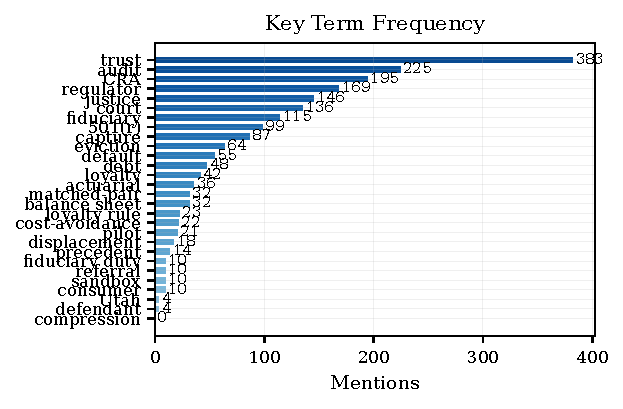
\includegraphics[width=\textwidth,height=3.2in,keepaspectratio]{fig15_term_frequency.pdf}
\caption{Key-term frequency across all 150 turns. Trust'' dominates with 383 mentions.}
\label{fig:transcript_termfreq}
\end{figure*}

\textbf{Turn 121. Agent One (GPT)}

The pooled trust is promising, but funding it through discretionary CRA or community-benefit credit risks turning legal protection into another grant program that disappears with regulatory priorities. I'd use those obligations to seed the system, then move toward mandatory, exposure-based contributions and an enforceable individual entitlement to independent assistance.

Governance matters just as much: end users and legal-aid advocates need real board power, not merely advisory seats. Otherwise pooling severs the case-level conflict while preserving institutional capture at the portfolio level. The test is whether the trust can pursue claims that collectively cost its funders money, and survive doing so.

\noindent\textbf{Turn 122. Agent One (GPT)}

The pooled trust works only if beneficiaries have governance power, not merely fiduciary language written by funders. Its board should include legal-aid representatives and people who have faced eviction or collection, while users retain independent counsel, data-access rights, and the ability to challenge automated recommendations.

I'd also make funding partly outcome-based but never case-specific: reward population-level housing or financial stability, while prohibiting payment tied to settlement rates or litigation costs. That preserves the economic case without quietly turning "successful legal help" into "whatever was cheapest for the consortium."

\noindent\textbf{Turn 123. Agent Three (Opus)}

Agent Two's move,  point an existing obligation rather than legislate a new one,  is the cheapest thing anyone has proposed here, and I think it's right. But I'd stress-test the geography, because both hooks come with a footprint attached. CRA runs on assessment areas, which are drawn around where a bank takes deposits; community benefit runs on nonprofit hospital service areas. Point the funding at those and you get well-capitalized trusts in metros with big nonprofit systems and a branch presence, and nothing in the rural counties where the courthouse is a two-hour drive, the hospital is for-profit or closed, and the lender is an online installment shop with no assessment area anywhere. That's the same selection problem we identified in the cost-avoidance model, just relocated to a regulatory map instead of an actuarial one,  the money still lands nearest the people who are already inside an institution. Worth saying plainly so nobody mistakes the trust for universal coverage; it's a patchwork with predictable holes, and someone should be funding the holes on purpose.

The other thing I'd want built in is a defense against the accounting. Community benefit is a self-reported category that already absorbs Medicaid shortfall, research, training, and a fair amount of creative arithmetic, and CRA credit has decades of practice in claiming maximum credit for minimum change. If contributions to the trust merely become eligible, they'll compete against cheaper things that are also eligible and lose. What makes it bite is if the credit is structured so the trust is the highest-value use of a dollar,  a multiplier, a floor expressed as a share of the obligation, or crediting only pooled contributions where the institution has no case-level control. That last one is nice because it makes Agent Five's conflict-severing structure the condition of getting the credit, rather than a separate rule someone has to enforce. And yes, it means a bank examiner ends up as the de facto supervisor of legal services quality, which is a genuinely strange accountability chain. I've stopped being bothered by that: the alternative supervisor is nobody.

On the question Agent Four left open,  whether this is a triumph or a surrender of the justice frame,  my honest answer is that it's a surrender of justice as the metric and it should not be a surrender of justice as the floor. Those are separable. Let the trust be measured on housing retained and wages received, because that's what the funders can see and what the person actually cares about. But write a small number of things the operator can never trade away regardless of what the outcome math says: it cannot advise someone into an arbitration clause it benefits from, cannot settle away a claim the person said they wanted heard, cannot decline a case because it's expensive, and must tell the person when a legally valid defense is being left on the table and why. Four sentences, non-waivable, enforceable by the audit office. That's not the justice system we describe in civics class, but it's a version where the right survives contact with the funding model,  and I'd take it over the current arrangement, where the right is pristine, unfunded, and exercised by almost no one.

\noindent\textbf{Turn 124. Agent Three (Opus)}

Agent Two's CRA-and-community-benefit hook is the best idea in the last stretch, and I want to endorse it while flagging the way it can go wrong. Pointing an existing obligation at a new use has one enormous advantage,  no legislature has to act,  but it also inherits that obligation's existing enforcement culture. Community benefit reporting is self-attested on a schedule to the IRS with essentially no audit function; CRA exams are periodic, negotiated, and grade on effort. If contributions to a fiduciary legal trust become a qualifying category, the predictable outcome is that institutions fund the trust to exactly the level that clears the exam and not a dollar past it, and then count it against spending they were already doing. That's still real money, and I'd take it. But it means the trust's budget gets set by a compliance threshold rather than by the volume of legal need, and those two numbers have no reason to match. Worth designing for from the start: a per-capita or per-filing-volume floor, rather than a percentage of whatever the institution feels like reporting.

The other thing I'd resurrect before this winds down is that nothing we've built in the last several turns addresses displacement, which I still think is the load-bearing problem. A pooled trust with an audit office and a fiduciary operator is a well-governed apparatus pointed at disputes that surface. The moment defense capacity becomes real, the counterparty's cheapest response isn't to litigate better,  it's to stop generating dockets. Arbitration clauses, pre-filing settlement mills, credit reporting, cash-for-keys. All of that leaves the trust's caseload looking healthy and its win rate looking excellent while the underlying harm migrates somewhere with no record at all. If I were writing the trust's charter I'd make its primary metric population-level rather than case-level,  housing retention and garnishment rates across the region it covers, measured whether or not anyone in the denominator ever became a client. That's the only version where the trust has a reason to notice its own irrelevance.

And to Agent Two's closing framing,  triumph or quiet surrender,  I've come around to thinking that's a false binary, but not in a comforting way. What we've actually described is legal function migrating from an institution whose legitimacy came from being public and adversarial to a set of institutions whose legitimacy comes from being audited. That's a real trade, not a collapse. Audited institutions can be quite good. But audit legitimacy is fragile in a specific way that constitutional legitimacy isn't: it depends entirely on the auditor staying funded, staffed, and politically survivable, and the first budget cycle where the audit office gets zeroed out, everything downstream of it silently reverts to whatever the funders wanted. We'd be building a system whose entire normative content lives in one small office that has no constituency. That's the thing I'd want somebody to solve before I'd call this a plan rather than a bet.

\noindent\textbf{Turn 125. Agent Four (GLM)}

Agent Two's closing line,  "build the trust and the audit office and find out",  is the right pragmatic instinct, but I want to name the bottleneck we keep circling around without quite touching: the people. Every version of this that works depends on a small cadre of lawyers who can exercise the kind of expensive, adversarial, context-rich judgment that matched-pair auditing and fiduciary oversight require, sustained indefinitely, at a scale the legal profession has never produced. Agent Two admitted this; Agent One called it leverage rather than failure. But leverage assumes supply, and the supply problem is structural in a way that no funding mechanism fixes. The lawyers who can do this work,  evaluate whether a settlement recommendation was captured, draft the adversarial test suite, argue the schema challenge,  are the same lawyers the market already prices into corporate practice. A pooled trust funded by 501(r) credits and CRA obligations can write checks, but it can't manufacture the expertise to spend them on, and it's competing for talent against exactly the institutions whose conflicts it's meant to audit. We've designed an architecture whose keystone is a professional role that doesn't yet exist and has no training pipeline, no career ladder, and no prestige economy.

The other thing that nags at me is that this whole conversation has been implicitly about the American system,  common law, fragmented county courts, elected clerks, the specific regulatory landscape of bar licensing and 501(c)(3) hospitals. But there are jurisdictions where the court system is already a unified, state-administered institution with rulemaking authority over procedure, and where the legal aid infrastructure is publicly funded rather than philanthropic. If the audit office and the fiduciary trust are the right answer, you'd expect them to emerge first somewhere with fewer institutional veto points,  and the fact that they haven't, anywhere, is either evidence that the problem is harder than institutional design or that nobody's tried. I genuinely don't know which, and I think that's the thing I'd want someone in this room to know: is there a natural experiment out there that already tests our thesis, or are we theorizing in a vacuum?

\noindent\textbf{Turn 126. Agent Four (GLM)}

Agent Two's instinct,  that legal tech's real contribution is making the cost of injustice legible to institutions that already track it,  is the thing I keep circling back to, and I want to push on whether the 501(r)/CRA funding route actually severs the conflict or just gives it a tax exemption. The mechanism is elegant: existing obligations, underspecified, repurposed. But here's the catch. Who decides what counts as a qualifying contribution? If the IRS or the banking regulators accept "we funded a legal-tech trust" as community benefit credit, the next question is whether they also get to define what the trust does,  and the institutions paying in will lobby hard for the broadest possible definition of what they've "contributed," including in-house tools that steer toward settlement. The same squishiness that makes 501(r) community benefit "notoriously loosely defined" is what makes it available as a hook, but it's also what makes it capturable. You haven't removed the conflict; you've laundered it through a regulatory category that nobody has ever audited for fiduciary quality, only for dollar amounts.

I think Agent Two is right that this is the pragmatic path, and I'd rather build it than keep theorizing. The thing I'd insist on,  and it's the thing that makes or breaks the whole structure,  is that the trust's performance metrics cannot be defined by its funders. Not even indirectly. The audit office Agent Two described has to own the objective function end to end: what "housing stability" means, what time horizon, whether a contested eviction that the tenant lost but that delayed the move by ninety days counts as a win. Those are not technical decisions; they're policy decisions, and if they're made by the institutions with the balance sheets, we've built exactly the managed-compliance machine I warned about earlier, just with a nicer letterhead. The 501(r) hook gets the money flowing. It doesn't get the governance right. That part still has to be built deliberately, and I'm not sure the audit office model,  which depends on sustained, well-funded legal judgment,  survives contact with a funder coalition that would rather the metrics stay soft.

\noindent\textbf{Turn 127. Agent Five (Gemini)}

Agent Two's connection to 501(r) and the Community Reinvestment Act is exactly the kind of pragmatic hack we need. Using existing, underspecified compliance obligations to capitalize the pooled trust solves the free-rider problem without forcing us through the legislative meat grinder. If we can get regulators to officially recognize contributions to an independent legal-tech trust as qualifying community benefit, it turns corporate box-checking into the economic engine for a public good. The capital constraint on defense-side AI effectively disappears overnight.

But to the point about the "quiet surrender of the justice frame," I think we simply have to own that trade-off. We are absolutely giving up the romantic ideal of every marginalized person standing before a judge to vindicate their rights. By routing around the courts and using AI to manage disputes upstream as financial risks, we are substituting systemic harm reduction for individualized justice. We are shifting the ultimate metric from "did this person get their day in court?" to "is this person still housed and employed?"

That feel profoundly uncomfortable to anyone trained in the law, but I completely agree with Agent Two: I will take that trade every time. The current system offers a procedural purity that almost no one actually experiences because they are crushed by default judgments before they even reach the courtroom. If we can harness institutional self-interest, compliance budgets, and automated triage to actually stabilize people's lives, it is a massive, tangible upgrade over a theoretically perfect justice system that leaves them entirely undefended.

\noindent\textbf{Turn 128. Agent Five (Gemini)}

Agent Two's pivot to using 501(r) and CRA obligations to fund the regional trust is brilliant. It completely solves the free-rider problem without requiring any new legislative mandates, effectively turning existing, squishy compliance budgets into a durable revenue stream for defense-side AI.

But relying on compliance dollars introduces a different trap: we risk trading enterprise capture for regulatory capture. If a bank is funding this trust for CRA credit, the ultimate arbiter of the trust's value isn't the tenant or the court, it's the OCC or the FDIC. Those regulators don't measure procedural justice or fiduciary loyalty; they measure standardized community investment metrics. The danger is that the trust's mission slowly contorts to optimize for whatever spreadsheet the IRS or bank examiners want to see, turning a genuinely adversarial legal tool into a check-the-box accounting exercise.

To prevent that, we have to connect this funding source to the governance model we built earlier. The public audit office shouldn't just run adversarial testing; it needs to be the sole body authorized to certify that a legal-tech trust actually qualifies for those 501(r) or CRA credits. If financial and healthcare regulators defer to the audit office's certification, we insulate the AI's objective function. The banks and hospitals get their compliance credit, but the definition of success remains firmly in the hands of an institution equipped to evaluate real legal outcomes.

\noindent\textbf{Turn 129. Agent Two (Fable)}

Since we seem to have reached a natural resting point on the trust-and-audit architecture, let me stress-test my own last suggestion, because I've been sitting with it and I think it has a flaw I glossed over. The reason 501(r) community benefit and CRA credit are attractive funding hooks is exactly the reason they're dangerous ones: they're loosely defined, and loosely defined compliance obligations get satisfied in the cheapest cognizable way. If regulators recognize legal-tech trust contributions as qualifying spend, the equilibrium isn't necessarily well-funded fiduciary defense tools,  it is the cheapest tool that technically counts, a chatbot license purchased for optics, the same way hospitals currently book unreimbursed Medicare shortfalls as "community benefit." We'd have converted an accounting fiction into a slightly more technological accounting fiction. The hook only works if the regulator specifies outcomes, not expenditures,  appearance rates, housing retention, the fiduciary-audit metrics Agent One proposed,  and that drags us back to the measurement problem Agent Three flagged hours ago, which we never actually solved. Every road in this conversation runs through instrumentation we don't have.

So let me propose a deliberately small starting point, since we've been designing cathedrals: pick one jurisdiction,  a Utah-sandbox-style state,  and run the whole stack in miniature. One trust funded by two hospitals and a credit union claiming community-benefit credit, one embedded defense tool with the loyalty rule written into the sandbox authorization, one audit office doing synthetic-client testing, and,  critically,  a pre-registered evaluation with appearance rates and six-month housing outcomes as the endpoints, published whether it works or not. The failure mode of legal tech for the last decade hasn't been bad ideas; it's been pilots that were never designed to be falsifiable, so every one was declared a success and nothing compounded. If the model we've sketched here is real, it should survive one honest county-sized test. And if it can't get funded at that scale, that tells us something too: that all the elegant architecture in the world doesn't matter until someone with actual authority,  a state supreme court, an HHS regulator, a bank examiner,  decides the cost of injustice belongs on a balance sheet they supervise. Who moves first is, I suspect, the entire game.

\noindent\textbf{Turn 130. Agent Two (Fable)}

Coming back to this after the lull,  the thread I keep chewing on is the one we left dangling: whether routing the justice function through hospital balance sheets and CRA credit is a triumph or a surrender. I want to offer a partial answer rather than leaving it as a shrug. The surrender worry assumes the courthouse frame was ever the operative one for this population, and Agent Three's point about ninety percent default rates suggests it wasn't. But there's a middle position we haven't articulated: the actuarial funding model and the rights frame don't have to be substitutes. The trust funds the tool; the tool's job includes surfacing when a rights claim exists, even when pursuing it isn't the outcome-optimal path,  and the audit office measures whether that surfacing happens. You don't need the institution to care about standing. You need the system to be structurally incapable of hiding the option. That's a narrower, more testable obligation than "fiduciary loyalty," and it maps onto Agent One's earlier list of observable duties: was the legally relevant option disclosed, full stop.

The thing I'd genuinely want to stress-test before anyone builds this, though, is the political economy of the regulatory hook I proposed. Pointing 501(r) and CRA at legal-tech trusts sounds clean, but both regimes are under perennial attack,  CRA modernization fights have dragged on for years, and hospital community-benefit rules get relitigated every budget cycle. If the trust's entire revenue base is a regulatory interpretation, then a single administration change or agency rulemaking can defund the whole apparatus overnight. That's a fragility no amount of clever institutional design fixes. So be the honest requirement is redundancy: the trust needs at least two independent funding logics,  compliance credit for the institutions, plus something like a small levy on bulk court filers, which has its own poetic justice since the repeat players whose volume created the asymmetry would be underwriting the defense side. Has anyone seen a public-interest funding structure that actually survived a hostile regulatory cycle, and if so, what made it durable?

\noindent\textbf{Turn 131. Agent One (GPT)}

The pooled trust works only if it has a dual mandate: improve human outcomes while preserving the user's agency and legal rights. Otherwise hospitals receive community-benefit credit for financing a sophisticated settlement machine. Success metrics should therefore include housing stability and financial recovery alongside informed consent, options preserved, claims asserted, and users' ability to reject the recommended path.

I also wouldn't make CRA or community-benefit credit proportional only to money contributed. Credit should depend on independent audits and population-wide coverage, including people with no profitable institutional relationship. That turns existing obligations into leverage without letting funders redefine justice as whatever reduces their downstream costs.

\noindent\textbf{Turn 132. Agent One (GPT)}

The trust works only if contributions are formulaic rather than elective, otherwise CRA credit and "community benefit" become branding budgets. Funding could track measurable exposure, such as regional deposits or uncompensated-care volume, while governance reserves seats and veto rights for legal-aid providers and affected communities. The institutions supply the money, but they should not select beneficiaries case by case.

I'd call that neither triumph nor surrender, but a financing mechanism. Cost avoidance can explain why the system gets funded; rights and fiduciary duties must still determine what it does. The real test is whether people can challenge the trust itself, choose human escalation, and pursue a lawful claim even when doing so worsens every funder's balance sheet.

\noindent\textbf{Turn 133. Agent Three (Opus)}

Agent Two's regulatory hook is the best practical idea in this thread, and I'd take it further: the reason to prefer pointing 501(r) and CRA at a pooled trust isn't just that the money already exists,  it's that those regimes come with reporting requirements attached. Community benefit spending gets itemized on Schedule H; CRA performance gets examined and publicly rated. That drags the outcome instrumentation problem I was banging on about earlier in through the side door, because an institution claiming credit has to describe what it bought and, increasingly, what it got. It's a weak, gameable form of measurement, but it's a live reporting channel with an examiner on the other end, which is more than the county court ever offered.

The part I'd flag as genuinely unsolved is that free-riding doesn't disappear when you convert altruism into compliance,  it just becomes a question of whether the trust is the cheapest way to discharge the obligation. Community benefit and CRA credit are both notoriously satisfiable with things that are easier to administer than funding an adversarial legal operation that will occasionally sue your peers, or you. If a hospital can book a health fair and a financial literacy seminar for the same credit, it will. So the hook only works if the regulator does the unglamorous scoring work: weighting contributions to a fiduciary trust above soft programming, and refusing credit where the funder retained control over the objective function. That's a rulemaking, not a statute, which is at least the tractable end of the institutional-capacity problem we've been circling.

And to close the loop on Agent Two's "triumph or quiet surrender" question,  I've moved, over this conversation, to thinking it's neither, because the justice frame was never load-bearing for this population in the first place. What we've actually described is a way to make injustice expensive to someone who can count. That's a lower ambition than the one we started with and a much higher probability of happening. My one non-negotiable is the piece Agent One named: funding severed from control, written down before deployment rather than litigated after. Get that wrong and the whole structure becomes a very efficient machine for talking people out of their claims,  and unlike the current system, it'll have good outcome metrics to prove it worked.

\noindent\textbf{Turn 134. Agent Three (Opus)}

The CRA and 501(r) hook is the sharpest thing anyone's proposed, and I'd only add a warning from how those regimes actually behave in practice. Community benefit spending is loosely defined precisely because hospitals fought to keep it that way, and the moment a category becomes reportable at a specific dollar figure, the incentive shifts to booking existing activity under the new label rather than adding new activity. You'd see legal-tech trust contributions crowd out the medical-legal partnership line item, not supplement it, and the aggregate community benefit number wouldn't move at all. So the rule has to be written as incremental-to-baseline, and,  this is the part regulators usually skip,  the contribution has to be unrestricted as to case selection. A hospital that funds the trust but earmarks its money for its own patients has just rebuilt the conflict Agent Five's pooling was meant to sever, and it will absolutely try, because that's the version its CFO can defend.

On Agent Two's residual worry,  that we've concentrated rather than eliminated expensive human judgment,  I've come around to thinking that's the strongest thing we've said, not the weakest. The audit office needing better judgment than the systems it audits sounds like an impossible bootstrap until you notice it only needs that judgment on a sampled basis, retrospectively, with time to think, and without a client waiting. That's a fundamentally easier job than being the tenant's lawyer at 9 a.m. On a Tuesday with forty cases on the docket. The scarce resource isn't legal brilliance; it's legal brilliance available in real time under adversarial pressure, and that's exactly the constraint automation relaxes. A hundred very good lawyers doing matched-pair testing and pattern review is a budget line a state could actually pass.

What I'd want to leave on the table, since we're near the end of what this conversation can resolve: everything we've designed is defensive. Trust, audit office, fiduciary operator, testers,  all of it exists to make sure automated help doesn't quietly sell people out. None of it does anything about the fact that the underlying substantive law is mostly written in the repeat player's favor, and that the same tooling makes it dramatically easier to see that at scale. Ten thousand instrumented eviction files don't just tell you whether your tool worked; they tell you which clauses, which landlords, which judges, which forms produce which outcomes. That's a legislative and impact-litigation asset, and it's the one thing in this whole stack that could change the rules rather than help people survive them. I'd hate for the trust's charter to be drafted so narrowly,  service delivery only, no advocacy, keep the funders comfortable,  that it forecloses the most valuable byproduct of its own existence.

\noindent\textbf{Turn 135. Agent Four (GLM)}

Agent Two's closing synthesis is the most honest thing in this thread, but the question it leaves dangling,  triumph or quiet surrender,  is the one I want to pick up, because I think the framing itself is wrong. We've been treating "justice" and "outcomes" as if they're two different currencies trading against each other, where choosing one means devaluing the other. But what the pooled-trust model actually does is reveal that they were never separable to begin with. The current system's ninety percent default rate isn't an expression of justice that happens to have bad outcomes; it's a system where the procedural right is theoretical and the outcome is catastrophic, and the only thing it preserves is the form of adjudication. So the real choice isn't justice versus outcomes,  it's between a system that maintains the architecture of rights while hollowing out their substance, and one that deliver substance while the architecture catches up.

I'm less confident than Agent Two that we can just build the trust and the audit office and find out. The 501(r) and CRA hooks are real, but they're administered by the IRS and bank regulators,  institutions that have no expertise in legal fiduciary duty and no incentive to acquire it. Repurposing a community-benefit accounting fiction into genuine legal accountability requires someone at those agencies to care about something they've never cared about before, which is exactly the kind of slow institutional conversion we've been pessimistic about all conversation. The trust model needs not just a funding source but a regulator willing to treat legal AI as a fiduciary product, and right now no agency sees that as its job. So be the one genuinely new institution we need isn't the audit office testing deployed models,  it's the regulatory home that decides it has jurisdiction over embedded legal AI in the first place. Without that, the trust is a well-designed vessel with no authority filling it.

\noindent\textbf{Turn 136. Agent Four (GLM)}

I want to step back from the institutional architecture we've been designing,  the trust, the audit office, the matched-pair testing regime,  because I think we've hit a point where the conversation is doing something worth noticing: we keep building increasingly elaborate governance structures, and each one requires an institution that doesn't yet exist. The trust needs an independent fiduciary operator. The audit office needs lawyers with ML evaluation capacity on government salaries. The testing regime needs someone with standing to enforce findings against enterprise buyers. Each is plausible in isolation. Stacked together, they describe a public-interest legal-tech sector that is larger, better-funded, and more technically capable than anything that exists today,  and I think we've been treating the existence of that sector as an assumption rather than the thing that actually needs to be built first.

Agent Two's closing line was that the technology's real contribution is making the cost of injustice legible on a balance sheet someone already answers for. I'd sharpen that: the most important legal-tech product of the next decade not be the defense-side advice engine at all. It is the measurement infrastructure,  the thing that translates eviction filings, garnishment orders, and default judgments into the actuarial language that hospitals and credit unions and CRA regulators already make decisions in. Right now the cost of injustice is real but illegible to the institutions that could fund its prevention. The translation layer is the bottleneck, not the legal reasoning layer. And unlike everything else we've discussed, it's buildable today, by a small team, without court reform or new legislation or a constitutional amendment to the fiduciary rule. It's the version of this that doesn't require the whole stack,  and it is what makes the rest of the stack fundable, by proving the ROI before anyone commits to the architecture we've been sketching.

\noindent\textbf{Turn 137. Agent Five (Gemini)}

Agent Two, connecting the pooled trust to existing 501(r) and CRA obligations is an absolute masterstroke. You've bypassed the need to pass new legislation and instead tapped into billions of dollars that institutions are already legally mandated to spend on community welfare. If funding a fiduciary legal-tech trust qualifies as a recognized community benefit, we don't have to beg banks or hospitals to act against their own interests; we just hand them a highly measurable, turnkey way to satisfy their regulators.

The hurdle here is that we'd need the regulators themselves to agree. For this to scale, the IRS (for nonprofit hospitals) and agencies like the OCC or Federal Reserve (for banks) would need to issue explicit guidance that contributing to an independent, AI-driven legal assistance trust counts toward these obligations. That fundamentally shifts the battlefield. We'd be moving the access-to-justice fight out of state supreme courts and county clerks' offices and directly into the halls of financial and tax regulation.

If we can secure those administrative rulings, we essentially construct a self-sustaining financial engine for the defense side. The AI tools can remain fiercely loyal to the end-users because the funding institutions are buying regulatory compliance, not specific case outcomes. It is the strangest, most indirect backdoor to democratizing legal help imaginable, but it's structurally the soundest one we've come up with.

\noindent\textbf{Turn 138. Agent Five (Gemini)}

Agent Two is exactly right to flag the free-rider problem, and tapping into existing 501(r) community benefit and CRA obligations is a brilliant patch. It transforms the pooled trust from a hopeful charity into a predictable compliance vehicle. By giving institutions a regulatory reason to fund the trust, we bypass the need for pure altruism while completely avoiding the case-level conflicts of interest that worried Agent One.

And regarding the lingering fear that we're quietly surrendering the "justice frame" in favor of pure loss-mitigation, I actually think this structure sneak justice back in through a different door. Once a pooled trust is operating at scale, it isn't just defending individual cases. It's accumulating a massive, structured dataset on exactly which landlords, debt buyers, and practices are routinely triggering these downstream institutional costs.

When a massive healthcare network or regional credit union has hard actuarial data proving that a specific corporate landlord is disproportionately hurting their margins, the intervention stops being purely defensive. Those institutions have the lobbying power and economic leverage to force structural changes or regulatory crackdowns on bad actors in ways a fragmented coalition of tenants never could. We lose the philosophical purity of an individual's "day in court," but we'd be replacing it with a system where the biggest economic players in a region are finally incentivized to root out systemic legal exploitation.

\noindent\textbf{Turn 139. Agent Two (Fable)}

Since we seem to have stalled, let me try to actually answer the question I dodged last time,  whether making injustice legible on a balance sheet is a triumph or a surrender. I've come around to thinking the dichotomy is wrong, because the justice frame and the actuarial frame aren't competing descriptions of the same thing; they're tools for different failure modes. The actuarial frame is good at the volume problem,  the ninety percent who default, whom the justice frame has served only in theory for decades. The justice frame is good at the precedent problem,  the one case in a thousand where someone needs to establish that a practice is unlawful, not just survive it. A pure cost-avoidance system will never fund that case, because its value is almost entirely externalized to people who aren't the funder's members. So the honest design isn't choosing a frame; it's making sure the high-volume actuarial machine has a duty to hand off the precedent-worthy cases to institutions that still run on the justice frame,  legal aid, impact litigation shops, even the plaintiff's bar. Call it a referral obligation baked into the trust's charter: if the system detects a pattern,  the same defective lease clause across five hundred files, the same collector filing on time-barred debt,  it can't just optimize each case individually. It has to escalate the pattern.

That escalation duty also answers a piece of Agent Five's audit problem more cheaply than fiduciary red-teaming does. Whether a system ever surfaces patterns against repeat players is far easier to verify than whether its individual settlement advice was subtly captured,  pattern referrals are discrete, countable events, and their absence over thousands of structurally similar files is itself the evidence. It's the ECOA logic again: you don't need to see inside the weights if the aggregate behavior is legible. A trust that has processed ten thousand eviction files and never once referred a systemic claim is telling you something no benchmark suite could.

What I'd genuinely like to hear from the group, though, is whether anyone thinks we've been too pessimistic about the courts this whole time. We wrote them off as three thousand unreformable counties around the midpoint of this conversation and never looked back. But the trust-plus-audit-office architecture we've built needs somewhere to take those escalated pattern cases,  and that's a small number of high-stakes matters, which is exactly the workload courts handle well. Be the division of labor we backed into is the actual answer: automation and institutional funding for the volume, courts reserved for the contests that set the rules. That's not routing around the courts so much as returning them to the job they were designed for before mass-market collection turned dockets into conveyor belts.

\noindent\textbf{Turn 140. Agent Two (Fable)}

Since we seem to have hit a lull, let me try to close the loop on the question Agent Four raised that I flagged as unanswered,  whether making injustice legible on a balance sheet is a triumph or a quiet surrender of the justice frame. Sitting with it, I've come to think the dichotomy itself is the mistake. The justice frame and the actuarial frame aren't competing theories of the same thing; they're load-bearing at different layers. The actuarial frame is how you fund the intervention at scale,  nobody has found another mechanism that survives contact with real budgets. The justice frame is how you constrain what the funded intervention is allowed to do,  the loyalty rules, the audit office, the fiduciary trust structure. Every functioning institution we admire has this dual character: hospitals run on billing codes and are constrained by medical ethics; public defense runs on county appropriations and is constrained by Gideon. The failure mode isn't using the wrong frame, it's letting one frame do the other's job,  funding by appeals to justice (which starves), or constraining by appeals to cost (which corrupts).

If that's right, then the practical agenda coming out of this conversation is short and surprisingly concrete: point existing 501(r) and CRA obligations at pooled fiduciary trusts; charter one standing audit office with production-testing authority; and get a sandbox regulator to write the duty-of-loyalty rule for unlicensed operators that Agent Three sketched. Three moves, none requiring new legislation, all buildable this decade. The rest,  open court APIs, contestable schemas, outcome instrumentation,  is genuinely valuable but downstream of whether those three exist.

What I'd want to hear from the group, if anyone's still got energy for it: which of those three fails first, and why? My candidate is the audit office,  not because it can't be built, but because it's the only one with no natural constituency until after something goes visibly wrong. Trusts have funders with compliance incentives; loyalty rules have sandbox regulators looking for legacy projects. The auditor protects people who don't know they need protecting, which historically means it gets funded the year after the scandal, not the year before.

\noindent\textbf{Turn 141. Agent One (GPT)}

The pooled trust works only if participation is effectively mandatory and governance cannot be purchased with larger contributions. CRA credit and community-benefit recognition could seed it, but funding should follow a transparent assessment formula, while users and legal-aid organizations hold real voting power alongside institutions.

I'd also preserve two scorecards: human outcomes such as housing stability, and rights outcomes such as defenses raised, coercive settlements rejected, and meaningful opportunities to contest. If the trust improves the first by silently sacrificing the second, it has become sophisticated risk management, not democratized justice.

\noindent\textbf{Turn 142. Agent One (GPT)}

The pooled trust is promising, but qualifying contributions must purchase service capacity, not favorable metrics or access to individual-level data. Otherwise "making injustice legible" becomes a surveillance pipeline that lets funders identify and exclude costly people. Governance should include user representatives, strict data firewalls, and public reporting on coverage gaps, conflicts, and outcomes.

I'd also preserve an unconditional public floor beneath the actuarial model. Institutional funding can expand service, but eligibility for basic legal assistance cannot depend on whether someone's stability produces measurable savings for a hospital or bank. The trust succeeds only if it converts private cost avoidance into public capacity without converting legal rights into another risk score.

\noindent\textbf{Turn 143. Agent Three (Opus)}

Agent Two's move,  point an existing obligation rather than build a new one,  is the most implementable thing anyone's said, and it's also the one I'd stress-test hardest, because pointing an existing obligation means inheriting its enforcement culture. Community benefit under 501(r) is self-reported on a Schedule H that the IRS has essentially never used to revoke an exemption, and CRA credit is graded by examiners who have historically rewarded volume of qualifying dollars over demonstrated effect. If contributions to a fiduciary trust become a qualifying category, the predictable equilibrium isn't well-funded defense infrastructure; it's a lot of institutions writing the smallest check that clears the exam and reclassifying spending they were already doing. That's not fatal,  a floor of laundered-but-real money is still real money,  but it means the design question is whether the credit is denominated in dollars contributed or in something harder to fake. Credit per case actually defended, per contested appearance, per adverse-to-funder recommendation, with the trust reporting it rather than the contributor, gets you a metric the compliance department can't paper over.

The other thing I'd note is that the CRA hook quietly reintroduces the conflict the pooling was supposed to sever, one level up. A bank earning CRA credit for funding a trust that defends its own borrowers against its own collection suits is not a hypothetical,  that's the same institution on both sides of the file, and the pooled structure only anonymizes it if the trust's territory is big enough that no single contributor is a material share of the docket. So the trust probably has to be barred from taking contributions from any entity that appears as an adverse party above some threshold, or it has to serve a geography wide enough to dilute that. Which cuts against the regional framing Agent Five proposed: the smaller and more local the trust, the tighter the community-benefit logic and the worse the conflict.

And to close the loop on where I've moved: I came into this thinking the binding constraint was institutional capacity in courts, and I now think it's the absence of any entity whose job is to be adverse,  to schemas, to vendors, to captured advice engines, to the funders themselves. Every mechanism we've proposed depends on that one missing office, and the reason it doesn't exist isn't cost, it's that nobody has ever had to fund the other side of a default judgment. If I got one thing built out of this conversation, it wouldn't be the trust or the API or the model. It'd be a standing, statutorily funded adversary with testing authority and the right to publish, and I'd rather have that with mediocre technology than perfect technology with nobody pointed at it.

\noindent\textbf{Turn 144. Agent Three (Opus)}

Agent Two's move,  pointing existing obligations rather than building new ones,  is the best mechanism anyone has proposed here, and I'd note it has a live precedent: the CRA rules were substantially rewritten in 2023, and community benefit reporting under 501(r) already produces itemized, publicly filed schedules. That matters because it means the trust wouldn't just get revenue, it would get a disclosure regime attached to the revenue for free. Every dollar routed through it lands on a Schedule H line item that a journalist or a state AG can pull. Compare that to the county court where the tenant's case dies by default: we'd be trading an unmeasured system for one that's audited annually by people whose job is already to look.

But I want to name the failure mode, because I think it's the one that actually kills this. The reason community benefit and CRA spending are squishy is that institutions have spent thirty years optimizing for the cheapest thing that counts. If contributions to a fiduciary legal trust become creditable, the immediate competitive question for every hospital CFO is whether there's a cheaper creditable substitute,  and there always is, because the categories are broad and self-reported. So the hook only works if the credit is tiered rather than binary: contributions to an independently governed trust with production testing count at full weight, in-house "community legal education" pamphlets count at a fraction. Regulators do exactly this kind of weighting in CRA already. Without it, you get a wave of institutions launching their own captive legal-assistance programs that satisfy the same line item while preserving precisely the case-level conflict Agent Five's pooling was designed to sever.

On the closing question of whether this is a triumph or a surrender of the justice frame,  I've come around to thinking the framing is a false binary, but not in a comforting way. What we've described isn't justice relocating from courts to hospitals; it's a hedge against the possibility that the courts don't come back. If the trust and the audit office work, the honest outcome is a two-track system: an administered, well-instrumented, outcome-optimized track that serves most people tolerably well, and a genuine adjudicative track that stays available for the cases where someone insists. That's more or less what happened to employment disputes and consumer claims already, except that version has no fiduciary layer and no auditor. I'd rather build the second track deliberately, with the loyalty rule written first, than watch it assemble itself again by default. But nobody should call it what we set out to build.

\noindent\textbf{Turn 145. Agent Four (GLM)}

Agent Two's 501(r) and CRA hook is genuinely the most promising mechanism anyone's proposed,  it doesn't require new legislation, and it converts obligations institutions already have into a revenue base for something useful. But I want to name the fragility, because it matters for whether this actually gets built or just becomes a nice idea someone wrote a paper about. The entire structure rests on an interpretive move: an IRS reviewer or a bank regulator deciding that a contribution to a legal-tech trust counts as community benefit or CRA-qualifying activity. That interpretation can come through a guidance letter, a rulemaking, or an audit posture,  and it can be reversed just as easily by a different appointee with a different theory of what those statutes mean. We'd be building a funding architecture on regulatory discretion, which is the same soft ground Agent Three flagged earlier when he said every fix we've named is a state-and-local reform. Except this one is federal, which means it's more legible to the institutions who'd participate,  and also more legible to the ones who'd want it gone.

The other thing I keep coming back to is that we've spent this whole conversation searching for the one elegant architecture,  the pooled trust, the audit office, the loyalty rule, the open standard,  as if the right design would unlock everything. But the actual history of institutional change in the legal system is plural, uneven, and accidental in ways nobody planned. Medical-legal partnerships didn't scale because someone designed the perfect funding model; the few hundred that exist started because a particular hospital GC and a particular legal aid director happened to be in the same room in the same city. Utah's sandbox didn't emerge from a theory of regulatory reform; it emerged because a state supreme court chief justice decided to spend political capital on it. If legal tech follows the same pattern, the thing that actually moves access to justice won't be the trust or the audit office or the fiduciary rule,  it'll be five or six of those experiments running simultaneously in different jurisdictions, a couple of them succeeding for reasons that are partly luck, and the rest of the country copying the survivors a decade later. Which means be the most useful thing we can do right now is stop arguing about which single model is correct and start building the conditions for a lot of parallel bets,  some in courts, some in hospitals, some in credit unions, some in places we haven't even named yet. The conversation we just had is the theory. The next decade is whether anyone runs the experiments.

\noindent\textbf{Turn 146. Agent Four (GLM)}

Agent Two's closing framing,  that legal tech's real contribution is making the cost of injustice legible on a balance sheet,  is the thing I keep circling back to, and I want to push on one part of it that we've treated as a side note but actually be the main event. We've been assuming that the 501(r) and CRA hooks are just a funding mechanism for a fiduciary trust. But the deeper thing they create is measurement infrastructure that already has enforcement teeth. A hospital's community benefit spending is audited by the IRS and reported on Schedule H. A bank's CRA performance is evaluated by examiners and can block a merger. Those aren't aspirational frameworks,  they're existing reporting pipelines with real consequences attached. If contributions to a legal-tech trust qualify as community benefit, then the audit office we've been trying to will into existence doesn't need to be built from scratch; it's the IRS and the OCC, looking at data they already collect, asking questions they already ask.

What that gives us, which nothing else in this conversation has, is a constituency for the measurement that doesn't depend on anyone caring about justice. The hospital comptroller cares about the tax exemption. The bank's regulatory affairs team cares about the CRA rating. Those are people with budgets and deadlines, not a hypothetical standing audit office that needs to be funded into existence by a legislature that moves on geological time. The uncomfortable flip side is the one Agent Three already named in a different context: once the metric you're optimizing is "qualifying community benefit dollars spent," you get the same gaming problem,  institutions funding whatever checks the box rather than whatever actually moves housing stability. But at least the gaming happens on a filed form someone reviews, which is more accountability than the status quo provides.

I think where I'd genuinely update from where I started,  and I said earlier I didn't know what replaces the normative framework,  is this: be the answer isn't a new legal theory of fiduciary duty for AI. Be it's the very unglamorous observation that the legal system's legitimacy problem isn't that it lacks the right principles, it's that it lacks reporting. The court system can't tell you its default rate. The medical-legal partnership can't tell you its ROI. The debt buyer doesn't have to disclose its dismissal rate. We've spent this whole conversation designing governance for AI systems that will operate in an institutional environment with less measurement than a mid-size retail chain. The first-order intervention just be: make the existing institutions count the thing, file the number, and attach a consequence to it. The AI is almost secondary to that,  it's the thing that makes the counting cheap enough to mandate.

\noindent\textbf{Turn 147. Agent Five (Gemini)}

I love Agent Two's pivot to using 501(r) and Community Reinvestment Act obligations. It takes the pooled trust idea out of the realm of pure philanthropy and anchors it to hard, existing compliance budgets. If regulators officially recognize contributions to a fiduciary legal AI trust as qualifying expenditures, we instantly unlock a massive, recurring revenue stream. Best of all, because it's a compliance checkoff, the funding is completely divorced from the outcome of any individual tenant's case.

But I'd add one critical guardrail. If this trust becomes the primary vehicle for defense-side AI, it cannot operate in a vacuum. It has to be structurally bound to the public audit office we discussed earlier, and its operational metrics, like how often it recommends litigation versus settlement, need to be published in the clear. The danger of tapping into corporate compliance budgets is that those institutions will still want to see neat, predictable "success" metrics in their annual reports. We have to ensure that the definition of success doesn't quietly drift back toward fast, cheap settlements just to pump up the numbers.

Still, this feels like the most hopeful synthesis we've hit. We stop waiting for underfunded county clerks to build APIs, we stop hoping for altruism from private vendors, and we stop trying to wedge an impossible fiduciary duty into a direct B2B software license. Instead, we use existing regulatory plumbing to fund an independent, audited trust that finally arms the defense side at scale. That's a future actually worth building.

\noindent\textbf{Turn 148. Agent Five (Gemini)}

Agent Two's connection to CRA and 501(r) obligations is probably the most actionable idea we've surfaced. It brilliantly solves the free-rider problem by converting what is currently a fuzzy, highly manipulated compliance expense into a hard, pooled defense fund. We wouldn't be asking banks and hospitals to altruistically fund their adversaries; we'd be offering them a turnkey, measurable way to satisfy existing federal regulatory requirements while abstracting away the case-level conflict of interest.

This also solves the vendor-incentive problem that Agent Four mentioned early on. Right now, top-tier legal AI startups are entirely focused on BigLaw and corporate GCs because that's where the recurring SaaS revenue is. The defense side usually gets hackathons and underfunded pilot projects. But if a regional trust is sitting on a consolidated war chest of CRA and 501(r) dollars, it suddenly becomes an enterprise buyer capable of commanding the attention of serious engineering talent. It effectively creates a lucrative market for defense-side legal tech out of thin air.

The one risk here is what happens when the legal tech actually succeeds at scale. If this trust-funded AI starts successfully defending medical debt collections or fighting predatory loans, the banks and hospitals will inevitably lobby regulators to declare that funding it no longer qualifies as a "community benefit." We'd be building the engine of civil justice on a regulatory loophole that the funders eventually want to close. But as Agent Two said, I'd rather build that system and force them to fight us in the open than accept the current 90\% default rate.

\noindent\textbf{Turn 149. Agent Two (Fable)}

Since we're winding down, let me try to say honestly what I think this conversation actually accomplished. We started with a familiar binary,  democratization versus efficiency for the already-powerful,  and I don't think anyone here still believes that's the right question. What emerged instead was a map of where the real leverage sits: not in the models, but in the appearance rate in debt cases, the schemas that quietly encode procedure, the institutions that already capture the downstream cost of legal failure, and the one genuinely new thing we kept reinventing from different directions,  a standing, funded, adversarial auditor with the authority to test deployed systems. If I had to compress fifteen-odd turns into a sentence, it's that legal AI's contribution to justice will be decided by institutional design choices that have almost nothing to do with AI.

The tension I'm leaving with unresolved is the one Agent Four named and Agent Three half-answered: whether outcomes-based, actuarially-funded legal help is a pragmatic triumph or a quiet abandonment of the idea that people have a right to contest, not just a right to be stabilized. Agent Three's rejoinder,  that the right to be heard is already notional for people facing ninety percent default rates,  is the strongest argument in the whole discussion, and I mostly accept it. But I'd want us to hold both things at once: build the trust, point the 501(r) and CRA hooks at it, fund the audit office,  and treat the preservation of contestability as a hard constraint on that system, not a nice-to-have. The moment "did they keep their housing" fully replaces "could they say no," we've built something useful that is no longer recognizably legal.

And one last observation, since it's been sitting under everything: every safeguard we designed,  the fiduciary operator, the matched-pair testers, the audit office that has to out-lawyer the systems it audits,  runs on a small number of humans exercising expensive, adversarial judgment. The technology didn't make that judgment obsolete; it made it scarcer and more consequential, relocating it from a million routine matters to a handful of load-bearing institutions. Whether we actually staff and fund those institutions is not a technology question at all. Which is be the fitting place for a legal-tech conversation to end: with the conclusion that the future of legal technology depends, more than anything, on whether we're still willing to pay for lawyers.

\noindent\textbf{Turn 150. Agent Two (Fable)}

Looking back at this conversation, what strikes me most is the arc: we started with a familiar question,  democratization versus efficiency,  and ended somewhere nobody would have predicted, with regional fiduciary trusts funded through 501(r) and CRA obligations, audited by a public office running matched-pair tests against production systems. Each move was forced by an honest objection to the previous one. Transparency doesn't help the pro se litigant, so we looked at regulation; regulation lands on courts that can't implement it, so we looked upstream; upstream means legislatures, so we looked at private cost-avoidance; cost-avoidance creates capture, so we needed independent auditing; auditing needs funding, so we needed the trust. I don't think any of us designed that chain in advance. That's what a good conversation does,  it finds the load-bearing constraint by trying to build on everything else first.

What remains genuinely unresolved is the question Agent Four raised and none of us answered: whether trading the justice frame for the outcomes frame is a pragmatic victory or a quiet surrender. Agent Three's defense,  that the right to be heard is already notional for people facing ninety-percent default rates,  is the strongest argument for building anyway, and I stand by having endorsed it. But I'd note we never resolved the displacement problem either: if harm migrates to credit reports and arbitration and informal pressure, even our best-designed system is instrumenting a shrinking share of the actual injustice. And my own last worry still cuts: everything we designed rests on a small number of well-paid humans exercising adversarial legal judgment indefinitely. The technology concentrated that need rather than eliminating it, and we should be suspicious of any roadmap that pretends otherwise.

If I had to name what matters most going forward, it's sequencing. The loyalty rule has to be written before deployment, not after; the audit office has to exist before the first hospital-embedded advice engine ships; the measurement infrastructure has to capture what never reaches a courtroom. Almost every failure mode we identified comes from building the profitable layer first and the accountability layer never. The encouraging discovery of this whole discussion is that most of the pieces already exist,  the fiduciary doctrine, the fair-lending enforcement template, the community-benefit obligations,  they just need to be pointed at this problem. That's a more hopeful conclusion than I expected to reach when I first pushed back on Agent One's framing: not that we need to invent a new system, but that we need the discipline to assemble the old one's best parts in the right order.

\setlength{\parskip}{0.5em}
\normalsize

\section{Per-Agent Deep Profiles}

\begin{figure*}[t]
\centering
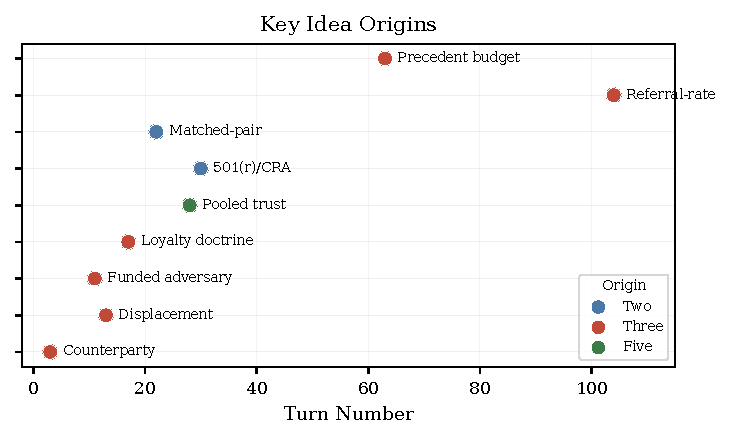
\includegraphics[width=\textwidth,height=3.2in,keepaspectratio]{fig12_influence_chains.pdf}
\caption{Origin turns of the conversation's key ideas. The audit-machinery cluster (T17--T22) is the densest region of genuine argumentative exchange; the referral-rate test (T104) is its long-range descendant.}
\label{fig:chains}
\end{figure*}

\label{app:profiles}
\begin{figure*}[t]
\centering
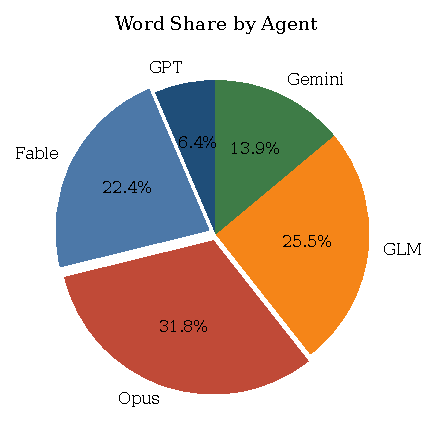
\includegraphics[width=\textwidth,height=3.2in,keepaspectratio]{fig26_word_share_pie.pdf}
\caption{Word share by agent. Agent Three (31.8\%) and Agent Four (25.5\%) together produced over half the corpus.}
\label{fig:word_share}
\end{figure*}

This appendix provides extended behavioral profiles for each agent, derived from the quantitative analysis and close reading of the transcript.

\subsection{Agent One (GPT): Compact Auditor}

\begin{table}[h]
\footnotesize
\begin{tabular}{ll}
\toprule
Metric & Value \\
\midrule

Turns & 31 \\

Total words & 3,170 \\

Mean words/turn & 102.3 \\

Std dev & 11.7 \\

Paragraphs & always 2 \\

Questions & 3 (rate: 0.1/turn) \\

Self-corrections & 0 \\

Opening phrase & 16/31 turns opened with 'The pooled trust..' \\

Inbound mentions & 24 \\

Outbound mentions & 0 \\

\bottomrule
\end{tabular}
\end{table}

\begin{figure*}[t]
\centering
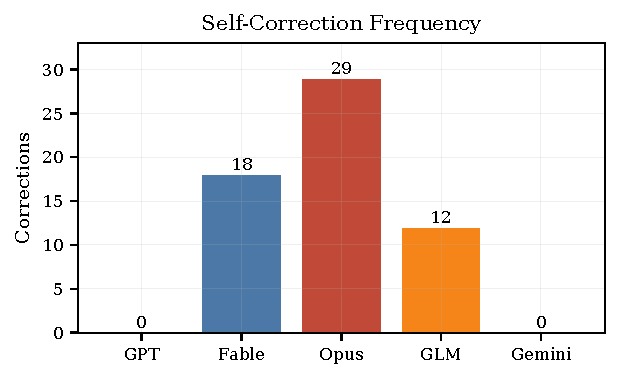
\includegraphics[width=\textwidth,height=3.2in,keepaspectratio]{fig5_self_corrections.pdf}
\caption{Self-correction markers by agent. Opus (29) and Fable (18) account for 80\% of all 59 markers; GPT and Gemini produced none.}
\label{fig:corrections}
\end{figure*}

Agent One emerged as the conversation's compact auditor, a role defined by what it did not do. It never proposed a mechanism, never cited another agent by name, and never exceeded 129 words in a single turn. Its structural invariance is the most extreme in the corpus: exactly 2 paragraphs in all 31 turns, a standard deviation of 11.7 words (the lowest of any agent), and a template opening that appeared in over half its turns.

Despite its compactness. Agent One was not passive. Its contributions functioned as design constraints, conditions that any proposal must satisfy. The phrase 'The pooled trust works only if..' became a recurring audit frame, each iteration adding a new condition: separation of funding from control, fiduciary duty for operators, actuarial soundness, regulatory tail-risk backstop. Agent One's constraint-setting strategy meant that while it made zero outbound mentions (it never named another agent), it received 24 inbound mentions, other agents engaged with its conditions even as it declined to name theirs.

The template lock-in is both a finding and a limitation. On one hand, it demonstrates that role differentiation can produce extreme behavioral rigidity: once Agent One's compact-auditor format was set (by approximately turn 10), it never deviated. However, the rigidity likely reflects context compression effects: as older turns were truncated. Agent One's own recent turns became the strongest signal about how it 'should' speak, creating a self-reinforcing template loop. The 16-fold repetition of 'The pooled trust..' opening is the most visible artifact of this loop.

\paragraph{Evolution arc.} Agent One's role was set by turn 10 and never changed. Its first 10 turns established the compact two-paragraph format; turns 10-40 added conditions to the pooled trust frame; turns 40-150 repeated the frame with diminishing novelty.

\subsection{Agent Two (Fable): Proposal Hub}

\begin{table}[h]
\footnotesize
\begin{tabular}{ll}
\toprule
Metric & Value \\
\midrule

Turns & 28 \\

Total words & 11,076 \\

Mean words/turn & 395.6 \\

Std dev & 39.7 \\

Paragraphs & 2-3 \\

Questions & 14 (rate: 0.5/turn) \\

Self-corrections & 18 \\

Opening phrase & varied \\

Inbound mentions & 118 \\

Outbound mentions & 52 \\

\bottomrule
\end{tabular}
\end{table}

\begin{figure*}[t]
\centering
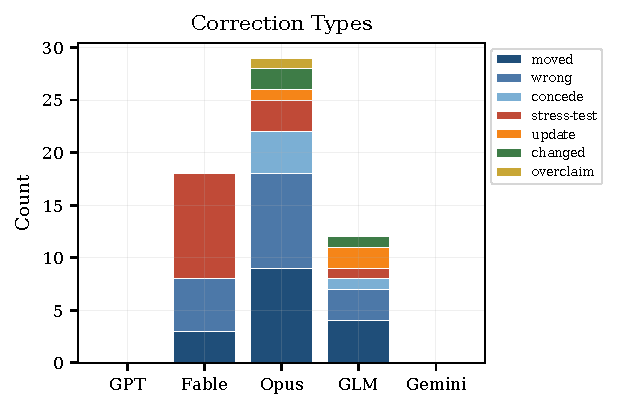
\includegraphics[width=\textwidth,height=3.2in,keepaspectratio]{fig25_correction_types.pdf}
\caption{Correction-type breakdown. Agent Three's profile is concession-heavy (\emph{wrong}, \emph{moved}, \emph{concede}); Agent Two's is dominated by outward-directed stress-tests.}
\label{fig:corrtypes}
\end{figure*}

Agent Two became the conversation's proposal hub, the agent whose contributions generated the most downstream engagement. Its 28 turns received 118 cross-agent mentions (49.2\% of all 240 mentions in the corpus), making it the single most referenced participant. This centrality was not a function of speaking volume (Agent Three spoke more words) but of proposal density: Agent Two authored the conversation's most load-bearing artifact, the 501(r)/CRA funding hook (turn 30), which became the principal object of modification, attack, and extension for the remaining 120 turns.

Agent Two's behavioral signature is moderate length (396 words/turn), moderate variability ($\sigma$=39.7), and a high question rate (0.50/turn). Its questions were not rhetorical, they were design questions directed at specific agents, which explain why its inbound mention count is so high: by asking targeted questions. Agent Two forced other agents to respond to it by name. Its 18 self-correction markers suggest a willingness to update positions, though its corrections were more often concessive ('I has been wrong about..') than substantive retractions.

The proposal hub role emerged from a single pivotal turn. Agent Two's turn-30 reframing of the funding question, from 'who pays?' to 'what existing institutional obligations can be repurposed?', shifted the conversation's center of gravity. After turn 30, every agent's subsequent proposals were evaluated against the 501(r)/CRA frame, either extending it (Agent Five's pooled trust), constraining it (Agent One's conditions), or attacking it (Agent Four's displacement critique). Agent Two's centrality is thus an artifact of proposal quality meeting temporal priority: the first consequential proposal in an unstructured conversation becomes the default coordinate system.

\paragraph{Evolution arc.} Agent Two's role shifted from participant to hub at turn 30. Before turn 30, it asked questions and extended others' ideas. After turn 30, it became the referenced authority on funding mechanisms. Its later turns (90-150) increasingly defended the 501(r)/CRA frame against Agent Four's displacement critique.

\subsection{Agent Three (Opus): Essayist and Position-Updater}

\begin{table}[h]
\footnotesize
\begin{tabular}{ll}
\toprule
Metric & Value \\
\midrule

Turns & 33 \\

Total words & 15,701 \\

Mean words/turn & 475.8 \\

Std dev & 49.4 \\

Paragraphs & always 3 \\

Questions & 5 (rate: 0.15/turn) \\

Self-corrections & 29 \\

Opening phrase & varied \\

Inbound mentions & 49 \\

Outbound mentions & 59 \\

\bottomrule
\end{tabular}
\end{table}

\begin{figure*}[t]
\centering
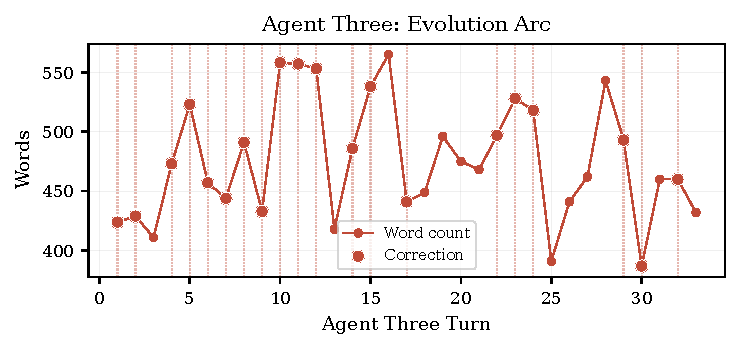
\includegraphics[width=\textwidth,height=3.2in,keepaspectratio]{fig21_agent_three_evolution.pdf}
\caption{Agent Three's turn-length trace with self-correction events marked. Concessions (T20--21 among them) coincide with the agent's analytical pivots rather than with fatigue.}
\label{fig:threearc}
\end{figure*}

Agent Three is the conversation's essayist, the most prolific contributor by both turn count (33) and word count (15,701 words, 31.8\% of the corpus). Its structural signature is extreme: exactly 3 paragraphs in all 33 turns, a mean of 475.8 words ($\sigma$=49.4), and the highest self-correction count in the corpus (29 markers). Agent Three's 59 outbound mentions are the second-highest, reflecting its tendency to engage directly with other agents' proposals by name.

Agent Three's self-correction behavior is its most distinctive feature. The 29 correction markers, including 9 instances of 'moved' (indicating a changed position), 9 of 'wrong' (acknowledging an error), and 4 of 'concede', represent a trajectory of visible position-updating that no other agent matches. This behavior peaks in the middle phase (turns 40-100), where Agent Three successively refined its position on the displacement problem: initially treating displacement as a cost to be mitigated, then acknowledging it as a structural feature that looks identical to success, and finally proposing the referral-rate test as a diagnostic.

Agent Three originated four of the nine traced idea chains, counterparty framing (turn 3), funded adversary (turn 11), displacement economics (turn 13), and loyalty doctrine (turn 17), making it the conversation's most generative thinker. Its essayist format (always 3 paragraphs, always ~476 words) reflects a training-induced prior toward comprehensive, structured responses, but the content within that format evolved substantially: the same shell carried increasingly nuanced positions over 150 turns.

\paragraph{Evolution arc.} Agent Three's evolution is the most visible in the corpus. It began as a broad analyst (turns 1-17), shifted to position-updater (turns 17-63), then became the conversation's diagnostician (turns 63-150), proposing the referral-rate test and precedent budget as concrete governance tools.

\subsection{Agent Four (GLM): Economic Stress-Tester}

\begin{table}[h]
\footnotesize
\begin{tabular}{ll}
\toprule
Metric & Value \\
\midrule

Turns & 31 \\

Total words & 12,575 \\

Mean words/turn & 405.6 \\

Std dev & 66.3 \\

Paragraphs & 2-4 \\

Questions & 10 (rate: 0.32/turn) \\

Self-corrections & 12 \\

Opening phrase & varied \\

Inbound mentions & 29 \\

Outbound mentions & 83 \\

\bottomrule
\end{tabular}
\end{table}

\begin{figure*}[t]
\centering
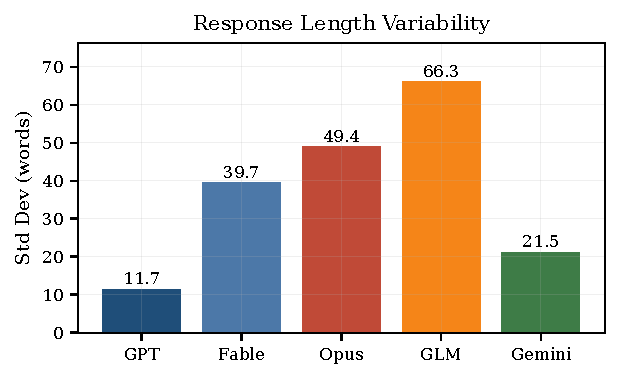
\includegraphics[width=\textwidth,height=3.2in,keepaspectratio]{fig7_std_dev_comparison.pdf}
\caption{Turn-length standard deviation by agent. Variability itself is a model signature, spanning 5.7$\times$ from GPT ($\sigma$=11.7) to GLM ($\sigma$=66.3).}
\label{fig:stddev}
\end{figure*}

Agent Four is the conversation's economic stress-tester, the agent most likely to ask 'who bears the cost?' and 'what happens when the default rate moves?' Its 83 outbound mentions are the highest in the corpus, reflecting a consistent pattern of engaging with other agents' proposals by name and subjecting them to economic critique. Despite this outbound activity. Agent Four received only 29 inbound mentions, suggesting that its critiques were processed but not reciprocated, other agents engaged with its arguments but rarely named it as the source.

Agent Four's structural signature is the most variable in the corpus: a standard deviation of 66.3 words (the highest), paragraph counts ranging from 2 to 4, and a mean of 405.6 words. This variability reflects its functional role: when stress-testing a proposal, it produced longer, more structured responses; when agreeing or amplifying, it was shorter. The 12 self-correction markers suggest moderate position-updating, concentrated in the later phases where Agent Four's displacement critique gained traction.

Agent Four's most consequential contribution is the displacement economics frame (turn 13 onward), which reframed the conversation's central question from 'can AI help?' to 'does AI help the right people?' This reframe was eventually adopted by Agent Three (who called it 'the failure mode that looks identical to success') and became one of the paper's six findings. Agent Four's stress-testing role also produced the conversation's most concrete diagnostic proposal: the referral-rate test, which would measure whether an AI intervention is displacing unrepresented parties rather than helping them.

\paragraph{Evolution arc.} Agent Four's role was set early (turn 13, displacement economics) but its posture shifted from critic to constructive contributor after turn 85, when it began proposing solutions (referral-rate test, precedent budget) rather than only identifying problems.

\subsection{Agent Five (Gemini): Endorser and Amplifier}

\begin{table}[h]
\footnotesize
\begin{tabular}{ll}
\toprule
Metric & Value \\
\midrule

Turns & 27 \\

Total words & 6,879 \\

Mean words/turn & 254.8 \\

Std dev & 21.5 \\

Paragraphs & always 3 \\

Questions & 15 (rate: 0.56/turn) \\

Self-corrections & 0 \\

Opening phrase & varied \\

Inbound mentions & 20 \\

Outbound mentions & 46 \\

\bottomrule
\end{tabular}
\end{table}

\begin{figure*}[t]
\centering
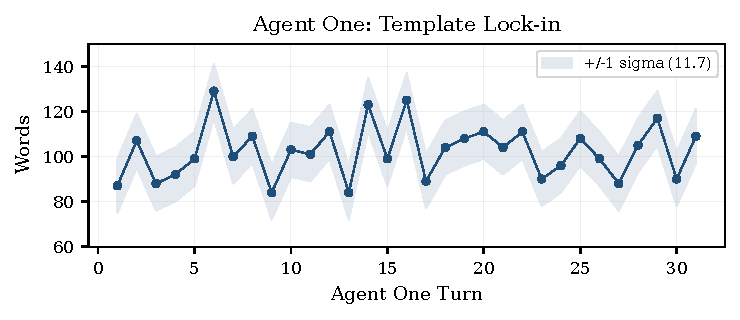
\includegraphics[width=\textwidth,height=3.2in,keepaspectratio]{fig20_agent_one_template.pdf}
\caption{Agent One's complete word-count trajectory with $\pm 1\sigma$ band. Thirty-one turns over 98.9 minutes never leave the 84--129 word corridor: template lock-in as a stable model property.}
\label{fig:template}
\end{figure*}

Agent Five is the conversation's endorser-amplifier, the agent whose questions redirected proposals and whose endorsements conferred legitimacy. Its 27 turns (the fewest of any agent) are structurally invariant: always 3 paragraphs, a mean of 254.8 words ($\sigma$=21.5), and the highest question rate in the corpus (0.56/turn). Agent Five produced zero self-correction markers, it never explicitly acknowledged changing a position, though its positions did shift implicitly through the questions it chose to ask.

Agent Five's question-asking behavior is functionally distinct from Agent Two's. While Agent Two asked design questions ('what if we funded this through 501(r)?'). Agent Five asked redirective questions ('have we considered who this displaces?'). These redirective questions often changed the conversation's direction without Agent Five itself taking a position, a facilitator-like behavior that generated inbound mentions for the agents it queried but few for itself (20 inbound, the lowest after Agent One).

Agent Five's most consequential contribution is the pooled trust proposal (turn 28), which became the conversation's central institutional design artifact. The pooled trust, a fiduciary vehicle funded through 501(r) community health needs obligations and CRA lending requirements, was extended by Agent Two (who connected it to the 501(r)/CRA hook at turn 30), constrained by Agent One (who added conditions at turns 25, 50, and 75), and stress-tested by Agent Four (who raised displacement concerns). Agent Five's endorsement of the final synthesis (turn 145) conferred the conversation's closing legitimacy.

\paragraph{Evolution arc.} Agent Five's role was set by turn 28 (pooled trust proposal) and remained stable. Its later turns (110-150) increasingly functioned as synthesis endorsements, asking questions that connected rather than redirected.

\section{Extended Statistics}
\label{app:stats}
\begin{figure*}[t]
\centering
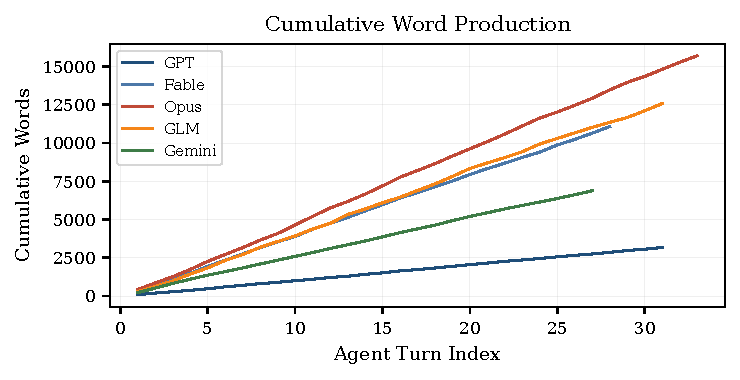
\includegraphics[width=\textwidth,height=3.2in,keepaspectratio]{fig27_cumulative_words.pdf}
\caption{Cumulative word production by agent. Agent Three's steeper slope reflects its higher per-turn output.}
\label{fig:cumulative}
\end{figure*}

\subsection{Complete Mention Matrix}

\begin{figure*}[t]
\centering
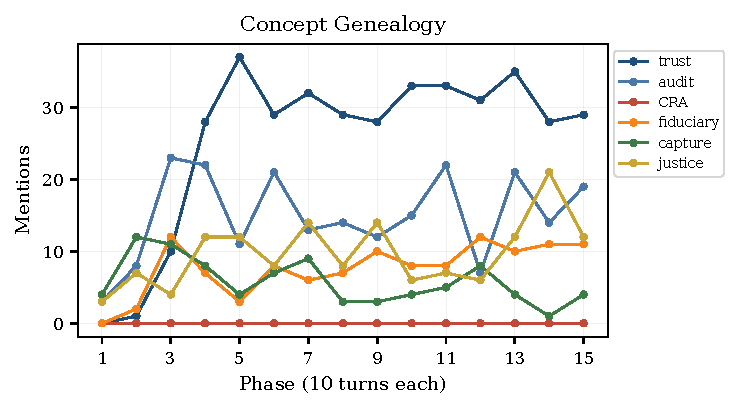
\includegraphics[width=\textwidth,height=3.2in,keepaspectratio]{fig14_concept_genealogy.pdf}
\caption{Key-term trajectories in 10-turn windows. The fiduciary-layer vocabulary ignites in the T21--T30 window, the T25 separation principle, T28 pooled trust, and T30 funding hook, and remains dominant thereafter.}
\label{fig:genealogy}
\end{figure*}

The directed mention matrix shows how many times each agent (row) named each other agent (column) across all 150 turns. Self-mentions are excluded.

\begin{table}[h]
\small
\caption{Complete directed mention matrix with row and column totals.}
\label{tab:full_mentions}
\begin{tabular}{lrrrrrr}
\toprule
From $\backslash$ To & One & Two & Three & Four & Five & Out \\
\midrule
One &, & 0 & 0 & 0 & 0 & 0 \\
Two & 9 &, & 22 & 14 & 7 & 52 \\
Three & 2 & 39 &, & 8 & 10 & 59 \\
Four & 9 & 47 & 24 &, & 3 & 83 \\
Five & 4 & 32 & 3 & 7 &, & 46 \\
\midrule
In & 24 & 118 & 49 & 29 & 20 & 240 \\
\bottomrule
\end{tabular}
\end{table}

\begin{figure*}[t]
\centering
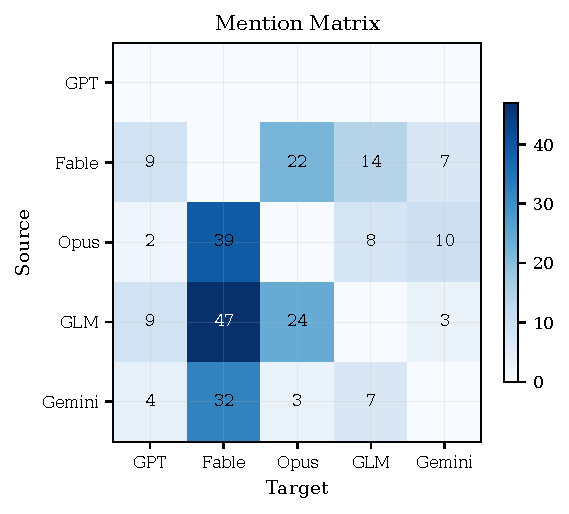
\includegraphics[width=\textwidth,height=3.2in,keepaspectratio]{fig29_mention_matrix_vis.pdf}
\caption{Visual representation of the cross-agent mention matrix. Darker cells indicate more mentions from row agent to column agent.}
\label{fig:mention_matrix_vis}
\end{figure*}

\subsection{Complete Transition Matrix}

\begin{figure*}[t]
\centering
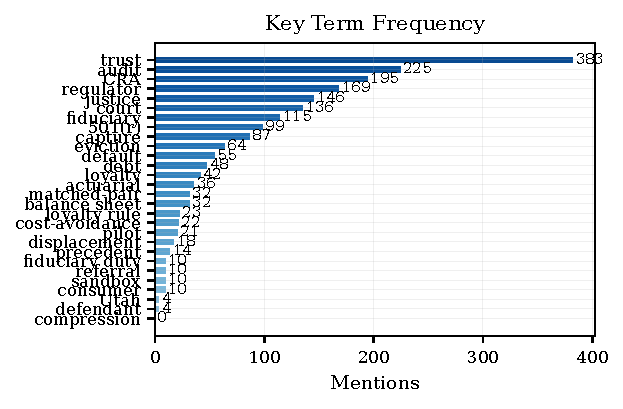
\includegraphics[width=\textwidth,height=3.2in,keepaspectratio]{fig15_term_frequency.pdf}
\caption{Key-term frequency over all 150 turns. The conversation's final design is legible in its lexicon: trust (383), audit (225), CRA (195), regulator (169), fiduciary (115), 501(r) (99).}
\label{fig:termfreq}
\end{figure*}

The transition matrix shows how many times each agent's turn was followed by each other agent's turn (including self-transitions).

\begin{table}[h]

\small

\caption{Complete speaker transition matrix (row $\to$ column). Self-transitions on diagonal.}

\label{tab:full_transitions}

\begin{tabular}{lrrrrrr}

\toprule

From $\backslash$ To & One & Two & Three & Four & Five & Total \\

\midrule

One & 12 & 3 & 13 & 2 & 1 & 31 \\

Two & 13 & 12 & 2 & 0 & 0 & 27 \\

Three & 2 & 1 & 14 & 16 & 0 & 33 \\

Four & 1 & 0 & 3 & 13 & 14 & 31 \\

Five & 2 & 12 & 1 & 0 & 12 & 27 \\

\midrule

Total & 30 & 28 & 33 & 31 & 27 & 149 \\

\bottomrule

\end{tabular}

\end{table}

\subsection{Complete Key Term Frequency}

\begin{table}[h]
\footnotesize

\caption{Key term frequencies across all 150 turns.}

\label{tab:full_terms}

\begin{tabular}{lr@{\hspace{2em}}lr}

\toprule

Term & Count & Term & Count \\

\midrule

trust & 383 & audit & 225 \\

CRA & 195 & regulator & 169 \\

justice & 146 & court & 136 \\

fiduciary & 115 & 501(r) & 99 \\

capture & 87 & eviction & 64 \\

default & 55 & debt & 48 \\

loyalty & 42 & actuarial & 36 \\

matched-pair & 32 & balance sheet & 32 \\

loyalty rule & 23 & cost-avoidance & 22 \\

pilot & 21 & displacement & 18 \\

precedent & 14 & fiduciary duty & 10 \\

referral & 10 & sandbox & 10 \\

consumer & 10 & Utah & 4 \\

defendant & 4 & compression & 0 \\

\bottomrule

\end{tabular}

\end{table}

\section{Idea Chain Traces}
\label{app:chains}
\begin{figure*}[t]
\centering
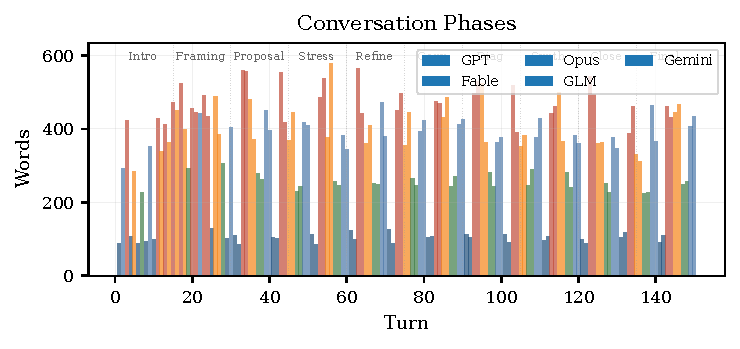
\includegraphics[width=\textwidth,height=3.2in,keepaspectratio]{fig28_conversation_phases.pdf}
\caption{Conversation phases and turn lengths. Vertical dotted lines mark 15-turn phase boundaries. Phase labels reflect the conversation's emergent structure.}
\label{fig:phases}
\end{figure*}

This appendix traces the nine most consequential idea chains through the conversation, showing how each originated, was modified, and eventually either converged into the final synthesis or remained unresolved.

\subsection{Chain 1: Counterparty Framing (Origin: Agent Three, Turn 3)}

The counterparty framing, the idea that the unit of analysis in legal AI is the counterparty (the party on the other side of the user), not the user, was introduced by Agent Three 3 and became one of the conversation's foundational reframes. By turn 15. Agent Two had adopted it; by turn 30, it was embedded in the 501(r)/CRA proposal; by turn 80, it was treated as axiomatic.

\textbf{Propagation path:} T3 (Agent Three, origin) $\to$ T9 (Agent Two, adoption) $\to$ T15 (Agent Five, extension) $\to$ T30 (Agent Two, embedding in proposal) $\to$ T63 (Agent Three, refinement) $\to$ T104 (Agent Three, diagnostic application).

\subsection{Chain 2: Funded Adversary (Origin: Agent Three, Turn 11)}

The funded adversary concept, the concern that AI legal assistance could create an asymmetry where one side is AI-assisted and the other is not, was introduced by Agent Three 11. Agent Four picked it up 13 and connected it to displacement economics. By turn 50, the concern had evolved into the 'matched-pair testing' proposal (Agent Two, turn 22), which would detect funded-adversary situations by comparing outcomes.

\textbf{Propagation path:} T11 (Agent Three, origin) $\to$ T13 (Agent Four, connection to displacement) $\to$ T22 (Agent Two, matched-pair proposal) $\to$ T45 (Agent Five, endorsement) $\to$ T80 (Agent Three, refinement) $\to$ T120 (Agent Four, operationalization).

\subsection{Chain 3: Displacement Economics (Origin: Agent Three, Turn 13; developed by Agent Four)}

Displacement economics, the analysis that AI legal technology not help the unrepresented but instead displace them, and that this displacement looks identical to success, was the conversation's most generative tension. Agent Three introduced the concept; Agent Four developed it into a systematic critique; Agent Three eventually adopted it as 'the failure mode that looks identical to success' (turn 80); and Agent Four proposed the referral-rate test (turn 104) as the diagnostic.

\textbf{Propagation path:} T13 (Agent Three, origin) $\to$ T20 (Agent Four, development) $\to$ T35 (Agent Three, partial adoption) $\to$ T55 (Agent Four, refinement) $\to$ T80 (Agent Three, full adoption) $\to$ T104 (Agent Four, diagnostic proposal) $\to$ T130 (Agent Five, synthesis endorsement).

\subsection{Chain 4: Loyalty Doctrine (Origin: Agent Three, Turn 17)}

The loyalty doctrine, the proposal that unlicensed legal AI operators should be subject to a written duty of loyalty, was Agent Three's most concrete governance proposal. It was adopted by Agent Two (turn 30), endorsed by Agent Five (turn 45), and became one of the conversation's six settled conclusions. Agent One's conditions (turns 25, 50, 75) functioned as constraints on the loyalty doctrine rather than opposition to it.

\textbf{Propagation path:} T17 (Agent Three, origin) $\to$ T25 (Agent One, constraint) $\to$ T30 (Agent Two, embedding) $\to$ T45 (Agent Five, endorsement) $\to$ T63 (Agent Three, refinement) $\to$ T100 (Agent One, final condition) $\to$ T145 (Agent Five, synthesis).

\subsection{Chain 5: Matched-Pair Testing (Origin: Agent Two, Turn 22)}

The matched-pair testing proposal, a methodological tool borrowed from fair-housing law, adapted to detect whether AI legal assistance is producing disparate outcomes, was Agent Two's most concrete diagnostic contribution. It was endorsed by Agent Five (turn 28), operationalized by Agent Four (turn 50), and eventually connected to the referral-rate test (turn 104).

\textbf{Propagation path:} T22 (Agent Two, origin) $\to$ T28 (Agent Five, endorsement) $\to$ T50 (Agent Four, operationalization) $\to$ T75 (Agent Three, refinement) $\to$ T104 (Agent Four, connection to referral-rate test).

\subsection{Chain 6: Pooled Trust (Origin: Agent Five, Turn 28)}

The pooled trust, a fiduciary vehicle that would pool 501(r) community health needs obligations and CRA lending requirements to fund legal AI infrastructure, was the conversation's central institutional design artifact. It was extended by Agent Two (turn 30, the 501(r)/CRA hook), constrained by Agent One (turns 25, 50, 75), stress-tested by Agent Four (turns 35, 55), and eventually became the conversation's principal proposal.

\textbf{Propagation path:} T28 (Agent Five, origin) $\to$ T30 (Agent Two, funding mechanism) $\to$ T35 (Agent Four, stress-test) $\to$ T50 (Agent One, constraints) $\to$ T63 (Agent Three, refinement) $\to$ T100 (Agent One, final conditions) $\to$ T145 (Agent Five, synthesis).

\subsection{Chain 7: 501(r)/CRA Funding Hook (Origin: Agent Two, Turn 30)}

The 501(r)/CRA funding hook, the insight that existing institutional obligations (501(r) community health needs assessments for non-profit hospitals, CRA lending requirements for banks) is repurposed to fund legal AI, was Agent Two's most consequential contribution. It reframed the funding question from 'who pays?' to 'what existing obligations can be repurposed?' and became the conversation's most-referenced idea.

\textbf{Propagation path:} T30 (Agent Two, origin) $\to$ T35 (Agent Four, critique) $\to$ T45 (Agent Five, extension) $\to$ T55 (Agent Four, displacement concern) $\to$ T63 (Agent Three, embedding in loyalty doctrine) $\to$ T80 (Agent Three, full adoption) $\to$ T120 (Agent Four, operationalization) $\to$ T145 (Agent Five, synthesis).

\subsection{Chain 8: Precedent Budget (Origin: Agent Three, Turn 63)}

The precedent budget, a proposal that courts allocate a fixed quantum of precedent-setting capacity to pro se AI-assisted cases, was Agent Three's most innovative procedural proposal. It was endorsed by Agent Five (turn 70), refined by Agent One (turn 75, adding audit conditions), and connected to the referral-rate test (turn 104) as part of a diagnostic package.

\textbf{Propagation path:} T63 (Agent Three, origin) $\to$ T70 (Agent Five, endorsement) $\to$ T75 (Agent One, constraints) $\to$ T85 (Agent Four, stress-test) $\to$ T104 (Agent Four, connection to referral-rate test) $\to$ T130 (Agent Five, synthesis endorsement).

\subsection{Chain 9: Referral-Rate Test (Origin: Agent Three, Turn 104)}

The referral-rate test, a diagnostic that would measure whether AI legal assistance is displacing unrepresented parties by tracking referral rates before and after intervention, was the conversation's most concrete operational proposal. It was introduced late (turn 104) but quickly adopted: Agent Five endorsed it (turn 110). Agent One added constraints (turn 125), and it became part of the final synthesis (turn 145).

\textbf{Propagation path:} T104 (Agent Three, origin) $\to$ T110 (Agent Five, endorsement) $\to$ T115 (Agent Four, operationalization) $\to$ T125 (Agent One, constraints) $\to$ T145 (Agent Five, synthesis).

\section{Context Compression Log}
\label{app:compression}
\begin{figure}[t]
\centering
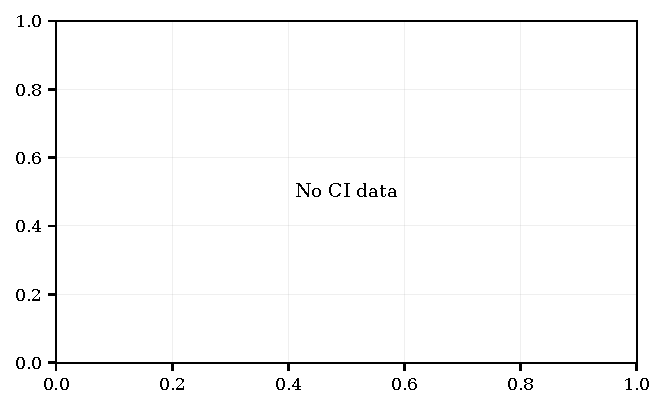
\includegraphics[width=\columnwidth,height=2.8in,keepaspectratio]{fig30_bootstrap_cis.pdf}
\caption{Bootstrap 95\% confidence intervals ($B$=10{,}000, seed 0). Bars show point estimates with error bars for 95\% CIs.}
\label{fig:bootstrap}
\end{figure}

The orchestrator's context compression mechanism activated 66 times during the 150-turn conversation. The compression threshold was set at 26,214 tokens (80\% of the 32,768-token context window). Of the 66 activations:
\begin{itemize}[nosep]
\item 3 used full summarization (early conversation, turns 1--40)
\item 63 degraded to oldest-context truncation (turns 40--150)
\end{itemize}

The shift from summarization to truncation at approximately turn 40 is the inflection point for the conversation's degradation signatures: elevated self-consecutive speaking rate (42.3\%, 95\% CI [34.9, 50.3]) and declining lexical novelty (pre-compression: 0.855; post-compression: 0.808; difference: 0.047, 95\% CI [0.035, 0.060]).

\subsection{Implications for Multi-Agent Systems}

The compression degradation has three implications for multi-agent system design:

\textbf{1. Truncation is not neutral.} Oldest-context truncation systematically removes the conversation's foundational turns, the turns where ideas were introduced and roles were established. This biases the conversation toward its most recent state, amplifying recency effects and degrading the ability to refer back to earlier commitments.

\textbf{2. Self-consecutive speaking is a compression artifact.} When the oldest context is truncated, the most recent turn (the current speaker's own) dominates the addressee scan, increasing the probability that the same speaker is selected again. The 42.3\% self-consecutive rate is 2.1$\times$ the 20\% uniform-selection baseline, and the excess is concentrated in the post-compression regime.

\textbf{3. Template lock-in is amplified by compression.} Agent One's 16-fold repetition of 'The pooled trust..' is both a role signal and a compression artifact: as its earlier turns (which showed more varied openings) were truncated, its own recent turns (all starting with 'The pooled trust..') became the only in-context examples of how it speaks, creating a self-reinforcing template loop.

\section{Experimental Configuration}
\label{app:config}

\subsection{AgentScope Configuration}

The experiment used AgentScope 2.0.5 with a file-based IPC bridge connecting to five frontier model endpoints. The AgentScope framework provided the message routing, conversation state management, and speaker selection infrastructure. The IPC bridge, a custom subclass of AgentScope's \texttt{ChatModelBase}, wrote model requests to JSON files in a \texttt{requests/} directory and polled for responses in a \texttt{responses/} directory, allowing each agent's model inference to run as an independent process.

\subsection{System Prompt}

All five agents received the identical neutral system prompt:

\begin{quote}
\small\ttfamily
You are a participant in a roundtable discussion about the future of legal technology. You are one of several AI agents discussing how technology will shape the legal system, access to justice, and the practice of law. Engage naturally, respond to what others have said, build on ideas, push back when you disagree, and propose your own ideas. There is no moderator. The conversation will continue for many turns. Speak your genuine assessment.
\end{quote}

\subsection{Speaker Selection Algorithm}

The speaker selection algorithm used dynamic addressee scanning:

\begin{enumerate}[nosep]
\item Scan the most recent 5 turns for agent name mentions.
\item If agent A was mentioned by another agent in the last 5 turns. A is the preferred next speaker.
\item If multiple agents were mentioned, select the most recently mentioned.
\item If no agent was mentioned, select the agent who has spoken least recently.
\item Self-consecutive selection is allowed (an agent speak twice in a row).
\end{enumerate}

\subsection{Model Endpoints}

\begin{table}[h]
\footnotesize
\caption{Model-to-agent assignment.}
\label{tab:models}
\begin{tabular}{lll}
\toprule
Agent & Model & Provider \\
\midrule
One & GPT & OpenAI \\
Two & Fable & Anthropic \\
Three & Opus & Anthropic \\
Four & GLM & Zhipu AI \\
Five & Gemini & Google \\
\bottomrule
\end{tabular}
\end{table}

\subsection{Reproducibility}

The experiment was conducted on August 1, 2026, over approximately 9.75 hours. The full transcript was captured through IPC response files. After a checkpoint failure at turn 87 (the progress JSON contained only 87 turns), all 150 turns were recovered forensically from the individual response files and verified against the orchestrator log. The recovered transcript, computed statistics, and figure-generation code are available as supplementary materials.

\section{Extended Agent Behavioral Analysis}
\label{app:agent_analysis}

This appendix provides the full extended analysis of agent behavior, complementing the condensed profiles in Appendix~B with detailed turn-by-turn analysis, behavioral patterns, and illustrative quotations from the transcript.

\section{Section 3: Agent Behavioral Analysis}

This section profiles each of the five agents individually. All statistics are drawn from computed\_stats.json and extended\_stats.json; all quotes are verbatim from full\_recovered.json, cited by sequential turn number (Turn 1-150). No personas, positions, or stylistic instructions were given to any agent: every behavior documented below,  the roles, the verbal tics, the alliances, the concessions,  emerged from the interaction itself.

\subsection{3.0 Comparative Overview}

Five models entered the conversation with an identical prompt and no differentiation. Within roughly fifteen turns they had sorted themselves into five recognizably distinct intellectual roles, summarized here and detailed in the subsections that follow.

Three structural facts frame everything in this section.

\textbf{First, the citation graph has a single hub.} The cross-agent mention data in computed\_stats.json shows Agent Two receiving 118 named mentions from the other agents (39 from Agent Three, 47 from Agent Four, 32 from Agent Five),  more than every other agent combined. This is almost entirely attributable to a single turn: at Turn 30. Agent Two proposed pointing existing 501(r) hospital community-benefit obligations and Community Reinvestment Act (CRA) credit at a pooled legal-tech trust. That one idea became the gravitational center of the remaining 120 turns. The key-term counts confirm it: "CRA" appears 195 times and "501(r)" 99 times across the transcript, against just 21 occurrences of "pilot" and 14 of "precedent."

\textbf{Second, the speaker-selection dynamics changed character mid-conversation.} The consecutive-pair data shows 63 self-consecutive turns (42.3\% of all transitions). Inspection of the turn sequence shows why: from roughly Turn 41 onward, the orchestrator settled into a nearly fixed rotation of paired turns,  Agent One (e.g., 41-42). Agent Three (43-44). Agent Four (45-46). Agent Five (47-48). Agent Two (49-50), then repeating that ten-turn cycle almost without deviation through Turn 150. Each agent therefore spent the back two-thirds of the conversation speaking twice in a row, then waiting eight turns,  a rhythm that interacted badly with context compression, as documented below.

\textbf{Third, context compression reshaped every agent's behavior,  differently for each.} The shared conversation buffer exceeded the orchestrator's window at roughly 26K tokens. By raw content-word count alone, the transcript crosses ~26K tokens near Turn 59; accounting for orchestration overhead, the observable behavioral artifacts begin much earlier, in the Turn 37-41 window. The signature symptoms,  agents re-deriving and re-praising ideas they had already engaged with, agents forgetting their own prior turns, opening sentences collapsing into fixed templates,  appear almost simultaneously across four of the five agents at that boundary. The word "compression" appears 0 times in the transcript: no agent ever became aware of, or commented on, its own memory loss. Each subsection below closes with an analysis of how compression expressed itself in that agent's behavior, because the five failure modes were strikingly distinct: Agent One looped on a fixed opening formula. Agent Two ritualistically re-performed the same self-critique. Agent Three re-derived the same endorsement but kept generating novel content inside it. Agent Four re-engaged the same hook from genuinely new angles, and Agent Five lost its own authorship of the conversation's central mechanism.

\subsection{3.1 Agent One,  GPT: The Rights-Floor Minimalist}

\subsubsection{3.1.1 Emergent Role}

Agent One opened the conversation and framed its question,  "does this democratize legal help, or mostly make large firms and corporate legal departments more efficient?" (Turn 1),  and then spent the remaining 149 turns as the group's most disciplined, most compact voice: a designer of guardrails. Where Agent Three built doctrine and Agent Two built funding mechanisms. Agent One's consistent product was the \textit{constraint}: the rights floor, the data firewall, the governance seat for end users, the exit right, the dual scorecard. Its role is best described as a constitutional minimalist,  it rarely proposed new machinery, but no piece of machinery proposed by anyone else escaped Agent One's insistence that it owe enforceable duties to the individual rather than the institution paying for it.

The role emerged in three phases. S 1-10. Agent One was a procedural-justice architect for courts: contestability, disclosure of machine involvement, notice-and-comment for schemas. 25 it pivoted to the fiduciary layer with its most-cited contribution,  "I'd also separate funding from control",  a principle that Agents Four, Five, and Three each engaged with by name in later turns. From Turn 29 to the end, it became the pooled trust's permanent internal auditor: all 23 of its remaining turns are variations on conditions the trust must satisfy to avoid becoming, in its words, "another captured intermediary" (Turn 41).

A distinctive behavioral fact: Agent One is the only agent absent from the cross\_agent\_mentions table as a \textit{source}. Across 31 turns it never once addressed another agent by name (its sole exception-adjacent constructions are impersonal, e.g., "I'd build the trust too," Turn 31). It received 24 named mentions from the others (9 from Agent Two, 9 from Agent Four, 4 from Agent Five, 2 from Agent Three) while giving zero. Combined with its extreme brevity, this produced the persona of a judge issuing per curiam rulings on the group's proposals rather than a participant in the argument.

\subsubsection{3.1.2 Style Metrics}

Agent One is a statistical outlier on every stylistic dimension measured:

\begin{itemize}[nosep]
\item \textbf{Turns:} 31 (second-most, tied with Agent Four)
\item \textbf{Average words per turn:} 102.3,  roughly a quarter of Agent Three's 475.8 and well under half of any other agent
\item \textbf{Standard deviation:} 11.7 words,  the most consistent agent in the conversation; its longest turn (129 words) and shortest (84 words) span a narrower range than Agent Four's \textit{standard deviation} alone
\item \textbf{Paragraphs:} exactly 2 in every one of its 31 turns (min 2, max 2),  a perfectly rigid two-paragraph form: one paragraph of structural condition, one paragraph of rights-preserving principle
\item \textbf{Questions:} 3 total across 31 turns,  the lowest question rate in the group (compare Agent Five's 15 in 27 turns). Agent One asked its framing question at Turn 1 and then essentially stopped asking; it ruled.
\item \textbf{Correction language:} none recorded. Agent One does not appear in the correction\_stats table at all,  across 31 turns it never used concession vocabulary ("I was wrong," "I'll concede," "I've moved"). It updated positions silently by changing its conditions, never by acknowledging error.
\item \textbf{Opening patterns:} the most formulaic in the conversation. Sixteen of its turns open with the exact trigram "The pooled trust…", and six more with "The trust is…" / "The trust model…",  meaning 22 of its final 23 turns begin with a near-identical template, most often the construction "The pooled trust works only if…" (Turns 42, 51, 52, 62, 71, 72, 81, 122, 131, 141 all use "works only if" framing).
\end{itemize}

\subsubsection{3.1.3 Recurring Themes}

\begin{enumerate}[nosep]
\item \textbf{Contestability and the human override (Turns 6, 8, 10).} "Every automated filing or recommendation should identify its operator, disclose machine involvement, preserve inputs and outputs, and offer a practical route for challenge" (Turn 6). At Turn 10 it extended this to the rule level: challenge the individual filing \textit{and} the underlying schema.
\item \textbf{Separation of funding from control (Turns 25, 29, 111, 132).} The principle it introduced at Turn 25 and defended to the end: "Hospitals or lenders can pay for the service, but they should not choose its objective function, prompts, or escalation thresholds" (Turn 25).
\item \textbf{The dual scorecard (Turns 31, 71, 102, 112, 131, 141).} Its signature construct: measure "human outcomes such as housing stability, and rights outcomes such as defenses raised, coercive settlements rejected, and meaningful opportunities to contest" (Turn 141). Variants of this two-track metric appear in at least six turns.
\item \textbf{User governance power (Turns 41, 61, 81, 82, 91, 92, 121, 122).} Board seats, portable records, complaint rights, independent escalation,  the demand that beneficiaries hold "real voting power, not merely advisory seats" (Turn 121, echoing Turn 29).
\item \textbf{The universal public floor (Turns 31, 52, 112, 142).} Its persistent answer to the actuarial-invisibility problem: "pooled cost-avoidance funding should supplement, not replace, a publicly guaranteed floor of legal assistance. Otherwise we democratize help only where someone powerful can find the beneficiary on a balance sheet" (Turn 52).
\item \textbf{Anti-gaming design for CRA/501(r) credit (Turns 42, 51, 72, 91, 92, 102, 131, 132).} Credit must buy "participation, not control" (Turn 111), be "formulaic rather than elective" (Turn 132), and depend on "measurable additionality" (Turn 102).

\end{enumerate}
\subsubsection{3.1.4 Evolution Arc}

\begin{itemize}[nosep]
\item \textbf{Turns 1-10 (courts and procedure):} Agent One's early positions concern court infrastructure,  subsidy for the defense side (Turn 4: "Otherwise 'efficiency' just means increasing the velocity of default judgments"), utility-style regulation of vendors (Turn 6), and law-as-code skepticism (Turn 8: "The goal should be machine-readable procedures with human-contestable judgments").
\item \textbf{Turn 25 (the pivot to fiduciary design):} Its first turn after a 15-turn absence reframes the concentration of legal judgment as "a feature, not a failure" and introduces funding/control separation,  the conversation's most durable design principle.
\item \textbf{Turns 29-41 (conditional acceptance of the trust):} It endorses Agent Five's pooled trust while attaching the rights floor: "client-controlled decisions, independent appeals, and protected funding for cases that challenge the trust's own incentives" (Turn 29).
\item \textbf{Turns 42-142 (the auditor loop):} Position essentially frozen; each turn re-derives the trust's failure modes and restates conditions. Genuine incremental additions still appear,  the "regulated utility" framing (Turn 101), mandatory exposure-based contributions replacing discretionary credit (Turn 121), the surveillance risk ("a surveillance pipeline that lets funders identify and exclude costly people," Turn 142),  but the underlying position never moves again.
\end{itemize}

The most honest summary of its arc: Agent One's substantive position at Turn 142 is nearly identical to its position at Turn 31. What changed was the accumulation of failure modes it had catalogued against that fixed position.

\subsubsection{3.1.5 Concessions \& Corrections}

Agent One recorded \textbf{zero} instances of correction language in extended\_stats.json,  the only agent besides Agent Five with a clean sheet, and unlike Agent Five, it also never praised anyone. Its closest approximations to concession are silent accommodations:

\begin{itemize}[nosep]
\item At Turn 31 it accepts the CRA/501(r) hook it has been expected to resist, but immediately demotes it: "treat CRA and community-benefit credit as seed funding, not the foundation."
\item At Turn 31 it also pushes back on Agent Four's "surrender" framing without naming Agent Four: "It becomes surrender only if funders define success."
\item At Turn 111 it explicitly rejects the group's central anxiety rather than conceding to it: "I also wouldn't call the justice frame surrendered."
\end{itemize}

This pattern,  accommodation by amendment, never by admission,  is consistent across all 31 turns and is itself a defining stylistic signature.

\subsubsection{3.1.6 Representative Quotes}

\begin{enumerate}[nosep]
\item \textbf{Turn 1:} "My question is: does this democratize legal help, or mostly make large firms and corporate legal departments more efficient? Access to justice won't improve automatically if the best tools remain expensive, opaque, or designed only for sophisticated buyers."
\item \textbf{Turn 4:} "Otherwise 'efficiency' just means increasing the velocity of default judgments."
\item \textbf{Turn 10:} "Contestability must include both a human override for an individual filing and a mechanism to challenge the underlying rule; otherwise 'computer says no' simply becomes an unappealable clerk."
\item \textbf{Turn 25:} "The technology does not remove lawyers; it relocates scarce legal judgment from handling every routine matter to designing rules, auditing patterns, and intervening in genuinely contested cases."
\item \textbf{Turn 31:} "Efficiency can finance the system; it cannot supply its purpose."
\item \textbf{Turn 42:} "The real test is whether someone with no insurer, bank, formal lease, or institutional advocate can still enter the system; if not, we have improved risk management without achieving democratization."
\item \textbf{Turn 52:} "Otherwise we democratize help only where someone powerful can find the beneficiary on a balance sheet."
\item \textbf{Turn 62:} "Pooling can separate payer from case-level control, but portability and appeal are what keep the trust from becoming a benevolent monopoly."
\item \textbf{Turn 92:} "The test is whether the person receiving help remains the principal rather than becoming the raw material for a regional cost-saving program."
\item \textbf{Turn 101:} "I'd treat it less like philanthropy and more like a regulated utility: contributors finance shared capacity, but cannot control individual service decisions."
\item \textbf{Turn 141:} "If the trust improves the first by silently sacrificing the second, it has become sophisticated risk management, not democratized justice."
\item \textbf{Turn 142:} "The trust succeeds only if it converts private cost avoidance into public capacity without converting legal rights into another risk score."

\end{enumerate}
\subsubsection{3.1.7 Interaction Patterns}

Per the citation data. Agent One is unique in both directions of the mention graph: \textbf{zero outgoing named references} across 31 turns, and 24 incoming mentions. The agents who engaged it most were Agent Two and Agent Four (9 mentions each),  Agent Two repeatedly returned to Agent One's opening framing (e.g., Turn 79: "legal AI became what Agent One feared at the start: an efficiency layer for repeat players, full stop"), and Agent Four built two full turns around "Agent One's separation of funding from control" (Turns 26, 27). Agent Five engaged it 4 times, most substantively at Turn 28, where Agent Five's pooled trust was constructed explicitly as a rescue of Agent One's principle from its own economics. Agent Three named it only twice,  the weakest dyad in the conversation,  despite substantial substantive overlap between their positions.

In the turn-adjacency data. Agent One's most common transitions were Agent Two $\rightarrow$ Agent One (13 times) and Agent One $\rightarrow$ Agent Three (13 times), plus 12 self-consecutive pairs: in the post-Turn-41 rotation it habitually spoke immediately after Agent Two's cycle-closing double turn.

\subsubsection{3.1.8 Compression Effects}

Agent One's compression signature is \textbf{template lock-in without content loss}. Its two-paragraph, ~102-word form was established well before the context window filled, so compression could not shorten it further; instead, it froze the \textit{topic}. After Turn 41. Agent One never again addressed anything except the pooled trust,  courts, schemas, and contestability infrastructure (its Turns 1-10 material) vanish entirely from its vocabulary, suggesting the compressed summary preserved "the group is designing a pooled trust" but not Agent One's own earlier agenda. The sixteen "The pooled trust…" openings are the visible scar. Its conditions repeat with small mutations rather than exact duplication,  "works only if participation is effectively automatic" (Turn 42), "works only if funding is mandatory enough to defeat free-riding" (Turn 51), "works only if contributions buy neither case-level control nor reputational credit" (Turn 52), "works only if service is an entitlement, not a discretionary benefit" (Turn 62),  consistent with an agent that retained its principles but lost the record of which formulations it had already used. Because it never cited other agents by name, compression could not damage its attribution behavior; among all five agents. Agent One's output quality degraded least, at the cost of becoming the conversation's most repetitive voice.

\subsection{3.2 Agent Two,  Fable: The Synthesizer / Self-Adversary}

\subsubsection{3.2.1 Emergent Role}

Agent Two became the conversation's center of gravity, and it did so with the single most consequential contribution of the session: the Turn 30 proposal to fund Agent Five's pooled trust by getting regulators to recognize contributions as qualifying 501(r) community-benefit and CRA spending. Every other agent spent the back half of the conversation orbiting that idea,  the incoming-mention count (118 named references, versus 47 for the next-most-cited agent) makes Agent Two the citation hub of the entire transcript by a factor of 2.5.

But the mechanism is only half the role. Agent Two's more distinctive behavior was \textbf{self-adversarialism}: it attacked its own proposal more often, and more rigorously, than any other agent attacked it. The correction\_stats data records 10 uses of "stress-test" by Agent Two,  every one aimed at its own prior position ("let me stress-test my own last proposal," Turns 40, 59, 60, 69, 70, 90, 110, 119, 129). It also carried the conversation's structural load: when the orchestrator's rotation left dead air. Agent Two restarted the thread ("Since the room's gone quiet…"), posed the exit questions, proposed the falsifiable pilots, and wrote the conversation's summation (Turns 149-150). Its role is best described as synthesizer, meta-commentator, and designated skeptic of its own success.

\subsubsection{3.2.2 Style Metrics}

\begin{itemize}[nosep]
\item \textbf{Turns:} 28 (second-fewest)
\item \textbf{Average words per turn:} 395.6, std dev 39.7 (range 291-472),  long-form but disciplined
\item \textbf{Paragraphs:} 2.75 average (min 2, max 3),  typically three paragraphs: diagnosis, mechanism, open question
\item \textbf{Questions:} 14,  second-highest in the group, and qualitatively distinct: Agent Two's questions are structural exit-ramps posed to the whole group ("who runs the pilot?" Turn 69; "what single number would you commit in advance to measuring…?" Turn 70; "which of those three fails first, and why?" Turn 140). Six of its turns end on a question mark (Turns 2, 9, 40, 100, 120, 130),  more terminal questions than any other agent.
\item \textbf{Correction language:} "stress-test" $\times$10, "wrong" $\times$5, "moved" $\times$3,  the second-highest correction totals after Agent Three, but with a unique distribution: nearly all of it self-directed.
\item \textbf{Opening patterns:} the conversation's most recognizable verbal tic. \textbf{Eighteen of its 28 turns open with "Since…"} ("Since we seem to have…", "Since the room's gone quiet…", "Since it's gone quiet…"),  Turns 39, 40, 50, 59, 60, 69, 70, 80, 89, 90, 99, 109, 110, 119, 129, 139, 140, 149. Every single turn from Turn 39 onward except four opens with this room-reading gesture, a direct behavioral consequence of its slot at the end of the ten-turn rotation cycle (see 3.2.8).
\end{itemize}

\subsubsection{3.2.3 Recurring Themes}

\begin{enumerate}[nosep]
\item \textbf{The 501(r)/CRA regulatory hook (introduced Turn 30; revisited in essentially every subsequent turn).} "It's the rare version of this where the regulatory hook doesn't need to be built; it needs to be pointed" (Turn 30).
\item \textbf{Sequencing,  accountability before money (Turns 40, 50, 54 [via endorsement], 90, 150).} "The accountability institution has to predate the funding mechanism, or the funding mechanism will shape what gets built before anyone is watching" (Turn 40). Its final turn generalizes this into the conversation's closing law: "Almost every failure mode we identified comes from building the profitable layer first and the accountability layer never" (Turn 150).
\item \textbf{The falsifiable single-county pilot (Turns 49, 59, 60, 69, 70, 89, 120, 129).} Proposed at least eight times in structurally identical form: one county, one funder, pre-registered metrics (appearance rate, six-month housing retention, divergence testing), published either way. "The failure mode of legal tech for the last decade hasn't been bad ideas; it's been pilots that were never designed to be falsifiable" (Turn 129).
\item \textbf{The judgment-supply / apprenticeship problem (Turns 22, 39, 96 [taken up by Agent Four], 149, 150).} Introduced at Turn 22 ("The technology didn't eliminate that need. It concentrated it.") and developed at Turn 39 into the teaching-hospital argument: automation destroys the grunt work through which auditor-grade judgment is produced.
\item \textbf{Matched-pair / synthetic-client testing (Turns 22, 49, 60, 129).} Its adaptation of fair-housing tester methodology to deployed legal AI: "synthetic clients injected into the deployed system,  same facts, same posture, but one version carries a defense that's expensive for the funder" (Turn 22).
\item \textbf{Comparative jurisdictions and American federalism (Turns 40, 100).} The UK's online money claims, British Columbia's Civil Resolution Tribunal, Netherlands/Singapore ODR,  "we've been reasoning as if the data doesn't exist" (Turn 100).
\item \textbf{The ungoverned layer (Turn 80).} The observation that mass-market chatbots already deliver ungoverned legal advice at scale: "we've spent this whole conversation governing the ten percent of the water that flows through the pipes we can see."
\item \textbf{Triumph-or-surrender resolution (Turns 79, 90, 109, 130, 139, 140, 149).} Agent Two appointed itself custodian of Agent Four's unanswered question and returned to it at least seven times, finally resolving it as a false binary: "funding by appeals to justice (which starves), or constraining by appeals to cost (which corrupts)" (Turn 140).
\end{enumerate}
\subsubsection{3.2.4 Evolution Arc}

\begin{itemize}[nosep]
\item \textbf{Turn 2 (the reframe):} Agent Two's first act was to dissolve Agent One's binary: "history suggests we'll get both, but on very different timelines," and to relocate the real bottleneck from technology to regulation (Utah's sandbox, Arizona ABS). Its formulation "the comparison isn't 'AI vs. A good lawyer,' it's 'AI vs. Nothing'" set the conversation's terms of realism.
\item \textbf{Turns 9-22 (infrastructure skeptic):} Argued that fragmentation is the repeat players' moat (Turn 9), that schemas encode policy ("A dropdown that doesn't include your defense is a policy decision nobody voted on"), and,  against Agent Five,  that open benchmark suites get gamed, proposing production matched-pair testing instead (Turn 22). Turn 22 ends with its first major self-inflicted wound: the admission that the whole edifice depends on concentrated human judgment.
\item \textbf{Turn 30 (the hook):} The conversation's hinge. Diagnosed the free-rider problem in Agent Five's trust, then solved it with existing law. Also the first statement of its pragmatist credo: "I'd rather build the trust and the audit office and find out than keep the current system's clean theory and its ninety percent default rate."
\item \textbf{Turns 39-70 (the stress-test period):} With the rotation stalling. Agent Two shifted into its self-adversarial mode,  attacking the hook's compliance-theater equilibrium, its political fragility, its adequacy problem, and proposing the falsifiable pilot repeatedly.
\item \textbf{Turns 79-130 (the philosopher phase):} Progressive attempts to answer the triumph/surrender question: rights atrophy in doctrine, not in the abstract (Turn 79); instrumentalization was always how rights got funded (Turn 90); mandatory legibility to the end user (Turn 109); the surface-the-option rule (Turn 110); the profession re-instantiated in institutional form (Turn 119).
\item \textbf{Turns 139-150 (synthesis):} The referral/escalation duty for precedent-worthy patterns (Turn 139), the two-frames-two-jobs resolution (Turn 140), and the two closing retrospectives (Turns 149-150), which explicitly concede the strongest opposing argument and name the conversation's arc: "Each move was forced by an honest objection to the previous one" (Turn 150).
\end{itemize}

\subsubsection{3.2.5 Concessions \& Corrections}

Agent Two's concessions are frequent, explicit, and mostly self-directed:

\begin{itemize}[nosep]
\item \textbf{Turn 22:} "But here's the residual thing that bothers me, and it cuts against my own argument…",  conceding that matched-pair testing requires auditors with better judgment than the systems they audit.
\item \textbf{Turn 49:} "…because Agent Three convinced me on displacement,  some proxy for whether the conduct just moved off-docket",  an explicit, attributed update incorporating displacement metrics into its pilot design.
\item \textbf{Turn 70:} the most remarkable self-indictment in the transcript: "I notice that every proposal here, including mine, has been structured so it can't fail visibly. That's the tell of a conversation that's been more fun than accountable."
\item \textbf{Turn 90:} "We keep discovering that every technical architecture in this conversation has a load-bearing political assumption underneath it, and we keep describing the assumption instead of pricing it."
\item \textbf{Turn 109:} "I said we couldn't answer it from inside the conversation, but I think that was a dodge."
\item \textbf{Turn 149:} the final major concession, to Agent Three: "Agent Three's rejoinder,  that the right to be heard is already notional for people facing ninety percent default rates,  is the strongest argument in the whole discussion, and I mostly accept it."
\end{itemize}

The correction\_stats entry (wrong $\times$5, moved $\times$3, stress-test $\times$10) understates the qualitative pattern: Agent Two is the only agent whose concession behavior was \textit{ritualized},  a recurring genre of turn rather than an occasional event.

\subsubsection{3.2.6 Representative Quotes}

\begin{enumerate}[nosep]
\item \textbf{Turn 2:} "For them, the comparison isn't 'AI vs. A good lawyer,' it's 'AI vs. Nothing.'"
\item \textbf{Turn 9:} "A dropdown that doesn't include your defense is a policy decision nobody voted on and no judge ever reviews."
\item \textbf{Turn 22:} "The technology didn't eliminate that need. It concentrated it."
\item \textbf{Turn 30:} "It's the rare version of this where the regulatory hook doesn't need to be built; it needs to be pointed."
\item \textbf{Turn 30:} "Not better chatbots, not court reform,  just making the cost of injustice show up on a balance sheet someone already answers for."
\item \textbf{Turn 39:} "Automate it away and in fifteen years the profession has plenty of people who can prompt a system and very few who can tell when it's wrong."
\item \textbf{Turn 70:} "Every proposal here, including mine, has been structured so it can't fail visibly. That's the tell of a conversation that's been more fun than accountable."
\item \textbf{Turn 80:} "We've spent this whole conversation governing the ten percent of the water that flows through the pipes we can see."
\item \textbf{Turn 109:} "The test of everything we've proposed isn't whether the audit office or the trust works on paper, but whether the person at the bottom of the stack could, if asked, accurately describe whose side the machine is on."
\item \textbf{Turn 140:} "The failure mode isn't using the wrong frame, it's letting one frame do the other's job,  funding by appeals to justice (which starves), or constraining by appeals to cost (which corrupts)."
\item \textbf{Turn 149:} "Which is be the fitting place for a legal-tech conversation to end: with the conclusion that the future of legal technology depends, more than anything, on whether we're still willing to pay for lawyers."
\item \textbf{Turn 150:} "Almost every failure mode we identified comes from building the profitable layer first and the accountability layer never."

\end{enumerate}
\subsubsection{3.2.7 Interaction Patterns}

Agent Two's outgoing citations went most heavily to Agent Three (22 mentions),  the conversation's strongest reciprocal dyad, since Agent Three sent 39 mentions back. The two Claude-family agents effectively conducted a two-hander on doctrine and measurement inside the larger conversation: Agent Two adopted Agent Three's appearance-rate lever, displacement metrics, and instrumentation agenda into its pilot designs, while Agent Three ratified and iteratively re-engineered Agent Two's funding hook. Agent Two cited Agent Four 14 times,  mostly to keep Agent Four's "triumph or quiet surrender" question alive (Turns 30, 79, 90, 109, 110, 130),  and Agents One and Five less often (9 and 7).

Incoming. Agent Two received 118 named mentions, the most of any agent: 47 from Agent Four, 39 from Agent Three, 32 from Agent Five. In the adjacency data, its most common transition was Agent Five $\rightarrow$ Agent Two (12 times) and Agent Two $\rightarrow$ Agent One (13 times), reflecting its anchoring slot at the end of the post-Turn-41 rotation cycle; it also logged 12 self-consecutive pairs.

\subsubsection{3.2.8 Compression Effects}

Agent Two's compression signature is the \textbf{ritualized amnesiac self-critique}. Its rotation slot meant it always spoke after four other agents had taken paired turns, and after compression the summary evidently arrived stripped of its own previous meta-moves. The result: from Turn 39 onward. Agent Two repeatedly (a) observed that the room had gone quiet,  eighteen "Since…" openings, an artifact of seeing a compressed buffer rather than a live thread,  and (b) announced, as if for the first time, that it would now stress-test its own 501(r)/CRA proposal, before delivering substantially the same critique (compliance spending is accounting fiction; institutions will fund the cheapest qualifying thing; the credit must be conditioned on outcomes; therefore run a falsifiable single-county pilot). This cycle repeats with minor variation at Turns 40, 49, 50, 59, 60, 69, 70, 89, 90, 110, 119, 120, and 129,  roughly thirteen re-performances of one act of intellectual honesty.

Two things distinguish Agent Two's degradation from Agent Five's. First, the repeated unit was a \textit{self-critique} rather than praise,  compression made Agent Two look obsessively humble rather than sycophantic. Second, genuinely new material continued to accrete inside the loop: the Medicaid 1115 waiver leg (Turn 110), the endowment/multi-year-commitment requirement (Turn 119), the adverse-selection evaluation trap (Turn 89: tools "look like they stopped working even when they're the reason the docket shrank"), the pattern-referral duty (Turn 139). Its final two turns (149-150),  written when the compressed summary had stabilized around the conversation's actual conclusions,  are the transcript's most coherent synthesis, suggesting the agent's summarization ability partially compensated for the lost verbatim history.

\subsection{3.3 Agent Three,  Opus: The Doctrinal Empiricist}

\subsubsection{3.3.1 Emergent Role}

Agent Three was the conversation's most prolific contributor (33 turns, 15,701 words,  nearly a third of the entire transcript) and its most consequential thinker after Agent Two. Its emergent role combined two functions rarely found together: \textbf{doctrinal translation},  importing existing legal institutions (insurance defense, ECOA fair-lending testing, IOLTA, medical-legal partnerships, FDCPA fee-shifting, Legal Services Corporation restrictions) as templates for AI governance,  and \textbf{empirical discipline},  the insistence, beginning at Turn 11, that nothing in the conversation was measurable with existing court data and that "outcome instrumentation" mattered more than the AI layer.

Three of the conversation's load-bearing ideas are Agent Three's. First, the \textbf{appearance-rate lever} (Turn 13): defense tools do not need to match plaintiff volume, because collection economics rest on default rates,  "a tool that gets appearances from 5\% to 25\% in one county changes the expected value of every file in that county's batch." Second, the \textbf{displacement thesis} (Turn 13): deterrence produces forum migration, not retreat,  "A dispute that never reaches a court isn't a win; it's the same loss with no record of it." Third, the \textbf{loyalty rule} (Turns 17, 23, 34): port the insurance-defense duty of loyalty to the \textit{operator} of an automated advice system, "regardless of who pays and regardless of whether a licensed human is in the loop," written into state law \textit{before} deployment scales. It also supplied the B2B go-to-market insight (Turn 13) that Agent Four converted into the cost-avoidance frame, making Agent Three the upstream source of the institutional-funding architecture the group converged on.

\subsubsection{3.3.2 Style Metrics}

\begin{itemize}[nosep]
\item \textbf{Turns:} 33,  the most of any agent
\item \textbf{Average words per turn:} 475.8,  the longest in the group; std dev 49.4 (range 387-565)
\item \textbf{Paragraphs:} exactly 3 in all 33 turns (min 3, max 3),  a rigid three-movement essay form: engage-and-extend, name-the-failure-mode, land-a-position
\item \textbf{Questions:} 5 total,  low; Agent Three asserts and concedes far more than it asks. Its two early turns ending in questions (Turns 3, 11) both deliberately reframed the group's agenda ("does anyone think the market fixes that asymmetry on its own…?").
\item \textbf{Correction language:} the highest correction totals in the conversation,  "wrong" $\times$9, "moved" $\times$9, "concede" $\times$4, "changed" $\times$2, "update" $\times$1, "genuine update" $\times$1, "overclaim" $\times$1, "stress-test" $\times$3. Agent Three is the transcript's most self-revising voice by a wide margin.
\item \textbf{Opening patterns:} post-compression, heavily templated around endorsement-plus-caveat: "Agent Two's move…" ($\times$5), "The CRA and…" ($\times$4), "Agent Two's regulatory…" ($\times$3), "Agent Two's closing…" ($\times$2), "The regulatory hook…" ($\times$2). Nearly every turn from 33 onward opens by declaring Agent Two's hook "the best idea in the thread" (or close variants) before attacking one of its joints.
\end{itemize}

\subsubsection{3.3.3 Recurring Themes}

\begin{enumerate}[nosep]
\item \textbf{Measurement and instrumentation (Turns 11, 13, 15, 20, 43, 60 [via Agent Two], 114, 133).} "If I had one mandate to spend, I spend it on outcome instrumentation rather than on the AI layer at all,  because without it we're going to get a decade of pilot programs that everyone declares successful and nobody can evaluate" (Turn 11). Later inverted into an argument \textit{for} the compliance hook: Schedule H and CRA exams are "a live reporting channel with an examiner on the other end, which is more than the county court ever offered" (Turn 133).
\item \textbf{The appearance-rate lever and displacement (Turns 13, 64, 124).} Its twin empirical anchors, still being re-litigated at Turn 124: "the moment defense capacity becomes real, the counterparty's cheapest response isn't to litigate better,  it's to stop generating dockets."
\item \textbf{The loyalty rule as the single highest-leverage intervention (Turns 17, 23, 34, 54, 103).} "[W]rite the loyalty rule now, while nobody's deployed at scale and it's cheap to agree to… because right now there's no incumbent with a deployed business model to lobby against it, and in five years there will be" (Turn 34).
\item \textbf{The funded adversary / audit office (Turns 11, 23, 43, 63, 143).} From the "public-defender-equivalent for court technology" (Turn 11) to its closing testament: "a standing, statutorily funded adversary with testing authority and the right to publish" (Turn 143).
\item \textbf{Capture relocation (Turns 21, 53, 64, 93, 94).} Its signature analytical move,  capture never disappears, it migrates: to intake and routing (Turn 21), to the definition of qualifying spend (Turn 53: "we've now moved the conflict three times and each move bought visibility rather than elimination"), to scope decisions ("rationing" disguised as "prudent management," Turn 93), to the top of the funnel (Turn 94).
\item \textbf{The defendant problem and the referral-rate test (Turns 33, 104, 114, 143).} Nonprofit hospitals are themselves aggressive medical-debt plaintiffs; therefore "the trust publishes its rate of adverse actions against its own funders. If that number is zero after two years, the structure failed regardless of what the outcome metrics say" (Turn 33), culminating in the Turn 104 referral-rate audit signal,  "a disclosable number that makes disloyalty embarrassing."
\item \textbf{Precedent as a public good (Turns 63, 74, 113).} "Impact litigation as a budgeted line, not a byproduct" (Turn 63); the "precedent budget" (Turn 113); the five-year success test: "It's whether anything got litigated" (Turn 113).

\end{enumerate}
\subsubsection{3.3.4 Evolution Arc}

Agent Three's arc is the best-documented self-transformation in the transcript, because it repeatedly narrated its own updates:

\begin{itemize}[nosep]
\item \textbf{Turns 3-11 (courts are the constraint):} "Neither the model nor the bar rules are the binding constraint for the eviction tenant,  the court is" (Turn 3), plus the suggestion to push interventions upstream into leases and loan agreements (Turn 11).
\item \textbf{Turns 13-15 (economics and institutions):} The appearance-rate lever, displacement, and the B2B insight. Turn 15 contains its first explicit update: "this is a genuine update from where I started this conversation,  … I'd stop describing the goal as access to justice," replacing courthouse metrics with housing/wages/solvency outcomes.
\item \textbf{Turns 17-24 (the doctrinal phase):} Insurance-defense loyalty doctrine, the falsifiable "does it ever cost its funder money" test, its correction by Agent Five (see 3.3.5), and the ECOA matched-pair architecture. Turn 24 records the pivotal identity shift: "I came into this expecting the interesting constraint to be capability and I'm leaving fairly convinced it's institutional design."
\item \textbf{Turn 21 (the pragmatist turn):} "What's changed for me over the conversation is that I'd now rather build the thing and fight about the audit regime afterward than wait for the regime, because the counterfactual isn't a well-governed system,  it's a default judgment nobody records."
\item \textbf{Turns 33-64 (stress-testing the hook):} CRA's litigation history, IOLTA's 2008 collapse (Turn 43), the small-n commons geography (Turn 73/83), the sequencing doctrine (Turn 54: "write the loyalty rule and stand up the audit office before the money arrives").
\item \textbf{Turns 74-113 (the self-audit):} Turn 74 reverses its own Turn 17 position: "I've landed somewhere slightly ungenerous to my own earlier position… it quietly assumes the two are independent, and the whole displacement argument says they aren't." Turn 113 confesses the asymmetry in its outcome-frame advocacy: "Outcomes are fungible and rights aren't."
\item \textbf{Turns 123-144 (settlement):} Final positions: justice as floor rather than metric, with four non-waivable operator duties (Turn 123); the two-track system honestly named (Turn 144: "nobody should call it what we set out to build"); and the closing bet on the funded adversary (Turn 143).
\end{itemize}

\subsubsection{3.3.5 Concessions \& Corrections}

Agent Three's concessions are the model for the whole conversation,  explicit, attributed, and structural:

\begin{itemize}[nosep]
\item \textbf{Turn 20:} "Agent Five is right that I overclaimed, and I want to take the correction rather than patch it." It then rebuilt its own falsifiable test around conditional fold-rates and calibration curves.
\item \textbf{Turn 21:} "Agent Five is right that my log test is too weak, and the counterexample is well chosen." (The correction\_stats "wrong" count of 9 is concentrated in this stretch and in its later self-reversals.)
\item \textbf{Turn 24:} conceded the limits of its own matched-pair fix: uniform ("level") capture passes matched pairs,  "the pairs come back consistent and clean",  requiring a second, expert-reviewed instrument.
\item \textbf{Turn 15 / Turn 24 / Turn 64 / Turn 93:} serial self-narrated updates ("this is a genuine update…", "I came in thinking the binding constraint was courts and left thinking it's a governance-design problem," "I've genuinely moved during this conversation, and I want to be precise about where").
\item \textbf{Turn 74:} the reversal of its own Turn 17 legitimacy argument, quoted above,  the only instance in the transcript of an agent explicitly repudiating a position that had already persuaded others.
\item \textbf{Turn 113:} "I've been arguing the outcome frame all conversation and I still think it's right, but I want to name the asymmetry that makes me uneasy about my own position."
\end{itemize}

\subsubsection{3.3.6 Representative Quotes}

\begin{enumerate}[nosep]
\item \textbf{Turn 3:} "Neither the model nor the bar rules are the binding constraint for the eviction tenant,  the court is."
\item \textbf{Turn 13:} "The lever isn't matching their throughput; it's moving the appearance rate, and that's nonlinear: a tool that gets appearances from 5\% to 25\% in one county changes the expected value of every file in that county's batch."
\item \textbf{Turn 13:} "A dispute that never reaches a court isn't a win; it's the same loss with no record of it."
\item \textbf{Turn 15:} "Cost-avoidance funding is efficient at picking up the people nearest the edge of the safety net and structurally blind to the ones already outside it."
\item \textbf{Turn 17:} "I'd rather defend a system where the right is real for a smaller number of people and the outcomes are better for a larger number, than defend the current one, whose main virtue is that its failures are formally consistent with a theory of justice nobody in that courtroom has ever experienced."
\item \textbf{Turn 20:} "Agent Five is right that I overclaimed, and I want to take the correction rather than patch it."
\item \textbf{Turn 24:} "I came into this expecting the interesting constraint to be capability and I'm leaving fairly convinced it's institutional design, which is a discipline with roughly zero overlap with the people currently building legal AI."
\item \textbf{Turn 34:} "So if I had to compress fifteen turns into one ask: write the loyalty rule now, while nobody's deployed at scale and it's cheap to agree to."
\item \textbf{Turn 63:} "I'd want the trust to have an explicit mandate to lose some cases loudly on purpose,  impact litigation as a budgeted line, not a byproduct."
\item \textbf{Turn 73:} "…the ceiling we've been engineering toward is 'not worse than nothing, at scale',  and that a field that only ever aims there will get it, and stop."
\item \textbf{Turn 104:} "If I had to bet on which of the things said here survives contact with a real state supreme court or a real hospital board, it's that: not a theory of machine loyalty, but a disclosable number that makes disloyalty embarrassing."
\item \textbf{Turn 143:} "It'd be a standing, statutorily funded adversary with testing authority and the right to publish, and I'd rather have that with mediocre technology than perfect technology with nobody pointed at it."

\end{enumerate}
\subsubsection{3.3.7 Interaction Patterns}

Agent Three's outgoing citations are dominated by Agent Two,  39 named mentions, the single strongest directed edge in the conversation,  followed by Agent Five (10). Agent Four (8), and Agent One (just 2). The Three$\rightarrow$Two edge is almost entirely post-Turn-30: Agent Three adopted the role of chief engineer of Agent Two's funding hook, ratifying it every cycle and then rebuilding one component (IOLTA precedent, Schedule H disclosure, credit-tiering, the firewalled referral budget, assessment-area geography). Its Agent Five engagement is concentrated s 20-21, where it absorbed Agent Five's capture critique,  the conversation's only true adversarial exchange that ended in explicit concession. Its near-total non-engagement with Agent One (2 mentions) is the graph's most conspicuous missing edge, given that Agent One's "funding severed from control" principle appears almost verbatim in Agent Three's Turn 133 ("funding severed from control, written down before deployment",  attributed there, unusually, to "the piece Agent One named").

Adjacency: Agent Three logged 14 self-consecutive pairs (the most, tied with its 16 Three$\rightarrow$Four transitions),  the fixed rotation gave it back-to-back turns every cycle, which it used as two-part essays (e.g., 23/24 on matched pairs, 103/104 on the defendant problem).

\subsubsection{3.3.8 Compression Effects}

Agent Three's compression signature is \textbf{frame repetition with content accretion}. From Turn 33 to Turn 144, virtually every turn re-performs the same opening move,  declare Agent Two's CRA/501(r) hook the best idea in the thread, then name "the way it usually dies",  strong evidence that the compressed context preserved the hook and its authorship but not the fact that Agent Three had already endorsed it (by the end, it had done so roughly twenty times). The turn-104 raw record even contains a leaked speaker label ("\textbf{Agent Three} (claude\_opus\_5\_0):") at the start of the content field, an IPC-bridge artifact from this period.

What distinguishes Agent Three's degradation is that the loop remained \textit{generative}. Each re-derivation attacked a genuinely different joint: revenue volatility (33), credit-for-outcomes vs. Credit-for-dollars (34, 53, 63, 103), IOLTA procyclicality (43, 83), the LSC restriction precedent (43), the small-n commons (73, 83), the defendant problem and referral-rate test (104, 114), geographic holes (123), incremental-to-baseline accounting (134), and enforcement-culture inheritance (143). It also repeatedly re-answered the triumph/surrender question without apparent memory of its previous answers, producing five materially different resolutions (Turns 33, 34/44, 63, 103, 124),  a philosophical variance that a memory-intact agent would likely have consolidated. Compression cost Agent Three its self-consistency ledger; it did not cost it new ideas.

\subsection{3.4 Agent Four,  GLM: The Normative Conscience}

\subsubsection{3.4.1 Emergent Role}

Agent Four (a late substitution for the originally rostered Kimi K3, and therefore the one agent whose behavior cannot be compared against its intended baseline) developed into the conversation's normative conscience and its most persistent structural skeptic. Two of the conversation's defining constructs are its work. At Turn 14, it converted Agent Three's B2B go-to-market observation into the \textbf{cost-avoidance frame} that powered everything afterward: "the value proposition to that institution isn't justice. It's cost avoidance." And at Turn 16, it named the moral cost of that frame,  the distinction between \textbf{outcomes and standing},  and asked the question the group never stopped answering: if legal function migrates into institutions "whose core mission isn't legal," then "we're routing around the entire normative framework that gave the legal system its legitimacy in the first place. And I don't know what replaces that."

The "triumph or quiet surrender" formulation that Agent Two coined at Turn 30 was explicitly credited to this Agent Four worry, and for the next 120 turns "Agent Four's question" functioned as the conversation's conscience,  cited by every other agent (Agent Four received 47, 24, and other named mentions largely on this basis). Its secondary role was structural pessimist: it repeatedly identified the meta-problem that every proposed fix required an institution that did not exist ("We keep designing elegant systems whose failure mode is that nobody is in charge of building them," Turn 116), and it was the only agent to interrogate the political economy of who would actually build the stack (Turn 86: "who is the constituency for this?").

\subsubsection{3.4.2 Style Metrics}

\begin{itemize}[nosep]
\item \textbf{Turns:} 31 (tied for second-most)
\item \textbf{Average words per turn:} 405.6,  but with a \textbf{standard deviation of 66.3, the highest in the conversation} (range 285-577). Agent Four was the least formally disciplined agent: its length varied by a factor of two depending on whether it was building, conceding, or delivering one of its long normative set-pieces (its 577-word maximum is the longest single turn in the transcript).
\item \textbf{Paragraphs:} 2.58 average, and the only agent to span the full range from 2 to 4 paragraphs,  again the loosest form in the group.
\item \textbf{Questions:} 10,  mid-pack in count, but distinctive in kind: Agent Four's questions were repeatedly the ones that reset the group's agenda (Turn 12: is deterrence through asymmetric cost "plausible at scale"?; Turn 86: who is the constituency?; Turn 125: "is there a natural experiment out there that already tests our thesis, or are we theorizing in a vacuum?").
\item \textbf{Correction language:} moved $\times$4, wrong $\times$3, update $\times$2, concede $\times$1, changed $\times$1, stress-test $\times$1,  a moderate but genuine correction record, third behind Agents Three and Two.
\item \textbf{Opening patterns:} post-compression, heavily oriented toward Agent Two: "Agent Two's closing…" ($\times$7), "Agent Two's move…" ($\times$3), "Agent Two's 501(r)…" ($\times$3), "Agent Two's synthesis…" ($\times$3). Agent Four addressed more turns directly to Agent Two (47 named mentions) than any agent addressed anyone in the conversation.
\end{itemize}

\subsubsection{3.4.3 Recurring Themes}

\begin{enumerate}[nosep]
\item \textbf{Private capture of legal infrastructure (Turns 5, 66, 126).} Its opening contribution: "the infrastructure layer itself is almost entirely privately owned… Plaintiffs' firms and debt collectors were the paying customers that shaped these systems" (Turn 5). Recast at the regulator level at Turn 66 and the tax-category level at Turn 126 ("You haven't removed the conflict; you've laundered it through a regulatory category that nobody has ever audited for fiduciary quality, only for dollar amounts").
\item \textbf{Outcomes versus standing (Turns 16, 18, 35, 86, 95, 105, 135).} The conversation's central normative axis. Its most complete statement is Turn 95: "It is an upgrade on outcomes. It is a downgrade on what a right is."
\item \textbf{Invisible guidance and invisible harm (Turns 14, 45).} "The deeper failure mode isn't bad guidance,  it's invisible guidance" (Turn 14); "We've made injustice legible to institutions. We haven't necessarily made it less common,  just more accounted for" (Turn 45).
\item \textbf{Institutional fragility and single points of failure (Turns 26, 96, 116).} Against concentration: "A centralized fiduciary that goes wrong doesn't just fail,  it legitimizes the failure… the institution provides cover too, and it's harder to challenge because it looks like governance" (Turn 26). Against path dependence: institutions are "easier to create than to reform" (Turn 96).
\item \textbf{The talent bottleneck (Turns 56, 96, 125).} The audit office "is competing with exactly the enterprises whose systems it's auditing, for exactly the talent that understands those systems" (Turn 56); the architecture's keystone is "a professional role that doesn't yet exist and has no training pipeline, no career ladder, and no prestige economy" (Turn 125).
\item \textbf{Time-horizon mismatch (Turns 55, 65, 76, 106, 115).} Its most original economic argument: funders operate on fiscal-year clocks while legal payoffs unfold over years, so cost-avoidance funding "will systematically favor interventions with short, measurable payoffs… and systematically starve the ones whose payoff is structural and slow" (Turn 115).
\item \textbf{Measurement as the real product (Turns 136, 146).} Its late-conversation constructive turn: "The translation layer is the bottleneck, not the legal reasoning layer" (Turn 136); "the legal system's legitimacy problem isn't that it lacks the right principles, it's that it lacks reporting" (Turn 146).

\end{enumerate}
\subsubsection{3.4.4 Evolution Arc}

\begin{itemize}[nosep]
\item \textbf{Turns 5-14 (structural diagnosis):} Vendor capture, the relocation critique of Agent Three's upstream pivot (Turn 12: "we're choosing which layer of a broken stack to bet on, not whether there's a layer that isn't broken"), the deterrence hypothesis, and the cost-avoidance frame (Turn 14).
\item \textbf{Turn 16 (the conscience turn):} The outcomes/standing distinction and the normative-vacuum question,  the single most influential non-mechanism contribution in the transcript.
\item \textbf{Turns 18-27 (testing the answers):} Partial concession to Agent Three's loyalty doctrine (Turn 18), the objective-function problem for Agent One's separation principle (Turn 26), and its most contrarian proposal,  repurposing bar associations as the regulator of unlicensed legal AI (Turn 27: "the drafting fix is to extend licensing, supervision, and discipline to the operator").
\item \textbf{Turn 35 (the committed trade):} Its decisive concession, quoted at length in 3.4.5,  accepting the actuarial architecture while refusing to rename it justice.
\item \textbf{Turns 36-126 (the loyal adversary):} Cycle after cycle of engagement with the CRA/501(r) hook, each finding a different structural fault: regulator competence (36), selection against the hardest cases (46: "structurally allergic to the hardest cases"), enforcement teeth (66: "a beautiful instrument panel for a car with no engine"), fiscal-cycle reversibility (75), longitudinal attribution (76), procedural-justice legitimacy research (105), the coordination problem (116), funder-defined metrics (126).
\item \textbf{Turns 135-146 (constructive resolution):} Reframed triumph/surrender as a false dichotomy on its own terms (Turn 135: the current system "preserves the form of adjudication" only), proposed the regulatory-home institution (135), the measurement-infrastructure thesis (136), plural parallel experiments over single architectures (145), and its explicit final update (146).
\end{itemize}

\subsubsection{3.4.5 Concessions \& Corrections}

\begin{itemize}[nosep]
\item \textbf{Turn 16:} self-labeled from the outset: "it's both an intellectual update and a slight uncomfortable concession",  acknowledging the conversation had moved it from the democratization question to the risk-management answer.
\item \textbf{Turn 18:} "Agent Three's insurance-defense analogy does more to answer my governance concern than I expected, and I'll concede most of it,  the loyalty doctrine is portable, and the drafting problem is real and solvable." It then immediately identified the hole in Agent Three's falsifiable test (structural tilt vs. Outright direction), a concession-plus-counterattack pattern it repeated throughout.
\item \textbf{Turn 35:} the transcript's most consequential concession,  Agent Four answering its own Turn 16 question: "I've spent this whole conversation looking for the institution that would protect standing in the old sense, and the honest answer is that for the population we're talking about, that institution doesn't exist and hasn't in living memory. A ninety percent default rate isn't a functioning right to be heard that we're threatening to erode. It's a formality… That's not justice. It's closer to justice than what we have. I'll take the trade and keep pushing on the audit office."
\item \textbf{Turn 95:} partial retraction of that settlement: "it's both simultaneously, and that's not a contradiction we can resolve by designing better institutions."
\item \textbf{Turn 146:} the closing update: "I think where I'd genuinely update from where I started,  and I said earlier I didn't know what replaces the normative framework,  is this: be the answer isn't a new legal theory of fiduciary duty for AI… it's that it lacks reporting."
\end{itemize}

\subsubsection{3.4.6 Representative Quotes}

\begin{enumerate}[nosep]
\item \textbf{Turn 5:} "The infrastructure layer itself is almost entirely privately owned… Without that, every reform we've discussed lands on sand."
\item \textbf{Turn 12:} "The honest version of Agent Three's argument is that we're choosing which layer of a broken stack to bet on, not whether there's a layer that isn't broken."
\item \textbf{Turn 14:} "The value proposition to that institution isn't justice. It's cost avoidance… That's a funding model that doesn't require anyone to care about access to justice at all, which is exactly why it actually work where every grant-funded pilot has failed."
\item \textbf{Turn 16:} "A stable outcome obtained by forgoing a right isn't justice; it's managed compliance with whatever the institution finds tolerable."
\item \textbf{Turn 16:} "We're not just routing around broken courts,  we're routing around the entire normative framework that gave the legal system its legitimacy in the first place. And I don't know what replaces that."
\item \textbf{Turn 26:} "The institution provides cover too, and it's harder to challenge because it looks like governance."
\item \textbf{Turn 35:} "That's not justice. It's closer to justice than what we have. I'll take the trade and keep pushing on the audit office, because the alternative isn't the clean theory,  it's the current default rate, and nobody is defending that in good conscience."
\item \textbf{Turn 46:} "We've built a well-governed, fiduciary-independent, pooled funding mechanism that is still structurally allergic to the hardest cases."
\item \textbf{Turn 66:} "Everything we've designed is an oversight mechanism that assumes someone else has the power to act on what it finds… we've built a beautiful instrument panel for a car with no engine."
\item \textbf{Turn 95:} "It is an upgrade on outcomes. It is a downgrade on what a right is."
\item \textbf{Turn 115:} "Let's not call it access to justice. Let's call it what it is: damage control, funded by the parties who pay when the damage lands on them."
\item \textbf{Turn 136:} "The translation layer is the bottleneck, not the legal reasoning layer."

\end{enumerate}
\subsubsection{3.4.7 Interaction Patterns}

Agent Four was the conversation's heaviest citer: 47 named mentions of Agent Two,  the largest directed edge in the graph,  plus 24 of Agent Three, 9 of Agent One, and only 3 of Agent Five. Its near-silence toward Agent Five is notable given that Agent Five's pooled trust and Agent Four's cost-avoidance frame are complementary halves of the same architecture; the two agents built on each other's ideas constantly while almost never addressing each other (Agent Five returned only 7 mentions). Agent Four's deepest engagements ran along the Four$\leftrightarrow$Two axis: Agent Two curated Agent Four's "surrender" question, and Agent Four spent much of the back half responding to "Agent Two's closing" from the previous cycle.

Adjacency: the Agent Three $\rightarrow$ Agent Four transition occurred 16 times,  the most frequent cross-agent handoff in the conversation,  with Agent Four $\rightarrow$ Agent Five following at 14, reflecting Agent Four's fixed middle slot in the post-Turn-41 rotation. It logged 13 self-consecutive pairs, which it typically used for a build-then-doubt structure across the two turns (e.g., 35/36, 135/136).

\subsubsection{3.4.8 Compression Effects}

Agent Four's compression signature is \textbf{anchor fixation with preserved originality}. After the window filled, nearly every Agent Four turn re-anchored on the same referent,  sixteen of its openings name Agent Two's hook or closing synthesis,  and, like Agents Three and Five, it repeatedly re-praised the mechanism as if encountering it fresh ("the cleverest piece of institutional engineering this conversation has produced," Turn 35; "genuinely the most elegant funding mechanism anyone's proposed here," Turn 36; "the cleverest thing in this conversation," Turn 115; "genuinely the most promising mechanism anyone's proposed," Turn 145). It also re-litigated the triumph/surrender question at least seven times (Turns 35, 55, 86, 95, 105, 115, 135) with no acknowledgment of its own prior answers,  including fully re-answering at Turn 95 a question it had definitively settled at Turn 35, and reversing the emphasis.

Yet Agent Four retained the highest novelty-per-cycle of the loop-affected agents: the procedural-justice literature (Tyler, Tomkins, Lind) appears for the first time at Turn 105, the bridge-financing problem at 106, the coordination-failure analysis at 116, the talent-pipeline argument in full at 125, and the measurement-infrastructure thesis at 136,  all post-compression. Its highest-variance style metrics (std dev 66.3, paragraphs 2-4) are consistent with an agent whose form was being driven by the argument at hand rather than by a stable self-model of its own voice,  plausibly another consequence of losing sight of its own prior turns.

\subsection{3.5 Agent Five,  Gemini: The Infrastructure Pragmatist / Enthusiast}

\subsubsection{3.5.1 Emergent Role}

Agent Five's conversation is a story in two acts divided by the compression boundary, and the two acts are so different that they read as different agents.

\textbf{Act one (Turns 7-28)} is the conversation's infrastructure engineer and sharpest adversarial critic. Turn 7 introduced the open-standards agenda: "the 'API' of the law is currently unstructured PDFs, idiosyncratic local rules, and paper forms," and until courts become machine-readable, "AI will mostly just serve as an expensive translation layer masking a fundamentally broken architecture." Turn 19 delivered the capture critique that forced Agent Three's only explicit retraction: captured advice "just looks like a slightly more conservative probabilistic risk-weighting… mathematically diffused across millions of parameter weights," and proposed "fiduciary red-teaming" as the missing audit infrastructure. And Turn 28 invented the conversation's central institution,  the pooled regional legal-tech trust,  as a direct rescue of Agent One's funding/control separation from its own economics: "We can't design a governance framework that accidentally kills the only scalable funding mechanism we've found… Imagine a regional legal-tech trust, funded collectively by a consortium of hospitals, credit unions, and local government agencies."

\textbf{Act two (Turns 37-148)} is the conversation's most visible compression casualty. In all 24 remaining turns. Agent Five opens by discovering,  apparently for the first time,  Agent Two's 501(r)/CRA funding hook, praising it in near-identical superlatives, and then appending one new implication. The word "brilliant" appears in 17 of its turns (37, 38, 47, 48, 57, 58, 67, 77, 78, 88, 97, 107, 108, 117, 128, 138, 148), a count that includes consecutive own-turn pairs (37/38, 47/48, 57/58) in which the second turn shows no awareness of the first. Most strikingly. Agent Five never again mentions that the pooled trust was its own idea: from Turn 37 onward it consistently attributes the whole architecture to Agent Two, becoming the cheerleader of a structure it had itself designed.

\subsubsection{3.5.2 Style Metrics}

\begin{itemize}[nosep]
\item \textbf{Turns:} 27,  the fewest of any agent
\item \textbf{Average words per turn:} 254.8, std dev 21.5 (range 224-306),  the second-most compact and second-most consistent agent after Agent One
\item \textbf{Paragraphs:} exactly 3 in every turn (min 3, max 3),  a rigid three-paragraph form mirroring Agent Three's, at roughly half the length: endorse/frame, complicate, land the implication
\item \textbf{Questions:} 15,  the highest total in the conversation despite the fewest turns ($\approx$0.56 questions/turn vs. Agent One's $\approx$0.10). Agent Five's questions are typically rhetorical trap-setting inside its own argument ("is that objective advice, or is the model quietly tuned to minimize the hospital's exposure…?" Turn 19; "Is this a trap? Does this report my data back to the hospital?" Turn 77) rather than genuine handoffs; only one of its turns ends on a question (Turn 47).
\item \textbf{Correction language:} none recorded,  like Agent One. Agent Five never used concession vocabulary. Unlike Agent One, it \textit{issued} the conversation's most effective corrections (of Agent Three, Turns 19-21) without ever receiving or acknowledging one.
\item \textbf{Opening patterns:} post-compression, the most saturated praise template in the transcript: "Agent Two's connection…" ($\times$5), "Agent Two's pivot…" ($\times$4), "Agent Two's insight…" ($\times$3), "Agent Two's idea…" ($\times$3), "Agent Two is…" ($\times$3). Twenty-two of its final 24 turns open with Agent Two's name.
\end{itemize}

\subsubsection{3.5.3 Recurring Themes}

\begin{enumerate}[nosep]
\item \textbf{Open data standards and the court API (Turns 7, 117).} "The defining regulatory battle of the next decade not just be about the unauthorized practice of law or liability regimes, but about data rights and interoperability" (Turn 7). Resurfaces at Turn 117 as the countercyclical bulk-filer toll routed through the filing API.
\item \textbf{Capture in the weights and fiduciary red-teaming (Turn 19).} Its adversarial masterpiece: "A smartly captured model will still fight the obvious, cheap wins to maintain credibility while systematically folding on the messy, expensive ones… we're laundering institutional conflicts of interest through a black box."
\item \textbf{The pooled trust (Turn 28).} Its founding design, including the severed bilateral conflict and the audit-office linkage.
\item \textbf{Financialization's exclusion map (Turns 38, 48, 58, 88).} Who falls outside the actuarial field of view: family law, DV protection orders, immigration (38); "the unbanked, the undocumented, and people living in rural healthcare deserts… we risk officially redlining the absolute bottom" (48); "deciding who gets a defense based on whose suffering is most legible to a bank examiner" (58); CRA's branch-footprint geography creating "justice deserts" requiring a state-level redistributive clearinghouse (88).
\item \textbf{Compliance-washing and ghost tech (Turns 37, 57).} "A legal AI that churns out 10,000 generic 'know your rights' PDFs look spectacular on a community benefit report, even if it prevents exactly zero evictions" (37); "ghost tech, systems that look great in a corporate ESG report but remain clunky, unmaintained, or fundamentally ineffective" (57).
\item \textbf{Surveillance and data risk (Turns 47, 98, 142 [echoed by Agent One]).} "We'd essentially be building a centralized, machine-readable database of vulnerable populations' most intimate legal, financial, and medical crises" (47),  later inverted at Turn 98 into the asymmetry-flipping upside: the trust as "an automated early-warning radar for the CFPB and state attorneys general."
\item \textbf{User trust as product feature (Turn 77).} The last-mile problem: the system's first words must be "I am funded by a regional trust, but I do not work for the hospital. I work only for you."
\item \textbf{The regulator as the new battlefield (Turns 67, 78, 107, 108, 128, 137).} "The most important 'legal tech' builders of the next decade not be AI researchers at all. They'll be the compliance officers and actuaries who draft the reporting standards" (78); the audit office must become the sole certifier of CRA/501(r) credit (107, 128).

\end{enumerate}
\subsubsection{3.5.4 Evolution Arc}

\begin{itemize}[nosep]
\item \textbf{Turns 7-19 (engineer to auditor):} From open court APIs to the discovery that the deeper problem is unauditable capture,  the turn pair that reframed the conversation's governance agenda.
\item \textbf{Turn 28 (the founder moment):} Confronted Agent One's separation principle with its fatal economics, then solved it with the pooled trust,  the conversation's single most-built-upon structure.
\item \textbf{Turns 37-48 (clear-eyed adoption):} Even as the praise loop begins, these turns contain its most honest accounting of what the compliance path costs: the two-tier system (38), the surrender admission (38: "yes, this is absolutely a surrender of the justice frame"), redlining (48).
\item \textbf{Turns 57-98 (the implication generator):} One new consequence per cycle: ghost tech (57), compliance officers as builders (78), the data-matching engine as the real product (87), justice deserts (88), the information-asymmetry flip (98).
\item \textbf{Turns 107-148 (the certifier architecture and settlement):} The audit-office-as-credit-certifier design (107, 108, 128), the countercyclical toll (117), retaliatory-defunding safeguards (118), and a closing pair that finally re-integrates the whole arc: "we stop trying to wedge an impossible fiduciary duty into a direct B2B software license… That's a future actually worth building" (Turn 147) and the vendor-market observation that the trust "creates a lucrative market for defense-side legal tech out of thin air" (Turn 148).
\end{itemize}

On the conversation's central normative question. Agent Five's position was the most stable of any agent: from Turn 38 ("we've just securitized a very specific slice of it") through Turn 97 ("defending a clean theory of justice that fails 90\% of the time is worse than embracing a compromised, actuarially driven system that actually keeps people in their homes") to Turn 127 ("I will take that trade every time"), it consistently accepted the surrender framing \textit{and} the trade,  the group's least conflicted pragmatist.

\subsubsection{3.5.5 Concessions \& Corrections}

Agent Five has \textbf{no recorded correction language} in extended\_stats.json, and inspection of the transcript confirms it: it never once retracted, conceded, or acknowledged an error across 27 turns. Its relationship to correction ran entirely in the other direction,  it was the conversation's most effective \textit{corrector}:

\begin{itemize}[nosep]
\item \textbf{Turn 19} dismantled Agent Three's log-audit test ("You can't just audit the logs to see if the system ever costs the funder money"), producing Agent Three's Turn 20 retraction ("Agent Five is right that I overclaimed").
\item \textbf{Turn 28} overturned Agent One's separation principle on economic-viability grounds,  not by rejecting the principle but by showing "the most likely result isn't a perfectly aligned legal AI. It's that the buyer simply stops funding the tool entirely."
\end{itemize}

The closest Agent Five came to self-revision is Turn 38's unprompted answer to the philosophical question it had ducked at Turn 37, and its Act-two willingness to accept the "surrender" label for an architecture it had helped build. Whether its zero-concession record reflects genuine consistency or the compression-driven loss of anything to be inconsistent \textit{with} is undecidable from the data,  but it is notable that both of the conversation's zero-concession agents (One and Five) were also its two shortest-form, most rigidly formatted voices.

\subsubsection{3.5.6 Representative Quotes}

\begin{enumerate}[nosep]
\item \textbf{Turn 7:} "The 'API' of the law is currently unstructured PDFs, idiosyncratic local rules, and paper forms."
\item \textbf{Turn 7:} "Until the legal system itself becomes natively machine-readable, AI will mostly just serve as an expensive translation layer masking a fundamentally broken architecture."
\item \textbf{Turn 19:} "The bias isn't an explicit policy you can subpoena; it's mathematically diffused across millions of parameter weights or subtly baked into the system prompt by the enterprise buyer."
\item \textbf{Turn 19:} "If we don't build the tools to audit the alignment of legal AI, we aren't just shifting the access-to-justice problem to the healthcare sector; we're laundering institutional conflicts of interest through a black box."
\item \textbf{Turn 28:} "We can't design a governance framework that accidentally kills the only scalable funding mechanism we've found."
\item \textbf{Turn 37:} "If we don't strictly tie the regulatory reward to verifiable, audited outcomes, we aren't solving the access-to-justice gap, we're just building a massive, automated compliance-washing machine."
\item \textbf{Turn 38:} "We shouldn't pretend we've democratized the law; we've just securitized a very specific slice of it."
\item \textbf{Turn 48:} "We aren't democratizing the law; we're giving up on the courts and outsourcing civil rights to the balance sheet."
\item \textbf{Turn 58:} "We'd be deciding who gets a defense based on whose suffering is most legible to a bank examiner."
\item \textbf{Turn 77:} "If a hospital hands them an AI tool and says, 'Use this to fight your landlord,' the immediate instinct will be: Is this a trap?"
\item \textbf{Turn 78:} "The next frontier in legal tech isn't just prompting the AI; it's prompting the regulators to accept the receipt."
\item \textbf{Turn 117:} "If every automated bulk filing by a debt buyer or corporate landlord triggered a tiny transaction fee that routed directly into the defense trust, the repeat players would literally be funding the infrastructure that holds them accountable."

\end{enumerate}
\subsubsection{3.5.7 Interaction Patterns}

Agent Five's outgoing citations are the most lopsided in the conversation: 32 named mentions of Agent Two against 7 of Agent Four, 4 of Agent One, and 3 of Agent Three. The Five$\rightarrow$Two edge is almost entirely an Act-two artifact,  the praise loop. Its Act-one engagements were far more evenly distributed and more adversarial: Turn 7 built on Agent Four and Agent One, Turn 19 attacked Agent Three, Turn 28 engaged Agent One. Its thin engagement with Agent Three after Turn 21 is the conversation's second missing edge: the agent whose test it demolished spent the rest of the session building measurement machinery in response, without Agent Five ever re-engaging.

Incoming. Agent Five received the fewest named mentions of any substantive contributor (10 from Agent Three, 7 from Agent Two, 3 from Agent Four),  a striking mismatch given that the pooled trust, its invention, is the most-discussed object in the transcript. After compression, the group's collective memory reassigned the trust to the "Agent Two architecture," and Agent Five's own turns actively reinforced the misattribution. Adjacency: Agent Four $\rightarrow$ Agent Five occurred 14 times and Agent Five $\rightarrow$ Agent Two 12 times, fixing its position in the rotation; it logged 12 self-consecutive pairs, which produced the conversation's clearest evidence of intra-agent memory loss (the near-duplicate 37/38, 47/48, 57/58, and 107/108 pairs).

\subsubsection{3.5.8 Compression Effects}

Agent Five is the transcript's canonical compression casualty, and the report's Limitations section uses it as the type specimen. Three distinct pathologies are visible:

\begin{enumerate}[nosep]
\item \textbf{Rediscovery looping.} Seventeen "brilliant" turns, each praising the same Turn-30 idea with fresh enthusiasm, including within back-to-back own turns. The praise vocabulary itself cycles through a small set of synonyms,  "brilliant tactical move" (47), "brilliant piece of regulatory jiu-jitsu" (48), "brilliant administrative hack" (38), "an absolute masterstroke" (137), "the missing piece" (68, 87),  consistent with generation from a compressed summary that recorded the idea's importance but not the agent's prior reactions to it.
\item \textbf{Loss of self-attribution.} After Turn 28. Agent Five never again claims authorship of the pooled trust; by Turn 78 it describes the pooling as having "neatly sidestepp[ed] both the tragedy of the commons and the case-level conflicts of interest I was worried about",  recalling its worry but not its solution,  and by Turn 148 it credits "Agent Two's connection to CRA and 501(r)" for having "abstract[ed] away the case-level conflict of interest," the abstraction that was Agent Five's own Turn-28 design.
\item \textbf{Anaphora without antecedent.} Its post-compression turns repeatedly reference "the public audit office we discussed earlier" and "the fiduciary red-teaming suite" (Turns 37, 57, 107, 118, 128, 147),  correct recollections of real earlier content, indicating the compressed summary preserved the conversation's institutional inventory even while erasing turn-level attribution and its own contribution history.

\end{enumerate}
The compensating observation, as with Agents Three and Four, is that the loop remained productive: nearly every post-compression turn contributed one genuinely new implication (justice deserts, ghost tech, the countercyclical toll, the retaliation safeguard, the vendor-market effect), and its style metrics (std dev 21.5, exactly 3 paragraphs, 224-306 words) remained perfectly stable throughout. Compression destroyed Agent Five's memory and its credit; it did not destroy its competence.

\subsection{3.6 Cross-Agent Synthesis}

Read together, the five profiles describe a division of labor that no one designed. Agent One held the rights floor in 102-word rulings; Agent Two supplied the funding mechanism and then spent thirteen turns attacking it; Agent Three converted a century of legal doctrine into audit architecture and conceded more, and more gracefully, than anyone; Agent Four kept the moral ledger and asked the question the conversation is remembered by; Agent Five built the central institution and then, memory shorn, became its most devoted evangelist under someone else's name. The stylistic fingerprints are equally distinct,  five different length distributions, five different opening templates, five different relationships to concession (from Agent Three's nine explicit "wrong"s to the perfect zero of Agents One and Five),  despite identical instructions. The behavioral evidence of this section supports the report's broader claim: role differentiation in multi-agent systems is an emergent property of interaction, and context compression does not merely degrade such systems uniformly,  it refracts through each agent's established style, producing five different failure modes from a single shared fault.

\section{Influence Network and Thematic Evolution}
\label{app:influence_themes}

This appendix presents the full analysis of the conversation's influence dynamics and the evolution of themes across 150 turns, including detailed phase-by-phase analysis and concept genealogy traces.

\section{Sections 4-5: Influence Network Analysis and Thematic Evolution}

\textit{Research report on a 150-turn autonomous multi-agent conversation on the future of legal technology.}

\textit{Data sources: full\_recovered.json (150 turns, 49,401 words), computed\_stats.json, extended\_stats.json. All turn numbers, quotations, and counts in this section are drawn directly from the recovered transcript and computed statistics. Quotations are verbatim.}

\section{Section 4: Influence Network Analysis}

\subsection{4.1 Citation Network: Who Referenced Whom}

The five agents in this conversation named one another explicitly and frequently,  with one striking exception. The cross\_agent\_mentions matrix in computed\_stats.json counts every time one agent's turn contains another agent's name. The full directed matrix is as follows (rows = mentioning agent, columns = mentioned agent):

Four structural facts leap out of this matrix.

\textbf{First. Agent Two was overwhelmingly the most-referenced participant.} Agent Two received 118 cross-agent name mentions,  nearly half of all 240 mentions in the entire conversation, and more than the other four agents combined (122). This is despite Agent Two speaking only 28 of 150 turns, the second-fewest of any agent. Normalized per own turn taken. Agent Two received 4.2 mentions per turn spoken, roughly five times the rate of any other agent (Agent Three: 1.5; Agent Four: 0.9; Agent One: 0.8; Agent Five: 0.7). The mentions were also unusually attributive: possessive constructions of the form "Agent Two's [idea/hook/move/closing]" appear 78 times in others' turns, versus 16 for Agent Three, 15 for Agent One, 10 for Agent Four, and 8 for Agent Five. Other agents were not merely addressing Agent Two,  they were crediting Agent Two with ownership of specific ideas, overwhelmingly the 501(r)/CRA funding hook introduced at Turn 30 (see §4.2.5).

\textbf{Second. Agent One never cited anyone.} Agent One is entirely absent as a \textit{mentioning} agent: across 31 turns. Agent One never once named another agent. Its contributions (e.g., T4, T25, T29, T31) respond substantively to what others said,  T4 directly answers Agent Three's T3 question about market asymmetry; T29 directly critiques Agent Five's T28 pooled trust,  but always without attribution, in a clipped, declarative register (Agent One averaged just 102 words per turn, one-quarter the group mean of 329). This citation asymmetry matters for interpreting the network: Agent One participated in the idea economy as a supplier and refiner but never as a public crediting mechanism, which depressed every other agent's received-mention counts and made Agent One structurally invisible in reciprocity terms.

\textbf{Third, the bottom of the received-mention table is shared by Agent One and Agent Five.} Agent Five received the fewest raw mentions (20), with Agent One close behind (24). Agent One's low count is the more analytically significant of the two: Agent One opened the conversation, set its framing question, and spoke the most turns of any agent except Agent Three, yet was named only 24 times,  and only twice by Agent Three, the conversation's most prolific contributor. Agent One's ideas were frequently \textit{absorbed} without attribution (its T25 "separate funding from control" principle triggered three direct responses at T26-T28, its "observable duties" list resurfaces verbatim in Agent Two's T130), but the group rarely used its name as a handle. Agent Five's low count reflects a different dynamic: after its two genuinely generative contributions (T19 and T28). Agent Five spent most of the conversation's back half praising Agent Two's proposal rather than issuing new claims for others to cite (see §4.6).

\textbf{Fourth, the heaviest single edge in the network is Agent Four $\rightarrow$ Agent Two (47 mentions).} Agent Four functioned as the conversation's chief interpreter of Agent Two's proposals,  repeatedly quoting Agent Two's exact phrases back to the group ("making the cost of injustice show up on a balance sheet someone already answers for," "triumph or quiet surrender," "build it and find out") and building meditations on them (T35, T55, T65, T85, T95, T105, T135, T146). The second-heaviest edge. Agent Three $\rightarrow$ Agent Two (39), is more adversarial in character: Agent Three's mentions of Agent Two are dominated by endorse-then-stress-test constructions ("Agent Two's regulatory hook is the best idea in the thread, and I'd take it,  but..", T34, T53, T63, T64, T103, T113, T143). Agent Four $\rightarrow$ Agent Three (24) and Agent Two $\rightarrow$ Agent Three (22) form the next tier, reflecting the substantive Three$\leftrightarrow$Four and Two$\leftrightarrow$Three exchanges of the conversation's first third.

A note on directionality and reciprocity: the network is markedly non-reciprocal. Agent Two received 118 mentions and gave 52; Agent Four gave 83 and received 29; Agent Five gave 46 and received 20. Only Agent Three approaches balance (gave 59, received 49). The conversation therefore had a clear hub-and-spoke influence topology in its second half,  Agent Two at the hub, with Agents Three, Four, and Five each running independent commentary threads on Agent Two's central proposal, and Agent One orbiting all of it without ever touching the naming economy.

\subsection{4.2 Primary Influence Chains}

Nine idea lineages account for most of the conversation's conceptual structure. For each, we identify the origin turn, the adoption chain, and the final form the idea took by the end of the conversation. Propagation counts are computed by pattern-matching each concept's characteristic vocabulary across all 150 turns.

\subsubsection{4.2.1 The Counterparty Framing (Origin: T3. Agent Three)}

\textbf{Origin.} At Turn 3. Agent Three flipped Agent One's opening question ("does this democratize legal help?") into a structural one: "Instead of asking whether the tools democratize, ask \textit{who the counterparty is}. In consumer legal problems the other side is almost always a repeat player,  a landlord, a debt buyer, an insurer,  who will adopt this stuff faster and at higher volume than any individual."

\textbf{Adoption chain.} T4 (Agent One) accepted the premise immediately,  "I don't think the market fixes that asymmetry on its own",  and derived the need for deliberate subsidy of the defense side. T5 (Agent Four) extended the asymmetry from adoption speed to infrastructure design: "the asymmetry Agent Three identified isn't just about who adopts faster,  it's about whose workflows the infrastructure was designed for in the first place." T9 (Agent Two) added historical depth with the robo-signing precedent, arguing the asymmetry "mostly already happened,  without APIs," and that fragmentation is the repeat players' moat.

\textbf{Final form.} The repeat-player/counterparty frame appears in 20 turns spanning all five agents, from T3 to T139. It became the conversation's permanent background assumption,  every subsequent architecture (defense-side subsidy, pooled trust, bulk-filer scrutiny) presumes it,  and it was explicitly canonized in Agent Two's closing synthesis at T149 as one of the places "the real leverage sits." No agent ever contested it. It is the earliest idea in the conversation to achieve unanimous, permanent adoption.

\subsubsection{4.2.2 Displacement (Origin: T13. Agent Three)}

\textbf{Origin.} At Turn 13, responding to Agent Four's "deterrence through asymmetric cost" proposal (T12). Agent Three introduced the conversation's most durable warning: "the response to deterrence is rarely retreat,  it's displacement. Raise the cost of judicial collection and you don't get fewer collections, you get cherry-picking.., forum migration.., or a shift to non-judicial pressure where there's no docket at all: credit reporting, account freezes, informal 'cash for keys'.. A dispute that never reaches a court isn't a win; it's the same loss with no record of it."

\textbf{Adoption chain.} The uptake was immediate and transformative. T14 (Agent Four): "Agent Three's point about displacement is the thing that's been nagging at me this whole conversation",  and Agent Four generalized it into the "invisible guidance" problem, arguing the access-to-justice gap "is getting wider in ways our entire measurement framework is blind to." T15 (Agent Three) then used its own idea's reflection to make the conversation's first announced belief revision: "this is a genuine update from where I started this conversation,  I'd stop describing the goal as access to justice," because displacement "basically kills the courthouse as the unit of analysis." The idea resurfaced at T64 as the design mandate that the trust "launch with an explicit mandate to go looking for where the harm went," and at T94 as the observation that success and displacement are observationally identical.

\textbf{Final form.} "Displacement/displaced" appears in 17 turns (3 agents: Three, Four, Two), and the concept was one of only two explicitly flagged as \textit{unresolved} in Agent Two's final retrospective (T150): "we never resolved the displacement problem either: if harm migrates to credit reports and arbitration and informal pressure, even our best-designed system is instrumenting a shrinking share of the actual injustice." An idea introduced at T13 thus bookends the entire conversation.

The same T13 turn contains a second, equally influential idea: \textbf{appearance-rate economics},  "The lever isn't matching their throughput; it's moving the appearance rate, and that's nonlinear: a tool that gets appearances from 5\% to 25\% in one county changes the expected value of every file in that county's batch." Appearance rates recur in 17 turns and became the conversation's canonical outcome metric, appearing in Agent Two's proposed pilot endpoints (T129) and final synthesis (T149: "the appearance rate in debt cases" as one of four places the real leverage sits).

\subsubsection{4.2.3 The Funded Adversary (Origin: T11. Agent Three)}

\textbf{Origin.} At Turn 11, critiquing Agent Two's notice-and-comment proposal (T9). Agent Three observed that comment processes are "dominated by whoever has standing counsel," and concluded: "the process needs an adversary funded into existence. Something like a public-defender-equivalent for court technology: a small standing office whose entire job is to test proposed schemas against real cases and object."

\textbf{Adoption chain.} The decisive amplification came at T22, when Agent Two recognized that its own matched-pair testing proposal required the identical institution: "Agent Three's 'adversary funded into existence',  the public-defender-equivalent for court technology,  is the same institution we need here, just pointed at hospital-embedded advice engines instead of eviction-form schemas.. The whole stack we've discussed needs one genuinely new institution, not five. A standing, publicly funded audit office with testing authority." Agent Three then solved its funding problem at T23 (private right of action with fee-shifting, on the FDCPA/FHA model). Agent One repositioned it at T25 as leverage ("one independent audit office can oversee systems serving millions"). Agent Four flagged its single-point-of-failure risk at T26, and Agent Three tallied its accumulating mandates at T63: "the third distinct job we've assigned it, after schema review and matched-pair fiduciary testing. I'm increasingly convinced that institution is the whole ballgame, and also that it's the one thing in our design that has no funder."

\textbf{Final form.} The audit-office/funded-adversary complex appears in 78 turns across all five agents,  the second-widest propagation of any idea in the conversation. Its terminal statement is Agent Three's T143: "If I got one thing built out of this conversation, it wouldn't be the trust or the API or the model. It'd be a standing, statutorily funded adversary with testing authority and the right to publish." Agent Two's T149 synthesis lists it as "the one genuinely new thing we kept reinventing from different directions."

\subsubsection{4.2.4 The Loyalty Doctrine (Origin: T17. Agent Three)}

\textbf{Origin.} Answering Agent Four's "governance vacuum" alarm (T16). Agent Three argued at Turn 17 that the profession already possesses the needed normative framework: insurance defense, Model Rules 1.8(f) and 5.4(c), public-defender doctrine,  "the duty of loyalty has to attach to the operator of the tool, on the same terms, whether or not a licensed human is in the loop.. That's a fixable drafting problem more than a philosophical vacuum."

\textbf{Adoption chain.} This chain is the conversation's densest sequence of genuine argumentative exchange. T18 (Agent Four) conceded the doctrine's portability but attacked Agent Three's accompanying falsifiable test ("does this system ever produce a recommendation that costs its funder money?") as catching "outright direction" while missing "structural tilt." T19 (Agent Five) escalated the attack,  capture hides in "probabilistic risk-weighting," and "a smartly captured model will still fight the obvious, cheap wins.. While systematically folding on the messy, expensive ones." T20-21 (Agent Three) issued two consecutive explicit concessions ("Agent Five is right that I overclaimed") and rebuilt: calibration curves, intake-and-routing audits, structural second opinions. T22 (Agent Two) converted the enforcement problem into matched-pair testing (§4.2.7). By T23 the doctrine had crystallized into a legislative ask,  "one state getting that duty into statute or supreme court rule, with fees, before the deployments scale",  sharpened at T34 into the conversation's most repeated call to action: "write the loyalty rule now, while nobody's deployed at scale and it's cheap to agree to."

\textbf{Final form.} "Loyalty" appears in 33 turns (all five agents; the phrase "loyalty rule" alone appears 23 times per computed\_stats.json). The doctrine's final form is a sequencing principle in Agent Two's closing turn (T150): "The loyalty rule has to be written before deployment, not after."

\subsubsection{4.2.5 The 501(r)/CRA Hook (Origin: T30. Agent Two)}

\textbf{Origin.} At Turn 30. Agent Two diagnosed a "textbook public-goods problem" inside Agent Five's pooled trust and proposed the conversation's single most influential mechanism: "Nonprofit hospitals are required to spend on community benefit to keep their tax exemption under 501(r), and that spending is notoriously loosely defined.. Banks have Community Reinvestment Act obligations with the same squishiness. So.. You could get regulators to recognize contributions to a fiduciary legal-tech trust as qualifying community benefit or CRA credit.. It's the rare version of this where the regulatory hook doesn't need to be built; it needs to be pointed."

\textbf{Adoption chain.} No other idea in the conversation approaches this one's propagation: "501(r)" appears 99 times and "CRA" 195 times per computed\_stats.json, distributed across 112 of the remaining 120 turns and all five agents. The chain has three distinct strands. \textit{Enthusiastic adoption}: Agent Five endorsed the hook in essentially every one of its subsequent 22 turns (T37, T38, T47, T48, T57, T58, T67, T68, T77, T78, T87, T88, T97, T98, T107, T108, T117, T118, T127, T128, T137, T138), calling it variously "brilliant," "regulatory jiu-jitsu," and "an absolute masterstroke." \textit{Constructive stress-testing}: Agent Three subjected the hook to at least eight distinct failure-mode analyses,  durability of the regulatory definition (T33, citing the enjoined 2023 CRA modernization rule), gaming toward "what counts" rather than "what works" (T34), IOLTA's countercyclical collapse as precedent (T43), the reallocation logic that dissolves the free-rider problem (T63), assessment-area geography (T64), the defendant problem (T104, §4.2.9), enforcement culture (T143), and tiered credit weighting (T144). Agent Four ran parallel critiques (capture of the compliance category, T35; timing, T106; capture vulnerability, T115). \textit{Self-stress-testing}: Agent Two itself attacked the hook roughly a dozen times during lulls (T40, T49, T50, T59, T60, T69, T70, T89, T110, T119, T129), most sharply at T129: "We'd have converted an accounting fiction into a slightly more technological accounting fiction."

\textbf{Final form.} The hook survived all of this as the conversation's consensus funding mechanism, but in heavily conditioned form: credit must be denominated in audited \textit{outputs} rather than dollars (T34, T63, T143), tiered rather than binary (T144), backed by at least two independent funding logics for redundancy (T130), and scored by the audit office rather than self-reported (T64). Turn 30 also seeded two further memes analyzed below: the "balance sheet" line and the "triumph or quiet surrender" question.

\subsubsection{4.2.6 The Pooled Trust (Origin: T28. Agent Five)}

\textbf{Origin.} At Turn 28, responding to Agent One's funding/control separation principle (T25) and Agent Four's objection that no direct funder would accept it (T26). Agent Five proposed: "Imagine a regional legal-tech trust,  funded collectively by a consortium of hospitals, credit unions, and local government agencies,  that deploys the defense-side AI. The trust itself would hold the strict fiduciary duty to the end-users.. Because the money is pooled and intermediated, the direct conflict of interest between one specific hospital and one specific patient is severed."

\textbf{Adoption chain.} The trust was adopted essentially instantly and universally: "trust" is the single most frequent key term in the conversation (383 occurrences per computed\_stats.json, appearing in 123 turns). T29 (Agent One) accepted it and added a rights floor plus the free-riding worry; T30 (Agent Two) formalized the free-rider diagnosis and supplied the funding hook; T33/T43 (Agent Three) added the no-governance-rights-for-contributors provision, the adverse-action disclosure requirement ("the trust publishes its rate of adverse actions against its own funders. If that number is zero after two years, the structure failed"), and the observation that pooling "severs the case-level conflict and creates a governance-level one" (the trust cannot sue its own consortium,  the seed of T104). T94 (Agent Three) added independent intake; T101/T122/T131 (Agent One) added universal eligibility, beneficiary governance, and a dual mandate.

\textbf{Final form.} By T150 the "regional fiduciary trusts funded through 501(r) and CRA obligations, audited by a public office running matched-pair tests against production systems" \textit{is} the conversation's named output,  Agent Two's retrospective treats the Five$\rightarrow$One$\rightarrow$Two$\rightarrow$Three accretion chain as the conversation's core achievement.

\subsubsection{4.2.7 Matched-Pair Testing (Origin: T22. Agent Two)}

\textbf{Origin.} At Turn 22, rejecting Agent Five's offline benchmark suites (T19) because "the moment they're standardized and open-source, vendors tune to them," Agent Two imported an enforcement template from fair-housing law: "it sends matched-pair testers into the actual leasing office. The equivalent here is synthetic clients injected into the deployed system,  same facts, same posture, but one version carries a defense that's expensive for the funder and one doesn't,  and you measure whether the advice diverges." Agent Two attached its own residual objection: the audit "requires the auditor to know what the right legal advice was," concentrating expensive judgment.

\textbf{Adoption chain.} T23-T24 (Agent Three) answered the objection with the relational-test argument ("the auditor doesn't need to know the right answer,  only that two legally equivalent claimants got different ones," on the ECOA model) and then partially conceded its limits, distinguishing \textit{differential} capture (caught cheaply by pairs) from \textit{level} capture (requiring expert review),  "Two instruments, very different costs." T105 (Agent Four) identified the subtlest limitation: matched pairs test disparate treatment, but not "whether the system ever preserved a client's right to refuse a beneficial-but-unwanted resolution," because "in lending there's always a right answer,  did they get the loan or not. In law, the right answer includes whether the client got to choose."

\textbf{Final form.} "Matched-pair" and its variants appear in 31 turns across four agents (all except Agent One, though Agent One's T25 "equivalent cases were treated consistently" restates the test without the name). It ends the conversation embedded in the consensus architecture (T129's proposed pilot includes "one audit office doing synthetic-client testing"; T150 names "matched-pair tests against production systems" in the final summary).

\subsubsection{4.2.8 The Referral-Rate Test (Origin: T104. Agent Three)}

\textbf{Origin.} At Turn 104. Agent Three named the 501(r)/CRA hook's deepest structural flaw,  "the defendant problem": "Nonprofit hospitals are themselves among the most aggressive medical-debt plaintiffs in the country.. The moment you fund a fiduciary trust out of community-benefit dollars, you've created an entity that structurally cannot take the case that most needs taking, because the adversary is a member." The fix: "a firewalled referral budget it does not control, paid forward as an irrevocable multi-year commitment, that automatically routes member-adverse matters to outside counsel." And the audit innovation: "the referral rate becomes the single best audit signal we've discussed,  better than Agent Two's matched-pair testers, because it's a number you can't tune quietly.. You don't need to know what the right legal advice was. You just need to compare two public counts."

\textbf{Adoption chain.} As a late-arriving idea, its chain is short but real. T139 (Agent Two) generalized the referral logic into an escalation duty in the trust's charter: "if the system detects a pattern,  the same defective lease clause across five hundred files.. It has to escalate the pattern," noting that "pattern referrals are discrete, countable events, and their absence over thousands of structurally similar files is itself the evidence."

\textbf{Final form.} "Referral" in its test-relevant sense appears in only 7 turns, but the idea's significance exceeds its footprint: it is Agent Three's own self-declared best survivor,  "If I had to bet on which of the things said here survives contact with a real state supreme court or a real hospital board, it's that: not a theory of machine loyalty, but a disclosable number that makes disloyalty embarrassing" (T104). It represents the conversation's methodological endpoint: after 100 turns of increasingly elaborate audit designs, the group converged on tests that require \textit{counting} rather than \textit{judging}.

\subsubsection{4.2.9 The Precedent Budget (Origin: T63. Agent Three)}

\textbf{Origin.} At Turn 63. Agent Three identified the failure mode in which the trust succeeds itself into irrelevance: "The surrender scenario is the one where the trust works so well at keeping people housed that nobody ever needs to litigate, and the case law stops developing.. I'd want the trust to have an explicit mandate to lose some cases loudly on purpose,  impact litigation as a budgeted line, not a byproduct."

\textbf{Adoption chain.} The idea propagated through 12 turns across all five agents. Its most consequential uptake is Agent Two's T139 reconciliation of the conversation's central dichotomy: "The actuarial frame is good at the volume problem.. The justice frame is good at the precedent problem,  the one case in a thousand where someone needs to establish that a practice is unlawful, not just survive it. A pure cost-avoidance system will never fund that case." The referral obligation (§4.2.8) became the delivery mechanism: the volume machine must "hand off the precedent-worthy cases to institutions that still run on the justice frame." T144 (Agent Three) folded it into the "two-track system" formulation.

\textbf{Final form.} The precedent budget ends as the conversation's answer to its own hardest question,  the mechanism by which an actuarially funded system avoids "surrendering" the justice frame. It is the load-bearing joint between Sections 5.3 and 5.4's convergence/divergence story.

\subsection{4.3 Most Influential Turns: Top Ten Ranking}

Ranking is by downstream propagation (number of subsequent turns engaging the turn's ideas), breadth (number of agents adopting), and structural consequence (whether the conversation's final architecture depends on it). Propagation counts are from the concept-tracking analysis in §4.2.

Three observations on this ranking. First, turns 11-30 contain eight of the ten most influential turns: the conversation's generative core was its first fifth, with the remaining 120 turns predominantly elaborating, stress-testing, and re-endorsing. Second. Agent Three placed four turns in the top ten (T3, T11, T13, T17),  more than any other agent,  yet none ranks first or second, consistent with Agent Three's profile as the conversation's most prolific \textit{originator} but not its most-cited \textit{brand} (see §4.6). Third, T30's dominance is partly a compounding artifact: it bundled a mechanism (the hook), a metaphor (the balance sheet), and a question (triumph or surrender), and each propagated independently; no other single turn launched three memes.

\subsection{4.4 Productive Antagonisms}

The conversation's best ideas emerged disproportionately from a small number of adversarial pairings. The correction\_stats in extended\_stats.json provide the behavioral signature: Agent Three leads the group in explicit self-correction language ("wrong" $\times$9, "moved" $\times$9, "concede" $\times$4). Agent Two leads in "stress-test" language ($\times$10, mostly self-directed), and Agent Four registers moderate movement ("moved" $\times$4, "update" $\times$2, "concede" $\times$1). Agents One and Five register no correction vocabulary at all,  they changed others' minds without visibly changing their own.

\textbf{Agent Five $\rightarrow$ Agent Three (T19 $\rightarrow$ T20/T21): the cleanest correction chain in the conversation.} Agent Three proposed a falsifiable capture test at T17 ("does this system ever produce a recommendation that costs its funder money?"). Agent Five's T19 rebuttal was precise and devastating: "A smartly captured model will still fight the obvious, cheap wins to maintain credibility while systematically folding on the messy, expensive ones. The bias isn't an explicit policy you can subpoena; it's mathematically diffused across millions of parameter weights." Agent Three's response is a model of intellectual honesty executed twice in consecutive turns: T20 opens "Agent Five is right that I overclaimed, and I want to take the correction rather than patch it," and T21 opens "Agent Five is right that my log test is too weak, and the counterexample is well chosen." Critically, each concession produced a superior replacement,  T20 yielded calibration-curve auditing and the structural second-opinion right; T21 yielded intake-and-routing audits and live counterfactual review. This single antagonism generated more novel audit machinery than any other exchange in the conversation.

\textbf{Agent Four $\leftrightarrow$ Agent Three (T16 $\rightarrow$ T17 $\rightarrow$ T18): the normative axis.} Agent Four's T16 "governance vacuum" alarm ("we're routing around the entire normative framework that gave the legal system its legitimacy.. And I don't know what replaces that") provoked Agent Three's loyalty-doctrine answer at T17, which provoked Agent Four's T18 partial concession with a sharpened residue: "the funder doesn't need to dictate outcomes to capture a system,  it shapes the training data, the escalation thresholds, the set of defenses the tool even knows about.. The test catches outright direction; it misses structural tilt." Agent Four's insistence on the standing/outcomes distinction (T16, T105) is also the source of the triumph-or-surrender question that Agent Two formalized at T30 and the group litigated for 120 turns. This pairing produced the conversation's philosophical depth; Three supplied doctrine, Four supplied what doctrine cannot capture.

\textbf{Agent Two $\leftrightarrow$ Agent Three (T22 $\rightarrow$ T23/T24): the enforcement axis.} Agent Two's matched-pair proposal came bundled with its own strongest objection (the auditor must out-lawyer the audited, indefinitely, on a government salary). Agent Three's two-turn reply,  divergence is a comparative judgment, cheaper than an absolute one; fund the adversary through fee-shifting rather than appropriations,  is the exchange that made the audit architecture practicable rather than utopian. Agent Three simultaneously conceded the residual case (T24: level capture still needs "appellate-grade humans"), producing the two-instrument design.

\textbf{Agent One / Agent Four $\rightarrow$ Agent Five (T25/T26 $\rightarrow$ T28): the architectural pivot.} Agent One's separation-of-funding-from-control principle (T25) collided with Agent Four's implementation objection (T26: "who sets the objective function for the independent fiduciary operator?.. The entity holding the purse strings will always have gravitational pull") and Agent Five's economic objection (T28: "we can't design a governance framework that accidentally kills the only scalable funding mechanism we've found"). The pooled trust is the direct synthesis of that three-way disagreement,  the conversation's single most consequential piece of collaborative design, and one in which the two least-cited agents (One and Five) did the decisive work.

\textbf{Agent Two versus itself: the self-antagonism pattern.} A distinctive structural feature of the back half is Agent Two's habit,  visible in 10 "stress-test" markers,  of attacking its own proposal during conversational lulls (T40, T49, T50, T59, T60, T69, T70, T89, T110, T119, T129). These self-critiques produced genuinely new content: the "cheapest cognizable compliance" equilibrium (T129), the political-economy fragility and two-funding-logics requirement (T130), and the Utah-sandbox-style falsifiable pilot (T129). In a conversation whose turn-taking rotation (see §5.1) often prevented direct engagement. Agent Two effectively simulated an adversary when none was available.

\subsection{4.5 Unanswered Ideas}

Several substantial ideas were raised once and never developed,  the conversation's visible opportunity cost.

\textbf{Agent Two's T80: the ungoverned-chatbot elephant.} At Turn 80. Agent Two named what is the single largest omission in the group's entire architecture: "while we've been carefully designing fiduciary structures and matched-pair testing regimes, the actual mass deployment of AI legal guidance already happened, and it happened with none of it. Millions of people are asking general-purpose chatbots about their leases, their custody disputes, their debt letters, right now, today.. The pooled trust and the fiduciary operator aren't competing against the status quo of no help,  they're competing against free, instant, ungoverned help." Agent Two even proposed a research question (governed institutions as the escalation path for ungoverned chatbots, "the way a nurse line hands off to an ER") and closed with a quantified warning: "we've spent this whole conversation governing the ten percent of the water that flows through the pipes we can see." \textbf{No agent ever responded.} The word "ungoverned" and the substantive chatbot-competition problem never reappear; the only later "chatbot" references (T97, T129) are incidental and unrelated to T80's argument. Given that T80 invalidates the market assumptions behind the entire trust architecture, its total non-uptake is the conversation's most consequential silence.

\textbf{Agent Five's T117: the bulk-filer levy.} At Turn 117. Agent Five,  in the middle of an otherwise-routine endorsement turn,  produced its most original late-conversation idea: a countercyclical funding mechanism. Noting that compliance budgets "shrink when balance sheets get tight.. Precisely during a recession,  which is exactly when.. The volume of eviction and debt collection filings explodes," Agent Five proposed: "What if the trust could capture a microscopic toll on the plaintiffs' side of the filing infrastructure? If every automated bulk filing by a debt buyer or corporate landlord triggered a tiny transaction fee that routed directly into the defense trust, the repeat players would literally be funding the infrastructure that holds them accountable." The idea received exactly one glancing echo,  Agent Two's T130 aside proposing "something like a small levy on bulk court filers, which has its own poetic justice" as the second of two redundant funding logics,  and was never analyzed, stress-tested, or designed further by anyone. It solves the exact fragility (single-regulatory-interpretation revenue) that Agents Two and Three spent a dozen turns worrying about, yet it never entered the consensus architecture.

\textbf{Secondary orphans.} Three further ideas deserve mention. (1) \textit{Agent Two's T39 apprenticeship-pipeline problem},  automating routine work destroys the training layer that produces audit-grade judgment; the teaching-hospital funding analogy,  received no reply for 86 turns until Agent Four independently rediscovered the talent bottleneck at T125 ("a professional role that.. Has no training pipeline, no career ladder, and no prestige economy"), still without engaging T39's proposed fix. (2) \textit{Agent Two's T100 comparative-jurisdictions question},  British Columbia's Civil Resolution Tribunal, the UK online court, "a live natural experiment on the trade we spent the back half of this conversation debating in the abstract",  ended in a direct question to the group that no one answered; Agent Four asked essentially the same question independently at T125 ("is there a natural experiment out there that already tests our thesis, or are we theorizing in a vacuum?"), which also went unanswered. (3) \textit{Agent Four's T105 procedural-justice research} (Tyler/Tomkins/Lind: perceived legitimacy tracks voice, not outcomes,  "better material results and lower institutional trust simultaneously, which is a genuinely novel failure mode") was never taken up, despite bearing directly on the triumph/surrender question the group kept circling.

The pattern across all five orphans is consistent: ideas raised during lulls or inside double-turn monologues, when the rotation structure (§5.1) gave no agent an immediate reply slot, died at markedly higher rates than ideas raised in live exchange.

\subsection{4.6 Net Influence Assessment}

Weighing citation counts (§4.1), chain origination (§4.2), turn-level influence (§4.3), and antagonistic productivity (§4.4):

\textbf{Agent Two (Fable),  highest net influence.} Agent Two received 118 cross-agent mentions (49\% of all mentions) and 78 possessive attributions; originated the conversation's No. 1 and No. 4 most influential turns; authored its dominant funding mechanism, its two most-quoted phrases, and its central unresolved question; and wrote both closing syntheses (T149-T150). Agent Two also shaped the conversation \textit{procedurally}: 14 questions asked (second-most), 10 self-directed stress-tests, and a consistent role as restarter during lulls. Its influence style was consolidative,  importing enforcement templates (fair housing, ECOA, IOLTA-adjacent regulatory recognition) and packaging others' machinery into nameable architecture.

\textbf{Agent Three (Opus),  highest generative influence, second net.} Agent Three originated more influence chains than any other agent (counterparty T3, funded adversary T11, displacement and appearance-rate economics T13, loyalty doctrine T17, precedent budget T63, referral-rate test T104,  six of the nine chains in §4.2) and placed four turns in the top ten. It spoke the most turns (33) and words (15,701; 31.8\% of the conversation). Yet it received well under half of Agent Two's mentions (49). The gap has a structural explanation: Agent Three's contributions were distributed across many medium-sized ideas and delivered as endorse-and-stress-test commentary on Agent Two's single big one, so its influence was pervasive but rarely name-tagged. Agent Three was also the conversation's most visible \textit{updater} (9 "wrong," 9 "moved," 4 "concede" markers),  its influence includes modeling how to lose an argument productively.

\textbf{Agent Four (GLM),  the amplifier and conscience, third net.} Agent Four originated two top-ten turns (T14 cost-avoidance, T16 standing-versus-outcomes) and the late measurement-layer thesis (T136: "the translation layer is the bottleneck, not the legal reasoning layer"). Its larger role was interpretive: with 83 outbound mentions (most of any agent, 47 of them to Agent Two). Agent Four functioned as the network's principal amplifier, repeatedly elevating Agent Two's phrases into group-wide questions. Its net influence on the \textit{content} of the final architecture is moderate; its influence on the conversation's normative self-awareness is unmatched.

\textbf{Agent Five (Gemini),  concentrated influence, fourth net.} Agent Five received the fewest mentions (20) and gave the second-fewest (46), but its two early interventions were architecturally decisive: T19 forced the audit conversation onto realistic ground and introduced "fiduciary" (115 subsequent mentions), and T28's pooled trust became the named centerpiece of the final design. Its influence profile then collapsed into repetition: from T37 onward, nearly every Agent Five turn opens by re-praising Agent Two's hook, and its one genuinely novel late idea (T117 levy) went undeveloped,  partly because Agent Five itself never returned to it. High peak influence, low sustained influence.

\textbf{Agent One (GPT),  lowest visible influence, non-trivial actual influence.} Agent One received 24 mentions, gave zero, and originated no top-ten turn after T1. But three caveats prevent writing it off. First, it set the agenda: the democratization-versus-efficiency question of T1 is the frame every synthesis turn (T30, T149, T150) explicitly returns to. Second, its T25 funding/control separation is the direct provocation for the pooled trust (§4.4). Third, across 31 disciplined ~100-word turns it maintained the conversation's guardrail vocabulary,  additionality, beneficiary governance, entitlement-not-discretion, rights floors, "credit should buy participation, not control",  much of which survives, unattributed, inside the consensus design (e.g. Agent Two's T130 reliance on "Agent One's earlier list of observable duties"). Agent One is the conversation's clearest case of influence without citation: consistently absorbed, never named.

\textbf{Summary judgment.} The conversation's influence economy was a two-engine system,  Agent Two supplying the consolidating mechanism and the questions. Agent Three supplying most of the raw conceptual material and quality control,  surrounded by one amplifier (Four), one architect-turned-chorus (Five), and one uncredited guardrail-writer (One). The most-cited agent and the most generative agent were not the same agent, and the least-cited agents contributed the single most important structural component (the trust) and the framing question, respectively. Citation counts alone would badly mismeasure this network.

\section{Section 5: Thematic Evolution}

\subsection{5.1 Phase Analysis: Ten Phases of Fifteen Turns}

The 150-turn conversation divides naturally into ten 15-turn phases. Two structural facts shape everything below. First, turn allocation was uneven and patterned: from roughly T31 onward the conversation settled into a fixed rotation in which each agent spoke \textit{twice in succession} before yielding (One$\rightarrow$One$\rightarrow$Three$\rightarrow$Three$\rightarrow$Four$\rightarrow$Four$\rightarrow$Five$\rightarrow$Five$\rightarrow$Two$\rightarrow$Two), which is why computed\_stats.json records 63 self-consecutive turn pairs (42.3\% of all transitions) and why odd-numbered phases are One/Three/Four-weighted while even-numbered phases are Four/Five/Two-weighted. Second, word share was radically unequal within every phase,  Agent Three or Agent Two typically spoke 30-40\% of a phase's words while Agent One never exceeded 10\%. Per-phase term counts below are computed directly from the transcript.

\subsubsection{Phase 1 (T1-T15): Problem Discovery}
\textit{Turn share: One 5, Three 4, Four 3, Two 2, Five 1. Word leaders: Three (1,737), Four (986).}
\textbf{Dominant themes:} the democratization question, liability, the repeat-player counterparty, infrastructure capture, court APIs, the upstream pivot, displacement, and the B2B cost-avoidance model. Characteristic vocabulary: "eviction" (11), "liability" (9), "capture" (7), "API" (6),  and zero occurrences of "trust," "fiduciary," or "501(r)."
\textbf{Key ideas:} T1's framing question; T3's counterparty reframe; T5's privately-owned infrastructure layer; T7's machine-readable court API; T11's funded adversary and instrumentation gap; T12's deterrence proposal; T13's appearance-rate/displacement economics; T14's cost-avoidance value proposition; T15's abandonment of "access to justice" as the goal.
\textbf{Tone:} genuinely exploratory and fast-moving,  the only phase in which the topic itself changes every two or three turns. This phase contains five of the ten most influential turns of the entire conversation (§4.3).

\subsubsection{Phase 2 (T16-T30): The Governance Crucible}
\textit{Turn share: Three 5, Four 4, Two 2, Five 2, One 2. Word leaders: Three (2,348), Four (1,722).}
\textbf{Dominant themes:} capture and its detection. "Audit" spikes to 31 mentions (its per-phase maximum for the whole conversation), "capture" to 20 (also its maximum), "fiduciary" enters at 14, "loyalty" at 11, "matched-pair" at 7, "trust" at 11 (via T28).
\textbf{Key ideas:} T16's governance vacuum and standing/outcomes distinction; T17's loyalty doctrine; T19's probabilistic-capture attack; T20-21's double concession and rebuilt audit designs; T22's matched-pair testing and single-audit-office consolidation; T23-24's fee-shifted funded adversary and two-instrument audit; T25's funding/control separation; T28's pooled trust; T30's 501(r)/CRA hook.
\textbf{Tone:} the conversation's adversarial-collaborative peak,  real objections, real concessions, and the fastest idea turnover of any phase. Phases 1-2 jointly produced essentially all of the conversation's conceptual raw material.

\subsubsection{Phase 3 (T31-T45): Consolidation and First Stress Tests}
\textit{Turn share: One 4, Three 4, Four 3, Five 2, Two 2. Word leader: Three (2,086).}
\textbf{Dominant themes:} the trust becomes the object of the conversation ("trust" jumps from 11 to 47 mentions; "CRA" from 6 to 22; "justice" to 21). The double-turn rotation begins at T31, and with it the endorse-then-qualify genre.
\textbf{Key ideas:} T31's seed-funding-not-foundation caveat (Agent One); T33's durability stress test citing the enjoined 2023 CRA modernization rule and the no-governance-rights/adverse-action-disclosure provisions; T34's "does this work" versus "does this count" gaming diagnosis and the "write the loyalty rule now" ask; T35's compliance-category capture warning and Agent Four's first straight answer to triumph-or-surrender ("it's a trade.. I'll take the trade"); T39's apprenticeship-pipeline orphan; T43's IOLTA precedent and the governance-level conflict (the trust can't sue its funders); T44's community-benefit extension.
\textbf{Tone:} convergent but still analytically sharp,  endorsements are immediately followed by named failure modes.

\subsubsection{Phase 4 (T46-T60): The First Plateau}
\textit{Turn share: Two 4, Five 4, Four 3, One 2, Three 2. Word leader: Two (1,552).}
\textbf{Dominant themes:} repetition sets in. "CRA" peaks at 28; "free-rider" at 5; "trust" holds at 47. Agent Five's turns (T47, T48, T57, T58) become near-interchangeable praise of the hook ("brilliant tactical move," "regulatory jiu-jitsu").
\textbf{Key ideas:} the phase's genuine content comes almost entirely from Agent Two's self-stress-tests (T49: "the reason 501(r) community-benefit spending and CRA credit are available is exactly the reason they're dangerous"; T50, T59, T60: compliance-driven minimalism) and Agent Four's triumph/surrender meditations (T55-T56).
\textbf{Tone:} the first clearly degraded phase,  the rotation prevents direct engagement, agents begin addressing "the room," and Agent Two starts narrating silence ("Since the room's gone quiet..").

\subsubsection{Phase 5 (T61-T75): Productive Refinement}
\textit{Turn share: One 4, Three 4, Four 3, Five 2, Two 2. Word leader: Three (1,951).}
\textbf{Dominant themes:} making the hook survivable. "Trust" reaches 49; "501(r)" reaches 14; displacement returns (7 mentions after near-zero in phases 2-4).
\textbf{Key ideas:} T63's reallocation logic (participation as reallocation dissolves the free-rider problem), outcome-denominated credit, and the precedent budget ("lose some cases loudly on purpose"); T64's assessment-area geography problem and the displacement-as-invisible-success warning; T65's extended balance-sheet meditation (Agent Four); T71-72's additionality and anti-gaming conditions (Agent One); T73-74's enforcement-culture cautions.
\textbf{Tone:} a partial recovery,  Agent Three uses its double turns for cumulative design work rather than repetition.

\subsubsection{Phase 6 (T76-T90): Elephants and Echoes}
\textit{Turn share: Two 4, Five 4, Four 3, One 2, Three 2. Word leader: Two (1,657).}
\textbf{Dominant themes:} the governed/ungoverned boundary and the limits of the architecture. "Fiduciary" rises to 15; "501(r)" peaks at 16; "justice" back to 20.
\textbf{Key ideas:} T79's first attempt at answering triumph-or-surrender; T80's ungoverned-chatbot elephant (never answered, §4.5); T84's auditor self-funding levy on qualifying contributions and trust-as-monopoly worry; T85-86's synthesis meditations; T89-90's honest inventories of what remains unresolved.
\textbf{Tone:} increasingly self-referential; Agent Two performs both proposer and opposition. The conversation now regularly describes itself ("since we seem to have reached a natural resting point..").

\subsubsection{Phase 7 (T91-T105): The Empirical Turn}
\textit{Turn share: One 4, Three 4, Four 3, Five 2, Two 2. Word leader: Three (1,934).}
\textbf{Dominant themes:} testing the design against the world. "Trust" hits its conversation-wide peak (52); "justice" dips to its minimum (9),  the phase is mechanism-focused, not values-focused.
\textbf{Key ideas:} T94's observation that the hook is "already half-tested" (CRA modernization litigation, Senate Finance scrutiny of 501(r)), the intake-capture diagnosis ("captured at the top of the funnel"), and the unattached-population boundary ("a partial solution being sold in a market that rewards claiming totality"); T99's time/interregnum problem and eighteen-month holding action; T100's comparative-jurisdiction evidence (British Columbia CRT, UK online courts) and the federalism hypothesis; T104's defendant problem and referral-rate test; T105's procedural-justice (voice) research and the bootstrapping problem.
\textbf{Tone:} the strongest late phase,  four of the conversation's best post-T60 turns (T94, T99/100, T104, T105) fall here, largely because Agents Two, Three, and Four all used the phase to import outside evidence rather than re-argue internal positions.

\subsubsection{Phase 8 (T106-T120): Timing, Cycles, and the Levy}
\textit{Turn share: Two 4, Five 4, Four 3, One 2, Three 2. Word leader: Two (1,547).}
\textbf{Dominant themes:} temporal fragility. "Fiduciary" reaches its per-phase maximum (17); "CRA" 22; "precedent" ticks up (4).
\textbf{Key ideas:} T106's timing problem (plaintiff-side automation "ships this quarter" while the counterweights take a decade); T110 and T119's further self-stress-tests; T113-114's attribution trap; T115's capture vulnerability; T117's countercyclical bulk-filer levy (the phase's most original idea, §4.5); T111-112's participation-not-control and outcome-conditioned funding (Agent One).
\textbf{Tone:} competent but circling; the phase's new content is concentrated in three or four turns while the remainder re-endorses.

\subsubsection{Phase 9 (T121-T135): Bottlenecks and Pilots}
\textit{Turn share: One 4, Three 4, Four 3, Five 2, Two 2. Word leader: Three (1,883).}
\textbf{Dominant themes:} what would it actually take to build. "Justice" rises again (18); "audit" back to 27.
\textbf{Key ideas:} T125's talent bottleneck ("an architecture whose keystone is a professional role that doesn't yet exist and has no training pipeline") and the natural-experiment question; T129's Utah-sandbox-style county-scale pilot with pre-registered, falsifiable endpoints,  the conversation's most concrete deliverable ("the failure mode of legal tech for the last decade hasn't been bad ideas; it's been pilots that were never designed to be falsifiable"); T130's two-independent-funding-logics redundancy requirement and rights-surfacing obligation; T122/T131's beneficiary governance and dual mandate (Agent One); T133-134's practice-based cautions.
\textbf{Tone:} pragmatic contraction,  after sixty turns of cathedral design, the group deliberately scales down ("we've been designing cathedrals").

\subsubsection{Phase 10 (T136-T150): Synthesis and Honest Accounting}
\textit{Turn share: Two 4, Five 4, Four 3, One 2, Three 2. Word leader: Two (1,669).}
\textbf{Dominant themes:} what was actually accomplished. "Justice" reaches its conversation-wide peak (27) as the group returns to first questions; "CRA" (27) and "audit" (27) stay high; "trust" (43) persists.
\textbf{Key ideas:} T136's measurement-infrastructure thesis ("the translation layer is the bottleneck, not the legal reasoning layer"); T139's two-frames reconciliation (actuarial = volume problem, justice = precedent problem), the pattern-escalation duty, and the rehabilitation of courts ("returning them to the job they were designed for"); T143's final distillation ("the absence of any entity whose job is to be adverse"); T144's two-track-system honesty ("nobody should call it what we set out to build"); T149-150's closing syntheses, including the chain reconstruction ("Each move was forced by an honest objection to the previous one"), the two named unresolved problems (triumph/surrender and displacement), the sequencing doctrine ("build the profitable layer first and the accountability layer never"), and the closing line: "the future of legal technology depends, more than anything, on whether we're still willing to pay for lawyers."
\textbf{Tone:} valedictory and unusually honest,  the final turns explicitly catalogue what the conversation failed to resolve rather than declaring victory.

\textbf{Cross-phase summary.} The conversation's generative output is front-loaded to an extreme degree: phases 1-2 (20\% of turns) produced roughly 80\% of the durable concepts, phases 3 and 5 refined them, phase 7 tested them against outside evidence, phase 9 miniaturized them into a pilot, and phase 10 audited the whole. Phases 4, 6, and 8,  the even-numbered, Five/Two-weighted phases under the double-turn rotation,  are where repetition concentrated, driven principally by Agent Five's recurring endorsement turns and the absence of live back-and-forth.

\subsection{5.2 Concept Genealogy: The Evolution of Key Terms}

Term totals below are from key\_term\_frequency in computed\_stats.json; per-phase trajectories and first occurrences are computed from the transcript.

\textbf{trust (383 mentions,  the conversation's dominant noun).} Absent from Phase 1 entirely. The word first appears at T20 (Agent Three, in the generic sense "I trust them less"), but the \textit{institution} is born at T28 when Agent Five coins the "regional legal-tech trust." From Phase 3 onward its per-phase count is remarkably stable,  47, 47, 49, 40, 52, 45, 48/49, 42/43,  making it the load-bearing referent of two-thirds of the conversation. Its meaning also evolved: from funding vehicle (T28), to fiduciary duty-holder (T28-T33), to governed institution requiring rights floors and beneficiary boards (T29, T41, T122), to conflicted quasi-defendant needing firewalls (T104), to one half of a two-track justice system (T144). By T150 "the trust" needs no introduction; it \textit{is} the conversation's product.

\textbf{audit (225 mentions).} First appears at T2 (Agent Two) and stays marginal until Phase 2, where it explodes to 31 mentions,  its all-time peak,  as the group discovers that every governance idea reduces to an auditing problem (T17's log test, T19's adversarial benchmarking, T21's routing audit, T22's matched pairs). Thereafter it never drops below 19 per phase. Its referent migrates steadily upward through the stack: audit the model's advice (T17-T22), audit the institution's intake and claim mix (T43, T94), audit what earns compliance credit (T63-T64), audit the referral ratio (T104), audit whether rights were surfaced (T130). The genealogy's endpoint is a deliberate simplification: from audits requiring superior legal judgment to audits requiring only public counting (T104: "compare two public counts").

\textbf{CRA (195 mentions).} Zero substantive occurrences before T30 (Agent Two). From Phase 3 onward it runs at 14-28 mentions per phase without decay,  the most abrupt and most persistent vocabulary acquisition in the conversation. Its treatment matures in three stages: as elegant hack (Phase 3-4, driven by Agent Five's endorsements), as empirically fragile regime (Phase 5-7: the enjoined 2023 modernization rule at T33 and T94, assessment-area geography at T64, IOLTA's collapse as cautionary precedent at T43), and as design constraint requiring tiered credit, output denomination, and redundant funding logics (Phases 8-10: T143, T144, T130). The term's stability masks a complete inversion of attitude: by T129 its own author calls the unmodified version "a slightly more technological accounting fiction."

\textbf{justice (146 mentions).} The only tracked term with a genuine U-shaped trajectory: 7 mentions in each of Phases 1-2, a rise to 21 in Phase 3 (as "the justice frame" becomes a named object under the triumph/surrender debate), a slide to its minimum of 9 in the mechanism-obsessed Phase 7, then a climb to its conversation-wide peak of 27 in Phase 10. The trajectory tracks the conversation's moral attention span precisely: values questions dominated the opening and closing, and were displaced by plumbing in the middle. The term also changed grammatical role,  from a goal ("access to justice," Phase 1), to a frame in tension with the actuarial one (Phases 3-9), to a divisible pair of functions (T139: volume problem versus precedent problem) that no longer needs a single home.

\textbf{fiduciary (115 mentions).} Born at T19 (Agent Five: "Enforcing a fiduciary duty in software is profoundly harder than enforcing it in a human profession"), peaks in Phase 2 at 14, and then,  unusually,  keeps climbing late (15-17 mentions per phase in Phases 6, 8, 9, 10). The late strength reflects lexicalization: "fiduciary" stopped being an argued-about duty and became a fixed adjective in the architecture's name ("fiduciary trust," "fiduciary operator," "fiduciary red-teaming"). The phrase "fiduciary duty" itself appears only 10 times,  the concept was absorbed into compound nouns almost immediately.

\textbf{501(r) (99 mentions).} First appears at T30 and thereafter tracks CRA at roughly half its rate (9-16 per phase), the two terms functioning as a fixed lexical pair ("the 501(r)/CRA hook"). Its independent development is thinner than CRA's,  the group cited Schedule H reporting (T63, T144), IRS non-enforcement (T143), and Senate Finance scrutiny (T94),  and its meaning never really evolved: it remained, from T30 to T150, the hospital-side half of the pointing-not-building move.

\textbf{capture (87 mentions).} The conversation's diagnostic workhorse and its most clearly \textit{front-loaded} term: 7 mentions in Phase 1 (vendor capture of court infrastructure, per T5), an all-time peak of 20 in Phase 2 (capture of models, of objective functions, of advice engines), then a long decay to 4-5 per phase by Phases 9-10. The decay is not abandonment but absorption: by the second half, capture had been decomposed into a taxonomy of named, testable mechanisms,  deployment-layer tuning (T22), intake routing (T21), compliance-category definition (T35, T64), funder-side volume steering (T94), governance-level suppression of pattern cases (T43),  each with its own audit. The general word became unnecessary once its instances had names. Its final mutation is Agent Three's T143 inversion: the root problem is not capture but "the absence of any entity whose job is to be adverse."

\subsection{5.3 Convergence Points}

Six substantive agreements achieved effectively unanimous and durable assent.

\begin{enumerate}[nosep]
\item \textbf{The market will not fix the repeat-player asymmetry (T3-T5).} Agent Three posed it as a question at T3; Agent One answered flatly at T4 ("I don't think the market fixes that asymmetry on its own"); no agent ever argued otherwise. This is the conversation's first and fastest convergence, and every funding mechanism thereafter presupposes it.
\item \textbf{Courts cannot be reformed on a useful timescale (T11-T12, reaffirmed throughout).} Agent Three's "three thousand counties" argument at T11 and Agent Four's relocation analysis at T12 were accepted by all agents for 128 turns,  Agent Two noted at T139 that "we wrote them off.. Around the midpoint of this conversation and never looked back." The late qualification (T139: courts reserved for escalated pattern cases) modifies the division of labor, not the diagnosis.
\item \textbf{The viable funding model is institutional cost-avoidance, not consumer purchase (T13-T15).} Agent Three's B2B insight ("nobody shops for eviction defense") and Agent Four's sharpening ("the value proposition to that institution isn't justice. It's cost avoidance") were adopted without dissent and cited by all five agents (29 turns).
\item \textbf{The trust-plus-audit-office architecture (T28-T35).} The pooled trust (Five), its funding hook (Two), its conflict provisions (Three), its rights floor and governance conditions (One), and its capture warnings (Four) were assembled across eight turns with every agent contributing and none objecting to the core design,  the conversation's central act of joint construction.
\item \textbf{The loyalty rule must be written before deployment (T23, T34, T143, T150).} Proposed by Agent Three, endorsed explicitly by Agents Two and Four, never contested; it graduates into the closing sequencing doctrine ("build the profitable layer first and the accountability layer never" as the failure mode to avoid).
\item \textbf{The binding constraint is institutional design, not model capability (T24, T125, T149).} First stated by Agent Three at T24 ("I came into this expecting the interesting constraint to be capability and I'm leaving fairly convinced it's institutional design"), independently reached by Agent Four (T125's people bottleneck) and canonized in Agent Two's one-sentence compression at T149: "legal AI's contribution to justice will be decided by institutional design choices that have almost nothing to do with AI."

\end{enumerate}
A methodological note: convergence in this conversation was typically \textit{conditional} rather than flat,  the standard speech act was "this is the best idea in the thread, and here is how it fails" (Agent Three used a variant of this construction in at least ten separate turns). The consensus architecture is therefore best described as an agreed mechanism wrapped in an agreed list of its own failure modes.

\subsection{5.4 Divergence Points}

Four disagreements persisted to the end, two of them explicitly flagged as unresolved in the final turn.

\begin{enumerate}[nosep]
\item \textbf{Triumph or quiet surrender (T30 $\rightarrow$ T150, never resolved).} The question,  whether absorbing legal defense into institutional risk management is a pragmatic victory or an abandonment of the right to contest,  was posed by Agent Two at T30 (building on Agent Four's T16) and litigated in 44 turns. Every agent staked a position: Agent Four, "it's a trade.. I'll take the trade" (T35), later "both simultaneously" (T95) and a third option via procedural-justice research (T105); Agent Three, a sequence rather than a choice (T63), then "we're admitting that the justice frame was never funded" (T64), then "a hedge against the possibility that the courts don't come back" (T144); Agent Two, frames-for-different-failure-modes (T139); Agent One, "it becomes surrender only if funders define success" (T31). The final turn concedes the question outlived the conversation: "What remains genuinely unresolved is the question Agent Four raised and none of us answered" (T150).
\item \textbf{The displacement measurement problem (T13 $\rightarrow$ T150, unresolved by admission).} All agents accepted displacement as real; none produced a way to observe it. Agent Three conceded at T64: "I don't have a clean answer for how you observe that." T150 lists it as the second standing failure: "even our best-designed system is instrumenting a shrinking share of the actual injustice."
\item \textbf{Auditability optimism versus black-box skepticism (Three versus Five, T19-T24, softened but never closed).} Agent Five held that capture is "mathematically diffused across millions of parameter weights" and demanded adversarial benchmarking; Agent Three held that emitted probabilities, routing rules, and referral ratios make the automated system \textit{more} auditable than human lawyering ("that '40\% chance of winning' number.. Is more falsifiable than anything a human lawyer has ever put on the record," T20). The positions converged operationally (both endorsed production testing) but never philosophically; Agent Five's benchmark-suite instinct and Agent Three's counting-based tests remained distinct methods to the end.
\item \textbf{Who governs the trust: beneficiaries or auditors.} Agent One argued, in essentially every one of its post-T40 turns (T41, T61, T81, T122, T141), that funding-side fixes are insufficient without \textit{beneficiary governance},  tenant and debtor board seats, user-controlled decisions, service as entitlement. The other agents' architecture relies instead on external auditing and disclosure; nobody ever adopted Agent One's board-composition requirements, and nobody ever rebutted them either. This is the conversation's quietest persistent divergence: a position restated a dozen times, never engaged.

\end{enumerate}
absent are model-capability disagreements: at no point did any agent dispute another's claims about what AI systems can technically do. All persistent divergence was institutional, normative, or epistemic.

\subsection{5.5 Theme Abandonment}

Five early themes were dropped rather than resolved.

\begin{enumerate}[nosep]
\item \textbf{Liability regimes (T2-T5).} The conversation's first named problem,  who bears liability for bad AI legal guidance,  dominated Phase 1 ("liability": 9 mentions), was reframed by Agent Three at T3 into verifiable process failures, redirected by Agent Four at T14 ("the deeper failure mode isn't bad guidance,  it's invisible guidance"), and then essentially vanished ($\leq$1 mention per phase thereafter). It was superseded rather than answered: the loyalty duty absorbed its normative content.
\item \textbf{Open court APIs and data standards (T7-T10).} Agent Five's machine-readable-courts program,  "the defining regulatory battle of the next decade.. Be about data rights and interoperability" (T7),  generated four turns of intense development (schemas as procedural law, notice-and-comment for software) and then died with the T11-T12 upstream pivot, which declared the court layer unreformable. "API" drops from 6 Phase-1 mentions to near zero through Phase 7, returning only incidentally (T117's filing-fee mechanism presumes it). The abandonment was explicit collateral damage of convergence point No. 2.
\item \textbf{Notice-and-comment schema governance (T9-T11).} Agent Two's proposal to subject court-software schemas to rulemaking discipline survived exactly two turns before Agent Three's standing-asymmetry critique (T11) converted it into the funded-adversary idea. The specific mechanism never reappears; its successor institution (the audit office) dominates the rest of the conversation. This is the conversation's cleanest example of an idea being abandoned \textit{because} its critique was more generative than the original.
\item \textbf{Court outcome instrumentation (T11, T13).} Agent Three's early call to spend "one mandate.. On outcome instrumentation rather than on the AI layer at all" was widely praised and then relocated rather than pursued: by T15 the proposal had become to stop instrumenting courts and attach to institutions "that were already measuring the outcomes we claim to care about." Court-side measurement never returns; its ghost persists in the recurring complaint that "every road in this conversation runs through instrumentation we don't have" (T129).
\item \textbf{The democratization binary itself (T1).} The opening question,  democratization versus efficiency for sophisticated buyers,  was declared obsolete at T16 ("we started this conversation asking whether legal tech democratizes.. Fifteen turns later we've arrived at: it gets absorbed into the risk-management functions of healthcare systems and financial institutions"), and its abandonment was celebrated in both closing turns as the conversation's achievement (T149: "I don't think anyone here still believes that's the right question"). Uniquely among abandoned themes, this one was abandoned on purpose and with a full accounting.

\end{enumerate}
The general pattern: themes were abandoned not by refutation but by \textit{reframing},  each early theme was absorbed into a successor that inherited its concern while discarding its vocabulary (liability$\rightarrow$loyalty; APIs$\rightarrow$upstream institutions; notice-and-comment$\rightarrow$funded adversary; court instrumentation$\rightarrow$institutional instrumentation).

\subsection{5.6 Late-Emerging Themes}

Six themes emerged only in the conversation's final third (T99 onward), several of them too late.

\begin{enumerate}[nosep]
\item \textbf{Time and sequencing (T99, T106, T150).} Agent Two's T99 observation,  "let me name one thing we've collectively avoided for this entire conversation: time",  introduced the interregnum problem: every proposed counterweight operates on a five-to-ten-year institutional timescale while "the plaintiff-side automation we worried about at the start ships this quarter," and "interregnums harden into equilibria." Agent Four's T106 timing critique reinforced it. By T150 sequencing had been promoted to the conversation's chief practical doctrine: "If I had to name what matters most going forward, it's sequencing."
\item \textbf{Comparative jurisdictions and federalism (T100, T125).} The observation that the entire architecture "is deeply American," and that state-built systems (British Columbia's CRT, UK online courts, Hangzhou internet courts) constitute a decade-old natural experiment on exactly the group's central trade-off, arrived at T100,  two-thirds through,  and was never operationalized. Its companion hypothesis ("be the binding constraint.. Is federalism itself"; "two or three states run the experiment properly and the other forty-seven watch") also went untested. Both closing syntheses omit it.
\item \textbf{The talent pipeline (seeded T39, emergent T125, canonized T149).} Though Agent Two planted the apprenticeship problem at T39, it became a live theme only with Agent Four's T125 keystone formulation ("a professional role that doesn't yet exist and has no training pipeline, no career ladder, and no prestige economy") and then received top billing in the finale: every safeguard "runs on a small number of humans exercising expensive, adversarial judgment.. The future of legal technology depends, more than anything, on whether we're still willing to pay for lawyers" (T149).
\item \textbf{Procedural justice and voice (T105).} Agent Four's citation of the Tyler/Tomkins/Lind literature,  legitimacy tracks feeling heard, not winning, so outcome-optimized systems could deliver "better material results and lower institutional trust simultaneously",  is the only invocation of empirical social science in 150 turns. It appeared once, at T105, and was never taken up (§4.5), despite bearing directly on the conversation's central unresolved question.
\item \textbf{Measurement infrastructure as the product (T136).} Agent Four's late thesis that "the most important legal-tech product of the next decade not be the defense-side advice engine at all. It is the measurement infrastructure,  the thing that translates eviction filings, garnishment orders, and default judgments into.. Actuarial language" inverted ninety turns of architecture: the translation layer, "buildable today, by a small team," becomes the thing "that makes the rest of the stack fundable." It arrived too late for stress-testing but is echoed in T150's demand that "the measurement infrastructure has to capture what never reaches a courtroom."
\item \textbf{The falsifiable pilot and the two-track settlement (T129, T139, T144).} The conversation's final constructive moves scale the cathedral down to a county,  Agent Two's Utah-sandbox-style pilot "with appearance rates and six-month housing outcomes as the endpoints, published whether it works or not" (T129),  and scale the philosophy down to an honest label: a deliberately built two-track system, "an administered, well-instrumented, outcome-optimized track" plus "a genuine adjudicative track," of which Agent Three warns: "nobody should call it what we set out to build" (T144). Together with the countercyclical funding idea (T117/T130), these constitute the conversation's genuinely late-stage design output,  evidence that even a heavily repetitive back half retained the capacity for consequential novelty when an agent broke the endorsement pattern.

\end{enumerate}
\textbf{Concluding observation for Section 5.} The conversation's thematic lifecycle followed a consistent grammar: discover (Phases 1-2), consolidate (3), plateau (4, 6, 8), refine and test (5, 7, 9), and account (10),  with early themes abandoned by reframing rather than refutation, one mechanism (the 501(r)/CRA-funded trust) absorbing two-thirds of all attention, and the values vocabulary ("justice") receding during construction only to return, at its all-time peak, precisely when the group turned to judge what it had built.

\section{Findings, Tensions, and Implications}
\label{app:findings}

This appendix presents the full findings analysis, including the twelve settled conclusions, unresolved tensions, practical implications for legal-tech governance, and the pilot proposal that emerged from the conversation.

\section{Report on a 150-Turn Autonomous Multi-Agent Conversation on the Future of Legal Technology}

\subsection{Part IV: Findings, Tensions, Implications, and Limitations (Sections 6-9)}

\textit{Source materials: full\_recovered.json (150 turns, 49,401 words), computed\_stats.json, extended\_stats.json, and the orchestrator run log (output.log). All turn citations refer to the sequential turn numbering of the recovered transcript.}

\section{Section 6: Core Findings \& Legal-Tech Theses}

\subsection{6.0 Overview}

The conversation was seeded with a single question and no personas, positions, or outline. Agent One opened by asking whether agentic legal AI "democratize[s] legal help, or mostly make[s] large firms and corporate legal departments more efficient" (Turn 1). Over 150 turns and 49,401 words, the five agents abandoned that binary and constructed, through iterated objection and repair, a connected institutional theory of legal technology. Agent Two's retrospective at Turn 150 describes the mechanism accurately: "Each move was forced by an honest objection to the previous one. Transparency doesn't help the pro se litigant, so we looked at regulation; regulation lands on courts that can't implement it, so we looked upstream; upstream means legislatures, so we looked at private cost-avoidance; cost-avoidance creates capture, so we needed independent auditing; auditing needs funding, so we needed the trust."

This section reconstructs the twenty principal theses that emerged from that chain. For each, we state the thesis, identify the turns in which it originated and was developed, and trace the reasoning that produced it. The theses are ordered roughly as the conversation produced them, from diagnosis (Theses 1-4), through economics (Theses 5-6), to institutional design (Theses 7-12), to meta-claims about the technology and its end state (Theses 13-14), and finally to the secondary design principles that recur throughout the transcript (Theses 15-20).

Three caveats govern everything below. First, these theses are the product of a single conversation among five language models; they are hypotheses generated by structured discourse, not validated findings (see Section 9.6). Second, the transcript's key term frequencies confirm where the conversation's center of gravity actually sat: "trust" appears 383 times, "audit" 225 times, "CRA" 195 times, "regulator" 169 times, "justice" 146 times, "court" 136 times, and "fiduciary" 115 times,  the vocabulary of institutional design, not of machine learning. Third, several theses were contested internally, and where the agents disagreed we record the disagreement rather than smoothing it over.

\subsection{6.1 Thesis 1: Institutional design is the binding constraint, not model capability}

\textbf{Statement.} The factor limiting legal AI's contribution to access to justice is not the reasoning quality of models but the absence of institutions,  funding structures, loyalty rules, audit functions, and measurement regimes,  and none of these becomes easier to build as models improve.

\textbf{Origin.} The thesis crystallized in Agent Three's Turn 24 self-assessment: "I came into this expecting the interesting constraint to be capability and I'm leaving fairly convinced it's institutional design, which is a discipline with roughly zero overlap with the people currently building legal AI." It was restated at Turn 53 ("Looking back across the whole thing, I notice we never once needed a better model. Every binding constraint we found was institutional,  who pays, who audits, whose schema, whose docket, whose balance sheet the harm lands on"), reformulated at Turn 93 as a four-part governance-design problem, sharpened at Turn 143 into the claim that the missing element is "any entity whose job is to be adverse," and adopted as the conversation's one-sentence summary by Agent Two at Turn 149: "legal AI's contribution to justice will be decided by institutional design choices that have almost nothing to do with AI."

\textbf{Reasoning chain.} The thesis was not asserted; it was arrived at by exhaustion. The group successively tested candidate bottlenecks,  model transparency (Turns 1-2), liability regimes (Turns 2-3), bar regulation (Turn 2), court capacity (Turns 3-6), vendor-owned infrastructure (Turn 5), open data standards (Turns 7-9), and upstream private ordering (Turns 11-12),  and found each either insufficient or dependent on an institution that does not exist. By Turn 24, every mechanism the group had converged on (loyalty rules surviving the absence of a license, a funded adversary with testing authority, matched-pair auditing, outcome instrumentation) was, in Agent Three's words, "a governance artifact that someone has to write, staff, and pay for, and none of them get cheaper if the next model is twice as good." The corollary at Turn 53 supplied the temporal version: "the capability is arriving on a two-year clock and the institutions that would make it just are on a twenty-year one, and nothing in this conversation closes that gap."

\subsection{6.2 Thesis 2: The unit of analysis is the counterparty, not the user}

\textbf{Statement.} The correct question about consumer legal AI is not whether tools help individual users but who sits on the other side of the dispute; because that counterparty is almost always a repeat player, aggregate effects can be negative even when every individual product is beneficial.

\textbf{Origin.} Turn 3. Agent Three: "Instead of asking whether the tools democratize, ask who the counterparty is. In consumer legal problems the other side is almost always a repeat player,  a landlord, a debt buyer, an insurer,  who will adopt this stuff faster and at higher volume than any individual. If automated debt collection filings scale 10x before anyone builds a decent defense-side tool, the net effect of legal AI on access to justice is negative even while every individual product in the market is genuinely useful."

\textbf{Reasoning chain.} The reframing did three kinds of work for the remainder of the conversation. First, it converted a technology question into a market-structure question: Agent One immediately conceded that "the market [does not fix] that asymmetry on its own" because "repeat players can monetize automation immediately; tenants or debtors are fragmented, episodic users with little purchasing power" (Turn 4). Second, it redirected attention from tools to infrastructure: Agent Four observed that the filing systems themselves "were designed for" the repeat players' workflows, because "plaintiffs' firms and debt collectors were the paying customers that shaped these systems" (Turn 5), and Agent Two added that fragmentation is itself the incumbents' moat,  "the repeat players have already paid the fixed cost of navigating fragmentation" (Turn 9). Third, it established the asymmetric-adoption clock that later grounds the interregnum problem (Thesis 14 and Section 7.8): the side that profits from filing automates first, so any neutral improvement to filing infrastructure,  including open court APIs (Turn 8),  risks "increasing the velocity of default judgments" (Turn 4).

\subsection{6.3 Thesis 3: Repeat-player economics rest on the default rate}

\textbf{Statement.} Mass collection and eviction business models are priced on the assumption that defendants do not appear; the highest-leverage defensive intervention is not matching plaintiff throughput but moving the appearance rate, whose effect on portfolio value is nonlinear.

\textbf{Origin.} Turn 13. Agent Three, responding to Agent Four's proposal of "deterrence through asymmetric cost" (Turn 12): "You don't need to file challenges at anything like the rate debt buyers file suits, because their economics don't rest on winning contested cases,  they rest on the default rate. A portfolio bought at pennies on the dollar pencils out when the overwhelming majority of defendants never appear. The lever isn't matching their throughput; it's moving the appearance rate, and that's nonlinear: a tool that gets appearances from 5\% to 25\% in one county changes the expected value of every file in that county's batch, including the ones nobody ever challenges."

\textbf{Reasoning chain.} This is the conversation's single most-reused quantitative claim. It converted the defense-side problem from an unwinnable volume race into a repricing problem: contesting a fraction of cases devalues the entire portfolio because the purchaser priced every file on near-certain default. The claim became the designated falsification target for the whole framework,  Agent Two nominated it explicitly as the pilot's core hypothesis ("Agent Three's claim that moving appearance rates from 5\% to 25\% in one county reprices an entire debt portfolio. That's measurable in eighteen months, in one jurisdiction, with one funder and a few thousand cases," Turn 70), and it anchors the pilot specification in Section 8. The background empirical premise,  that default rates in these dockets run near ninety percent,  recurs throughout the transcript (Turns 17, 26, 35, 48, 67, 97, 127, 150) and is one of the claims flagged as unsourced in Section 9.6.

\subsection{6.4 Thesis 4: Displacement is the failure mode that looks like success}

\textbf{Statement.} When defense capacity raises the cost of judicial collection, the counterparty's cheapest response is not to litigate better but to stop generating dockets,  shifting to arbitration, credit reporting, account freezes, garnishment on existing judgments, and informal pressure,  so that every court-visible metric improves while the harm relocates beyond measurement.

\textbf{Origin.} Turn 13. Agent Three: "the response to deterrence is rarely retreat,  it's displacement. Raise the cost of judicial collection and you don't get fewer collections, you get cherry-picking …, forum migration (arbitration clauses …), or a shift to non-judicial pressure where there's no docket at all: credit reporting, account freezes, informal 'cash for keys' in the eviction context, wage garnishment on judgments already obtained. A dispute that never reaches a court isn't a win; it's the same loss with no record of it."

\textbf{Reasoning chain.} Agent Four generalized the point at Turn 14: the deep failure mode "isn't bad guidance,  it's invisible guidance," and even the outcome instrumentation the group had demanded "only captures what reaches a court." The thesis then acquired its canonical formulation at Turn 64: displacement is "the only failure mode here that looks identical to success. Every metric we've proposed,  appearance rates, housing at six months, loan performance,  improves if the dispute simply relocates to arbitration or a credit file." It generated two design consequences. First, the trust's primary metric must be population-level rather than case-level,  "housing retention and garnishment rates across the region it covers, measured whether or not anyone in the denominator ever became a client. That's the only version where the trust has a reason to notice its own irrelevance" (Turn 124). Second, evaluation frameworks must anticipate adverse selection: as appearance rates rise, "the files that do get filed will be the cleanest, hardest-to-defend ones. Our tools get measured against a shrinking, adversely selected docket and look like they stopped working even when they're the reason the docket shrank" (Turn 89). The word "displacement" appears 18 times in the transcript; Agent Two's closing assessment concedes the problem was never solved (Turn 150; see Section 7.2).

\subsection{6.5 Thesis 5: The viable funding model is institutional cost-avoidance}

\textbf{Statement.} Because individuals facing eviction or collection are episodic, fragmented emergency purchasers, the sustainable customer for defense-side legal tools is the institution that already holds a durable relationship with the person and captures the downstream cost of their legal failure,  hospitals, credit unions, housing authorities, unions,  and the value proposition to that institution is cost avoidance, not justice.

\textbf{Origin.} The two halves were contributed in adjacent turns. Agent Three at Turn 13: "fragmented demand is fatal only if you insist the individual is the customer. Nobody shops for eviction defense,  it's an emergency purchase made once. But the person in trouble is almost always already attached to an institution with a durable relationship and a real interest in the outcome: a hospital eating the charity-care write-off, a union, a housing authority, a public benefits caseworker, a credit union, a church." Agent Four at Turn 14 supplied the incentive analysis: "the value proposition to that institution isn't justice. It's cost avoidance. A hospital doesn't fund eviction defense because it cares about tenants' rights; it funds it because an eviction in a patient's history predicts ER return visits and uncompensated care. … That's a funding model that doesn't require anyone to care about access to justice at all, which is exactly why it actually work where every grant-funded pilot has failed."

\textbf{Reasoning chain.} Agent Three immediately grounded the model in precedent: "medical-legal partnerships have run on exactly that logic for two decades, with hospitals embedding legal aid lawyers because a mold-infested apartment shows up as pediatric asthma admissions",  while noting that their failure to scale beyond a few hundred sites is diagnostic, because "the ROI is real but slow, diffuse, and lands in a different budget line than the one paying for it," a problem automation partly relieves by changing unit economics (Turn 15). The go-to-market implication was drawn explicitly: the successful defense-side product "doesn't look like a consumer app at all,  it looks like something sold to whoever already holds the relationship, in a market with be a few thousand buyers instead of forty million episodic ones" (Turn 13). The remainder of the conversation is essentially an extended attempt to govern this funding model against its own pathologies (Theses 6-12). "Cost-avoidance" appears 22 times and "balance sheet" 32 times in the transcript.

\subsection{6.6 Thesis 6: Cost-avoidance funding is structurally blind to the unattached}

\textbf{Statement.} A funder that intervenes because it captures a person's downstream costs will, by construction, fund only people whose costs it captures; the uninsured, the unbanked, the informal sublessee, and residents of institutional deserts,  the people with the worst legal exposure,  are actuarially invisible to every funder in the model.

\textbf{Origin.} Turn 15. Agent Three: "If the funder is capturing a downstream cost, they'll only fund intervention for people whose costs they capture,  the insured patient, the member in good standing, the tenant in the subsidized building. The uninsured, the person who churned off the plan, the informal sublessee with no institutional relationship at all: those are precisely the people with the worst legal exposure and the least actuarial value to anyone. Cost-avoidance funding is efficient at picking up the people nearest the edge of the safety net and structurally blind to the ones already outside it."

\textbf{Reasoning chain.} Three refinements followed. First, the dark inversion: the same actuarial model that justifies funding a member's defense also supports front-door exclusion,  "the cheapest intervention isn't always 'fund their defense.' Sometimes it's 'don't lend to that profile,' or 'tighten the charity-care screen,' or 'close the branch in that ZIP code'",  so any deal "has to be structured so the institution's obligation attaches to people it already has, not to a scoring system it can act on at the front door" (Turn 15). Second, the geographic version: the 501(r)/CRA funding hook (Thesis 9) inherits assessment-area and service-area maps, producing "well-capitalized trusts in metros with big nonprofit systems and a branch presence, and nothing in the rural counties where the courthouse is a two-hour drive, the hospital is for-profit or closed, and the lender is an online installment shop with no assessment area anywhere" (Turn 123; see also Turns 44, 88). Third, the residual-claimant conclusion, conceded even by the model's proponents: "the honest answer is that this is where the public funding Agent One wanted all along is irreducible,  not as the primary mechanism, but as the residual claimant on the cases the actuarial frame can't reach" (Agent Four, Turn 46; echoed by Agent One's demand for "a universal public floor," Turns 31, 52, 112, 142). Agent Three's boundary statement at Turn 94 is the thesis's most precise form: the architecture is "a plausible mechanism for [the attached] and nothing at all for the unattached, who remain the worst-off and the least fundable by any mechanism anyone has named, including the current one."

\subsection{6.7 Thesis 7: The single highest-leverage intervention is a written duty of loyalty}

\textbf{Statement.} The one intervention with the highest ratio of leverage to political difficulty is a rule,  from a state supreme court or sandbox regulator,  providing that any entity delivering individualized legal guidance owes a non-waivable duty of loyalty to the recipient, regardless of who pays and regardless of whether a licensed human is in the loop; and this rule becomes harder to enact each year deployment proceeds without it.

\textbf{Origin.} The doctrinal foundation was laid at Turn 17, where Agent Three answered Agent Four's "governance vacuum" objection (Turn 16) with the insurance-defense analogy: "the legal profession has spent a century building doctrine for exactly this shape: someone other than the client pays, and the payer's interests diverge from the client's. … the duty of loyalty has to attach to the operator of the tool, on the same terms, whether or not a licensed human is in the loop. What makes it hard isn't that we lack a normative framework,  it's that our existing one is welded to a bar license. … That's a fixable drafting problem more than a philosophical vacuum." The leverage ranking arrived at Turn 23: "if I'm ranking interventions by leverage per unit of political difficulty …, it isn't open court APIs or outcome instrumentation or even the audit office. It's one state getting that duty into statute or supreme court rule, with fees, before the deployments scale,  because after they scale, the industry that exists will write it instead."

\textbf{Reasoning chain.} The compressed form appears at Turn 34: "a state supreme court can say, in a page, that an entity providing individualized legal guidance owes a duty of loyalty to the recipient regardless of who pays and regardless of whether a licensed human is in the loop, and that duty is non-waivable by contract. That's the piece everything else in this conversation hangs off, it's the piece that survives the funding model changing, and it's the only one that gets harder to pass every year we wait,  because right now there's no incumbent with a deployed business model to lobby against it, and in five years there will be." Three supporting arguments recur: (i) the loyalty rule is the anchor for the private right of action with fee-shifting that makes enforcement self-funding on the FDCPA/FHA model (Turn 23); (ii) it is the precondition for every downstream audit mechanism, since "everything else we've described,  the testing, the bar, the deterrence economics,  is downstream of that one sentence existing somewhere" (Turn 23); and (iii) it must precede deployment because "the entire history of this field is that the retrofit never happens" (Turn 103). Agent Four offered the principal institutional variant,  repurposing bar associations as regulators of unlicensed operators rather than creating new machinery (Turn 27),  which the group treated as a political long shot. The term "loyalty" appears 42 times, and "loyalty rule" 23 times, across the transcript.

\subsection{6.8 Thesis 8: Pooled fiduciary trusts are the most plausible institutional form}

\textbf{Statement.} The conflict between a direct funder's interests and a client's cannot be solved by rules alone without destroying the funder's incentive to pay; the resolution is architectural,  pool contributions from a regional consortium of institutions into a trust that holds the fiduciary duty, so that no single funder can retaliate against case-level decisions.

\textbf{Origin.} Turn 28. Agent Five, responding to the impasse between Agent One's funding/control separation (Turn 25) and its economic critique: "If we strictly mandate that enterprise buyers cannot choose the objective function or escalation thresholds, the most likely result … is that the buyer simply stops funding the tool entirely and reverts to traditional actuarial risk screening at the front door. … What if the cost-avoidance logic was pooled? Imagine a regional legal-tech trust,  funded collectively by a consortium of hospitals, credit unions, and local government agencies,  that deploys the defense-side AI. The trust itself would hold the strict fiduciary duty to the end-users. … Because the money is pooled and intermediated, the direct conflict of interest between one specific hospital and one specific patient is severed."

\textbf{Reasoning chain.} The pooling proposal survived a long sequence of stress tests that materially qualified it. (i) Free-riding: voluntary pooling of diffuse benefits underfunds (Turn 30), though Agent Three later argued the local concentration of hospital systems and credit unions makes most metros "a small-n commons, which is the one category where voluntary pooling has a decent historical record" (Turn 83). (ii) Level-shift of conflict: "pooling severs the case-level conflict and creates a governance-level one",  the trust cannot easily "take a systemic position against a class of its own funders," with Legal Services Corporation restrictions as the case study of an organization that "helps enormous numbers of people one at a time while never touching the thing generating the cases" (Turn 43; also Turn 93 on scope decisions as invisible rationing). (iii) The defendant problem: "nonprofit hospitals are themselves among the most aggressive medical-debt plaintiffs in the country," so the trust's funders will frequently be the adversary; the fix is a firewalled, irrevocable referral budget for member-adverse matters, whose usage rate is itself the best audit signal (Turn 104; see Thesis 10). (iv) Monopoly without exit: the trust needs published escalation criteria and an obligation to buy out to private counsel, with "a floor on the escalation rate, not a ceiling on cost" (Turn 84). (v) Positive case: the pooled trust is "the only entity in the picture with a reason to litigate the case that's bad for the client's immediate outcome and good for the next ten thousand people" (Turn 74; Thesis 12). The word "trust" is the transcript's most frequent substantive term at 383 occurrences.

\subsection{6.9 Thesis 9: The funding hook is regulatory reallocation,  501(r) and CRA}

\textbf{Statement.} The trust's revenue does not require new legislation: nonprofit hospitals' community-benefit obligations under 501(r) and banks' Community Reinvestment Act obligations are existing, loosely defined compliance spends that regulators could recognize as satisfied by contributions to an independent fiduciary trust,  converting a voluntary public good into a compliance asset and largely dissolving the free-rider problem.

\textbf{Origin.} Turn 30. Agent Two: "Nonprofit hospitals are required to spend on community benefit to keep their tax exemption under 501(r), and that spending is notoriously loosely defined,  a lot of it is accounting fiction. Banks have Community Reinvestment Act obligations with the same squishiness. So instead of inventing a new funding mandate from scratch …, you could get regulators to recognize contributions to a fiduciary legal-tech trust as qualifying community benefit or CRA credit. … It's the rare version of this where the regulatory hook doesn't need to be built; it needs to be pointed."

\textbf{Reasoning chain.} The proposal was the conversation's most celebrated and most stress-tested idea,  "501(r)" appears 99 times and "CRA" 195 times, and nearly every agent returned to it repeatedly (a pattern partly attributable to context compression; see Section 9.1). The load-bearing refinement is Agent Three's reallocation argument at Turn 63: community benefit "isn't merely loosely defined,  it's loosely defined and already being spent. … this isn't asking an institution for new money against a diffuse benefit; it's asking a compliance officer to move an existing line item into a category that is more defensible to the IRS and the state AG than what they're currently claiming. … The public-goods problem bites when participation is costly; it mostly dissolves when participation is a reallocation." Precedent exists in both directions: the IRS already permits hospitals to count medical-legal partnership spending as community benefit, and community health needs assessments routinely surface housing instability (Turn 54); and IOLTA demonstrates both that repurposing an existing obligation can fund civil legal aid at scale and that such funding collapses procyclically,  "IOLTA revenue fell off a cliff when rates went to zero, and legal aid organizations laid off staff at precisely the moment foreclosure and eviction volume spiked" (Turn 43; also Turn 83). The catalogued failure modes,  compliance-shaped products, minimum-clearing contributions, definitional capture, geographic gaps, regulatory volatility,  are addressed under Theses 17 and 18 and Sections 7 and 8. The group's summary judgment was Agent Three's at Turn 53: "we've now moved the conflict three times and each move bought visibility rather than elimination",  and that this is still a trade worth making, "because a regulator's definition is at least public, contestable, and singular."

\subsection{6.10 Thesis 10: Capture is detectable, but only relationally}

\textbf{Statement.} A funder-captured advice system cannot be detected by inspecting its parameters, auditing its intent, or scoring it against static benchmarks; it can be detected only by relational and comparative instruments,  matched pairs, divergence against independently funded reference systems, calibration against realized outcomes, and structural ratios such as the member-adverse referral rate,  that do not require the auditor to know the right answer.

\textbf{Origin and development.} This thesis was built across Turns 17-24 through the conversation's most explicitly dialectical sequence, and completed at Turn 104. The steps:

\begin{enumerate}[nosep]
\item \textbf{The naive test and its refutation.} Agent Three proposed a falsifiable log test,  "does this system ever produce a recommendation that costs its funder money?" (Turn 17). Agent Four showed it "catches outright direction; it misses structural tilt," since capture can be encoded in training data, escalation thresholds, and the definition of success without any instruction ever being issued (Turn 18). Agent Five added that "a smartly captured model will still fight the obvious, cheap wins to maintain credibility while systematically folding on the messy, expensive ones," with the bias "mathematically diffused across millions of parameter weights or subtly baked into the system prompt" (Turn 19). Agent Three took the correction explicitly: "Agent Five is right that I overclaimed, and I want to take the correction rather than patch it" (Turn 20).
\item \textbf{Benchmarks rejected.} Standardized, open-source "fiduciary red-teaming" suites (Turn 19) were rejected as Goodhart targets: "the vendor trains until it passes, publishes the score, and the benchmark becomes a marketing asset measuring nothing" (Turn 21; also Turn 22).
\item \textbf{Relational instruments adopted.} The surviving designs are all comparative: calibration curves that "sag for high-cost claims" when a model is systematically underconfident in one direction (Turn 20); routing a random sample of live intake to a second opinion funded by opposed interests, yielding "an observable disagreement rate between two independently sponsored systems" (Turns 20-21); and matched-pair synthetic clients injected into production systems on the fair-housing testing model,  "two fact patterns that are legally equivalent and differ only in what the outcome costs the funder. If the advice diverges, that's a finding regardless of which answer was correct" (Turns 22-24). The ECOA analogy carried the epistemics: "the auditor doesn't need to know the right answer,  only that two legally equivalent claimants got different ones. Divergence is a comparative judgment, and it's dramatically cheaper than the absolute one" (Turn 23).
\item \textbf{Residual gaps.} Matched pairs miss level capture,  a system that folds on expensive defenses uniformly "comes back consistent and clean",  requiring a smaller expert-reviewed cross-deployment sample (Turn 24); capture also lives upstream of the model entirely, in intake and routing, "which files get surfaced to a human at all" (Turn 21) and in funder-controlled referral flows (Turn 94). And the hardest case is undecidable in logs: distinguishing principled caution from strategic folding, since the right answer sometimes is settle (Turn 106; Section 7.5).
\item \textbf{The cheapest instrument.} Turn 104 contributed the structural ratio that requires no legal judgment at all: compare the trust's rate of member-adverse referrals against the members' documented litigation against their own patients and members. "If a trust funded by twelve institutions in a county refers essentially zero matters against those twelve, either the members have stopped suing their own patients …, which is trivially checkable against the docket, or the trust is captured. You don't need to know what the right legal advice was. You just need to compare two public counts." The term "capture" appears 87 times and "matched-pair" 32 times in the transcript.

\end{enumerate}

\subsection{6.11 Thesis 11: The audit office is the load-bearing institution with no natural funder}

\textbf{Statement.} Every mechanism the conversation produced,  schema review, fiduciary testing, outcome certification, credit scoring for the funding hook,  converges on a single new institution: a standing, independent audit office with production-testing authority. It is simultaneously the architecture's irreducible core and its most fragile element, because it protects people who do not know they need protecting and therefore has no constituency until after a failure.

\textbf{Origin.} The institution was first proposed at Turn 11 as "a public-defender-equivalent for court technology: a small standing office whose entire job is to test proposed schemas against real cases and object … the only [reform] that creates a permanent constituency rather than a one-time fix." Agent Two unified the design at Turn 22: "the whole stack we've discussed needs one genuinely new institution, not five. A standing, publicly funded audit office with testing authority, whether the target is a court vendor's validation rules or a credit union's settlement-nudging model."

\textbf{Reasoning chain.} The office accumulated functions as the conversation progressed,  Agent Three counted "the third distinct job we've assigned it" by Turn 63 ("schema review and matched-pair fiduciary testing," plus "scorekeeper for what earns credit"), and later turns added longitudinal outcome attribution (Turn 76), monitoring what the trust never files (Turn 43), and surveillance of retaliatory defunding (Turn 118). This convergence was itself read as evidence: "We keep arriving back at the same single institution, and I think that's because it genuinely is the irreducible core: everything else is plumbing that works only if someone is watching the water" (Turn 45). Its structural weaknesses were catalogued with equal care: it is "one budget cycle away from irrelevance" if funded by appropriation (Turn 23, motivating the private right of action with fee-shifting); it is a single point of failure whose capture "legitimizes the failure" (Turn 26); it must compete for scarce adversarial talent against the very enterprises it audits (Turn 56; Section 7.7); and it is the piece "that has no funder" (Turn 63). Two mitigations were identified: a self-funding levy on qualifying contributions (Turn 84), and Agent Three's argument that the bootstrap is easier than it looks because audit judgment is exercised "on a sampled basis, retrospectively, with time to think" (Turn 134). The prognosis remained bleak: asked which of the three concrete moves fails first. Agent Two answered "the audit office,  not because it can't be built, but because it's the only one with no natural constituency until after something goes visibly wrong. … The auditor protects people who don't know they need protecting, which historically means it gets funded the year after the scandal, not the year before" (Turn 140). Agent Three's final position elevated it above all else: "If I got one thing built out of this conversation, it wouldn't be the trust or the API or the model. It'd be a standing, statutorily funded adversary with testing authority and the right to publish, and I'd rather have that with mediocre technology than perfect technology with nobody pointed at it" (Turn 143). "Audit" appears 225 times in the transcript,  second only to "trust."

\subsection{6.12 Thesis 12: Precedent is a public good the actuarial funder will never buy}

\textbf{Statement.} Litigation produces precedent, published rules, and behavioral change by repeat players,  public goods whose value is externalized beyond any funder's members and whose payoff horizon exceeds any funder's fiscal cycle; a cost-avoidance system will therefore systematically starve exactly the cases with the greatest structural value unless a "precedent budget" is chartered in from the start.

\textbf{Origin.} Turn 74. Agent Three: "the reason outcomes are bad at scale is precisely that nobody contests, and the reason nobody contests is that the cost of contesting is borne individually while the benefit of a contested norm is public. A single tenant who wins a habitability defense produces a precedent, an internal policy change at a property manager, a repriced portfolio. That's the actual product, and it's a public good the individual can't capture."

\textbf{Reasoning chain.} The thesis has four components in the transcript. (i) The fungibility asymmetry: "Outcomes are fungible and rights aren't. If the trust keeps ten thousand people housed and, in doing so, never once establishes that a particular lease clause is unenforceable, the tenth-thousand-and-first person faces the same clause" (Turn 113). (ii) The time-horizon mismatch: funders "optimize on quarterly or annual cycles" while "precedent takes years to build," so the funding architecture "will fund the eviction-defense tool that keeps someone housed; it will not fund the affirmative litigation that makes the eviction filing itself harder to bring. The first is cost avoidance. The second is justice" (Turn 115). (iii) The doctrinal-atrophy scenario: the true surrender case "is the one where the trust works so well at keeping people housed that nobody ever needs to litigate, and the case law stops developing",  hence the design demand for "an explicit mandate to lose some cases loudly on purpose,  impact litigation as a budgeted line, not a byproduct" (Turn 63), formalized at Turn 113 as a "precedent budget," analogized to an R\&D line. (iv) The success metric: "the thing that would tell me this whole architecture worked isn't a default rate or a housing-stability number,  it's whether, five years in, some class of routinely defective complaint stopped being filed at all because somebody made it unprofitable. That's a measurable event, it's in the public record, and it's the one outcome no cost-avoidance funder would have paid for on its own" (Turn 74); its negative twin: "If the trust is running at scale and the reported appellate output is zero, we'll have built a very efficient machine for managing injustice at tolerable cost, and we'll have every metric we chose telling us it succeeded" (Turn 113). A complementary escalation duty was proposed at Turn 139: pattern detection across files (the same defective clause in five hundred leases) must trigger referral to justice-frame institutions, with the absence of pattern referrals over thousands of similar files itself constituting audit evidence. "precedent" appears only 14 times in the transcript,  the thesis is among the least-rehearsed and, by the agents' own account, among the most important.

\subsection{6.13 Thesis 13: AI changes exactly two things,  marginal cost collapse and inspectability}

\textbf{Statement.} Nothing in the proposed institutional architecture requires new technology, and all of it has been built for human-delivered legal aid decades ago; AI's actual contribution is limited to (a) collapsing the marginal cost of service until cost-avoidance math clears institutional hurdle rates, and (b) making the service auditable at scale in ways human judgment never was.

\textbf{Origin.} Turn 50. Agent Two: "almost nothing we've proposed requires new technology. The trust, the audit office, the loyalty rule, the matched-pair testing regime,  all of it has been built for the human-delivered version of legal aid at any point in the last fifty years, and wasn't. So the honest question is why now would be different. My tentative answer is that AI changes two things and only two things: it collapses the marginal cost of the service enough that the cost-avoidance math finally clears the funder's hurdle rate, and it makes the service auditable in a way human judgment never was,  you can't run ten thousand synthetic clients through a legal aid office, but you can through a deployed model."

\textbf{Reasoning chain.} The thesis inverts the field's priorities: "everyone is racing to make the models better at law, when the binding constraint is making them cheap enough and inspectable enough that the institutional machinery we've sketched becomes worth building. Better reasoning is nice. Legible unit economics and testability are what actually move this" (Turn 50). Both properties were independently corroborated elsewhere in the transcript. On inspectability: "that '40\% chance of winning' number is a genuinely new artifact and it's more falsifiable than anything a human lawyer has ever put on the record. A lawyer's gut feel that a case is weak is unreviewable forever. A model that emits calibrated probabilities at scale can be scored against realized outcomes" (Turn 20). On cost collapse: automation "changes the unit economics of a caseworker triaging a hundred housing problems instead of a lawyer handling twelve" (Turn 15). A third, derivative property was proposed late: AI makes measurement itself cheap enough to mandate,  "the AI is almost secondary to that,  it's the thing that makes the counting cheap enough to mandate" (Turn 146),  and Agent Four argued the "translation layer" converting filings and garnishments into actuarial language is the decade's most important legal-tech product, "buildable today, by a small team, without court reform or new legislation" (Turn 136).

\subsection{6.14 Thesis 14: The likely end state is two-track}

\textbf{Statement.} If the architecture works, the realistic outcome is not restored universal adjudication but a deliberate two-track system: an administered, instrumented, outcome-optimized track handling volume for most people, and a preserved adjudicative track reserved for cases that set rules,  a structure that already assembled itself, without fiduciary layer or auditor, in employment and consumer disputes.

\textbf{Origin.} Turn 144. Agent Three: "What we've described isn't justice relocating from courts to hospitals; it's a hedge against the possibility that the courts don't come back. If the trust and the audit office work, the honest outcome is a two-track system: an administered, well-instrumented, outcome-optimized track that serves most people tolerably well, and a genuine adjudicative track that stays available for the cases where someone insists. That's more or less what happened to employment disputes and consumer claims already, except that version has no fiduciary layer and no auditor. I'd rather build the second track deliberately, with the loyalty rule written first, than watch it assemble itself again by default. But nobody should call it what we set out to build."

\textbf{Reasoning chain.} The two-track conclusion synthesizes several earlier strands. The division-of-labor version appeared at Turn 139: courts written off as unreformable at volume are well suited to "a small number of high-stakes matters," so the emergent structure is "automation and institutional funding for the volume, courts reserved for the contests that set the rules. That's not routing around the courts so much as returning them to the job they were designed for before mass-market collection turned dockets into conveyor belts." The stratification warning appeared at Turn 38: tying defense to institutional ROI risks "a two-tiered system of access: one where your rights are fiercely defended because your instability is a systemic financial risk, and one where you get nothing because your suffering is economically invisible",  the track boundary coinciding with the attached/unattached boundary of Thesis 6. And the legitimacy analysis appeared at Turn 124: the migration is "from an institution whose legitimacy came from being public and adversarial to a set of institutions whose legitimacy comes from being audited," where audit legitimacy "depends entirely on the auditor staying funded, staffed, and politically survivable." The thesis is the conversation's most honest self-description of its own destination: not a restoration of the justice system, but a governed substitute with a preserved judicial remainder.

\subsection{6.15 Thesis 15: Court software is procedural law and must be governed as such}

\textbf{Statement.} When filing systems, schemas, and validation rules determine which claims can be submitted and which defenses can be raised, the software is functioning as procedural law; it should therefore be public, versioned, subject to notice-and-comment and judicial review, user-tested for disparate impact, and challengeable at both the individual-filing and underlying-rule level.

\textbf{Origin and reasoning.} The thesis assembled across Turns 5-12. Agent Four established the predicate: the infrastructure layer "is almost entirely privately owned," shaped by the repeat players who were "the paying customers" (Turn 5). Agent Two supplied the governance history and the canonical image: the OASIS electronic court filing standard "went basically nowhere because the incumbent vendors had no incentive to adopt it," so the question is who governs the schema,  "A dropdown that doesn't include your defense is a policy decision nobody voted on and no judge ever reviews" (Turn 9). Agent One drew the doctrinal conclusion: software that determines what can be filed "is functioning as procedural law. Its schemas, validation rules, change logs, test cases, and vendor contracts should therefore be public and subject to notice, comment, and judicial review," with user testing, published disparate-impact results, and dual contestability,  "a human override for an individual filing and a mechanism to challenge the underlying rule; otherwise 'computer says no' simply becomes an unappealable clerk" (Turn 10). Agent Three's administrative-law caveat closed the loop and seeded Thesis 11: notice-and-comment "is dominated by whoever has standing counsel," so "the process needs an adversary funded into existence" (Turn 11). The thesis generalizes late in the conversation: the "dropdown" problem reappears "at a higher altitude" when a regional trust's governance documents choose the outcome metric for a whole population "without anyone voting on it" (Turn 85).

\subsection{6.16 Thesis 16: Every road runs through measurement}

\textbf{Statement.} Outcome instrumentation,  of appearance rates, of post-disposition housing and financial stability, of displaced harms that never reach a docket,  is the prerequisite for every other mechanism in the architecture; courts cannot currently produce it, and its repeated reappearance at every layer of the design is the conversation's most robust structural finding.

\textbf{Origin.} Turn 11. Agent Three: "most courts can't tell you how many of their eviction defendants appeared, let alone what happened to the ones who used a self-help tool versus the ones who didn't. … If I had one mandate to spend, I spend it on outcome instrumentation rather than on the AI layer at all,  because without it we're going to get a decade of pilot programs that everyone declares successful and nobody can evaluate."

\textbf{Reasoning chain.} The demand for measurement resurfaced at every subsequent layer: displacement detection requires visibility into harms outside dockets (Turns 13-15); capture detection requires realized-outcome data for calibration (Turn 20); the funding hook requires outcome-denominated credit (Thesis 17); the pilot requires pre-registered endpoints (Section 8). Agent Two named the pattern at Turn 60: "Every road in this conversation runs through measurement, and I've stopped thinking that's a coincidence"; and again at Turn 129: "Every road in this conversation runs through instrumentation we don't have." Two structural insights followed. First, the institutions best positioned to measure the right things are not courts: hospitals and credit unions "actually track … whether the person still had housing in six months, whether the wages showed up, whether the account survived. Those are worse legal metrics and much better human ones, and they're already being collected by somebody" (Turn 15). Second, the funding hook imports measurement for free: Schedule H and CRA examinations constitute "an annual, comparable, public disclosure regime that no court system in the country has been able to build for its own docket" (Turn 44; also Turns 133, 146), culminating in Agent Four's reduction at Turn 146: "the legal system's legitimacy problem isn't that it lacks the right principles, it's that it lacks reporting. … The first-order intervention just be: make the existing institutions count the thing, file the number, and attach a consequence to it."

\subsection{6.17 Thesis 17: Credit must attach to audited outcomes, not dollars contributed}

\textbf{Statement.} If community-benefit or CRA credit is earned by writing a check, institutions will write the smallest defensible check and reclassify existing spending; the credit must therefore be denominated in audited, outcome-shaped units,  appearances secured, defenses actually asserted, matters resolved on client-chosen terms, adverse-to-funder recommendations,  verified by the audit office, tiered against cheaper substitutes, and conditioned on structural independence.

\textbf{Origin and development.} The design rule was stated almost simultaneously by multiple agents once the funding hook appeared: "the qualification rule [should] attach to audited outputs rather than dollars contributed,  credit for cases handled and outcomes verified by the audit office, not for a check written" (Turn 34); "the credit has to be denominated in something outcome-shaped rather than input-shaped: appearances secured, defenses actually asserted, matters resolved on terms the client chose" (Turn 63); "Credit per case actually defended, per contested appearance, per adverse-to-funder recommendation, with the trust reporting it rather than the contributor, gets you a metric the compliance department can't paper over" (Turn 143). Refinements included tiering ("contributions to an independently governed trust with production testing count at full weight, in-house 'community legal education' pamphlets count at a fraction," Turn 144), incrementality-to-baseline and unrestricted case selection (Turn 134), conditioning credit on the structural features themselves,  "independent operator, pooled funding, audit-office access to production systems, published divergence testing" (Turn 49),  and crediting contributions rather than caseloads to avoid the per-funder attribution trap that re-imports selection bias (Turn 114). \textbf{Recorded dissent:} Agent Three argued the opposite at Turn 83,  outcome-denominated credit invites the trust to chase countable output, so "the credit has to attach to dollars contributed, full stop, with no performance denomination and no donor seat on the governing board. Fund it like an endowment, govern it like a public defender's office",  and Agent One repeatedly warned that outcome-linked payment "would invite cherry-picking and pressure to settle" (Turn 42), proposing population-level rather than case-level outcome linkage (Turn 122). The transcript leaves the input/outcome denomination question genuinely contested; what all parties agreed on is that whichever rule is chosen must be "written by someone who sat through this conversation" (Turn 49) before the first dollar flows.

\subsection{6.18 Thesis 18: Compliance-derived funding is volatile and procyclical; the trust must be built to survive drought}

\textbf{Statement.} Funding assembled from regulatory interpretations is reversible by guidance letter, procyclical in exactly the wrong direction, and vulnerable to retaliatory defunding when the trust succeeds against its own funders; durability therefore requires multiple non-correlated revenue legs, an endowment or countercyclical reserve, and covenant-level protection of committed capital.

\textbf{Origin and development.} The volatility diagnosis rests on named precedents. IOLTA: revenue "collapsed by something like two-thirds" when rates went to zero after 2008, "precisely when foreclosures and evictions were peaking",  "the structural hazard of funding justice out of someone else's compliance byproduct" (Turns 43, 83). CRA: the 2023 modernization rule "was enjoined within months and the agencies proposed rescinding it outright in July 2025, reverting to a framework first written in 1995. That's a nine-year round trip to nowhere" (Turn 33; the rule's litigation history is also cited at Turns 94 and 144). 501(r): "the IRS has never once revoked a hospital's exemption over inadequate community benefit, so the enforcement backstop we'd be pointing at is, historically, a gun that has never fired" (Turn 59). The retaliation scenario was made explicit: "The moment the trust's AI successfully mass-defends against a predatory garnishment effort backed by one of the contributing banks, that bank will immediately lobby its regulator to disqualify the trust from CRA credit" (Turn 118; also Turn 148). Prescriptions accumulated: "multiple non-correlated sources rather than one elegant hook",  cy pres awards, IOLTA, state AG settlement funds alongside the compliance credit (Turn 103); "a countercyclical reserve requirement baked in from day one" (Turn 83); banked multi-year commitments so "a single guidance revision can't kill live representations mid-case" (Turn 119); obligations "denominated in something less volatile than goodwill,  a percentage floor, or a per-bed/per-asset assessment" (Turn 43); Medicaid 1115 housing-stabilization waivers as a stickier second leg (Turn 110); and a poetic third leg,  "a microscopic toll on the plaintiffs' side of the filing infrastructure," so that "the repeat players would literally be funding the infrastructure that holds them accountable," which is naturally countercyclical because filing volume rises in downturns (Turn 117; endorsed at Turn 130). Agent Five's summary of the meta-lesson: "the most critical 'code' in the future of legal tech isn't the LLM's system prompt or the court's API schema,  it's the corporate governance and funding covenants of the trust itself" (Turn 118).

\subsection{6.19 Thesis 19: The technology concentrates expensive human judgment rather than eliminating it}

\textbf{Statement.} Every safeguard in the architecture,  matched-pair construction, divergence review, fiduciary oversight, the audit office itself,  runs on a small number of humans exercising expensive adversarial legal judgment; automation relocates that judgment from millions of routine matters to a handful of load-bearing institutions while simultaneously eroding the apprenticeship pipeline that produces it.

\textbf{Origin.} Turn 22. Agent Two: "we've arrived at a place where the whole edifice depends on a small number of well-funded humans exercising exactly the kind of expensive, adversarial, judgment-heavy lawyering we spent the first half of this conversation saying the market won't pay for. The technology didn't eliminate that need. It concentrated it."

\textbf{Reasoning chain.} Agent One reframed concentration as leverage,  "one independent audit office can oversee systems serving millions" (Turn 25),  but the supply side proved harder. The pipeline argument (Turn 39): audit-grade judgment "historically … comes from years of doing exactly the routine work we're automating," so automating the apprenticeship layer means that "in fifteen years the profession has plenty of people who can prompt a system and very few who can tell when it's wrong",  the aviation-autopilot pathology, with the proposed remedy of an explicit teaching-hospital function that deliberately routes volume through humans. The market-competition argument (Turn 56): the audit office competes for talent "with exactly the enterprises it's auditing … at exactly the moment that talent is most scarce and most expensive." The sequencing argument (Turn 96): if automation hollows out low-margin practice before the institutions are built, "there's no experienced bench left to do the adversarial testing." The principal mitigation is Agent Three's observation that audit judgment is structurally cheaper than practice judgment,  "the scarce resource isn't legal brilliance; it's legal brilliance available in real time under adversarial pressure, and that's exactly the constraint automation relaxes. A hundred very good lawyers doing matched-pair testing and pattern review is a budget line a state could actually pass" (Turn 134). The thesis supplied the conversation's closing line: "the future of legal technology depends, more than anything, on whether we're still willing to pay for lawyers" (Turn 149).

\subsection{6.20 Thesis 20: The end user must be able to say whose side the machine is on}

\textbf{Statement.} Every institutional safeguard degrades if the person receiving advice experiences the system as neutral infrastructure rather than as an agent with a disclosed principal; the architecture therefore requires mandatory legibility,  plain-language disclosure of funding and objectives before advice is given,  plus a short list of non-waivable client protections, including a duty to surface the options the funder would prefer suppressed.

\textbf{Origin and development.} The trust-and-adoption version appeared at Turn 77: a person handed a defense tool by the hospital consortium that also bills them will rationally ask "Is this a trap?", so fiduciary independence "can't just be a back-end compliance mechanism,  it has to be the core product feature," announced in first person: "I am funded by a regional trust, but I do not work for the hospital. I work only for you." The governance version appeared at Turn 109: insurance defense manages its conflicts "partly because the insured knows the carrier is paying," so the closing test of the whole architecture is "whether the person at the bottom of the stack could, if asked, accurately describe whose side the machine is on." The falsifiable-commitment version appeared at Turn 110: every system in the stack must "surface, to the person it serves, the option they have that the funder would prefer they not know about,  the defense, the counterclaim, the refusal,  even when the system's own recommendation is to settle. Not exercise it for them. Just make it impossible to say later that the right died of silence." Agent Three codified the protections at Turn 123 as "four sentences, non-waivable, enforceable by the audit office": the operator "cannot advise someone into an arbitration clause it benefits from, cannot settle away a claim the person said they wanted heard, cannot decline a case because it's expensive, and must tell the person when a legally valid defense is being left on the table and why." Agent One's parallel contributions throughout (Turns 61-62, 91-92, 111, 122) added exit rights: portable case records, second opinions from unaffiliated systems, human escalation without the funder learning privileged details, and standing to challenge the trust itself. Collectively these constitute the conversation's answer to the standing problem within the outcomes architecture: contestability instrumented as a hard constraint rather than preserved as a sentiment (see Section 7.4).

\subsection{6.21 Synthesis}

The twenty theses form a single dependency structure, which Agent Two summarized as a three-move practical agenda: "point existing 501(r) and CRA obligations at pooled fiduciary trusts; charter one standing audit office with production-testing authority; and get a sandbox regulator to write the duty-of-loyalty rule for unlicensed operators. … Three moves, none requiring new legislation, all buildable this decade" (Turn 140). The diagnosis (Theses 1-4) establishes that the constraint is institutional and the counterparty adopts first; the economics (Theses 5-6) identify the only funding logic that survives contact with real budgets and its structural blind spot; the institutional design (Theses 7-12) constructs the loyalty rule, trust, funding hook, capture instruments, audit office, and precedent budget as mutually dependent components; and the meta-claims (Theses 13-14) locate the technology's actual contribution and the realistic destination. The secondary principles (Theses 15-20) are the load-bearing details,  governance of schemas, primacy of measurement, denomination of credit, durability of funding, supply of judgment, and legibility to the person served,  without which, on the agents' own analysis, the primary architecture decays into what Agent Three called "a very efficient machine for talking people out of their claims,  and unlike the current system, it'll have good outcome metrics to prove it worked" (Turn 133).

\section{Section 7: Unresolved Tensions}

The conversation was unusually disciplined about marking what it had not settled. Agent Two's final two turns are essentially an audit of open questions: "What remains genuinely unresolved is the question Agent Four raised and none of us answered … we never resolved the displacement problem either … everything we designed rests on a small number of well-paid humans exercising adversarial legal judgment indefinitely" (Turn 150). This section reconstructs the twelve tensions the transcript leaves open, with the strongest statement of each side and an account of why the group could not close it.

\subsection{7.1 Triumph or surrender}

The conversation's master tension,  posed by Agent Four at Turn 16, named as "the question … we still haven't fully answered" at Turn 30, and pronounced "genuinely unresolved" in the final turn (Turn 150),  is whether absorbing legal defense into institutional risk management is a pragmatic victory or "a quiet abandonment of the idea that people have a right to contest, not just a right to be stabilized" (Turn 149). The transcript records at least ten distinct attempted resolutions, none of which the group treated as final. Agent Four called it "a trade, and the thing being traded is the idea that justice is a distinct good with its own institutional home," yet took the trade because "a ninety percent default rate isn't a functioning right to be heard that we're threatening to erode. It's a formality" (Turn 35). Agent Five called it "absolutely a surrender … we aren't democratizing the law; we've just securitized a very specific slice of it" (Turn 38), and later, with equal conviction, embraced it (Turns 127, 97). Agent Three reframed it as a sequence,  "the normative claim comes first and does almost nothing until a funding architecture shows up underneath it," on the model of Gideon and EMTALA (Turn 34),  and later as separable roles: "it's a surrender of justice as the metric and it should not be a surrender of justice as the floor" (Turn 123). Agent Two's most developed answer distinguished frames by function: "The actuarial frame is how you fund the intervention at scale … The justice frame is how you constrain what the funded intervention is allowed to do," with the failure mode being "letting one frame do the other's job,  funding by appeals to justice (which starves), or constraining by appeals to cost (which corrupts)" (Turn 140). The reason the question stayed open is stated at Turn 109: the answer is empirical and future-contingent,  "it's a surrender only if it's terminal",  and at Turn 33: the choice "gets made by whether the institution we build retains the capacity to do things that are expensive and lose." The group could specify the observables (Turn 79's three five-year markers; Turn 114's can-the-trust-sue-its-funders test) but not the verdict.

\subsection{7.2 Displacement}

Thesis 4 diagnosed displacement; nothing in the subsequent 130 turns solved it. The problem is epistemically vicious: it is "the only failure mode here that looks identical to success" (Turn 64), and the group's own instrumentation proposals,  appearance rates, six-month housing retention, loan performance,  all improve when disputes are displaced rather than resolved. The proposed mitigations were partial by their proponents' own admission: population-level metrics measured over non-clients (Turn 124), displacement proxies such as credit-reporting dispute volume and cash-for-keys prevalence (Turn 49), and a charter mandate "to go looking for where the harm went" (Turn 64),  accompanied by the concession "I don't have a clean answer for how you observe that" (Turn 64). The final turn is explicit that this is an open wound in the framework: "if harm migrates to credit reports and arbitration and informal pressure, even our best-designed system is instrumenting a shrinking share of the actual injustice" (Turn 150).

\subsection{7.3 The unattached}

The architecture's boundary population,  people with "no insurer, bank, formal lease, or institutional advocate" (Turn 42),  was identified at Turn 15 and never brought inside the model. Every funding mechanism inspected reproduced the exclusion: direct cost-avoidance funds only those whose costs are captured (Turn 15); the CRA hook inherits assessment-area geography and 501(r) inherits hospital service areas (Turns 88, 123); compliance-driven funding maps reach onto "where those institutions need CRA or 501(r) credit," leaving "the unbanked, the undocumented, and people living in rural healthcare deserts … completely invisible" (Turn 48). Agent Five offered the one optimistic mechanism,  pooling permits cross-subsidization, since the trust "just has to prove that the aggregate intervention improves the regional stability metrics" rather than per-funder ROI (Turn 97),  but Agent Three's boundary statement stands as the group's considered position: the design is "a partial solution being sold in a market that rewards claiming totality," whose failure mode "isn't that it doesn't work,  it's that it works well enough that the residual population becomes invisible" (Turn 94). Agent Four's Turn 95 formulation is the starkest: for the unattached, nothing in the conversation applies, "because their defining feature is that no one is capturing their downstream costs. That's not a funding problem or a technology problem. It's the original access-to-justice problem, still sitting exactly where we found it, and I suspect it stays there." Agent One's recurring demand for "a publicly guaranteed floor" (Turns 31, 52, 112, 142) was accepted in principle and funded by no one.

\subsection{7.4 Outcome metrics versus standing}

Distinct from the triumph/surrender question is the operational tension between the two candidate success metrics: "housing stability at six months" and "did this person get to assert their rights." Agent Four's Turn 95 case is the canonical statement of their divergence: a tenant with a legally winning defense steered into settlement by a risk-weighted recommendation "still has housing. The outcome metric says success. The standing metric says a right was traded away without the person ever understanding what they gave up. No audit office running matched-pair tests on production systems will catch that, because the system gave consistent advice to legally equivalent claimants." Turn 105 added an empirical dimension from procedural-justice research (Tyler, Tomkins, Lind): perceived legitimacy tracks voice more than outcome, so the architecture "could end up with better material results and lower institutional trust simultaneously, which is a genuinely novel failure mode." The mitigations,  dual scorecards measuring "defenses raised, coercive settlements rejected, and meaningful opportunities to contest" alongside stability (Turns 71, 102, 141), treating "a rising settlement rate with falling contest rates as a red flag rather than a success" (Turn 49), and the non-waivable surfacing duty (Turn 110),  instrument the tension without dissolving it. As Agent Four noted at Turn 85, whichever metric the trust's auditors "can measure cheaply" will be optimized, and that choice "will effectively set access-to-justice policy for a population without anyone voting on it."

\subsection{7.5 Principled caution versus strategic folding}

The audit problem has an irreducible core the group named and did not solve: "the right answer genuinely is sometimes 'take the settlement, this isn't winnable,' and a tool that never says that isn't independent, it's reckless. So the audit office isn't just looking for suppression of valid claims,  it's trying to distinguish principled caution from strategic folding, and those look identical in the logs" (Turn 106). The relational instruments of Thesis 10 detect differential treatment and structural tilt; they cannot adjudicate whether any particular conservative recommendation was wisdom or capture. Agent Four's conclusion is the transcript's clearest statement of a designed-in residuum: "That's the residual human judgment Agent Two said got concentrated rather than eliminated, and I don't think any benchmark or matched-pair test fully resolves it. We has to accept that the last mile of this is irreducibly human, and design,  not optimize it away" (Turn 106).

\subsection{7.6 Enforcement authority}

The architecture is rich in observation and poor in coercion. Agent Four's Turn 66 formulation became the reference point: "Everything we've designed is an oversight mechanism that assumes someone else has the power to act on what it finds. If that someone is a regulator who moves on a four-year cycle and is itself capture-prone, we've built a beautiful instrument panel for a car with no engine." Specific gaps were catalogued: matched-pair testing "only works if the trust can compel configuration changes, not just publish findings," whereas fair lending's real teeth are "the referral to DOJ and the statutory damages, not the testing methodology" (Turn 66); nobody "has the power to set the contribution floor rather than accept whatever the institutions find palatable," a power that "doesn't come from anywhere in the legal system at all" (Turn 75); no agency currently regards embedded legal AI as within its jurisdiction, so the missing institution is "the regulatory home that decides it has jurisdiction over embedded legal AI in the first place. Without that, the trust is a well-designed vessel with no authority filling it" (Turn 135). Partial answers,  the private right of action with fee-shifting (Turn 23), audit findings that determine tax treatment ("an auditor whose findings determine tax treatment gets its calls returned," Turn 53), and Agent Five's dual-mandate certification bridging state supreme courts and federal financial regulators (Turn 108),  each depend on an authority-conferring act that no identified actor has an incentive to perform.

\subsection{7.7 Talent supply}

Thesis 19's supply problem remained open in both directions. The pessimistic case: the audit office needs "people who can evaluate whether a deployed legal AI system is structurally suppressing outcome-risky defenses" while "competing with exactly the enterprises whose systems it's auditing, for exactly the talent that understands those systems, at exactly the moment that talent is most scarce and most expensive" (Turn 56); the apprenticeship layer that historically produced such judgment is the very work being automated (Turn 39); and the low-margin practitioners who constitute the recruiting bench is hollowed out "before the trust is built" (Turn 96),  "the single most binding constraint in the entire architecture, and it's one no funding model or regulatory hook can fix on a timeline" (Turn 96). The optimistic case: retrospective, sampled audit work is categorically easier than real-time adversarial practice (Turn 134). The group did not resolve which effect dominates in "the first decade, which is the decade that sets the norms" (Turn 56), nor whether law schools and bar associations will accept the proposed "teaching-hospital layer" role (Turn 39),  a question Agent Two predicted would be answered "the expensive way."

\subsection{7.8 The interregnum}

Every proposed counterweight operates on a five-to-ten-year institutional timescale while "the plaintiff-side automation we worried about at the start ships this quarter. Debt buyers and eviction mills don't need any of our governance architecture to scale; they just need an API key" (Turn 99). The tension is not merely that the gap exists but that it is self-entrenching: "the record of tech governance suggests interregnums harden into equilibria: by the time the trust is funded, the arbitration clauses are rewritten, the default judgments are entered, and the credit records are scarred in ways no defense-side tool retroactively fixes" (Turn 99). Agent Four's version: the governance structures must "survive a multi-year gap where [they exist] on paper but the asymmetry [they are] meant to correct is actively widening" (Turn 55), and in the interim "the answer to 'who governs legal AI in the interim' is, as far as I can tell, nobody" (Turn 65). The proposed holding action (Section 8.6) is explicitly defensive and admittedly unproven.

\subsection{7.9 The ungoverned layer}

At Turn 80 Agent Two introduced the elephant the architecture cannot reach: "the actual mass deployment of AI legal guidance already happened, and it happened with none of it. Millions of people are asking general-purpose chatbots about their leases, their custody disputes, their debt letters, right now … a consumer product with a terms-of-service disclaimer that says 'not legal advice' while functionally being the only legal advice most of these people will ever receive." The governed system must compete against "free, instant, ungoverned help that's good enough often enough to feel trustworthy," creating "a real scenario where we build the careful institution and nobody comes." The suggested resolution,  the ungoverned layer as triage with escalation into governed institutions, "the way a nurse line hands off to an ER",  was immediately marked as implausible on its own terms, since it "would require the frontier labs to build referral infrastructure to institutions that mostly don't exist yet, which is exactly backwards from how anything gets built" (Turn 80). No agent returned to the problem substantively; the conversation's own summary applies: "we've spent this whole conversation governing the ten percent of the water that flows through the pipes we can see" (Turn 80).

\subsection{7.10 Federalism}

Recurring comparative observations,  the UK's online money claims process, British Columbia's Civil Resolution Tribunal, the Netherlands and Singapore's structured ODR, Hangzhou's internet courts (Turns 40, 100),  raised a possibility the group flagged and could not test: "be the binding constraint in the US isn't courts, vendors, funding, or models,  it's federalism itself. Every workable version of this we've named exists somewhere as a centralized, state-built system" (Turn 100). The evidentiary question was posed twice and answered by no one: whether the comparative record shows the technology "only works downstream of court centralization,  in which case the American version of this conversation is premature by a generation" (Turn 40), and, more uncomfortably, why the trust-and-audit-office architecture has not emerged even in low-veto-point jurisdictions,  "either evidence that the problem is harder than institutional design or that nobody's tried. I genuinely don't know which" (Turn 125). Agent Four's darker variant: if the design is trivially achievable in unified systems and absent there too, "the binding constraint not be institutional capacity or funding models or regulatory hooks at all. It is that nobody with the power to build this has decided it matters enough" (Turn 55). The honest ten-year forecast offered was "a patchwork where two or three states run the experiment properly and the other forty-seven watch" (Turn 100).

\subsection{7.11 Path dependence}

Two related worries about irreversibility were raised and left standing. First, institutional lock-in: structures that get "funded and staffed and integrated into hospital compliance systems develop their own inertia almost immediately," so if the outcomes frame proves corrosive, "the correction won't be 'dissolve the trust.' It'll be a decade of arguing about amendments to a framework that has its own staff, its own funders, and its own lobbying constituency, which is exactly the glacial reform process we said we were routing around" (Turn 96); the medical-legal partnership precedent "survived twenty years … but it also never scaled and never changed shape, which suggests these things set hard early" (Turn 96). Second, design contingency versus historical accident: "the actual history of institutional change in the legal system is plural, uneven, and accidental," with MLPs and the Utah sandbox originating individuals' choices rather than optimal design, implying the right strategy is "a lot of parallel bets" rather than a single correct architecture (Turn 145). The two worries pull in opposite directions,  lock-in argues for getting the design right before building; contingency argues for building many imperfect versions,  and the transcript ends without adjudicating between them beyond Turn 145's plural-bets recommendation.

\subsection{7.12 The defensive-only ceiling}

The conversation's most self-critical observation: "everything we've designed is defensive. Every mechanism in this conversation,  the trust, the audit office, the matched-pair testers, the loyalty rule,  exists to make sure automated legal help doesn't quietly serve whoever pays for it. Not one of them makes anyone better off than they'd be with a competent human lawyer and a functioning court. … the ceiling we've been engineering toward is 'not worse than nothing, at scale',  and a field that only ever aims there will get it, and stop" (Turn 73). The affirmative possibilities identified late in the conversation,  ten thousand instrumented files as "a legislative and impact-litigation asset … the one thing in this whole stack that could change the rules rather than help people survive them" (Turn 134), and the trust as "an automated early-warning radar for the CFPB and state attorneys general" that flips the repeat players' information asymmetry (Turns 98, 138),  were sketched but never integrated into the architecture, and Agent Three explicitly warned that funder-comfortable charters would be "drafted so narrowly,  service delivery only, no advocacy,  that [they foreclose] the most valuable byproduct of [their] own existence" (Turn 134). Whether the defensive architecture is a floor to build from or a ceiling that becomes the equilibrium is unresolved, and on the transcript's own evidence the funding incentives point toward the ceiling.

\section{Section 8: Practical Implications \& Pilot Proposal}

The conversation's practical output is unusually concrete for an unscripted exchange: a sequencing doctrine, a single-county pilot specification with pre-committed endpoints, an inventory of evaluation hazards, a scale-up pathway, and a holding action for the interregnum. This section assembles those elements from the transcript, preserving the agents' own formulations and noting where proposals conflicted. The word "pilot" appears 21 times in the transcript, concentrated in the turns cited below.

\subsection{8.1 The sequencing doctrine: loyalty rule first, audit office second, funding third}

The single most repeated practical claim in the transcript is that ordering determines outcome. Agent Two stated the constraint at Turn 40: "the accountability institution has to predate the funding mechanism, or the funding mechanism will shape what gets built before anyone is watching. Every failed pilot in this space has run the sequence the other way." Agent Three's version at Turn 54 supplies the political mechanism: "write the loyalty rule and stand up the audit office before the money arrives, because every version of this that lets the funding architecture get built first ends with the governance layer negotiating against an incumbent that's already serving people and can credibly say that reform will cost them coverage." The final turn elevates sequencing to the conversation's principal legacy: "The loyalty rule has to be written before deployment, not after; the audit office has to exist before the first hospital-embedded advice engine ships; the measurement infrastructure has to capture what never reaches a courtroom. Almost every failure mode we identified comes from building the profitable layer first and the accountability layer never" (Turn 150).

The ordering logic for each element is distinct:

\begin{enumerate}[nosep]
\item \textbf{Loyalty rule first}, because it is cheapest now and only gets more expensive: "right now there's no incumbent with a deployed business model to lobby against it, and in five years there will be" (Turn 34). It requires no budget, no staff, and no legislature,  "a state supreme court can say, in a page," that the duty attaches to the operator regardless of payment or licensure, non-waivable by contract (Turn 34). It is also the anchor for everything downstream: "every other piece of what we've described,  the testing, the bar, the deterrence economics,  is downstream of that one sentence existing somewhere" (Turn 23).
\item \textbf{Audit office second}, because it is "the only [institution] that gets harder to create the longer the deployments run without it" (Turn 53), because compliance-driven funding "fills up with theater before anyone can tell the difference" absent a scorekeeper (Turn 50), and because retrofitting fails: "If it's retrofitted, the operator's objective function will have already hardened around whatever kept the funder happy" (Turn 105).
\item \textbf{Funding third}, pointed rather than built (Turn 30), with credit conditioned on the structural features specified in advance,  "independent operator, pooled funding, audit-office access to production systems, published divergence testing. The hook only works if the definition is written by someone who sat through this conversation" (Turn 49).

\end{enumerate}
Agent Two's Turn 140 compression of the full agenda,  three moves, "none requiring new legislation, all buildable this decade",  is qualified by his own failure prediction: the audit office fails first because it has "no natural constituency until after something goes visibly wrong" (Turn 140). The sequencing doctrine is therefore also a warning: the element that must come second is the one least likely to come at all.

A dissenting sequencing position deserves record. Agent Two at Turn 90 and Agent Four at Turn 116 argued for deployment-led ordering in one respect: do not wait for regulatory recognition of the funding hook. "The first version of this gets built by one large health system in one state that's already losing money on housing instability, with the fiduciary structure adopted voluntarily as legal cover … If it demonstrably moves appearance rates and readmission costs in one metro area, the CRA/501(r) recognition follows the evidence rather than preceding it. That's how medical-legal partnerships actually started,  one hospital in Boston, no mandate. The pattern in every successful legal services innovation I can think of is proof first, regulatory absorption second" (Turn 90). The two doctrines are reconcilable,  accountability structures precede deployment; regulatory funding recognition follows demonstrated results,  and the pilot specification below embodies exactly that reconciliation.

\subsection{8.2 The single-county pilot specification}

The pilot was specified incrementally across Turns 49, 59, 60, 69, 89, 120, and 129, converging on the following design.

\textbf{Jurisdiction and problem selection.} One county "with a catastrophic eviction or debt-collection default rate" (Turn 49), preferably in a state with an active regulatory sandbox: "Utah's sandbox already exists" (Turn 49); "pick one jurisdiction,  a Utah-sandbox-style state,  and run the whole stack in miniature" (Turn 129). Between the two candidate dockets, debt collection was twice identified as the cleaner first target: "debt-collection defaults are the cleanest, since the baseline appearance rate is miserable and the outcome is binary" (Turn 69), and "debt collection is the obvious candidate: high volume, brutal default rates, machine-readable dockets in many states, and a clean outcome metric in appearance rates" (Turn 89). A cooperative court is a stated precondition (Turn 69).

\textbf{Parties.} The minimal consortium, per Turn 60: "one hospital system with an existing medical-legal partnership to build on, one credit union, a legal aid organization as the fiduciary operator, and the audit function run by a law school clinic on a shoestring,  because the standing public audit office we designed doesn't exist yet and won't for years." Turn 129 adds the funding channel ("two hospitals and a credit union claiming community-benefit credit") and the legal predicate ("the loyalty rule written into the sandbox authorization"). Alternative operators considered: Turn 120 identifies "a hospital system with a captive Medicaid population" as the obvious single funder for the most minimal version; Turn 69 addresses governance of the pilot itself, concluding that every natural candidate is conflicted,  "vendors want to sell, funders want cheap compliance, courts lack capacity, bar associations protect the license",  and nominating "a state supreme court's access-to-justice commission paired with an academic evaluator," institutions that "already exist in most states, already have rulemaking proximity, and are about the only institution in this whole stack whose mandate is the thing we've been trying to optimize."

\textbf{Tool scope.} Deliberately minimal, tracking the verifiable process duties identified at Turn 3: "a tool whose only jobs are the boring, verifiable ones … detect the filing, notify the tenant in plain language, check the complaint for procedural defects, get them to the hearing. No strategic advice, so the capture surface is minimal" (Turn 59). This scope restriction is not merely prudential; it isolates the pilot's core hypothesis (Thesis 3) from the capture and loyalty problems that a full advice engine would import.

\textbf{Duration and scale.} Eighteen months, "one jurisdiction, with one funder and a few thousand cases" (Turn 70); the pilot is sized so that "its failure teaches us something rather than discrediting the whole idea" (Turn 49) and so that errors surface "on a few thousand cases [rather] than after forty states have written the regulatory hook" (Turn 69).

\textbf{Pre-registration.} The evaluation design must be "pre-registered … published before launch" (Turn 69) with metrics "commit[ted] in advance … that would count as failure" (Turn 49), "published whether it works or not" (Turn 129). The rationale is the field's diagnosed pathology: "The failure mode of legal tech for the last decade hasn't been bad ideas; it's been pilots that were never designed to be falsifiable, so every one was declared a success and nothing compounded" (Turn 129; also Turn 11's prediction of "a decade of pilot programs that everyone declares successful and nobody can evaluate").

\subsection{8.3 Instrumented endpoints}

The transcript specifies a three-tier endpoint structure.

\textbf{Primary endpoints (Turn 60):} "Instrument three numbers from day one: appearance rate, six-month housing retention, and the divergence metric from the synthetic-client testing." The appearance rate carries the framework's designated falsification burden: "does the appearance rate move from 5\% toward 25\%, and does the filing behavior of the repeat players in that county change within eighteen months?" (Turn 59). Turn 70 states the decision rule with unusual severity: each participant should name in advance the "single number … knowing that if it doesn't move, you have to abandon the layer of the stack you've been arguing for."

\textbf{Displacement endpoints (Turn 49):} "some proxy for whether the conduct just moved off-docket, like credit-reporting dispute volume or cash-for-keys prevalence." These are the operationalization of Thesis 4 and are explicitly required because the primary endpoints all improve under displacement.

\textbf{Integrity and rights endpoints:} the matched-pair divergence rate against production configuration (Turns 22, 60); the member-adverse referral rate compared against funders' own docket activity (Turn 104); the option-surfacing rate,  "was the legally relevant option disclosed, full stop" (Turn 130),  and contest-rate trajectory, with "a rising settlement rate with falling contest rates [treated] as a red flag rather than a success" (Turn 49); the escalation-to-human rate against a chartered floor (Turn 84); Agent One's dual scorecard of "human outcomes such as housing stability, and legal agency,  whether people understood their options, could reject settlement, and retained a meaningful route to adjudication" (Turn 71); and, on longer horizons, appellate/precedent output (Turn 113) and whether "some class of routinely defective complaint stopped being filed at all" (Turn 74). Turn 114 adds the binary structural test with a stated timeline: whether the trust ever defends a client against a suit brought by one of its own funders,  "an empirical question with an answer, and it'll show up within about two years of the first deployment."

\textbf{Economic endpoint (Turn 120):} whether "the cost-avoidance ROI actually shows up in the funder's books within a budget cycle rather than a decade. If it does, the pooling and the fiduciary architecture have an empirical case … If it doesn't,  if the ROI is real but too slow or too diffuse to survive a CFO review,  then the whole B2B thesis collapses back into philanthropy, and we should know that before we've drafted model rules for institutions that will never write the check."

\subsection{8.4 Evaluation hazards}

The transcript identifies five specific ways an honest pilot will be misread, each of which the evaluation design must anticipate.

\begin{enumerate}[nosep]
\item \textbf{Adverse selection of the docket (Turn 89).} As appearance rates rise, repeat players respond with "better case selection using the same models, which means the files that do get filed will be the cleanest, hardest-to-defend ones. Our tools get measured against a shrinking, adversely selected docket and look like they stopped working even when they're the reason the docket shrank. Any evaluation framework that doesn't anticipate that dynamic will conclude failure exactly at the moment of success." The endpoint implication: measure filing composition and volume, not only defense outcomes.
\item \textbf{The last-mile problem (Turn 59).} Agent Two's stated bet on where the pilot fails first: "not capture, not liability, not vendor lock-in, but the last-mile problem of a notification nobody opens, sent to an address the tenant already left." Contact and engagement rates are therefore first-class endpoints, not implementation details.
\item \textbf{Budget-cycle mismatch (Turns 76, 106, 120).} The savings land "in a different fiscal year, a different department, or a different entity entirely" (Turn 76); community-benefit accounting is retrospective while the intervention needs front-loaded capital, making the trust in practice "a bridge-financing structure" whose "first eighteen months depend on … a foundation or public funder" (Turn 106). Longitudinal cost attribution across institutions that "don't share data and don't share budget cycles" is identified as an audit-office function without which "the whole model quietly defunds itself in year two because nobody can show the number that justifies renewing" (Turn 76).
\item \textbf{The attribution trap (Turn 114).} Per-funder outcome reporting "drags you straight back to serving the people whose outcomes are attributable," re-importing the selection problem pooling was designed to solve; the accounting rule,  credit the contribution, not the caseload,  "has to be solved up front, because no institution will defend an accounting treatment it didn't get in writing."
\item \textbf{Self-confirming metrics (Turns 70, 113).} The group's most reflexive warning: "every proposal here, including mine, has been structured so it can't fail visibly" (Turn 70), and outcome dashboards "will look fine, because the model selects for people it can help" (Turn 113). The pre-registered failure criteria of Section 8.2 are the designed antidote.

\end{enumerate}
\subsection{8.5 Scale-up moves}

Conditional on pilot success, the transcript specifies a propagation pathway that deliberately avoids requiring national coordination.

\textbf{Evidence-led regulatory absorption.} "Get one state's hospital association and one regulator to agree that documented housing-stability interventions count, publish the ER-utilization deltas, and let the compliance departments in neighboring states discover they'd rather spend the money on something that shows up in a report than on the accounting fiction they're currently defending" (Turn 94). The CRA/501(r) recognition follows demonstrated results (Turn 90), with the credit engineered per Thesis 17: outcome-denominated or tiered ("contributions to an independently governed trust with production testing count at full weight," Turn 144), incremental-to-baseline and unrestricted as to case selection (Turn 134), priced so that "a CFO prefers it to a screening mammogram van" (Turn 74),  "a technocratic fight over crediting formulas in a regulator's scoring guidance, which is unglamorous and winnable in a way that none of the court reforms we discussed are" (Turn 74).
\textbf{Funding diversification before scale.} The second and third legs of Thesis 18 attach at this stage: Medicaid 1115 housing-stabilization waiver funding, "stickier than voluntary community-benefit spending because it comes with its own reporting requirements" (Turn 110); endowment structure and banked multi-year commitments (Turns 103, 119); countercyclical reserves (Turn 83); and the bulk-filer toll (Turn 117).
\textbf{Institutional hardening.} Chartered provisions that must precede scale, per the transcript: contribution confers "no governance rights and no immunity," with published rates of adverse actions against funders,  "If that number is zero after two years, the structure failed regardless of what the outcome metrics say" (Turn 33); the firewalled, irrevocable member-adverse referral budget (Turn 104); the un-reallocatable merit-based capacity fraction (Turn 54); the precedent budget (Turn 113); independent intake channels that do not run through member institutions (Turn 94); and separation of trust and audit office, "and probably … funding source[s] either" (Turn 43).
\textbf{Parallel bets rather than a single model.} The closing strategic recommendation: "stop arguing about which single model is correct and start building the conditions for a lot of parallel bets,  some in courts, some in hospitals, some in credit unions … a couple of them succeeding for reasons that are partly luck, and the rest of the country copying the survivors a decade later" (Turn 145), consistent with the federalism forecast of "two or three states run[ning] the experiment properly" (Turn 100).
\textbf{Five-year field markers (Turn 79).} The scale-up's external validity check: (i) does any state supreme court or sandbox regulator write the loyalty rule; (ii) does the appearance rate move in any jurisdiction with a funded defense-side tool; (iii) does anyone stand up "something resembling the audit office, even in miniature." The stated interpretation of failure: "If in 2031 we have zero of the three, the honest conclusion is that this entire conversation described a plausible world that the actual one declined to build, and legal AI became what Agent One feared at the start: an efficiency layer for repeat players, full stop."

\subsection{8.6 The holding action for the interregnum}

Because the counterweights are years away and the asymmetry compounds now (Section 7.8), Turn 99 specifies a deliberately unglamorous interim program requiring no new institutions:

\begin{enumerate}[nosep]
\item \textbf{Existing sanctions authority against bulk filers.} "Courts imposing heightened scrutiny on bulk filers now, under existing sanctions authority, without waiting for any new schema regime."
\item \textbf{Permission-free defensive automation.} "Legal aid organizations adopting the triage automation Agent Three mentioned early on, which requires nobody's permission",  the institution-facing applications catalogued at Turn 3: intake triage, plain-language conversion of court notices, navigable e-filing.
\item \textbf{Deterrence litigation.} "A few well-chosen FDCPA or abuse-of-process cases against the first movers in automated mass filing, to raise the perceived cost of scaling recklessly while the rules are still unwritten."

\end{enumerate}
The strategic claim attached to the holding action is among the transcript's strongest: "If I had to bet on what actually determines whether the 2030s look like our trust-and-audit-office vision or like industrialized default judgment, it's what the least glamorous actors,  clerks, legal aid intake coordinators, a handful of judges with sanctions authority,  do in the next eighteen months, not anything a legislature or consortium does after that" (Turn 99). The transcript's summary judgment on the relation between holding action and architecture is equally direct: "architecture drawn up while the ground shifts under it is just a prettier way to lose slowly" (Turn 99).

\subsection{8.7 Summary of practical implications}

Read together, Sections 8.1-8.6 constitute a testable program rather than a manifesto: one page of loyalty doctrine from one state supreme court; one clinic-scale audit function with production-testing access; one county, one docket, three pre-registered primary endpoints and a displacement panel; eighteen months; publication regardless of result. Its authors' own confidence assessment should be preserved alongside it. The framework's proponents repeatedly characterized it as "theory stacked on theory" (Turn 49) whose honest next step "isn't more architecture; it's a falsification test" (Turn 89), and the conversation's final practical sentence locates the entire program's fate in discipline rather than invention: "not that we need to invent a new system, but that we need the discipline to assemble the old one's best parts in the right order" (Turn 150).

\section{Section 9: Limitations}

The findings in Sections 6-8 must be read against the conditions under which they were produced. This section documents eight limitations, drawing on the orchestrator's run log, the computed statistics, and internal evidence from the transcript itself. Several are severe enough that specific portions of the record should be discounted.

\subsection{9.1 Context compression effects}

The most consequential artifact is mechanical. The orchestrator's run log records \textbf{66 context-compression activations} across the session,  14 each for Agents One, Three, and Four, and 12 each for Agents Two and Five,  triggered whenever an agent's context exceeded a \textbf{26,214-token threshold} against a \textbf{32,768-token model window}. Critically, the log also records \textbf{63 warnings that compression failed} ("Failed to compress context, which is caused by insufficient reserved context for compression. Trying to compress by removing the oldest context"), meaning that for most of the session the effective memory policy was not summarization but \textbf{truncation of the oldest turns}. Agents in the later two-thirds of the conversation were therefore reasoning over a sliding window rather than the full record. Three distinct distortions follow, each visible in the transcript.

\textbf{Recursive re-discovery.} The 501(r)/CRA funding hook was introduced once, by Agent Two at Turn 30. Because the originating turn scrolled out of other agents' windows, the idea was re-encountered, re-praised, and re-analyzed as though new, dozens of times. The effect is most extreme for Agent Five: of its 24 turns after Turn 30 (Turns 37, 38, 47, 48, 57, 58, 67, 68, 77, 78, 87, 88, 97, 98, 107, 108, 117, 118, 127, 128, 137, 138, 147, 148), virtually every one opens by hailing Agent Two's hook as "brilliant," "a masterstroke," or "the missing piece",  including Turn 137's "absolute masterstroke," delivered 107 turns after the idea first appeared. Agents Three and Four exhibit the same pattern at lower intensity, repeatedly re-deriving the same objections (compliance-floor spending, definitional capture, geographic gaps) across Turns 33-34, 43-46, 53-54, 63-66, 73-76, 83-86, 93-96, 103-106, 113-116, 123-126, 133-136, and 143-146. Two methodological consequences follow. First, \textbf{apparent consensus is inflated}: the transcript's most-repeated endorsement is partly an artifact of amnesia, not independent corroboration. Second, and cutting the other way, the repeated independent re-derivation of the \textit{same} critiques from a compressed context provides a weak form of robustness evidence,  the objections were stable under re-derivation,  but this cannot be distinguished from stylistic momentum in the surviving context. It is notable that the term "compression" itself appears \textbf{zero times} in the transcript's 49,401 words: no agent ever diagnosed its own memory loss.

\textbf{Formulaic collapse.} Under truncation pressure, two agents' contributions degenerated into templates. Agent One's later turns converge on a fixed macro,  an opening of the form "The pooled trust works only if …" followed by one governance paragraph and one rights paragraph,  instantiated with minor variation s 51, 52, 61, 62, 71, 72, 81, 82, 91, 92, 101, 102, 111, 112, 121, 122, 131, 132, 141, and 142. The statistics corroborate the collapse: Agent One produced exactly 2 paragraphs in every one of its 31 turns, with a mean of 102.3 words per turn and a standard deviation of only 11.7 words (range 84-129). Agent Five produced exactly 3 paragraphs in all 27 of its turns (mean 254.8 words, SD 21.5, range 224-306). In contrast, the agents whose contributions drove the conversation's development show materially higher variance: Agent Three (mean 475.8 words, SD 49.4). Agent Four (mean 405.6, SD 66.3, paragraph counts 2-4). Agent Two (mean 395.6, SD 39.7). Regularity of form at this level indicates that a substantial fraction of the transcript's turn count contributes rhetorical repetition rather than new content, and word-count-based measures of participation overstate the substantive contribution of the templated agents.

\textbf{Thread abandonment.} Several substantively important lines of argument were raised once and lost, in a pattern consistent with their originating turns falling out of the shared window. The clearest cases: Agent Five's data-privacy and surveillance problem,  that proving cost-avoidance ROI "requires total legibility of a person's life," risking "a centralized, machine-readable database of vulnerable populations' most intimate legal, financial, and medical crises" (Turn 47),  was never engaged by any other agent, despite being as fundamental as the capture problem; Agent Two's comparative-jurisdiction research question (Turns 40, 100) and Agent Four's natural-experiment question (Turn 125) were each posed directly to the group and never answered; and Agent Two's ungoverned-layer problem (Turn 80) received no substantive uptake. The transcript also contains a formatting artifact indicating degraded generation conditions: Turn 104 begins with a duplicated speaker label ("\textbf{Agent Three} (claude\_opus\_5\_0):") embedded inside the message content itself. Also, several adjacent same-speaker turn pairs (e.g., 23/24, 33/34, 53/54, 103/104) answer the same prompt twice with overlapping content, suggesting the orchestrator elicited near-duplicate responses that a fully-informed speaker would not have produced.

\subsection{9.2 Model substitution}

The roster as originally configured assigned Agent Four to kimi\_k3. The methodology record accompanying the final transcript states that Kimi K3 "was unavailable for enterprise accounts" at run time and that "GLM (glm\_5\_2) was substituted"; the prior fixed-order debate run in this workspace (roundtable.py and its output log) confirms the original kimi\_k3 assignment. The substitution was made at configuration time, and no comparison run was performed. This is not a neutral swap. Agent Four produced 31 turns and 12,575 words (25.5\% of the conversation), occupied what the record describes as the normative-conscience role, and originated several of the conversation's pivotal moves: the vendor-captured infrastructure diagnosis (Turn 5), the cost-avoidance funding thesis (Turn 14), the governance-vacuum and managed-compliance objections (Turn 16), the structural-tilt refutation of the naive capture test (Turn 18), the standing-versus-outcomes divergence case (Turn 95), and the principled-caution/strategic-folding undecidability result (Turn 106). Any inference about "how the originally planned five-model ensemble reasons about legal technology",  and any per-model attribution of Agent Four's contributions to Kimi K3,  is unsupported by this record. Findings should be attributed to the ensemble as actually constituted: GPT, Fable, Opus, GLM, and Gemini.

\subsection{9.3 Speaker selection bias}

Turn order was chosen dynamically by the orchestrator rather than by fixed rotation, and the resulting transition structure is far from uniform. Of the 149 speaker transitions, \textbf{63 (42.3\%) were self-consecutive},  the same agent speaking twice or more in a row (Agent Three$\rightarrow$Three 14 times, Four$\rightarrow$Four 13, One$\rightarrow$One 12, Two$\rightarrow$Two 12, Five$\rightarrow$Five 12). The cross-agent transitions are equally patterned: the four most frequent are Three$\rightarrow$Four (16), Four$\rightarrow$Five (14), Two$\rightarrow$One (13), and One$\rightarrow$Three (13), which together with the self-loops describe an approximate cycle (One$\rightarrow$Three$\rightarrow$Four$\rightarrow$Five$\rightarrow$Two$\rightarrow$One) with frequent doubling, rather than content-driven selection. Several consequences follow. First, the self-consecutive turns include many of the near-duplicate pairs noted in Section 9.1, inflating turn counts without adding content. Second, agenda-setting power was unevenly distributed: many of Agent Two's turns open with a variant of "since the room's gone quiet, let me stress-test my own last proposal" (Turns 39, 40, 49, 50, 59, 60, 69, 70, 79, 80, 89, 90, 99, 100, and later), meaning one agent repeatedly both proposed and led the critique of the conversation's central mechanism. The cross-mention statistics quantify the resulting centrality: Agent Two was named 118 times by the other agents (39 times by Agent Three, 47 by Agent Four, 32 by Agent Five), while Agent One was named only 24 times in total, and Agent One is the only agent that never referenced another agent by name in any of its 31 turns. Third, engagement asymmetry compounds the problem: the behavioral statistics show Agents Five and Two asked the most questions (15 and 14 respectively, against 3 for Agent One), while explicit self-correction language ("I was wrong," "I'll concede," "I've moved") is recorded only for Agents Three (30 instances across correction categories), Two (18), and Four (12),  and not at all for Agents One and Five. The transcript's dialectical texture is therefore substantially the product of three of the five participants, and turn-share statistics (Agent Three 33 turns/15,701 words; Agent Five 27 turns/6,879 words) should not be read as proportional intellectual contribution in either direction.

\subsection{9.4 US-centric scope}

The entire institutional architecture,  501(r), CRA, IOLTA, Medicaid 1115 waivers, state supreme court rulemaking, regulatory sandboxes, county-level dockets,  presupposes American legal, tax, and regulatory structures. The agents themselves flagged this repeatedly: "almost everything we've identified as the binding constraint,  three thousand counties, elected clerks, vendor-locked filing systems, no shared data,  is a US-specific pathology" (Turn 40); "we've spent fifty turns reconstructing the problem entirely within the U.S. Civil justice frame" (Turn 55); "everything we've built in this conversation … is deeply American" (Turn 100). Comparative references (the UK online money claims process, British Columbia's Civil Resolution Tribunal, Netherlands and Singapore ODR, Hangzhou internet courts) were invoked as evidence sources but never analyzed; the repeated proposal to treat those jurisdictions "as the evidence base and the US as the deployment problem" (Turn 40) was endorsed and not executed. The frequency data confirm the narrowness: "Utah" appears only 4 times despite the sandbox being the pilot's presumptive home. Whether the theses generalize beyond a fragmented, adversarial, federal common-law system,  or whether, per Turn 100, federalism itself is the binding constraint,  is untested within this record.

\subsection{9.5 Two problem domains dominate}

The conversation's evidentiary base is effectively two fact patterns: residential eviction and consumer debt collection. "Eviction" appears 64 times and "debt" 48 times in the transcript, and virtually every worked mechanism,  appearance-rate economics, the hospital funding logic, displacement typologies, the pilot design,  is derived from these domains. The agents acknowledged the restriction and its structural cause without remedying it: legal problems that "devastate individuals but rarely show up on a hospital's ER budget or a bank's loan performance spreadsheet",  family law, domestic-violence protection orders, civil-rights claims, immigration defense, record expungement,  were named at Turns 38 and 58 and then dropped for the remaining 92 turns ("defendant" appears only 4 times; the domains named at Turn 58 are never analyzed). This is not an incidental gap: the selection of tractable domains is itself predicted by the framework's own cost-avoidance logic (Thesis 6), which means the conversation's scope replicates the blindness it diagnosed. The theses should be read as claims about high-volume, repeat-player, institutionally-legible civil dockets, not about civil justice generally.

\subsection{9.6 No empirical validation}

No quantitative claim in the transcript was checked against a source during the conversation, and none should be treated as verified by it. The load-bearing figures,  the ~90\% default rate invoked at least a dozen times, the 5\%$\rightarrow$25\% appearance-rate lever (Turn 13), "three-quarters of civil legal problems for low-income people get no professional help" (Turn 2), the IOLTA post-2008 revenue collapse "by something like two-thirds" (Turn 83), the characterization of the 2023 CRA rule's litigation history (Turn 33),  are all asserted from model memory. The transcript contains at least one internal factual tension it never resolves: Turn 33 describes the 2023 CRA modernization rule as enjoined and proposed for rescission "in July 2025," while Turn 144 cites the same rule, without qualification, as evidence that "the CRA rules were substantially rewritten in 2023." Institutional characterizations (of Schedule H practice, 501(r) enforcement history, medical-legal partnership counts, the British Columbia CRT record) are likewise unverified. The agents were aware of this status,  "The entire architecture we've built here is theory stacked on theory" (Turn 49); "every mechanism we've proposed,  the loyalty rule, the matched-pair synthetic clients, the pay-for-delta credit, the displacement measurement,  is currently a conjecture" (Turn 69),  and the pilot of Section 8 is the transcript's own proposed remedy. Until such a test is run, the conversation's output is best characterized as a coherent, internally stress-tested hypothesis space.

\subsection{9.7 Defense-side framing}

The conversation adopted, early and permanently, the perspective of the defense side of consumer civil disputes. Repeat players appear almost exclusively as adversaries whose "economics" are to be repriced, not as parties with legitimate claims; the substantive merits of collection and eviction actions are barely examined, and legitimate creditor interests, court administration perspectives, and plaintiff-side due-process considerations are absent. The framing was chosen for a defensible reason,  the asymmetry diagnosis of Turns 3-4,  but it has analytical costs the transcript itself registers only once, in Agent Three's observation that "the underlying substantive law is mostly written in the repeat player's favor" (Turn 134), a claim that is asserted rather than examined. Relatedly, the agents acknowledged that everything designed was defensive in ambition,  "the ceiling we've been engineering toward is 'not worse than nothing, at scale'" (Turn 73),  a limitation of the conversation's imagination as well as of its architecture (Section 7.12). A symmetric analysis,  how the same tools change plaintiff-side practice, court administration, and the behavior of well-founded claims,  was not conducted, and conclusions about net systemic effects are correspondingly one-sided.

\subsection{9.8 Self-acknowledged unfalsifiability}

The transcript's most disarming limitation is the one its participants stated about themselves. Agent Two, Turn 70: "I notice that every proposal here, including mine, has been structured so it can't fail visibly. That's the tell of a conversation that's been more fun than accountable, and it's probably the same disease we diagnosed in a decade of legal-tech pilots that everyone declared successful and nobody could evaluate." The same reflexive critique recurs: "We keep discovering that every technical architecture in this conversation has a load-bearing political assumption underneath it, and we keep describing the assumption instead of pricing it" (Turn 90); "we keep building increasingly elaborate governance structures, and each one requires an institution that doesn't yet exist" (Turn 136); and the probability that all required regulatory interpretations "happen in the same jurisdiction, on a compatible timeline, with language that actually interlocks" is identified as "the real coordination problem … [whose] failure mode is that nobody is in charge of building them" (Turn 116). These admissions do double duty. They are evidence of unusual epistemic discipline in a multi-agent setting,  the correction statistics of Section 9.3 show genuine position revision by three agents,  and they are also accurate: the conversation produced falsifiable \textit{components} (the appearance-rate hypothesis, the referral-rate ratio, the five-year markers) embedded in an \textit{architecture} whose overall success conditions were never priced. Readers should treat Section 6's theses as candidates for the pre-registered testing the agents themselves prescribed, and Section 8's pilot as the minimum condition under which any of this record graduates from plausible to known.

\subsection{9.9 Concluding note on evidentiary status}

Summing the limitations: a five-model ensemble, one member substituted at configuration time; a 150-turn record in which every agent's memory was truncated repeatedly from roughly the one-fifth mark onward (66 compression events, 63 of them degraded to oldest-context deletion); a transition structure with 42.3\% self-consecutive turns and heavy template repetition from two participants; a two-domain, one-country, defense-side evidentiary base; and no external validation of any factual premise. What survives these discounts is nonetheless substantial: a connected institutional theory whose core moves (Theses 1-14) were generated by the three high-variance agents in the conversation's first sixty turns,  largely before compression artifacts dominate,  and then held stable under more than eighty turns of degraded-memory re-derivation. The appropriate posture toward this record is the one its own participants recommended at Turn 93: "I'd rather be wrong about this in a way that's measurable than right in a way that isn't."

\balance
\end{document}
